\documentclass[11pt,a4paper,notitlepage]{book}
\usepackage[utf8]{inputenc}
\usepackage[top=4cm,bottom=3cm]{geometry}
\usepackage{amsmath}
\usepackage{mathtools}
\usepackage{amssymb}
\usepackage{graphicx}
\usepackage{caption}
\usepackage[divpsnames]{xcolor}
\usepackage{subcaption}
%\usepackage{hyperref}\usepackage{multirow}
\usepackage{aas_macros}
\usepackage{natbib, twoopt}
\usepackage{booktabs}
\usepackage{floatrow}
\newfloatcommand{capbtabbox}{table}[][\FBwidth]
\providecommand{\e}[1]{\ensuremath{\times 10^{#1}}}
\usepackage{listings}
%\lstset{language=C,
%  basicstyle=\footnotesize,
%  keywordstyle=\color{blue},
%  commentstyle=\color{green},
%  numberstyle=\color{magenta},
%  stringstyle=\color{blue},
%  identifierstyle=\color{black}
%}
\usepackage{color}
\usepackage{float}
\restylefloat{figure}
\usepackage{changepage}
\usepackage[titles]{tocloft}
\usepackage[justification=centering,font=small,labelsep=period,textfont=it,labelfont=bf]{caption}
\usepackage{url}
\newcommand{\Hrule}{\rule{\linewidth}{0.4mm}}
%\usepackage[french]{babel}
%\interfootnotelinepenalty=10000  % So that long footnotes bring their paragraph with them on next page
%\hypersetup{colorlinks=true,linkcolor=blue,citecolor=blue,urlcolor=cyan}

\bibpunct{}{}{;}{a}{}{,}
\newcommand{\HRule}{\rule{\linewidth}{0.5mm}}

\makeatletter
\newcommandtwoopt{\citeads}[3][][]{\href{http://adsabs.harvard.edu/abs/#3}%
{\def\hyper@linkstart##1##2{}%
\let\hyper@linkend\@empty\citealp[#1][#2]{#3}}}
\newcommandtwoopt{\citepads}[3][][]{\href{http://adsabs.harvard.edu/abs/#3}%
{\def\hyper@linkstart##1##2{}%
\let\hyper@linkend\@empty\citep[#1][#2]{#3}}}
\newcommandtwoopt{\citetads}[3][][]{\href{http://adsabs.harvard.edu/abs/#3}%
{\def\hyper@linkstart##1##2{}%
\let\hyper@linkend\@empty\citet[#1][#2]{#3}}}
\newcommandtwoopt{\citeyearads}[3][][]%
{\href{http://adsabs.harvard.edu/abs/#3}
{\def\hyper@linkstart##1##2{}%
\let\hyper@linkend\@empty\citeyear[#1][#2]{#3}}}
\makeatother


%\usepackage{psfig}
\usepackage{epstopdf}
\usepackage{minitoc}
\usepackage{cuted}
\usepackage{caption}
\captionsetup{justification=raggedright,singlelinecheck=false}
%\usepackage{draftwatermark}
\usepackage[bookmarks=false]{hyperref} %\usepackage{hyperref}
%\usepackage[capitalise]{cleveref}
%\usepackage{amssymb}
\usepackage{amsmath}
%\usepackage{aas_macros}
\usepackage{subcaption}
\usepackage{graphicx}
\usepackage{verbatim}
\usepackage{natbib}
\usepackage{rotate}
\usepackage{dsfont}
\usepackage{lscape}
%\usepackage{dsfont}
\usepackage{aalongtable}
\usepackage{supertabular}
%\usepackage{subfigure}
\usepackage{mathbbol}
\usepackage{bm}
\usepackage{mathtools}
%\usepackage[subnum]{cases}
\usepackage{enumerate}
%\usepackage{draftcopy}
%\psdraft
%\usepackage[sc]{titlesec}
%\usepackage{bold-extra}
%\usepackage{arydshln}
\usepackage{amsmath}
%\usepackage{mathabx}
\usepackage{MnSymbol}
\allowdisplaybreaks
\usepackage{float}





% % % % % % % % % import psl shit
%\usepackage{fontspec}
%\usepackage{lmodern}
\usepackage{lipsum}
\usepackage{./PSLstuff/psl-cover}








\usepackage[capitalise,nameinlink]{cleveref}

\bibpunct{(}{)}{;}{a}{}{,}

\newcommand{\tbsp}{\rule{0pt}{18pt}}
\newcommand\sqdeg{deg$^{2}$}
\newcommand\psqdeg{deg$^{-2}$}
\newcommand\ugriz{u$^*$g'r'i'z'}
\newcommand\mic{$\mu$m}
\newcommand\AAn{\AA~}
\newcommand\sfr{SFR$_{0.5}$}
\newcommand\ssfr{sSFR$_{0.5}$}
\newcommand\msol{\mbox{M$_{\odot}$}}
\newcommand\wph{W.Hz$^{-1}$}
\newcommand\lsol{\mbox{L$_{\odot}$}}
\newcommand{\appropto}{\mathrel{\vcenter{
  \offinterlineskip\halign{\hfil$##$\cr
    \propto\cr\noalign{\kern2pt}\sim\cr\noalign{\kern-2pt}}}}}
%\usepackage{newtxtext,newtxmath}

\def\mathY{\bm{\mathcal{Y}}}
%\def\mathY{\bm{\mathcal{V}}}
\def\Bchi{\large\bm{\mathcal{\chi}}}
%\def\Bchi{\chi}
\def\PVec{\textbf{x}}
%% =======================
% === ETN definitions ===
% =======================

% paragraph macro
\def\pg{\paragraph{}}

% ++++++ variables ++++++
\def\evector{\textbf{\emph{e}}}
\def\Jones{\textbf{\emph{J}}}
\def\volt{\textbf{\emph{v}}}
\def\Vis{\textbf{V}}
\def\Herm{H}
\def\Bmatrix{\textbf{B}}
\def\U{\emph{\textbf{u}}}
\def\Kjones{\textbf{\emph{K}}}
\def\Gjones{\textbf{\emph{G}}}
\def\Ejones{\textbf{\emph{E}}}
\def\Wjones{\textbf{\emph{W}}}
\def\Coherency{\textbf{X}}
\def\direction{\pmb{\sigma}}
\def\lvec{\pmb{l}}
\def\uvec{\pmb{u}}


\def\Noisefunc{\mathcal{N}_{tt'}}
\def\Kfunc{\mathcal{K}_{tt'}}
\def\Errfunc#1{\mathcal{E}_{#1}}
\def\deltu{\delta u}
\def\deltv{\delta v}
\def\weight#1{\omega_{pq,#1}}
\def\deltasamp#1{\delta(#1-\underline{t}_0)}
\def\Sampfunc#1#2{\mathcal{C}_{#1}(#2)}
\def\DirFunc#1{\mathcal{S}_{#1}}
\def\WeightFunc#1{\mathcal{W}_{#1}}
\def\dudv{\delta u \delta v}
\def\t0{\mathbf{t_0}}



% operators
\def\Var#1{\textrm{Var}\{#1\}}
\def\Cov#1{\textrm{Cov}\{#1\}}
\def\Exp#1{\textrm{E}\{#1\}}
\def\Norm#1{\|#1\|}


% Algebra
\def\schur{\circ}

% Matrices
\def\matVt{\bm{\mathcal{V}}_t}
\def\matVdt{\bm{\mathcal{V}}_{d,t}}
\def\matKtd{\textbf{K}_{d,t}}
\def\matVV{\bigdoublevee}
\def\matR{\bm{R}}
\def\matRt{\bm{R}_t}
\def\matRdt{\bm{R}_{d,t}}

% Vectors
\def\vecktd{\textbf{k}_{d,t}}
\def\vecg{\vec{g}}
%\def\vecg{\textbf{g}}
\def\VecHatg{\widehat{\textbf{g}}}
\def\VecHatgt{\widehat{\textbf{g}_t}}
\def\VecHatgO{\widehat{\textbf{g}_{0}}}
\def\VarVecHatg{\textbf{V}_{\widehat{\textbf{g}}}}

% Scalars
\def\sqrts{\sqrt{s_d}}
\def\gpt{g_p^{t}}
\def\gqt{g_q^{t}}
\def\Hatgpt{\widehat{g_p^{t}}}
\def\Hatgqt{\widehat{g_q^{t}}}
\def\vpqt{v_{pq}^{t}}
\def\kpqdt{k_{pq,t}^{d}}
\def\kpdt{k_{p,t}^{d}}
\def\kqdt{k_{q,t}^{d}}
\def\kpqtlm{k^{lm}_{pq,t}}
\def\kpqtlmprime{k^{lm}_{pq,t'}}
\def\sd{s_{d}}
\def\Irpqlm{I^r_{pq,lm}}
\def\Vrpqt{\widetilde{r}_{pq,t}}
\def\Vrpqtprime{\widetilde{r}_{pq,t'}}


% ======= Names   =====================
\def\COH{{\sc CohJones}}

% ======= Scalars =====================
\def\u{u}
\def\v{v}
\def\w{w}
\def\l{l}
\def\m{m}
\def\n{n}
%\def\d{\text{d}}
\def\d{d}
\def\dbf{{\bm d}}


% ======= Conjugates
%\newcommand{\conj}[1]{{#1}^*}
%\newcommand{\conjp}[1]{{\left(#1\right)}^*}
\newcommand{\conj}[1]{\overline{#1}}
\newcommand{\conjp}[1]{\left({\overline{#1}}\right)}
%\newcommand{\Vec}[1]{\bm{#1}}
\def\vec#1{\ensuremath{\mathbf{#1}}}

% ======= 2x2 Matrices ===============
\def\JMat{\textbf{J}}
\def\Skyd{\textbf{S}_d}
\def\Vbl{\textbf{V}_{(pq)t\nu}}

\newcommand{\mat}[1]{{\bm{#1}}}
\newcommand{\JJ}{\mat{J}} % \bmath{\mathcal{J}}}
\newcommand{\JHJ}{\JJ^H\JJ} % \bmath{\mathcal{J}}}
\newcommand{\UL}{\mathrm{UL}}%\mathcal{ur}}
\newcommand{\Na}{N_\mathrm{ant}}
\newcommand{\Nbl}{N_\mathrm{bl}}
\newcommand{\Nd}{N_\mathrm{dir}}

% ======= Vectors      ===============
\def\vbltnu{\textbf{v}_{(pq)t\nu}}
\def\vbl{\textbf{v}_{pq}}
\def\V{\textbf{V}}
\def\gwirt{\bm{g_{\!_{W}}}}
\def\dgwirt{\dbf\bm{g_{\!_{W}}}}
\def\g{\bm{g}}
\def\vis{\textbf{v}}
\def\Vmeas{\textbf{P}}


% ====== Separator    ================
\def\separator{
\hrule
\begin{center}
\textsc{to be modified after that}
\end{center}
\hrule
}

% ======= Kroneker product ===========
\def\Kron{\otimes}

% ======= Jacobians =====================
\def\SimpleJacob{\bm{J}}
\def\Jacob{\bm{\mathcal{J}}}
%\def\JVpq{\Jacob\left\{\textbf{v}_{(pq)}\right\}}
%\def\JVpq{\Jacob_{\!_{\textbf{v}_{pq}}}}
\def\JVpq{\Jacob_{{\textbf{v}_{pq}},\bm{g_{\!_{W}}}}}
%\def\JVpq{\Jacob_{{\textbf{v}_{pq}}}}

\def\JVpqg{\Jacob_{{\textbf{v}_{pq}},\bm{g}}}
\def\JVpqCg{\Jacob_{{\textbf{v}_{pq}},\bm{\conj{g}}}}
%\def\JVpqg{\Jacob_{{\textbf{v}_{pq}}}\big|_{\bm{g}}}
%\def\JVpqCg{\Jacob_{{\textbf{v}_{pq}}}\big|_{\bm{\conj{g}}}}
\def\JVAtg{\JV\big|_{\vec{g}}}

\def\A{\textbf{A}}
\def\H{\textbf{H}}

\def\JV{\Jacob\left\{\textbf{v}\right\}}
%\def\JV{\Jacob_{\!_\textbf{v}}}
\def\JV{\Jacob_{\textbf{v}}}
%\def\JVpq{\Jacob_{\textbf{V}_{(pq)}}}
\def\JVg{\Jacob_{\textbf{v},\bm{g}}}
\def\JVCg{\Jacob_{\textbf{v},\bm{\conj{g}}}}

\newcommand{\FigDir}{../Figures/}

% Clear Header Style on the Last Empty Odd pages
\makeatletter
\def\cleardoublepage{\clearpage\if@twoside \ifodd\c@page\else%
  \hbox{}%
  \thispagestyle{empty}%              % Empty header styles
  \newpage%
  \if@twocolumn\hbox{}\newpage\fi\fi\fi}
\makeatother


%\def\supertiny{ \font\supertinyfont = cmr10 at 4pt \relax \supertinyfont}7








\author{Etienne Bonnassieux}
\title{PhD manuscript}

% +++ IMPORT DEFINITIONS +++
% =======================
% === ETN definitions ===
% =======================

% paragraph macro
\def\pg{\paragraph{}}

% ++++++ variables ++++++
\def\evector{\textbf{\emph{e}}}
\def\Jones{\textbf{\emph{J}}}
\def\hatJones{\textbf{\emph{\^{J}}}}
\def\volt{\textbf{\emph{v}}}
\def\Vis{\textbf{V}}
\def\Herm{H}
\def\Bmatrix{\textbf{B}}
\def\U{\emph{\textbf{u}}}
\def\Kjones{\textbf{\emph{K}}}
\def\Gjones{\textbf{\emph{G}}}
\def\Ghatjones{\textbf{\emph{\^{G}}}}
\def\Ehatjones{\textbf{\emph{\^{E}}}}
\def\Ejones{\textbf{\emph{E}}}
\def\Wjones{\textbf{\emph{W}}}
\def\Coherency{\textbf{X}}
\def\direction{\pmb{\sigma}}
\def\lvec{\pmb{l}}
\def\uvec{\pmb{u}}


\def\Noisefunc{\mathcal{N}_{tt'}}
\def\Kfunc{\mathcal{K}_{tt'}}
\def\Errfunc#1{\mathcal{E}_{#1}}
\def\deltu{\delta u}
\def\deltv{\delta v}
\def\deltl{\delta l}
\def\deltm{\delta m}
\def\weight#1{\omega_{pq,#1}}
\def\deltasamp#1{\delta(#1-\underline{t}_0)}
\def\Sampfunc#1#2{\mathcal{C}_{#1}(#2)}
\def\DirFunc#1{\mathcal{S}_{#1}}
\def\WeightFunc#1{\mathcal{W}_{#1}}
\def\dudv{\delta u \delta v}
\def\t0{\mathbf{t_0}}



% operators
\def\Var#1{\textrm{Var}\{#1\}}
\def\Cov#1{\textrm{Cov}\{#1\}}
\def\Exp#1{\textrm{E}\{#1\}}
\def\Norm#1{\|#1\|}


% Algebra
\def\schur{\circ}

% Matrices
\def\matVt{\bm{\mathcal{V}}_t}
\def\matVdt{\bm{\mathcal{V}}_{d,t}}
\def\matKtd{\textbf{K}_{d,t}}
\def\matVV{\bigdoublevee}
\def\matR{\bm{R}}
\def\matRt{\bm{R}_t}
\def\matRdt{\bm{R}_{d,t}}

% Vectors
\def\vecktd{\textbf{k}_{d,t}}
\def\vecg{\vec{g}}
%\def\vecg{\textbf{g}}
\def\VecHatg{\widehat{\textbf{g}}}
\def\VecHatgt{\widehat{\textbf{g}_t}}
\def\VecHatgO{\widehat{\textbf{g}_{0}}}
\def\VarVecHatg{\textbf{V}_{\widehat{\textbf{g}}}}

% Scalars
\def\sqrts{\sqrt{s_d}}
\def\gpt{g_p^{t}}
\def\gqt{g_q^{t}}
\def\Hatgpt{\widehat{g_p^{t}}}
\def\Hatgqt{\widehat{g_q^{t}}}
\def\vpqt{v_{pq}^{t}}
\def\kpqdt{k_{pq,t}^{d}}
\def\kpdt{k_{p,t}^{d}}
\def\kqdt{k_{q,t}^{d}}
\def\kpqtlm{k^{lm}_{pq,t}}
\def\kpqtlmprime{k^{lm}_{pq,t'}}
\def\sd{s_{d}}
\def\Irpqlm{I^r_{pq,lm}}
\def\Vrpqt{\widetilde{r}_{pq,t}}
\def\Vrpqtprime{\widetilde{r}_{pq,t'}}


% ======= Names   =====================
\def\COH{{\sc CohJones}}

% ======= Scalars =====================
\def\u{u}
\def\v{v}
\def\w{w}
\def\l{l}
\def\m{m}
\def\n{n}
%\def\d{\text{d}}
\def\d{d}
\def\dbf{{\bm d}}


% ======= Conjugates
%\newcommand{\conj}[1]{{#1}^*}
%\newcommand{\conjp}[1]{{\left(#1\right)}^*}
\newcommand{\conj}[1]{\overline{#1}}
\newcommand{\conjp}[1]{\left({\overline{#1}}\right)}
%\newcommand{\Vec}[1]{\bm{#1}}
\def\vec#1{\ensuremath{\mathbf{#1}}}

% ======= 2x2 Matrices ===============
\def\JMat{\textbf{J}}
\def\Skyd{\textbf{S}_d}
\def\Vbl{\textbf{V}_{(pq)t\nu}}

\newcommand{\mat}[1]{{\bm{#1}}}
\newcommand{\JJ}{\mat{J}} % \bmath{\mathcal{J}}}
\newcommand{\JHJ}{\JJ^H\JJ} % \bmath{\mathcal{J}}}
\newcommand{\UL}{\mathrm{UL}}%\mathcal{ur}}
\newcommand{\Na}{N_\mathrm{ant}}
\newcommand{\Nbl}{N_\mathrm{bl}}
\newcommand{\Nd}{N_\mathrm{dir}}

% ======= Vectors      ===============
\def\vbltnu{\textbf{v}_{(pq)t\nu}}
\def\vbl{\textbf{v}_{pq}}
\def\V{\textbf{V}}
\def\gwirt{\bm{g_{\!_{W}}}}
\def\dgwirt{\dbf\bm{g_{\!_{W}}}}
\def\g{\bm{g}}
\def\vis{\textbf{v}}
\def\Vmeas{\textbf{P}}


% ====== Separator    ================
\def\separator{
\hrule
\begin{center}
\textsc{to be modified after that}
\end{center}
\hrule
}

% ======= Kroneker product ===========
\def\Kron{\otimes}

% ======= Jacobians =====================
\def\SimpleJacob{\bm{J}}
\def\Jacob{\bm{\mathcal{J}}}
%\def\JVpq{\Jacob\left\{\textbf{v}_{(pq)}\right\}}
%\def\JVpq{\Jacob_{\!_{\textbf{v}_{pq}}}}
\def\JVpq{\Jacob_{{\textbf{v}_{pq}},\bm{g_{\!_{W}}}}}
%\def\JVpq{\Jacob_{{\textbf{v}_{pq}}}}

\def\JVpqg{\Jacob_{{\textbf{v}_{pq}},\bm{g}}}
\def\JVpqCg{\Jacob_{{\textbf{v}_{pq}},\bm{\conj{g}}}}
%\def\JVpqg{\Jacob_{{\textbf{v}_{pq}}}\big|_{\bm{g}}}
%\def\JVpqCg{\Jacob_{{\textbf{v}_{pq}}}\big|_{\bm{\conj{g}}}}
\def\JVAtg{\JV\big|_{\vec{g}}}

\def\A{\textbf{A}}
\def\H{\textbf{H}}

\def\JV{\Jacob\left\{\textbf{v}\right\}}
%\def\JV{\Jacob_{\!_\textbf{v}}}
\def\JV{\Jacob_{\textbf{v}}}
%\def\JVpq{\Jacob_{\textbf{V}_{(pq)}}}
\def\JVg{\Jacob_{\textbf{v},\bm{g}}}
\def\JVCg{\Jacob_{\textbf{v},\bm{\conj{g}}}}



\begin{document}
\dominitoc
%%%%%%%%%%%%%%%
%%% PREFACE %%%
%%%%%%%%%%%%%%%
\pagenumbering{roman}
%%\newgeometry{top=1cm,bottom=1cm}

\begin{figure}[h]
\centering
\begin{minipage}{.45\textwidth}
\centering

\includegraphics[height=1.5cm]{titlepage/logo-psl.png}
\end{minipage}
\begin{minipage}{.45\textwidth}
\centering

\includegraphics[height=2.0cm]{titlepage/ska-logo.jpg}
\end{minipage}
\end{figure}
\vspace{1cm}
{\let\newpage\relax\maketitle}
\maketitle
\begin{center}
\Large{Supervisors: Philippe Zarka, Oleg Smirnov, Cyril Tasse}
\end{center}
\noindent\Hrule
\begin{center}
\Large{\underline{Title}}\\
\pg
title goes here
\end{center}
%\pg
Lorem ipsum dolor sit amet, consectetur adipiscing elit. Morbi vehicula dui vel sem elementum viverra. Nullam molestie egestas finibus. Vestibulum at rhoncus massa, ac mollis nulla. Nam vitae vestibulum ex. Interdum et malesuada fames ac ante ipsum primis in faucibus. Curabitur lobortis quam eget dui pretium pulvinar. Quisque consequat dapibus justo, eu blandit lacus auctor id. Vivamus vestibulum diam id feugiat posuere. Morbi ut vehicula urna, id laoreet turpis. Nam dignissim magna augue, et rhoncus felis lacinia nec. Praesent convallis ultrices hendrerit.

\pg
Praesent porta lacus est. Duis tempor augue augue, ac pharetra nisi viverra sed. Integer tristique risus ac metus aliquam, in pretium felis porttitor. Sed eu ipsum vitae tortor faucibus ultrices. Cras sem erat, eleifend eget massa et, dapibus vulputate velit. Duis semper non odio in semper. Mauris quis massa rhoncus ante ullamcorper faucibus. Nam quis sollicitudin diam. Maecenas et posuere augue, ac aliquam sapien. Curabitur ac tristique ante. Sed tempor tellus a magna vehicula fringilla. Suspendisse arcu lacus, bibendum vitae velit vel, posuere commodo ipsum. Suspendisse et congue sem. Maecenas maximus quam sed interdum dignissim. Etiam ac tempor risus. Quisque vel nisi arcu. Nunc consectetur, nisl nec blandit egestas, dolor felis tincidunt odio, et iaculis lacus nunc in sem. Suspendisse potenti. Aenean est ante, egestas ac nulla eu, suscipit maximus orci. Etiam suscipit neque sed diam hendrerit, eu iaculis risus laoreet. Sed venenatis ultricies justo porta placerat. Quisque ac convallis nunc. Suspendisse et risus enim.

\pg
Integer eu suscipit sem. Cras vestibulum felis sed hendrerit aliquet. Suspendisse consectetur cursus ex, nec mattis massa. Sed nec lacinia nunc, tristique suscipit ipsum. Suspendisse consectetur finibus erat, ac lobortis nisi bibendum sed. Praesent dictum dolor augue, eu aliquam ipsum facilisis ac. Proin consectetur massa et nisl porttitor, sit amet blandit risus egestas. Proin vestibulum odio ultrices nulla iaculis molestie. Nulla ut accumsan odio. Donec pellentesque non velit sed pharetra.
~\\
\Hrule
\vspace{2.5cm}
\begin{figure}[h]
\centering
\begin{minipage}{.45\textwidth}
\centering

\includegraphics[height=1.5cm]{titlepage/LogoLESIA.jpg}
\end{minipage}
%\begin{minipage}{.32\textwidth}
%\centering
%
\includegraphics[height=1.5cm]{titlepage/ens.png}
%\end{minipage}
\begin{minipage}{.45\textwidth}
\centering

\includegraphics[height=1.0cm]{titlepage/ratt-logo.png}
\end{minipage}
\end{figure}
\thispagestyle{empty}
\restoregeometry


\newpage
\setcounter{page}{1}
\tableofcontents

\newpage
\title{Statistical Analysis of the Radio-Interferometric Measurement Equation, a derived adaptive weighting scheme, and applications to LOFAR-VLBI observation of the Extended Groth Strip}

\author{ETIENNE Bonnassieux}

\supervisor{Cyril Tasse}
% \doctoralschool{Sciences et Métiers de l'Ingénieur}{521}
% \specialty{Mathématiques, Informatique Temps-Réel, Robotique}
\date{20 Septembre 2018}

\jury{
  Prof Pierre Kervella, Président\\
  LESIA

  Prof Neal Jackson, Rapporteur\\
  University of Manchester

  Prof Patrick Charlot, Rapporteur\\
  Laboratoire d'Astrophysique de Bordeaux %, Rapporteur

  Dr Maajke Mevius\\
  ASTRON, Membre du jury

  Prof Chiara Ferrari, Membre du jury\\
  Observatoire de la Côte d'Azur

  Prof Cyril Tasse, Directeur de Thèse\\
  GEPI

  Prof Oleg Smirnov, Directeur de Thèse\\
  SKA-SA

  Prof Philippe Zarka, Directeur de Thèse\\
  LESIA
}

\frabstract{
Grâce à une analyse statistique de l'Equation de la Mesure des Interféromètres Radio, un schéma de pondération adaptatif est dérivé, basé sur la qualité de calibration des données d'un instrument interféromètrique. Ce schéma est utilisé sur une observation d'un champ extragalactique, l'Extended Groth Strip, observation qui contient une source radio-vive (3C295) dans son champ de vue. Cette source est résolue avec LOFAR-VLBI; un modèle de source est créé afin de calibrer les stations LOFAR internationales. Cela permettra d'imager le champ à une résolution comparable à celle du Hubble Space Telescope, dont des données sont disponibles pour ce champ extragalactique.
}

\enabstract{
By performing a statistical analysis of the Radio Interferometer's Measurement Equation, we derive adaptive quality-based weighting schemes. These are deployed on an observation of the Extended Groth Strip, which includes a bright 3C source in the field of view. This source, which is resolved for LOFAR-VLBI, is modeled and used as a calibrator source for the Extended Groth Strip. This will allow the field to be imaged with a resolution matching the Hubble Space Telescope's, of which data are available for this field.
}

\frkeywords{ Caesar licentia post honoratis haec adhibens urbium
  honoratis nullum Caesar.}
\enkeywords{ Delatus delatus nominatus
  onere aut trahebatur quod tenus et bonorum.}
\maketitle
\addtocontents{toc}{~\hfill\textbf{Page}\par}
%\pg
Lorem ipsum dolor sit amet, consectetur adipiscing elit. Morbi vehicula dui vel sem elementum viverra. Nullam molestie egestas finibus. Vestibulum at rhoncus massa, ac mollis nulla. Nam vitae vestibulum ex. Interdum et malesuada fames ac ante ipsum primis in faucibus. Curabitur lobortis quam eget dui pretium pulvinar. Quisque consequat dapibus justo, eu blandit lacus auctor id. Vivamus vestibulum diam id feugiat posuere. Morbi ut vehicula urna, id laoreet turpis. Nam dignissim magna augue, et rhoncus felis lacinia nec. Praesent convallis ultrices hendrerit.

\pg
Praesent porta lacus est. Duis tempor augue augue, ac pharetra nisi viverra sed. Integer tristique risus ac metus aliquam, in pretium felis porttitor. Sed eu ipsum vitae tortor faucibus ultrices. Cras sem erat, eleifend eget massa et, dapibus vulputate velit. Duis semper non odio in semper. Mauris quis massa rhoncus ante ullamcorper faucibus. Nam quis sollicitudin diam. Maecenas et posuere augue, ac aliquam sapien. Curabitur ac tristique ante. Sed tempor tellus a magna vehicula fringilla. Suspendisse arcu lacus, bibendum vitae velit vel, posuere commodo ipsum. Suspendisse et congue sem. Maecenas maximus quam sed interdum dignissim. Etiam ac tempor risus. Quisque vel nisi arcu. Nunc consectetur, nisl nec blandit egestas, dolor felis tincidunt odio, et iaculis lacus nunc in sem. Suspendisse potenti. Aenean est ante, egestas ac nulla eu, suscipit maximus orci. Etiam suscipit neque sed diam hendrerit, eu iaculis risus laoreet. Sed venenatis ultricies justo porta placerat. Quisque ac convallis nunc. Suspendisse et risus enim.

\pg
Integer eu suscipit sem. Cras vestibulum felis sed hendrerit aliquet. Suspendisse consectetur cursus ex, nec mattis massa. Sed nec lacinia nunc, tristique suscipit ipsum. Suspendisse consectetur finibus erat, ac lobortis nisi bibendum sed. Praesent dictum dolor augue, eu aliquam ipsum facilisis ac. Proin consectetur massa et nisl porttitor, sit amet blandit risus egestas. Proin vestibulum odio ultrices nulla iaculis molestie. Nulla ut accumsan odio. Donec pellentesque non velit sed pharetra.
%\newpage
%\clearpage
%\pagebreak
\hspace{0pt}
\vspace{7cm}
\begin{center}
\textit{To Michael Craig, in memoriam. May your kindness and warmth never fade.}
\end{center}
%\vfill
%\hspace{0pt}
%\pagebreak

%\begin{center}
%\topskip0pt
%\vspace*{\fill}
%\vspace*{\fill}\end{center}

%\clearpage
\clearpage
\hspace{0pt}
\vspace{6cm}

\begin{flushright}
%Heureux qui, comme Ulysse, a fait un beau voyage. - Joachim du Bellay

\textit{Il faut imaginer Sisyphe heureux.}\\
-- Albert Camus\\
\vspace{2cm}
\textit{When you make the finding yourself - even\\ if you're the last person on Earth to see the\\ light - you'll never forget it.}\\
-- Carl Sagan
\end{flushright}

%%%%%%%%%%%%%%%%%%%%
%%% START THESIS %%%
%%%%%%%%%%%%%%%%%%%%
\tableofcontents
\setcounter{page}{1}
\pagenumbering{arabic}

 
% % % Chapter 1 - foreword
\cleardoublepage
\chapter*{Foreword}

\pg
J.R.R Tolkien wrote, in his Mythopoeia, that ``He sees no stars who does not see them first, of living silver made that sudden burst, to flame like flowers beneath the ancient song"\footnote{See \href{http://home.agh.edu.pl/~evermind/jrrtolkien/mythopoeia.htm}{here} for the full text.}. In his defense of myth-making, he formulates the argument that the attribution of meaning is an act of creation - that ``trees are not `trees' until so named and seen" - and that this capacity for creation defines the human creature. The scientific endeavour, in this context, can be understood as a social expression of a fundamental feature of humanity, and from this endeavour flows much understanding. This thesis, one thread among many, focuses on the study of astronomical objects as seen by the radio waves they emit.

\pg
What are radio waves? Electromagnetic waves were theorised by James Clerk Maxwell \citep{maxwell} in his great theoretical contribution to modern physics, their speed matching the speed of light as measured by Ole Christensen R\o mer and, later, James Bradley. It was not until Heinrich Rudolf Hertz's 1887 experiment that these waves were measured in a laboratory, leading to the dawn of radio communications - and, later, radio astronomy. The link between radio waves and light was one of association: light is known to behave as a wave (Young double-slit experiment), with the same propagation speed as electromagnetic radiation. Light ``proper" is also known to exist beyond the optical regime: Herschel's experiment shows that when diffracted through a prism, sunlight warms even those parts of a desk which are not observed to be lit (first evidence of infrared light). The link between optical light and unseen electromagnetic radiation is then an easy step to make, and one confirmed through countless technological applications (e.g. optical fiber to name but one). And as soon as this link is established, a question immediately comes to the mind of the astronomer: what does the sky, our Universe, look like to the radio ``eye"?

\pg
Radio astronomy has a short but storied history: from Karl Jansky's serendipitous observation of the centre of the Milky Way, which outshines our Sun in the radio regime, in 1933, to Grote Reber's hand-built back-yard radio antenna in 1937, which successfully detected radio emission from the Milky Way itself\footnote{\url{https://www.nrao.edu/whatisra/hist_reber.shtml}}, to such monumental projects as the Square Kilometer Array and its multiple pathfinders, it has led to countless discoveries and the opening of a truly new window on the Universe. The work presented in this thesis is a contribution to this discipline - the culmination of three years of study, which is a rather short time to get a firm grasp of radio interferometry both in theory and in practice. The need for robust, automated methods - which are improving daily, thanks to the tireless labour of the scientists in the field - is becoming ever stronger as the SKA approaches, looming large on the horizon; but even today, in the precursor era of LOFAR, MeerKAT and other pathfinders, it is keenly felt. When I started my doctorate, the sheer scale of the task at hand felt overwhelming - to actually be able to contribute to its resolution seemed daunting indeed!

\pg
Thankfully, as the saying goes, no society sets for itself material goals which it cannot achieve. This thesis took place at an exciting time for radio interferometry: at the start of my doctorate, the LOFAR international stations were - to my knowledge - only beginning to be used, and even then, only tentatively; MeerKAT had not yet shown its first light; the techniques used throughout my work were still being developed. At the time of writing, great strides have been made. One of the greatest technical challenges of LOFAR - imaging using the international stations - is starting to become reality. This technical challenge is the key problem that this thesis set out to address. While we only achieved partial success so far, it is a testament to the difficulty of the task that it is not yet truly resolved.

\pg
One of the major results of this thesis is a model of a bright resolved source near a famous extragalactic field: properly modeling this source not only allows the use of international LOFAR stations, but also grants deeper access to the extragalactic field itself, which is otherwise polluted by the 3C source's sidelobes. This result was only achieved thanks to the other major result of this thesis: the development of a theoretical framework with which to better understand the effect of calibration errors on images made from interferometric data, and an algorithm to strongly mitigate them. 

%
%I owe a debt of gratitude to all my supervisors, whose efforts allowed me to grow (slowly and fitfully) into an adept of radio interferometry. I also owe a debt of gratitude to the European and South African radio-interferometric communities which took me into their fold, for it takes a village to raise a scientist - and I hope to one day be able to pay the favour forwards.

\pg
The structure of this manuscript is as follows: we begin with an introduction to radio interferometry, LOFAR, and the emission mechanisms which dominate for our field of interest. These introductions are primarily intended to give a brief overview of the technical aspects of the data reduced in this thesis. We follow with an overview of the Measurement Equation formalism, which underpins our theoretical work. This is the keystone of this thesis.

\pg
We then show the theoretical work that was developed as part of the research work done during the doctorate - which was published in Astronomy \& Astrophysics. Its practical application - a quality-based weighting scheme - is used throughout our data reduction. This data reduction is the next topic of this thesis: we contextualise the scientific interest of the data we reduce, and explain both the methods and the results we achieve. 



\cleardoublepage
\chapter{Thesis Overview: Astrophysics \& Techniques}
\minitoc
%\pg
%This section aims to provide a general overview of our scientific aims \& chosen strategy. [describe more]

\section{Astrophysical Interest}

\pg
Radio astronomy is a young but extremely dynamic field with a large range of science cases. From the study of the epoch of reionisation, which involves looking for polarised, redshifted 21cm line emission to study the emergence of the first luminous sources\footnote{See \url{https://www.haystack.mit.edu/ast/science/epoch/} for more information - the ultimate goal of this topic is to  learn more about the process of structure formation in the universe: what exactly are the evolutionary links between the very smooth matter distribution revealed by CMB studies and the highly structured universe of galaxies and clusters thereof which we know today?}, to that of variable radio sources such as pulsars and (theoretically) exoplanets, going through the study of ultra-high-energy cosmic rays, solar science, space weather science, the study of cosmic magnetism, and the creation of deep extragalactic surveys, radio-astronomy opens up an extremely fertile window into our Universe. 

\pg
In \cref{fig.meerkat.galcentre}, for example, much structure is immediately visible: supernova remnants in the galactic plane (the ``bubbles"), gas following galactic magnetic field lines (the filamentary structure), and emission from diffuse gas structure around the core of the Milky Way. Other sources are also visible, however: some unresolved sources, and very many AGN sources. This is one particularly striking example of what radio telescopes allow us to see of astrophysical sources, but is only one among many.
\begin{figure}[!h]
	\centering
	\includegraphics[width=\textwidth]{images/{MeerKAT-Galactic-Centre-Low-Res}.jpg}
	\caption{\label{fig.meerkat.galcentre} MeerKAT image of the galactic centre, made by SARAO. This is a low-resolution version of the true image.}
\end{figure}


 
\pg
The work presented here falls under the auspices of the deep extragalactic surveys science project. The underlying scientific motivation behind this Key Science Project or KSP is the study of, among other things, radio-active galactic nuclei, or radio AGNs. A radio AGN is a type of radio galaxy whose emission is dominated by its nucleus. This nucleus emission is non-thermal, and assumed to be emitted from both collimated jets springing from the accretion of matter onto a galaxy's supermassive black hole and from a hot accretion disk surrounding said black hole. AGNs are then commonly split into different types, based on spectral line behaviour \citepads[as in]{1943ApJ....97...28S} or morphological characteristics \citepads[as in]{1974MNRAS.167P..31F}. 

\pg
So-called unified AGN models, which aim to explain the underlying physical object which is assumed to lie behind all observed examples of AGN, were developed to explain the diversity in observed AGN types \citepads[e.g.]{1985ApJ...297..621A,2008A&A...490..893T,2015ARA&A..53..365N,2017MNRAS.469.1883M}. These models would include a central engine, usually a supermassive black hole with hot accretion \citepads[innermost accretion regions estimated to be around $10^7$K by]{1972A&A....21....1P}, emitting thermally; an optically thick disk torus, typically of size 10 to 100pc, blocking light emitted from the central engine along the equatorial plane, and the cavity inside which would be the region from which broad emission lines would emit; and finally, ionisation cones in the direction of the poles, where the emission from the central engine would collimate into large-scale jets (which would also, at the scale of a few tens of parsecs, create the region of narrow spectral line emission).


\pg
The interaction between AGN jets and the surrounding intergalactic medium can result in structure such as that shown in \cref{fig.agn} below: the bright nucleus of a radio galaxy in the centre of two extremely radio-bright jets, with lots of diffuse emission from their lobes. These lobes show where the accretion-accelerated particles begin to slow down - and therefore emit - due to contact with the intergalactic medium. Hence, their sometimes peculiar shape: this medium can be complex and inhomogeneous (if the radio galaxies lie in a cluster, for example) which can lead to the sort of jet structure shown in this image.
\begin{figure}[!h]
\centering
\includegraphics[width=0.6\textwidth]{images/{3C31_radio_optical_montage_Alan_Bridle}.png}
\caption{\label{fig.agn} Radio optical montage of 3C31, by Alan Bridle: \url{https://www.cv.nrao.edu/~abridle/3c31xopt.htm}.}
\end{figure}

\pg
Of course, not all galaxies have active nuclei, and those which do also have other forms of radio emission: for example, free-free radiation from the interstellar medium, ionised by light from newborn stars, will often contribute to radio-galactic flux. Some galaxies with active nuclei do not have strong jet emission: these are called radio-quiet AGNs. We can thus identify two components to a radio AGN: the host galaxy and its jets. Peak star formation is thought to have occurred around $z\sim2$, and so the study of AGN activity around this period is of strong scientific interest. Could the jets from active AGNs have contributed to the decline in star formation? Are there large populations of older AGNs, and if so, how old? These are the astrophysical questions which motivate the study of AGN sources \citepads{2007NewAR..51..168B,2018arXiv180501544X,2018ApJ...853...24U}, which is the driving scientific concern which motivates the present doctorate.
%
%\pg
%Both of these components tell us different things about the galaxy and its surrounding medium. If the host galaxy can be resolved out from the jets, for example, it becomes possible to study the star formation history of that galaxy by comparing the radio flux at different frequencies to the galaxy's brightness in other bands (X, IR, optical etc). Radio waves are not subject to extinction in the way that infrared or optical emission can be: this fact needs to be taken into account when performing this sort of analysis.
%
%\pg




\clearpage

\section{The Low-$\nu$ Sky: Emission Mechanisms}
\pg
This section aims to bring a brief introduction to the emission mechanisms which dominate at low frequencies, and thus determine the physics accessible to extragalactic astronomers working in this band. Specifically, it will briefly describe
free-free radiation (which is emitted from ionised plasma outflows, and thus a tracer of various physical objects e.g. young stellar objects - cf. \citet{2017ApJ...834..206C} and references therein - and starburst regions - cf. \citet{2015A&A...574A.114V}) and synchrotron radiation, which is a tracer of more violent and energetic processes (and thus associated with supernova remnants, AGN, or radio halos - cf. \citet{2010A&A...509A..68C}).

\pg
Of course, each individual galaxy will have differing contributions from different mechanisms - in practice, when studying galactic populations, the overall flux at a given frequency will simply be summed up for each galaxy and become one point in a Spectral Energy Distribution, or SED. However, when studying individual objects, it can be critical to understand which emission mechanism dominates at what frequencies. For example, the radio and far-infrared spectrum for nearby M82 are shown in Fig. \ref{plot.m82.spectrum}\footnote{Figure and work taken from the NRAO website. For further information, \href{https://www.cv.nrao.edu/course/astr534/FreeFreeEmission.html}{see here}}: \url{https://www.cv.nrao.edu/course/astr534/FreeFreeEmission.html}.
\begin{figure*}[!h]
\centering
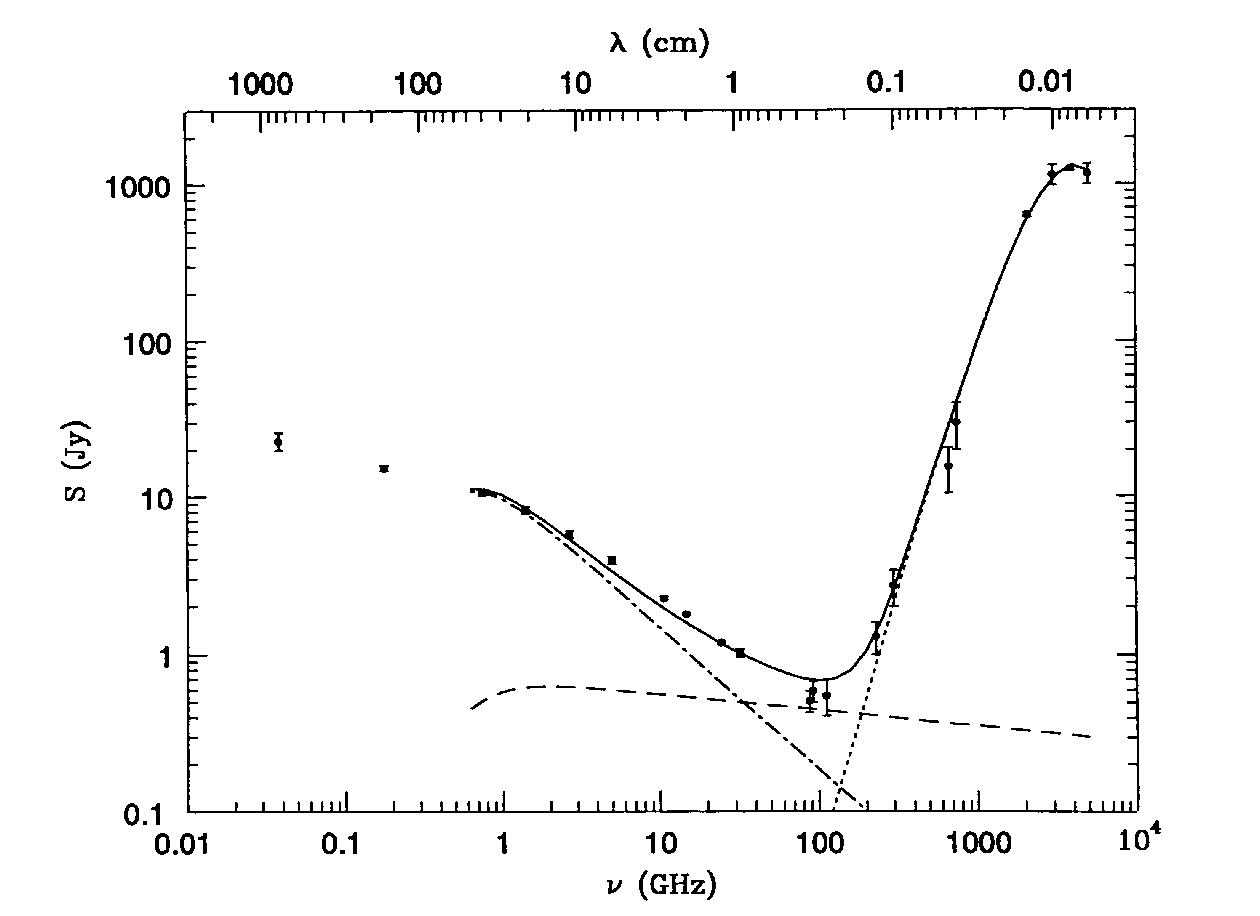
\includegraphics[width=\textwidth]{images/M82Spectrum.png}
\caption{\label{plot.m82.spectrum} Radio and far-infrared spectrum for galaxy M82, as estimated \href{https://www.cv.nrao.edu/course/astr534/FreeFreeEmission.html}{by the NRAO online course} (\url{https://www.cv.nrao.edu/course/astr534/FreeFreeEmission.html}). The flat curve corresponds to free-free emission, while synchrotron radiation (negative slope) and thermal dust emission (postive slope) dominate at low and high frequencies respectively.}
\end{figure*}


\subsection{Synchrotron Radiation}

\pg
Synchrotron radiation is the dominant mode of emission for extragalactic sources at low wavelengths. As such, it will be covered in greater detail than the other mechanisms above, which are important in other bands (and therefore relevant for multi-spectral analysis) but much less relevant to LOFAR observations. This section draws heavily from Garret Cotter's \href{http://www-astro.physics.ox.ac.uk/~garret/teaching/}{high-energy astrophysics lectures}\footnote{\url{http://www-astro.physics.ox.ac.uk/~garret/teaching/}}, as well as Alan Loh's \href{http://theses.md.univ-paris-diderot.fr/LOH_Alan_2_va_20160930.pdf}{doctoral thesis} \citepads{alan} and \href{https://www.cv.nrao.edu/course/astr534/SelfAbsorption.html}{the NRAO online course}\footnote{\url{https://www.cv.nrao.edu/course/astr534/SelfAbsorption.html}}.

\pg
Synchrotron radiation (or ``magnetobremsstrahlung") occurs when the trajectory of a relativistic charged particle is guided by a magnetic field. As the German name suggests, it is the magnetic equivalent of free-free radiation. It is the tracer of very energetic processes, such as the interaction between AGN jets and the intergalactic medium. In the low-energy regime, it is also known as cyclotron radiation, after the device in which it was first measured in a laboratory. %, and in non-relativistic regimes, it is known as gyro radiation. 

\pg
The synchrotron power spectrum of a population of electrons with exactly the same energy is a function of its Lorentz factor and its emission angle\footnote{The emission angle is the angle between the electron's total velocity (including z-axis) and its radial velocity.} \citepads{1994hea2.book.....L}. The typical radiation spectrum for a single electron is shown in \cref{fig.synchrotron.1electrion} as a function of the critical frequency, which is itself a function of the emission angle $\theta$, the Lorentz factor $\gamma$ and the magnetic field strength $B$: $\nu_c=3/2\frac{\gamma^2 e B}{2\pi m_e c}\sin(\theta)$. $e$ and $m_e$ are the electron charge and mass, respectively.
%$\nu_c=3/2\frac{\gamma^2 e B}{2\pi m_e c}\sin(\theta)$.
\begin{figure}[!h]
\centering
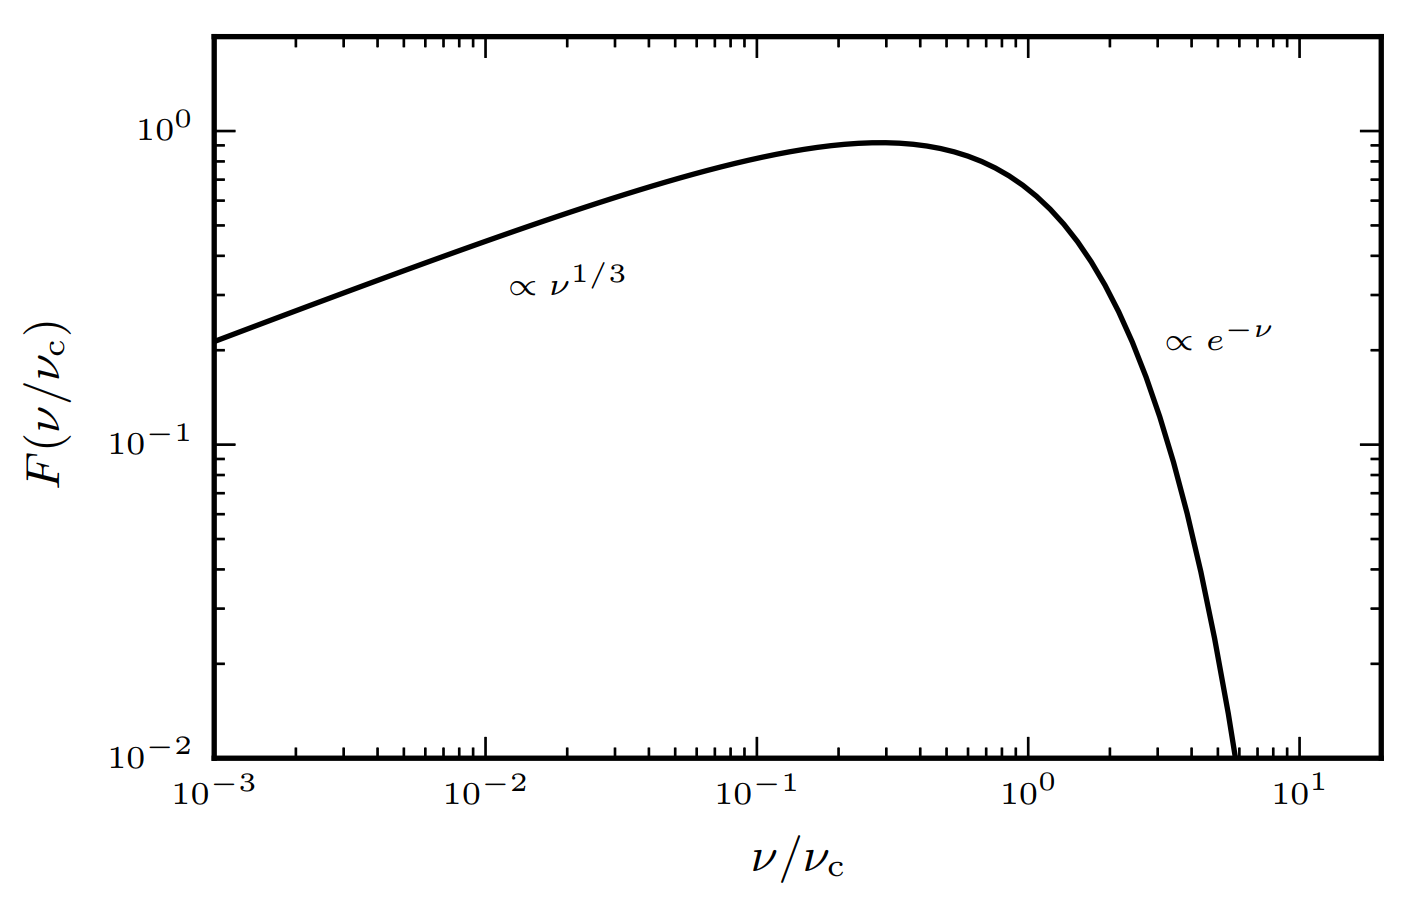
\includegraphics[width=0.9\textwidth]{images/Synchrotron-single-electron.png}
\caption{\label{fig.synchrotron.1electrion} Characteristic spectrum of synchrotron emission for a population of single-energy electrons. Arbitrary unit scale. Source: NRAO online course: \url{https://www.cv.nrao.edu/~sransom/web/Ch5.html}}
\end{figure}

\pg
Of course, in reality, we know that electron populations in astrophysical sources do not all share exactly the same energy when emitting. The effect of the electron energy distribution must therefore be taken into account. Because the population in question is energised through non-thermal processes, its energy distribution is not Maxwellian, and is generally written as a power law: $S(E) \propto E^\alpha \rightarrow S_\nu \propto \nu^{-\alpha}$, where $\alpha$ is the object's spectral index. Note that the index of the energy distribution (which relates the number of electrons at a given energy) is different from the synchrotron index, with the two related by the following equation: $\alpha=-(\gamma-1)/2$.
The question now becomes: what $\alpha$ is appropriate for what kind of object? Does every source have the same $\alpha$ at all frequencies? Do all synchrotron sources have the same spectral index at a given frequency, and if not, what does this tell us?

\pg
To answer these questions, we must recall that so far, we have assumed that every photon emitted through synchrotron radiation reaches us. This is not necessarily the case in practice: it is possible for a given photon to be scattered (i.e. absorbed \& re-emitted) by surrounding high-energy electrons. The likelihood of this occurring at a given frequency is a function of the absorption cross-section, and is a complex quantity to calculate (see \citetads{1994hea2.book.....L}  pp258-260). Suffice to say that at longer wavelengths (lower frequencies) absorption is more effective, and at shorter wavelengths (higher frequencies) the underlying electron energy power-law  distribution begins to dominate. An example is shown in \cref{fig.synchrotron}, taken from \citetads{2007A&A...471.1105T}.

\begin{figure}[!h]
\centering
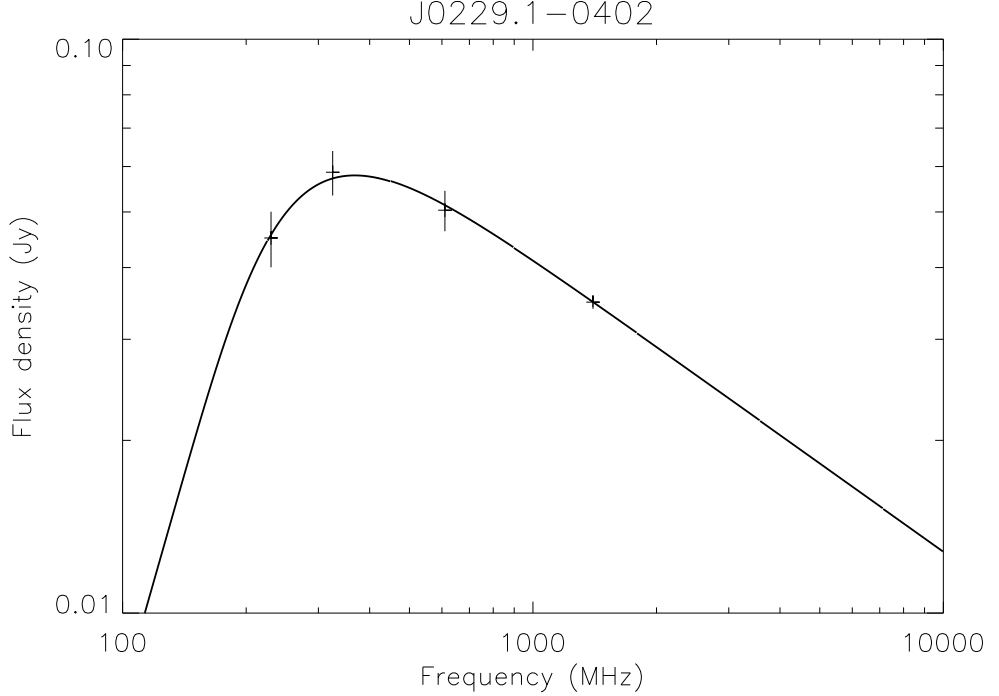
\includegraphics[width=0.8\textwidth]{images/synchrotron-spectrum.png}
\caption{\label{fig.synchrotron} Power spectrum for J0229.1-0402. Source: \citetads{2007A&A...471.1105T}.}
\end{figure}

\pg
In the optically-thick regime, we know that the most efficient radiation mechanism is simple black-body radiation, and so the power spectrum at a given frequency can be defined in terms of an ``electron temperature". In the Rayleigh-Jeans approxmation (valid as we are explicitly in the low-frequency regime), this gives $S_\nu \propto \nu^{5/2}$, or $\alpha=5/2$. 
In the optically-thin regime, meanwhile, we recover a mixture of the underlying power-law distribution ($S_\nu \propto \nu^{-\alpha}$) and black-body radiation (which has a frequency-dependent $\alpha$). Empirically, we generally observe $\alpha \sim 0.7$.


\subsection{Free-Free Radiation}
\pg
Free-free or ``bremsstrahlung" (``braking") radiation occurs when the trajectory of a charged particle is deflected by an electric field. This non-thermal emission mechanism is the dominant mechanism in HII regions (which contain ionised hydrogen), where star formation has previously taken place. It is called free-free emission because it is produced by free electrons deviating off ionised hydrogen (i.e. protons) without being captured. When the underlying electron distribution is Maxwellian, it is referred to as thermal Bremsstrahlung.

\pg
This emission's spectrum is heavily dependent on a number of factors: including frequency, temperature, and critically, free-free opacity $\tau_\nu$, itself a function of electron density. It is characterised by a knee in its spectrum, occurring where $\tau_\nu\sim 1$. This knee delineates two regions with different spectral indices; $\alpha \sim -0.1$ at higher frequencies, and $\alpha \leq 2$ at lower frequencies. This gives a characteristic shape, shown in Fig. \ref{plot.freefree.spectrum}.
\begin{figure*}[!h]
\centering
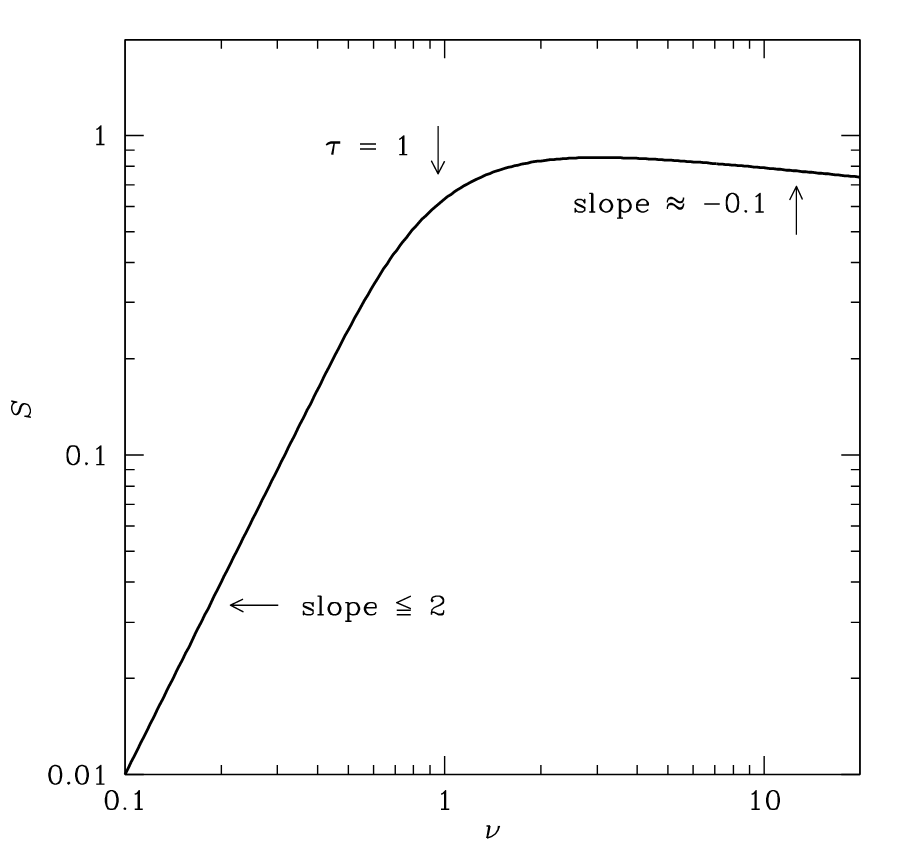
\includegraphics[width=0.7\textwidth]{images/freefree.png}
\caption{\label{plot.freefree.spectrum} Characteristic spectrum of free-free radiation. Arbitrary unit scale. Source: NRAO online course: \url{https://www.cv.nrao.edu/course/astr534/FreeFreeEmission.html}.}
\end{figure*}

\pg
As we can see, this spectrum falls off sharply with decreasing frequency. As such, while it is expected to dominate over thermal emission in the absence of synchrotron radiation, it is synchrotron emission that is expected to dominate overall - if present - at the low frequencies of our observations, which are done with LOFAR. Free-free emission acts as a tracer for star formation and other "gentler" physical processes detected at low radio frequencies.



\clearpage
\section{LOFAR: The LOw-Frequency Array}

\pg
Our observations have all been made with the LOw Frequency Array LOFAR \citepads{2013A&A...556A...2V}. In this section, we describe its technical properties and its current state of the art. In particular, the distinction between ``Dutch" LOFAR and ``international" LOFAR - and the technical problems associated with each - will be made explicit in this section.

\pg
LOFAR is a SKA pathfinder instrument, which means that it serves not only as a cutting-edge instrument in its own right, but does so with the explicit aim of serving as testing grounds for technologies \& techniques which could be usefully implemented in the SKA. It is in this context, for example, that trailblazers such as NenuFAR \citepads{2012sf2a.conf..687Z}, a low-frequency extension of LOFAR, are tested. LOFAR is an interferometric array, with each of its elements made up of antennas combined into a phased array, themselves forming an interferometer. It thus consists of antennas which are combined to form stations, which are themselves distributed throughout the Netherlands and Europe.
\begin{figure}[h!] 
  \begin{minipage}[c]{0.45\linewidth}
    \centering
    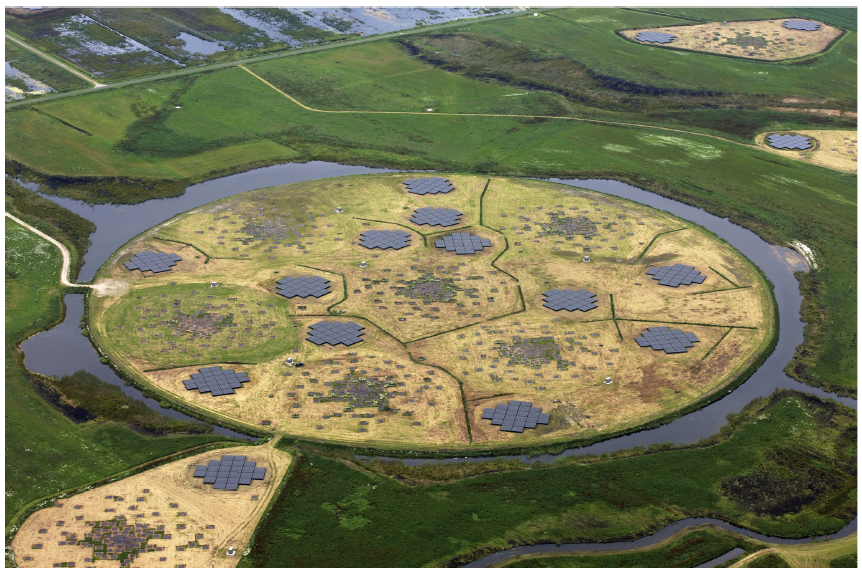
\includegraphics[width=\linewidth]{images/superterp.png}
	\subcaption{\label{fig.lofar.superterp} LOFAR core, known as the Superterp.}
%    \vspace{4ex}
  \end{minipage}
  \hfill
  \begin{minipage}[c]{0.45\linewidth}
    \centering
    \includegraphics[width=.5\linewidth]{images/{lofar-core-map_grey.jpg}}
    \subcaption{\label{fig.lofar.core} Distribution of the so-called LOFAR "core" stations, which include the Superterp.}
%    \vspace{4ex}
  \end{minipage} 
  \begin{minipage}[c]{0.45\linewidth}
    \centering
    \includegraphics[width=\linewidth]{images/{Distribution_Remote_Stations}} 
    \subcaption{\label{fig.lofar.remote} LOFAR with both "core" and "remote" stations.}
%    \vspace{4ex}
  \end{minipage}
  \begin{minipage}[c]{0.45\linewidth}
    \centering
    \includegraphics[width=.9\linewidth]{images/{Distribution_International_Stations}} 
    \subcaption{\label{fig.lofar.international} International LOFAR. Newer stations (one in Ireland, three in Poland) are not shown here.}
%    \vspace{4ex}
  \end{minipage} 
\caption{\label{fig.lofar.distribution} Geographic location and distribution of LOFAR stations, explicitly showing what is meant by Superterp, core, remote and international stations. All images from \href{https://www.astron.nl/radio-observatory/astronomers/users/technical-information/lofar-array-configuration/lofar-array-conf}{the official ASTRON website}: \url{https://www.astron.nl/radio-observatory/astronomers/users/technical-information/lofar-array-configuration/lofar-array-conf}}
\end{figure}


\pg
There are two bands to LOFAR, which are known as LOFAR-HBA (High-Band Antennas) and LOFAR LBA (Low-Band Antennas). \cref{fig.lofar.superterp,fig.fr606.layout} show the layout of the 6 innermost core stations and the French international LOFAR station, respectively.
\begin{figure}[h!]
\includegraphics[width=0.5\textwidth]{images/{LOFAR_NenuFAR.jpg}}
\caption{\label{fig.fr606.layout} Layout of FR606, the French LOFAR station at Nancay. At bottom left are the HBA tiles, bottom right the LBA dipoles, and at the top are some of the NenuFAR tiles.}
\end{figure}



\pg
We see the presence, in both cases, of two very different antenna types. One of these antenna types is not a single antenna, but rather a phased array: 16 antenna dipoles distributed in a $4 \times 4$ array. International LOFAR stations include 96 such tiles, distributed in a ``filled-disk" pattern, where the disk fill ratio is determined by the size of the tile. Dutch ``remote" stations have 48 such tiles spread into 2 disks (HBA\textunderscore INNER and HBA\textunderscore OUTER), while ``core" station HBA tiles are split into two 24-tile crosses. This pattern is shown in \cref{fig.hba.tile}. The antennas from each tile are combined into a phased array with a single ``tile beam", and all tile beams are themselves combined as a phased array into a station beam\footnote{Reference: \href{https://www.astron.nl/radio-observatory/astronomers/technical-information/antennae/antennae-description}{ASTRON technical description}: \url{https://www.astron.nl/radio-observatory/astronomers/technical-information/antennae/antennae-description}}.% This station beam is then pointed digitally.
\begin{figure}[h!]
\includegraphics[width=0.45\textwidth]{images/{Schematic-diagram-of-a-24-tile-LOFAR-HBA-station-A-tile-is-made-of-16-dual-polarization.png}}
\caption{\label{fig.hba.tile} Layout of a single HBA tile. Source: \href{https://www.researchgate.net/profile/Sarod_Yatawatta/publication/281316394/figure/fig1/AS:614002589720576@1523401033149/Schematic-diagram-of-a-24-tile-LOFAR-HBA-station-A-tile-is-made-of-16-dual-polarization.png}{Sarod Yatawatta researchgate profile}}
\end{figure}



\pg
LBA antennas, use a very simple - and cost-effective - design. A typical LBA antenna is shown in \cref{fig.lba.ant}. 96 such antennas are spread in a semi-random pattern in each LOFAR station\footnote{Reference: \href{http://www.lofar.org/about-lofar/system/lofar-numbers/lofar-numbers}{LOFAR.org website}: \url{http://www.lofar.org/about-lofar/system/lofar-numbers/lofar-numbers}}. In Dutch stations, 48 of these are used at all times. They are combined as a single phased array.
\begin{figure}[h!]
\includegraphics[width=0.45\textwidth]{images/{lba.png}}
\caption{\label{fig.lba.ant} Picture of a single LBA antenna. Source: \href{https://i2.wp.com/lofar.ie/wp-content/uploads/2017/04/lba.png?resize=1500\%2C1000}{LOFAR technology website.}}
\end{figure}
\pg
LOFAR-HBA is sensitive to higher frequencies, from 120 MHz to 240 MHz\footnote{Reference: \href{http://www.lofar.org/about-lofar/system/lofar-numbers/lofar-numbers}{LOFAR.org website}: \url{http://www.lofar.org/about-lofar/system/lofar-numbers/lofar-numbers}}. It has a smaller field of view than LOFAR-LBA, but a better angular resolution. 
\pg
The dipole design frees observers from the need to physically point antennas at all: the final station pointing is achieved by digitally introducing delays in the recorded phase before averaging the data. In this sense, the pointing is achieved in a similar way as individual HBA tile pointing, albeit . The LBA antennas are receptive to signals emitted in the 30-80 MHz frequency range.

\pg
At the time of writing, use of the LBA data is still relatively new, as its calibration is a very tricky problem. For similar reasons, international LOFAR (i.e. the full LOFAR array) has not been used, at the time of writing, to create wide-field survey images. A large part of the work described in this manuscript consists of reaching a point where full use can be made of international LOFAR, in a streamlined and repeatable way. 



\clearpage
\section{This Thesis}

\pg
The work done in this thesis can be summarised as the development of a new algorithm for mitigating calibration artefacts in radio-interferometric images, and its application to a peculiar famous extragalactic field. Because our data volumes put radio interferometry in the domain of ``Big Data" (there are $\sim$245TB of LOFAR data centred on the Extended Groth Strip, for example), there is a very real need for fast, reliable methods with which to improve interferometric images. This algorithm follows from an improved understanding of the noise properties of interferometric images, and can be understood as a way to better constrain the flux distribution in images by minimising the presence of artefacts. This, in turn, helps self-calibration convergence by improving the image resulting from each imaging step of the self-calibration process. 

\pg
We then outline the application of this work, along with other modern tools, to the creation of a large, deep and high-resolution image of a rich patch of sky. While this approach is potentially extremely rewarding in terms of the science one can do with its resulting maps, it is also uniquely complicated. There exist many LOFAR HBA ($\sim$120-240 MHz) sky surveys \citepads[cf.]{2016MNRAS.460.2385W,2017A&A...598A.104S}, but they do not yet make use of international LOFAR, and are thus limited in resolution ($\sim 5''$). And while there are surveys made at LOFAR frequencies ($\sim$150MHz) with other instruments \citepads[e.g.]{2017A&A...598A..78I}, they do not match the resolution attainable with international LOFAR. The aim of our image is then to show that the international LOFAR stations can be used to create a radio image that matches HST/ACS resolution - which would allow for significant cross-matching and source analysis, since there is HST data available for the field being imaged, the Extended Groth Strip (EGS). This would not be a true survey, but more of a proof of concept: the application of new tools and the development of an appropriate strategy to image a large patch of the sky with the full LOFAR array. This image would have better resolution than FIRST \citepads[see][and references therein]{2015ApJ...801...26H}, which has a $4''$ resolution, relatively low sensitivity, and no short baselines (thereby missing diffuse emission and extended structure) at $\sim$1.4 GHz, while still being sensitive to diffuse emission due to the use of the LOFAR core stations. 
%Finally, there will of course be the SKA1-MID survey once the SKA is operational; this survey is expected to provide excellent resolution, sensitivity, and good $uv$-coverage, making it sensitive to diffuse emission as well as point sources.

\pg
Making this image is possible only because LOFAR observations of the Extended Groth Strip includes an extremely bright source, 3C295, in their field of view. This is both a blessing and a curse: unless this source is properly modeled and subtracted, it will pollute images of the EGS. However, because it is so bright, it can serve as a good calibrator source for the LOFAR international stations - if a good enough model of 3C295 can be made and used to calibrate these stations, then high-resolution images of the EGS becomes attainable. This would give access to a large population of radio AGNs at high resolution, observed at a large range of frequencies, and many of which lie at redshifts near the peak of star formation; this improvement of our low-frequency understanding of these objects could, in turn, lead to an improved understanding of these objects more generally.

\pg
To really be able to perform wide-field images using the full LOFAR array, we cannot rely on the happy circumstances we find ourselves in for our applications project: a much more thorough and reliable approach is necessary. The work of the LOFAR long-baseline team \citepads[e.g.]{2016A&A...595A..86J} shows that kind of approach: in our project, we test specific strategies and approaches which are complimentary to their work, but cannot be applied more generally without their results.

%\pg
%In this context, a sky survey made using international LOFAR would be competitive until the SKA-MID survey (and considering it maps the Northern sky rather than the Southern sky, would arguably remain competitive even then). It would also allow LOFAR to fulfill the role of pathfinder in a very literal way, by providing datasets on which algorithms and imaging strategies could be tested before handling SKA data volumes in real-time.
%
%\pg
%Making a high-resolution full-sky survey using international LOFAR is thus arguably useful in and of itself in terms of interferometric techniques \& instrumentation. What then of its science value? The two most obvious advantages of a good large-sky survey are that they are complete (i.e. they are an accurate sample of the underlying source distribution, up to the survey's limiting flux)  while still giving information on rare outlier objects which may happen to lie in the field. This gives us access to a wealth of statistics from which to derive more robust estimations of population distributions. %Furthermore, depending on the quality of a given survey, it might even be able to provide such statistics simultaneously for various different fields of scientific interest.
%
%\pg
%Of course, LOFAR is already providing such catalogues - LOTSS \citepads[see][and references therein]{2017A&A...598A.104S}  is only the first of many to come. But these catalogues do not make use of the LOFAR international stations, and thus do not make full use of LOFAR's resolution ($5''$ resolution vs. $0.5''$).  This is so due to the technical challenges introduced by the use of international stations, which are due to decorrelation and an already limited signal-to-noise on those very short spatial frequencies.
%
%\pg
%What would they add to a LOFAR catalogue? A high-resolution sky survey has all the advantages listed above with more besides. For AGN science, for example, the higher resolution gives information on smaller scales, which is very relevant to study the turbulent processes in the lobes and the nearby intergalactic medium. This can give better insight into AGN feedback, for example \citepads[e.g.]{2007NewAR..51..168B,2016A&A...593A.118Q}. We also know that there exist small AGNs: size therefore matters, and resolving these small AGNs (which tend to lie at larger redshifts, hence their smaller angular size) can give extremely salient information on AGN population distributions as a function of the age of the universe. Indeed, for AGN science, the LOFAR international baselines can be the difference between having absolutely no information on size distribution (no resolved AGN) and knowing everything about the AGN size distribution within a given extragalactic field. Finally, resolving sources is very relevant to spectral studies of AGN populations: we know very little about the physics of AGNs at low frequencies. Information on large populations of resolved sources (allowing us to separate compact structure from extended emission) is a prerequisite to begin the statistical work needed to understand these low-frequency AGN physics. As such, the international baselines can bridge a critical gap in the data available to peers studying AGN science.
%
%\pg
%AGN science is far from the only field which could benefit from the sub-arcsecond resolution that international LOFAR could provide. High-resolution imaging can be of tremendous interest to the study of star-forming galaxies: it could give insight into cosmic ray structure and access to spectral information. This is relevant because the entire star-forming history of galaxies is encoded in radio emission, but can only be accessed with sufficient spectral information and spatial resolution. A high-resolution survey, in particular, allows comparisons between optical and radio emission for known star-forming galaxies on a truly industrial scale, which would allow for the mapping of free-free absorption, supernova remnants, HII regions, etc...onto optical maps, and this for sources going up to high redshifts.
%
%\pg
%Of course, this does not run the full range of science cases which would benefit from high-resolution maps of large parts of the radio sky. Colleagues studying gravitational lensing would benefit greatly from large samples of lensed galaxies. Resolved extragalactic recombination lines (for bright objects) would doubtlessly interest peers studying galactic evolution. We expect these samples to be a natural byproduct of a large, high-resolution map of the radio sky: if they do not appear, that could indeed be a very interesting scientific result in and of itself.
%
%\pg
%More generally, high-resolution surveys provide high-resolution images of everyone's favourite objects and sources. It allows for better optical matching and identification, which is particularly relevant e.g. when needing to associate either a low-z or high-z sources to optical counterpart sources (in the case of the Extended Groth Strip, for example, using the international stations means matching the Hubble Space Telescope's resolution). They are thus a strong contribution to multi-wavelength datasets. It also improves the image's sensitivity to compact sources embedded in diffuse emission: if the source is better-resolved, then the emission associated with compact sources is more easily separated from emission emitted by its surroundings. This can be of tremendous help in image interpretation. Finally, actually resolving objects allows us to have better morphological classification for compact objects, which can be extremely useful e.g. when interested in AGN populations vs star-forming galaxy populations.

\subsection{Algorithmic Developments}

\pg
A significant portion of the work done as part of this thesis was on investigating the relationship between calibration gain errors and calibration artefacts in the image-plane. What started as an attempt to properly write a weighting scheme to down-weigh poorly-calibrated visibilities\footnote{i.e. to justify weighting visibilities by a function inversely proportional to the variance of the associated residual visibilities.} eventually became a formal relationship between these quantities, showing both the behaviour of image-plane variance as a function of direction but also of pixel covariance over the full image. This work is shown in much greater detail in \cref{chapter.paper}.

\pg
The key finding of our algorithmic work is a fundamental relationship between the covariance matrices of residual visibilities and the covariance of pixels in the image-plane: the ``Cov-Cov relationship'' between visibility covariance and image-plane covariance. The pixel variance and covariance in the image-plane are determined by a ``noise-PSF'', convolved with every pixel in the sky. This also means that thermal noise in interferometric images is correlated between pixels, and that this correlation is given exactly by the PSF: in the limit of an empty, non-deconvolved sky, we therefore properly model the thermal noise properties of its interferometric images. This noise-PSF is the product of the Fourier transforms of the calibration gain covariance matrix with each cell mapped not from $uv$ space to $lm$ coordinates\footnote{$uv$ space is where interferometric measurement coordinates lie, and $lm$ coordinates are the cardinal sines on which the inverse Fourier transform of the visibilities are mapped.} but rather between their respective covariance spaces - from a new {differential Fourier plane (henceforth ``$\left(\deltu\deltv\right)$''-plane) to the image-plane covariance space $\deltl\deltm$. This image-plane covariance space describes} the variance in each pixel and the covariance between pixels\footnote{{The noise-PSF also relates $\delta w$ to $\delta n$, as shown in our matrix formalism, but we do not explicitly reference this in the text for the sake of brevity, as visibility space is usually referred to as ``the UV-plane'' in literature, rather than ``the UVW-space''. For more information, see \cref{chapter.paper}}}. It describes the expected calibration artefacts and noise level around each source, does not vary as a function of direction, and is convolved with each source in the field to yield the final error map. Because all unwanted (in our case, unphysical) signal can be thought of as noise, we will refer to {the pixel variance map} as the ``noise-map''.

\pg
Based on this theoretical finding, we develop a weighting scheme algorithm with which to improve the noise properties of interferometric images by down-weighting either visibilities with high variance in their calibration residuals, or visibilities which are strongly correlated to others in their calibration residuals. We implement a robust version of the first weighting scheme, which relies on an antenna-based estimate of the visibility variance. 


\subsection{Imaging the Full Primary Beam}


\pg
In this section, we briefly describe previous observations of the Extended Groth Strip (EGS), an extragalactic field with a rich multi-wavelength coverage described in Table \ref{table.EGS.observation}. It has been long observed as part of the All-Wavelength Extended Groth Strip International Survey collaboration (AEGIS, \citetads{2007ApJ...660L...1D}), which later became part of the CANDELS collaboration (\citetads{2011ApJS..197...35G}). The field is centred at $\alpha=14^h17^m,\delta=+52^o 30'$, placing it between the tail of Ursa Major and Draco. Its size is $0.7'\times 0.1'$. It has notably been the subject of very deep Hubble Space Telescope observations, which the international LOFAR could attempt to match. 

\begin{table}[h!]
\begin{tabular}{cccc}
Telescope    & Band    & Resolution  & Area \\\hline
Chandra      & X-ray   & $0.5''-6.0''$ & $17'\times 120'$ \\
GALEX        & UV      & $5.5''      $ & 1.25$^\text{o}$ diameter \\
HST/ACS      & Optical & $0.1''      $ & $10' \times 67'$\\
HST/NICMOS   & Optical & $0.35''     $ & 0.0128 deg$^2$\\
Megacam      & Optical & $1.0''      $ & 1 deg$^2$\\
IRAC         & IR      & $2.0''      $ & $10' \times 120'$ \\
Spitzer      & IR      & $5.9''-19'' $ & $10'\times 90'$\\
VLA          & Radio   & $1.2''-4.2''$ & $30' \times 80'$
\end{tabular}
\caption{\label{table.EGS.observation}Table recapitulating the multi-wavelength coverage of the Extended Groth Strip, with observations performed as part of the AEGIS (later, CANDELS) collaborations.}
\end{table}


\pg
Our data consist of an observation centred on the EGS. The LOFAR beam (i.e. how much of the sky LOFAR is sensitive to at a given time) is much larger than the EGS. As such, our measured visibilities includes contributions not just of sources in the EGS, but also from those all around it - including a very bright 3C\footnote{Third Cambridge Catalogue of Radio Sources, a 1959 survey of of the Northern radio sky}  source, which will be discussed at length below. Due to technical limitations (i.e. available memory), it is not feasible to image the full LOFAR primary beam at once at international LOFAR's  $0.1''$ resolution. As such, we begin by imaging at a lower resolution, and thus do not use the international stations at first. This allows us to create a low-resolution model of all the sources in the primary beam before proceeding to international station calibration, giving us a sanity check for core and remote station gains. It also allows us to subtract out-of-field sources when imaging the EGS at high resolution.

\pg
Initial direction-independent calibration is done using Prefactor, the same pipeline as for the Lofar Two-metre Sky Survey, followed by direction-dependent calibration with the killMS-DDF facet-based pipeline \citepads[LOTSS,][]{2017A&A...598A.104S}. %This killMS-DDF facet-based pipeline \citepads[cf]{2015MNRAS.449.2668S,2016ApJS..223....2V,2017arXiv171202078T} is then used to perform direction-dependent calibration for the entire LOFAR primary beam. This allows us to reach a noise threshold of $\sim$233$\mu$Jy.

\pg
This work, and its results, are shown in \cref{section.EGS.lowres}. Note that the AEGIS observations summarised in \cref{table.EGS.observation} do not cover the full LOFAR primary beam. The sources observed at low resolution are therefore matched with Sloan Digital Sky Survey (SDSS, \citetads{2000AJ....120.1579Y}) images. Overlays are shown to highlight the wealth of interesting sources, and their optical counterparts, which can be picked up as a byproduct of high-resolution maps of the radio sky. We select 12 particularly interesting sources and show the results of source matching for these candidates. Overlays of the same SDSS images with NVSS (NRAO VLA Sky Survey, \citetads{1998AJ....115.1693C}) postage stamps are also shown for comparison. Many of the chosen sources do not lie within the Extended Groth Strip, and are therefore only imaged at low resolution, but high-resolution follow-up images and observations could be made should the need arise.


\subsection{3C295 and the Extended Groth Strip}


\pg
The brightest source in the primary beam of our observation is 3C295. It is one of the brighter sources in the Northern radio sky. It lies less than a degree away from the centre of the Extended Groth Strip, which has two important consequences: first, that it can potentially be used as a calibrator source for LOFAR; second, that unless well-modeled and subtracted at the observing instrument's maximum resolution, its sidelobes will pollute the EGS such that very little scientifically useful information might be recovered from a given observation. If we wish to image the EGS with international LOFAR, we therefore cannot rely on a low-resolution model: small errors in the exact location of 3C295's flux could corrupt most of the very long-baseline visibilities, thus making them useless. A high-resolution model of 3C295 is necessary for us to proceed.

\pg
The first step towards acquiring a deep, high-resolution image of the Extended Groth Strip is therefore to create a good, high-resolution model of 3C295 at LOFAR frequencies and for long baselines. Creating this model is one of the key results of this thesis. Starting from a high-resolution VLA model of 3C295, subbands selected across the LOFAR bandwidth are self-calibrated in iteratively greater numbers until a given noise threshold is reached. The flux scale is then boot-strapped based on the results of \citet{arse}. This ensures that 3C295 will be adequately subtracted from all corrected visibilities - including international baselines - and thus that images made using these visibilities will not be polluted by sidelobes from 3C295. 
The work done towards this goal is shown in \cref{section.3c295}. %, and its result - a high-resolution spectral model of 3C295 - is shown below.
%
%\pg
%\textcolor{red}{show key result here}

\pg
Before launching the EGS imaging run using all calibrated datasets, we measure the impact of direction-dependent effects on known sources in the field. Two direction-dependent effects are expected to dominate: decorrelation and differential gains. The first is modeled by the algorithms used in this thesis, whereas the second is a function of the gain variability as a function of distance from the calibrator. Eight calibrator sources, lying at various distances and directions from the calibrator source, are examined. They are summarised in \cref{table.LOBOS.sources}, which is reproduced below: note that number 6 is actually 3C295. Their distribution in the sky is shown in \cref{lbcs-coverage-image11}.

\begin{table}[h!]
\begin{tabular}{ccccc}
\# & RA [hms]    & Dec [dms]   & Dist. from EGS [deg.] & Dist. from 3C295 [deg.] \\\hline
1  & 14:30:18.72 & 52:17:29.80 & 2.041                         & 2.904 \\
2  & 14:19:44.44 & 54:23:04.58 & 1.928                         & 2.517 \\ 
3  & 14:21:20.05 & 53:03:46.00 & 0.864                         & 1.743 \\
4  & 14:21:09.41 & 51:22:32.46 & 1.294                         & 1.728 \\
5  & 14:11:50.32 & 52:49:02.66 & 0.844                         & 0.619 \\
6  & 14:11:20.23 & 52:12:04.30 & 0.915                         & 0.000 \\
7  & 14:08:07.00 & 52:55:11.36 & 1.409                         & 0.869 \\
8  & 14:08:09.76 & 52:44:46.56 & 1.354                         & 0.680 \\
\end{tabular}
\caption{\label{table.LOBOS.sources11}Table recapitulating the positions of all 8 chosen calibrator sources, along with their distance from the observation phase centre (EGS phase centre) and calibrator phase centre (3C295), respectively. Number 6 is 3C295.}
\end{table}
\begin{figure}[h!]
\includegraphics[width=\linewidth]{images/{image_full_ampphase_di_m.NS_Smooth.noise01.fitslbcs.egs.positions}.png}
\caption{Position of the calibrator sources around the EGS, overlaid on the widefield EGS image. LBCS6 is 3C295.}
\label{lbcs-coverage-image11}
\end{figure}
%\begin{figure}[h!]
%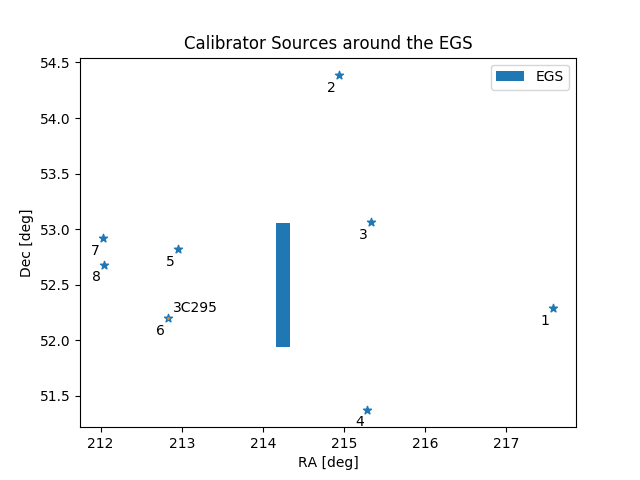
\includegraphics[width=0.8\linewidth]{images/EGS_LOBOS_scatterplot}
%\caption{Position of the calibrator sources around the EGS. Note that this is not projected properly onto the celestial sphere.}
%\label{bootes-coverage-image}
%\end{figure}

\pg
If directional gains are measured to have little or no impact, then direction-dependent calibration of the international stations will not be required. This is the ideal scenario, as it does not require the use of fringe fitting \citepads{1984ARA&A..22...97P}. If they are measured to have a significant impact, then direction-dependent calibration will be required for international LOFAR. We expect the angular scale of differential gain evolution to be of the order of a degree, and so most of the EGS should be relatively unaffected.
%
%\pg
%Having quantified the impact of directional gain errors on our field, we then proceed to a patchwise imaging of the EGS.

%
%
%\subsection{Imaging the EGS with LOFAR international stations}
%
%\pg
%if decorrelation is merciful, proceed to patchwise imaging of EGS by using the results from the sections above (DI calibration using 3c295 model, followed by subtraction of all sources seen at low-res except within the patch we want to image; image, change patch; repeat until all EGS imaged)
%
%\newpage


% % % Chapter 2 - intro
\cleardoublepage


\chapter{Techniques of Interferometry}
\minitoc

\pg
In this section, we contextualise the work done as part of this PhD by discussing the difficulties introduced by the combination of sparse $uv$-coverage and weak \emph{a priori} constraints on the sky brightness distribution. The conceptual framework which we rely on throughout this manuscript, the Radio Interferometer's Measurement Equation, is described in greater detail in  \cref{section.RIME}. We will begin by discussing radio interferometry itself. We will then discuss the so-called \emph{imaging problem}, and end by discussing the \emph{calibration problem}. Note that both of these are artifical subsets of the general inverse problem of radio interferometry. While in practice calibration is done before imaging, it is conceptually helpful to begin with imaging. Until we reach our introduction to radio interferometric calibration, we will therefore assume that calibration has been successfully carried out, and that we are working on the \emph{corrected visibilities}, i.e. gain-corrected visibilities. 

\pg
We start by linking interferometry to more concrete concepts: specifically, we will give a (very!) brief introduction to radio antennas and their characteristics. We will then use this introduction to show the advantages and drawbacks of radio interferometry, along with the concrete technical problems that the method introduces.

% will make the ideas and basis of radio interferometry more accessible by allowing us to explain the abstractions that interferometry relies on in terms of simpler instrumental configurations. We will then introduce the concrete problems that interferometry introduces: both a recapitulation of the venerable Zernike-van Cittert theorem \citep[cf.][]{1934Phy.....1..201V} and the problem of incomplete $uv$-cove	rage.



\clearpage
% !TeX spellcheck = en_UK


%
%\pg
%There exists a wide variety of methods used in imaging, from the venerable CLEAN algorithm\footnote{For an excellent beginner's introduction to CLEAN, the author heartily recommends \url{https://www.cv.nrao.edu/~abridle/deconvol/node7.html}} to cutting-edge compressed sensing and subspace deconvolution methods. We will begin this section by introducing a mathematical framework in which the problem of deconvolution can be understood, and proceed, from there, to discuss some of the deconvolution algorithms which can be used.
%
%\pg
%The formalism used in this section is based, in part or in whole, on that used by Cyril Tasse in [DDF paper].

\section{A Brief Introduction to Radio Astronomy}
\pg
Radio astronomy consists of observing the electromagnetic emission of astrophysical\footnote{And, famously, attempting to observe ``intelligent" sources \citepads[cf]{2017AAS...22911604E}} sources at very long wavelengths by means of radio antennas. These antennas measure a voltage proportional to variations in the electromagnetic field in all the directions they are sensitive to. Since astrophysical signals are weak, a good sensitivity is necessary. Achieving good sensitivity with radio antennas means having a very large collecting area - in this respect, they behave exactly the same way as optical telescopes. Similarly, when well-designed, they are diffraction-limited - this means that, once again like optical telescopes, their resolution is limited by their diameter.

\pg
However, because radio frequencies are so much lower, achieving a resolution comparable to e.g. the HST requires extremely large dishes. While there exist telescopes, both old and new, which work on this principle (from Arecibo Observatory, shown in \cref{fig.arecibo}, to the upcoming FAST telescope in China, shown in \cref{fig.FAST}), the associated technical difficulties (pointing is complex business, as are the associated optics requirements; maintenance costs are high, etc...) have made the single-dish approach prohibitive.

\begin{figure}[ht]
\centering
\begin{subfigure}{.48\textwidth}
\resizebox{\hsize}{!}{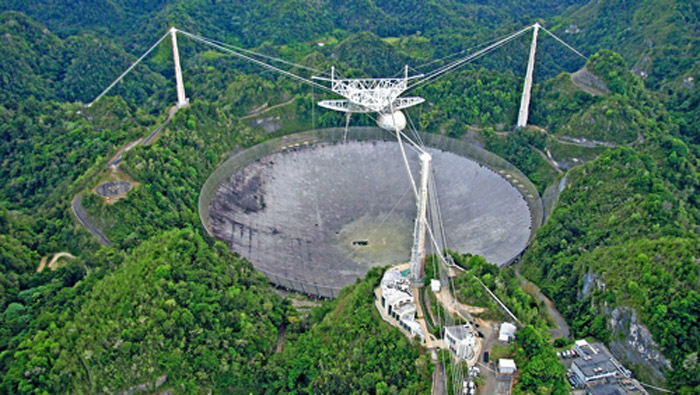
\includegraphics{images/20151101114231-0_8e7cc_c7a44aca_orig.jpg}}
\caption{\label{fig.arecibo} Arecibo telescope, in Puerto Rico.}
\end{subfigure}
\hfill
\begin{subfigure}{.48\textwidth}
\resizebox{\hsize}{!}{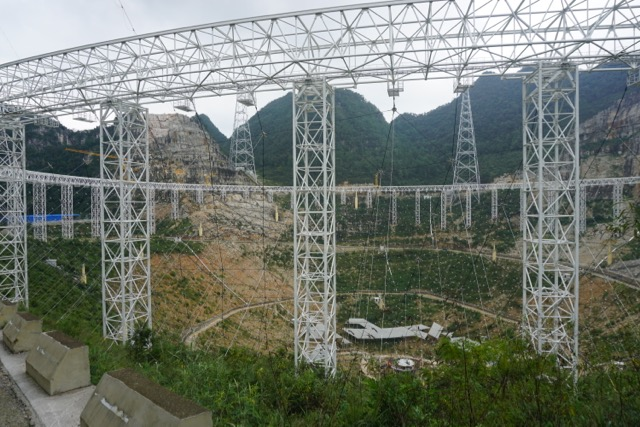
\includegraphics{images/FastTelescope_8sep2015.jpg}}
\caption{\label{fig.FAST} FAST telescope, in China}
\end{subfigure}
\caption{\label{fig.singleDishes} Examples of large single-dish radio telescopes.}
\end{figure}

\pg
One way to move past this technical limitation is to resort to interferometry: this is the topic of this section.





\section{Interferometry: Bypassing the Diffraction Limit}

\pg
There are two quantities of interest to all astronomers: sensitivity and angular resolution\footnote{Other kinds of resolution - in time and frequency, for example - are also extremely important to many astronomers, but are not what concern us here.}. An instrument's sensitivity is a function of its collecting area\footnote{It is also a function of technological factors, of course, but \emph{ceteris paribus}, a more sensitive telescope means a telescope with a wider collecting area}. Resolution, for well-designed instruments\footnote{By this, we mean that we assume that an instrument is also designed to optimise resolution.}, is limited by diffraction in the absence of atmospheric effects. This introduces specific issues in the radio domain. Radio waves have very long wavelengths - often comparable to meters, rather than the $\sim100-1000$nm wavelengths of optical light. Achieving a resolution comparable to those of optical telescopes would thus require making telescopes with apertures tens of millions of times larger than those already titanic instruments!

\pg
In practice, this technical constraint on resolution is one that astronomers are very interested in overcoming. This technical limitation therefore demands a technical solution. In practice, this solution consists of recourse to interferometric techniques. Indeed, interferometry can be thought of as the construction of a "sparse" dish, as illustrated in \cref{fig.aperture.synthesis}.

\begin{figure}[ht]
\centering
\begin{subfigure}{.43\textwidth}
\resizebox{\hsize}{!}{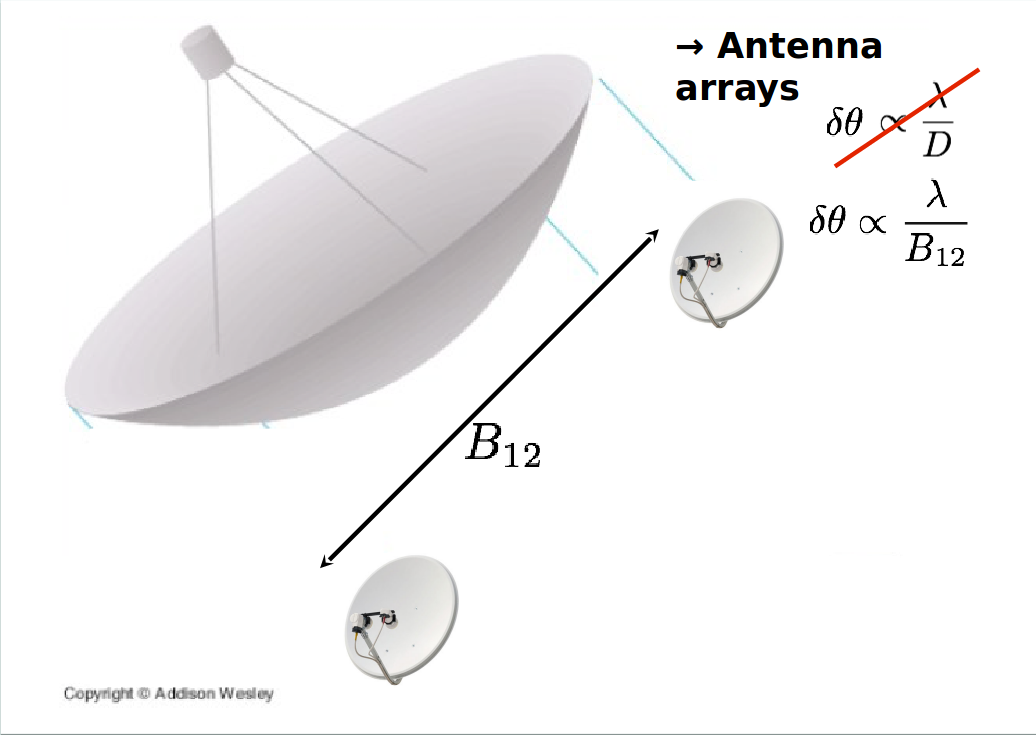
\includegraphics{images/baseline-resolution.png}}
\caption{\label{fig.baseline.image} A pair of dishes can surpass the resolution limit of its components.}
\end{subfigure}
\hfill
\begin{subfigure}{.43\textwidth}
\resizebox{\hsize}{!}{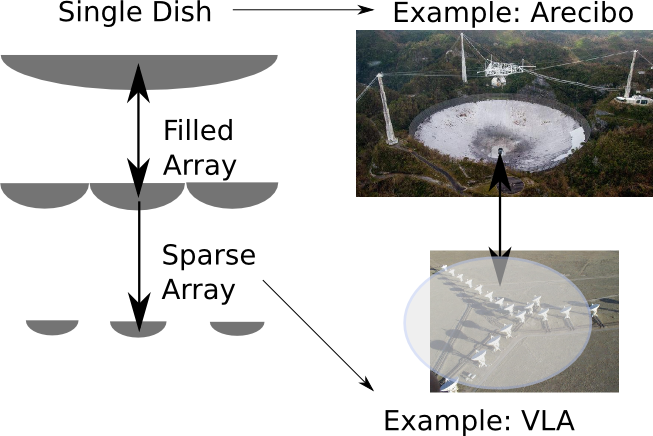
\includegraphics{images/sparseArray.png}}
\caption{\label{fig.arecibo.vla} With enough pairs of dishes, it is possible to synthesise a much larger dish.}
\end{subfigure}
\caption{\label{fig.aperture.synthesis} Illustration of the underlying principle of interferometry. The 27 dishes of the VLA can be thought of as "synthesising" a similar circular dish as Arecibo. This idea is the reason why radio interferometry is historically known as "aperture synthesis" in the literature of radio astronomy. \cref{fig.baseline.image} is copyrighted by Addison Wesley.} % \textcolor{red}{CHANGE FIG B. AS THE ELLIPSE IS NOT SEE-THROUGH}}
\end{figure}

\pg
Interferometric measurements are made as follows: the elements of the interferometric array (which can be single dishes or phased arrays\footnote{Described in \cref{sec.visibility}} of smaller antennas) measure a voltage. This voltage is correlated between antennas, as will be described shortly. Each of these correlations correspond to a single Fourier mode of the sky, as per the Zernike-van Cittert theorem (cf. \cref{sec.imag.psf}). They must be calibrated, by comparing the observations of a calibrator source and modelled visibilities. Calibration is described in much greater detail in \cref{section.RIME}. Then, the calibrated visibilities are used to reconstruct an image of the sky, which often requires deconvolution due to the sparsity of interferometric arrays.

\pg
The resolution improvement of interferometers does thus not come for free. To better understand the cost of interferometry, we will cover calibration after explaining the particularities of interferometers. We will begin with the properties of their core component: the baseline.

\subsection{The Baseline}

\pg
To define the baseline, we must begin by considering the geometric properties of an interferometric array. For now, let us assume that we are observing the sky above the array, a practice known as drift-scanning. A baseline then consists of the vector subtraction of the positions, in 3-dimensional space, of its two constituent antennas. Note that each antenna pair therefore has 2 corresponding baselines, since for each pair of antennas A and B we create baselines AB and BA. These distance vectors are then divided by the observing wavelength to give a dimensionless set of coordinates, known as $(u,v,w)$. These coordinates define the baseline entirely. 

\subsection{The Visibility}\label{sec.visibility}

\pg
We have defined what a baseline corresponds to: a vector coordinate in $(u,v,w)$-space. To each baseline we associate a measurement, which we call the \emph{visibility}. 
\begin{figure}[ht]
\centering
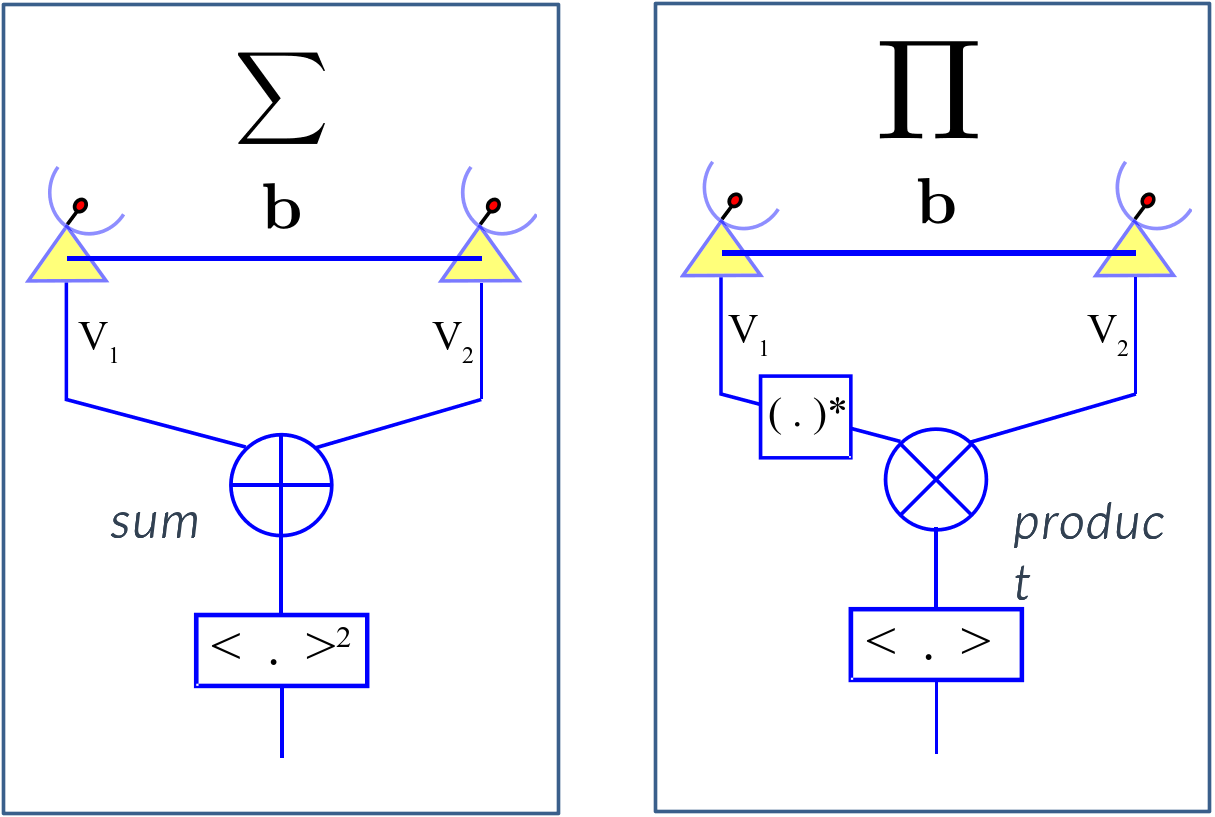
\includegraphics[width=.7\textwidth]{images/visibility-creation.png}
\caption{\label{fig.visibility} There are two ways to combine the voltages from two antennas into a visibility: they are sum-correlation and $\pi$-correlation. In this manuscript, we will only concern ourselves with the latter. Image credit: Julien Girard}
\end{figure}
The visibility associated with baseline $\mathbf{b}_{AB}$ is created by taking the voltage $V_A$ measured by antenna A, multiply it by the complex conjugate $V_B^*$ of the voltage measured by antenna B, average over the correlator dump time (i.e. the time over which the measurement is made). This scalar quantity is associated to the baseline position vector $\mathbf{b}_{AB}$. In other words:
\begin{align}
\mathbf{b}_{AB} &= \frac{\mathbf{x}_{B}-\mathbf{x}_{A}}{\lambda_\mathrm{obs}}\\
V_{AB}          &= \langle V_{A} V_{B}^*\rangle_{\delta t, \delta \nu} 
\end{align}
where $\langle \cdots \rangle_{i}$ denotes an averaging over quantity $i$. We see that a visibility is a complex vector quantity. We also see that $\mathbf{b}_{AB} = \mathbf{b}_{BA}^*$: the information of the visibility associated with baseline BA is contained in the visibility associated with baseline AB. This means that in practice, only half of the visibilities ever need be stored. What does the visibility measurement correspond to?
\begin{figure}[ht]
\centering
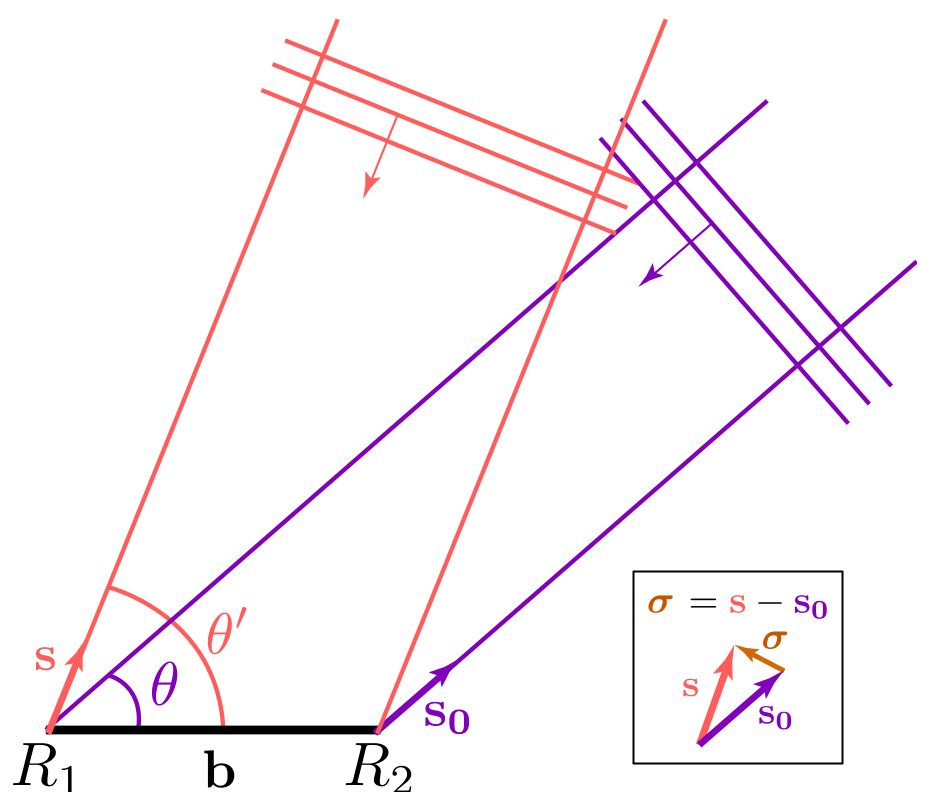
\includegraphics[width=.5\textwidth]{images/visibility-measure.png}
\caption{\label{fig.visibility.measure} Here, we assume that there are only two sources in the sky whose signal can be measured by our antennas. The final visibility is the sum of the visibilities associated with each individual source. Image credit: Julien Girard \citepads{julien}}
\end{figure}

\pg
The signals from different astrophysical do not interfere. They are measured additively in both antennas. Provided that the signal from each sources is coherent when observed by the dishes, the correlation between the voltages measured by antennas A and B will simply be the sum of the voltage correlations associated with individual sources. This is shown in \cref{fig.visibility}: the radio signal from two different sources, at two different locations, is picked up simultaneously by both radio antennas. Because only the correlation between both antennas is measured, the signals do not interfere: if the signal from each source gives a voltage $V_{p}^s$ for antenna $p$, then the additive property of electric fields means that the total visibility measured by baseline $pq$ can be written as:
\begin{align}
V_{pq}  &= \langle \left(\sum_{s} V_{p}^s\right) \left(\sum_{s} (V_{q}^s)\right)^*  \rangle_{\Delta t} \\
        &= \langle \sum_{s,s'} V_{p}^s (V_q^{s'})^*  \rangle_{\Delta t}\\
        &= \langle \sum_s V_{p}^s (V_q^{s})^* \rangle_{\Delta t} + \underbrace{\langle \sum_{s,s'\ne s} V_{p}^s (V_q^{s'})^* \rangle_{\Delta t}}_{=0} \label{eq.spatial.incor}
\end{align}
where the fact that signal from different sources is not coherent means that we average out cross-contributions (i.e. signal from $s\ne s'$). 
%\begin{align}
%V_{pq}&=\langle \left(\sum_{s} V_{p}^s\right) \left(\sum_{s} V_{q}^s \right)^* \rangle_{\Delta t} \right)\\
%      &=\langle\sum_{s,s'} \left( V_p^s\left(V_q^{s'}\right)^* \rangle_{\Delta t}
%\end{align}

\pg
Note that in Fig. \ref{fig.visibility.measure}, neither source is at the zenith. This introduces the notion of the \emph{effective baseline} which is shorter than the \emph{physical baseline} when measuring a signal from a source that is not at the zenith. Sources in different positions in the sky will be measured by an interferometric array, but the same array will have different effective baselines for different sources. To point an interferometric array in a specific direction in the sky, one must introduce a phase delay in each antenna (or, for fundamental interferometer elements such as the LOFAR tiles or NenuFAR, by playing with the cable length between each dish and the correlator). This is done by three means: delay tracking (which is exact only for the delay tracking centre\footnote{Source: \url{http://www.astron.nl/eris2013/Documents/2_laing_fundamentals_interferometry.pdf}, \url{https://science.nrao.edu/science/meetings/2016/15th-synthesis-imaging-workshop/SISS15Advanced.pdf}}, and corresponds to playing with the cable length between antennas in the interferometric array), antenna pointing\footnote{This maximises antenna sensitivity in a given direction, but is not done with LOFAR}, and fringe stopping\footnote{Fringe stopping consists of down-converting the signal received by antennas by mixing with a local oscillator. The geometric delay compensation is usually applied on this down-converted signal. Source: \url{http://www.gmrt.ncra.tifr.res.in/gmrt_hpage/Users/doc/WEBLF/LFRA/node74.html}}.
%Fringe stopping consists of measuring the beat between a predicted fringe rate (i.e. the period of the visibility sine wave corresponding to a point source out of phase centre; if the position of an array's antennas is well-known, this can be modeled accurately) and a known signal, e.g. the actual fringe rate (i.e. the fringe rate corresponding to the true period of the visibility sine wave). The difference between the two is a function of how well the antennas' positions are known. If they are well-known, then the phase information can still be measured, even without very fine sampling in time. } must be used to avoid taking a measurement every few milliseconds. 
This means that there are actually three different ``field centres", which are usually (but not always) set to be the same: the pointing (direction of maximum antenna sensitivity), the delay (which can be introduced in cable length) and the phase tracking (which consists of applying a known signal to the measured signal and recording the resulting heterodyne wave so as to keep a reasonable amount of post-correlation data without losing information on sources outside of the phase delay centre). The position of sources are then given in terms of the cardinal angle $\sigma$: this is the difference between the position of a source and the phase centre, which is where the array is pointing. For example, in \cref{fig.visibility.measure}, if we point antennas and introduce phase delays such that we are pointing the array towards Source 2, the position of Source 1 will be $\sigma$.


\subsection{The $uv$-plane}

\pg
%In general, interferometric design is such that the $w$ component of visibilities' $(u,v,w)$ coordinates is negligible (or can be put in a frame of reference where it can usually be approximated as such). 
For the sake of brevity, radio astronomers tend to talk of a $uv$-plane rather than $uvw$-space to describe visibility space. The set of $uvw$-values for all the baselines of an interferometric array is known as its $uv$-coverage, and defines the array's properties entirely.
For the VLA, for example, the instantaneous $uv$-coverage when observing the zenith will be as shown in Fig. \ref{fig.vla.uvcoverage}.

\begin{figure}[ht]
\centering
\resizebox{\hsize}{!}{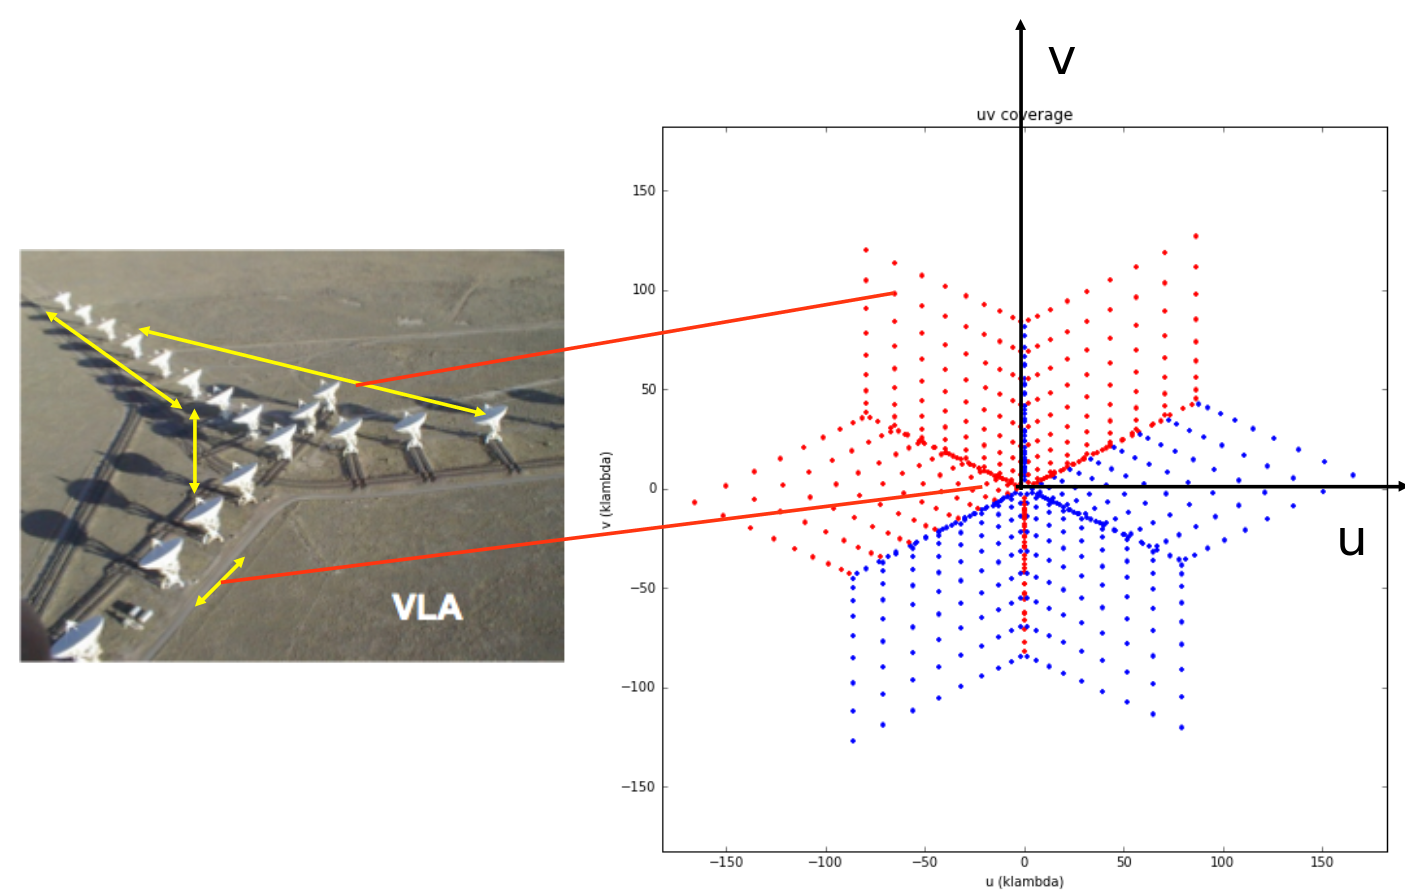
\includegraphics{images/vla-uvcoverage.png}}
\caption{\label{fig.vla.uvcoverage} The VLA contains 27 radio dishes placed as shown above. Each antenna pair between those 27 gives two single baselines, here, one red and one blue. Image credit: Julien Girard}
\end{figure}

%\pg
%The more points an array has in $uv$-space, the greater its $uv$-coverage and the better it will observe. This coverage can be improved for free in two main ways: firstly, the use of a technique known as supersynthesis (since the interferometer "synthesises" a dish at any given time, by assuming that the sky does not evolve over a certain time frame, we can treat different times as measurements of the same sky) and taking advantage of the frequency-dependence of $uv$-coordinates.The impact of both practices will be described in greater detail in \ref{sec.imag.psf}, but know that "$uv$-tracks" simply correspond to the $uv$-coverage of an interferometer observing over some period of time.

\pg
Individual antennas of an array can be pointed mechanically, and so the loss of antenna sensitivity in the direction of interest (and therefore the loss of net interferometric array sensitivity) can be minimised. But what happens to the array itself? It is useful here to go back to the illustration of Fig. \ref{fig.arecibo.vla}. Think of each dish in the array representing a "filled" segment of a massive but empty dish. By projecting our observation in a given direction, this dish goes from circular to elliptical.
\begin{figure}[ht]
\centering
\begin{subfigure}{.40\textwidth}
\resizebox{\hsize}{!}{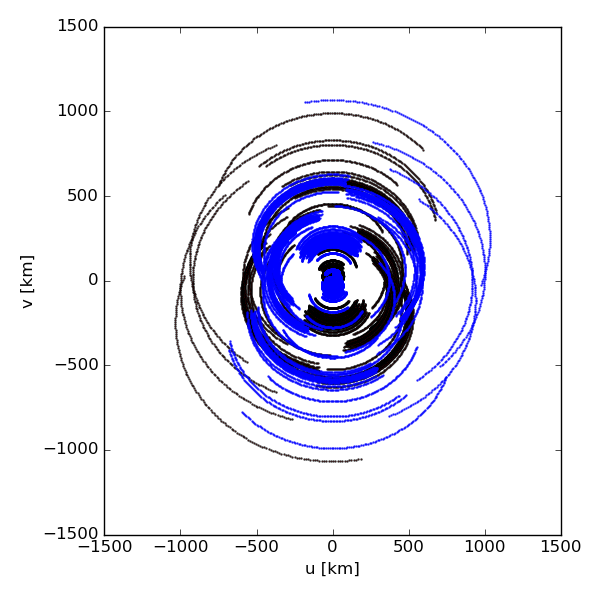
\includegraphics{images/lofar-uvcoverage-zenith.png}}
\caption{\label{fig.lofar.uvcoverage.zenith} $uv$-coverage of an 8-hour LOFAR observation when pointing at zenith.}
\end{subfigure}
\hfill
\begin{subfigure}{.40\textwidth}
\resizebox{\hsize}{!}{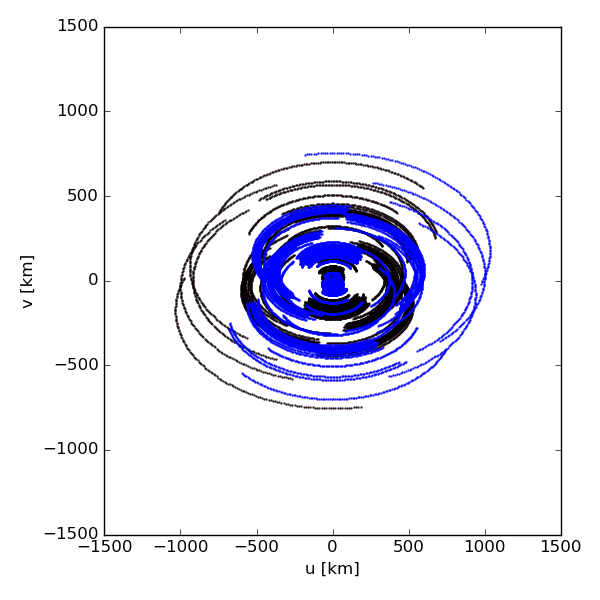
\includegraphics{images/lofar-uvcoverage-elsewhere.png}}
\caption{\label{fig.lofar.uvcoverage.elsewhere} $uv$-coverage of an 8-hour LOFAR observation when pointing 45 degrees away from zenith.}
\end{subfigure}
\caption{\label{fig.uvcoverage.lofar} Effect of array pointing on $uv$-coverage. By pointing the array 45 degrees in the $v$-axis, the array's $uv$-coverage (and thus maximum resolution) is decreased along the $v$-axis. Two colours are used, because $V_{AB}=V_{BA}$, and so only half the visibilities are stored in practice.}
\end{figure}


\subsection{The Point-Spread Function}\label{sec.imag.psf}

\pg
We have seen that the purpose an interferometric array is to overcome the diffraction limit of single-dish antennas. We have described visibilities, which are the quantities measured by an interferometric array. What remains is to describe how these measurements are related to the sky brightness distribution.

\pg
Assuming that all the antennas in an array are equivalent and perfectly calibrated, the van Cittert-Zernike theorem (\citetads{1934Phy.....1..201V}, covered in \citetads{2001isra.book.....T}) allows us to equate a visibility with a single Fourier mode of the plane tangent to the sky where the instrument is pointed. This direction is called the \emph{phase centre}, because phase shifts are introduced between antenna voltages before averaging so as to point each visibility in this direction. This behaviour is encoded in the Fourier kernel, which is written as:
\begin{equation}
k_p=2\pi i (( u_p l + v_p m + w_p (n-1) ))
\end{equation}



\pg
The Point-Spread Function (PSF) of an instrument is its point source response: it will determine the angular resolution limit due to the instrument. We know that the Fourier transform of a single point source with unit flux at phase centre is a constant. If we measured the full (infinite) visibility space, then we could reconstitute a point source perfectly. In practice, however, we only ever measure a subset of the visibility space: an interferometric array's PSF is thus the inverse Fourier transform of the array's $uv$-coverage, as these are the only points for which we have information on visibility space. The more elements in the array, the better the $uv$-coverage and thus the better the PSF. An interferometer's PSF will always be worse than an antenna dish of equivalent diameter, the UV-coverage of which is the inverse Fourier transform of a disc. This is because an interferometer behaves like a \emph{sparse} dish: the sparsity of our coverage manifests as very large point-spread function. The more baselines are available, the less sparse the UV-coverage, and so the better the PSF. This is shown in Fig. \ref{fig.vla.PSFvsUVcov}.

\pg
Mathematically, the $uv$-coverage of an interferometer can be treated as a series of delta functions centred on the antenna positions. To go from visibility space to image space, we apply the inverse Fourier transform, giving us:
\begin{align}
\mathbf{S}_{\mathrm{obs}} &= \mathcal{F}^*\left[ \mathbf{B} \sum_i^{n} \mathbf{x}_i \right]
\end{align}
where $\mathbf{S}_{\mathrm{obs}}$ is the observed sky brightness distribution, $\mathbf{B}$ the Fourier transform of the true sky brightness distribution $\mathbf{S}$, and $n$ is the number of antennas in our array. $\mathcal{F}^*$ is the inverse Fourier transform. By using the convolution theorem, we immediately see that
\begin{align}
\mathbf{S}_{\mathrm{obs}} &= \underbrace{\mathcal{F}^*\left[ \mathbf{B}\right]}_{=\mathbf{S}} \star \underbrace{\mathcal{F}^*\left[\sum_i^{n}\mathbf{x}_i \right]}_{\text{the PSF}}\\
\end{align}
and that our image is the convolution of the ``true", underlying sky brightness distribution, and our array's PSF. As $n \rightarrow \infty$, the $uv$-plane fills, and the inverse Fourier transform of this unit plane becomes 1. This illustrates the description above.

\begin{figure}[h!]
\centering
\resizebox{\hsize}{!}{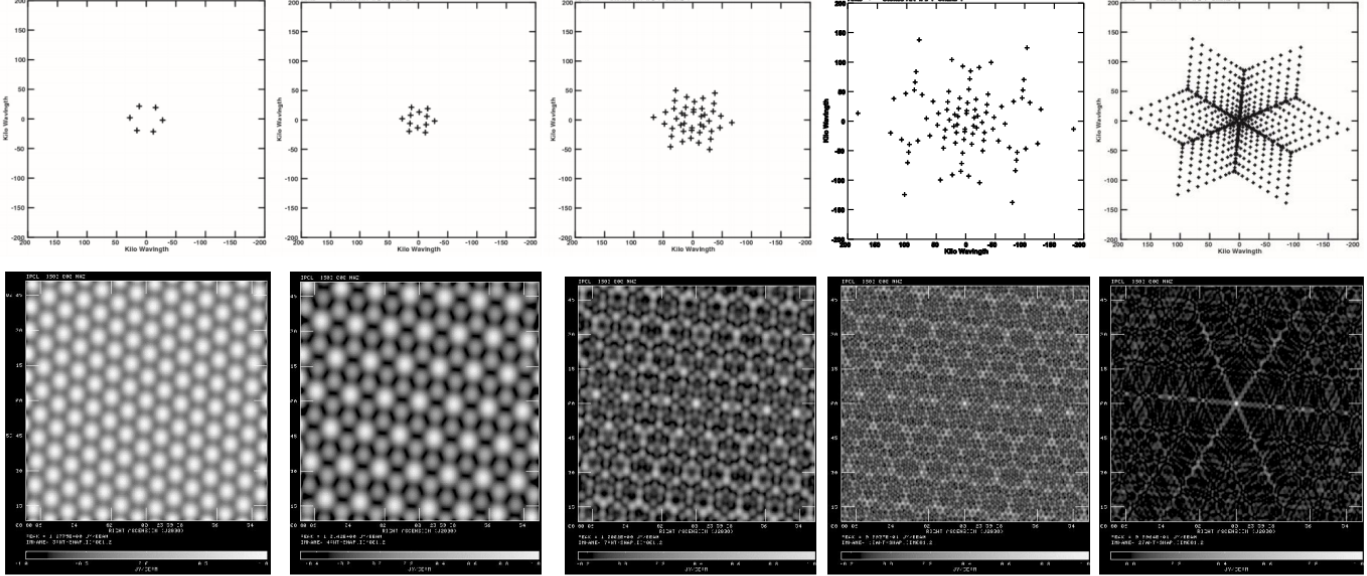
\includegraphics{images/PSFvsUVcov.png}}
\caption{\label{fig.vla.PSFvsUVcov}Plot of the PSF associated to more and more complete UV-coverage (here, consisting of more and more elements of the VLA). Image credit: Rick Perley, 3GC4 lecture.}
\end{figure}

\pg
This PSF can be improved by assuming that the sky is constant over periods of time (supersynthesis) or constant over fractions of the total bandwidth. This improves UV-coverage by a factor $N_\mathrm{t}\times N_\nu$, the number of measurements in time and frequency respectively. The effect of supersynthesis on the PSF is shown in Fig. \ref{fig.vla.PSFsupersynthesis}.
\begin{figure}[h!]
\centering
\resizebox{\hsize}{!}{\includegraphics{images/{PSF_supersynthesis}.png}}
\caption{\label{fig.vla.PSFsupersynthesis}Effect of supersynthesis on the UV-coverage of the full VLA. Image credit: Rick Perley, 3GC4 lecture.}
\end{figure}

\pg
Of course, even with these techniques, the PSF is never perfect, and flux from very bright sources will contaminate the rest of the field. The source in the last image of Fig. \ref{fig.vla.PSFsupersynthesis}, for example, only appears point-like by contrast to the others. If we wish to recover faint emission - and when interested in deep extragalactic fields, that is exactly what we wish to do - then we need to ensure that the effect of the PSF in our images is mitigated, for the brighter sources at least, lest their sidelobes (tails of the PSF convolved with the source) drown out signal from fainter sources. This means \emph{deconvolving} the PSF from radio interferometric images.

\subsection{From Dirty to Clean: Deconvolving the PSF}\label{section.clean}

\pg
Raw images made from radio interferometric data consist of the underlying flux distribution convolved to the array's PSF. The quantity of interest to astronomers is the underlying flux distribution. To recover that information from images, deconvolution is needed.

\pg
In practice, performing a full deconvolution on large images (easily over 25 million pixels in total) is not computationally viable. Scientists therefore resort to algorithms and techniques to accelerate imaging and deconvolution. For example, the use of Direct Fourier Transforms (DFT), which are extremely slow, is avoided when going from visibility space to image space - Fast Fourier Transforms (FFTs) are preferred. Similarly, one seeks to avoid having to perform full deconvolution on the dirty image, since many pixels in the image do not actually contain astrophysical signal. In this chapter, we will briefly cover the most common method of deconvolution used in radio astronomy.

\pg
We use dynamic range (DR) as a quality metric in radio images. DR is the ratio of the flux of the brightest source in the field to the flux of the faintest source in the field detectable above the noise. It is therefore a function of both source brightness and noise, and so we define dynamic range as:
\begin{equation}\label{eq.DR.imag}
DR = \frac{S_{max}}{\max(S_{min},\sigma)}
\end{equation}
where $S_{max}$ is the flux of the brightest source in the image, $S_{min}$ the flux of the faintest source detectable above the noise, and $\sigma$ is the noise in the image. The higher the DR, the deeper we image the sky, and thus the better the image. There are two big constraints to reckon with: firstly, we do not want to deconvolve the PSF from all pixels in the image, but only from those within which large amounts of underlying flux fall. Secondly, if we only deconvolve some pixels rather than performing a full deconvolution, then care must be taken not to treat artefacts in the field (which can be created from overlapping PSF sidelobes from neighbouring sources, even with perfect calibration) as true flux. Doing so would lead to an attempt to deconvolve a PSF from a pixel while assuming an incorrect underlying flux value for this pixel and thus result in the introduction of further artefacts in the image.


\pg
The dominant family of deconvolution algorithms used in radio astronomy at the time of writing is CLEAN\footnote{The other main family of deconvolution algorithms, Maximum Entropy Methods (MEM), are not very widely-used at the time of writing, but remain an active area of research (cf. \citetads{2018ApJ...857...23C}).} \citepads[see]{1974A&AS...15..417H,1984ARA&A..22...97P}, which is understood in compressed sensing theory as a matching-pursuit algorithm optimising L2 (i.e. a least-squares fit) with the addition of an L1 regularisation (i.e. the total flux in the model is minimised). The various CLEAN algorithms seek out the brightest pixel(s) in the image, potentially applying a mask to the image first in cases where some \emph{a priori} knowledge on flux distribution is available. It then deconvolves those pixels up to a predefined threshold (either a fraction of the initial pixel value or some factor of the estimated noise value). It does this some predefined number of times. Then, it collects the aggregate \emph{model} (the flux estimate for each deconvolved pixel up to this point), convolves the model with the PSF, and subtracts the result from the dirty image. It then begins to choose the brightest pixels again, and continues to clean until it reaches a stopping condition (usually either a flux value or a maximum number of iterations).

\begin{figure}[h!]
\centering
\resizebox{\hsize}{!}{\includegraphics{images/{dirty-vs-clean}.png}}
\caption{\label{fig.vla.clean} Effect of deconvolution on a dirty image of 3C295. To the left, the dirty image; to the right, the deconvolved image (same size, resolution \& flux scale, made with the same data). As we can see, the latter is much more scientifically interesting.}
\end{figure}


\pg
In Fig. \ref{fig.vla.clean}, we show the effect of deconvolution on a dirty image of 3C295 (a very bright \& complex source which is the subject of much of this thesis' work). Since this source includes diffuse emission, standard CLEAN is insufficient (since CLEAN assumes a sparse distribution of point-like sources). Instead, the DDFacet software package's novel SSD/GA algorithm (see \citetads{2017arXiv171202078T}), which deconvolves islands consisting of sets of pixels at once, was used. This allowed for a far greater dynamic range than standard CLEAN could achieve, while also more properly recovering diffuse emission: when imaging a resolved source, this is absolutely necessary.

\pg
The problem of imaging radio interferometric data is still a very active field of research today. For more information on this topic, the NRAO website\footnote{See \href{https://www.cv.nrao.edu/~abridle/deconvol/node8.html\#SECTION00051000000000000000}{the CLEAN section of the NRAO website}.} is an excellent start for a general introduction to this topic, while \citet{2017arXiv171202078T} provides an outstanding example of cutting-edge work at the time of writing.

\section{Unifying Calibration \& Imaging}\label{sec.CalibImagery}

\pg
The previous section mentions that good deconvolution is dependent on good calibration: poor calibration introduces artefacts in images, which can in turn bias deconvolution. A wrong model of the sky brightness distribution, in turn, will bias calibration, introducing artefacts in images. This feedback of one inverse problem onto the other is a strong indication that both are, in fact, different facets of the same underlying inverse problem: going from measured visibilities to a sky brightness distribution. Indeed, one could - conceptually, at least - solve for both problems at once: find both the sky brightness distribution and the antenna gains which best fit the measured visibilities. In practice, this is not practical (though it is feasible); not only is there no proof that the overall calibration \& imaging problem is convex, but even if it is, it is also poorly conditioned: multiple sets of sky brightness distributions \& antenna gains are equally viable for a given set of measured visibilities. This means that, even if the problem is convex, it takes an extremely long time to converge properly. Examples of convexity and conditioning are shown in \cref{fig.examples}.

\begin{figure}[h!]
\centering
\begin{subfigure}{.32\textwidth}
\resizebox{\hsize}{!}{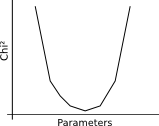
\includegraphics{images/GoodConditioning.png}}
\caption{\label{fig.goodconditioning} Convex, Well-conditioned}
\end{subfigure}
\hfill
\begin{subfigure}{.32\textwidth}
\resizebox{\hsize}{!}{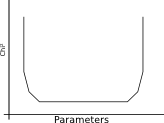
\includegraphics{images/BadConditioning.png}}
\caption{\label{fig.badconditioning} Convex, ill-conditioned}
\end{subfigure}
\hfill
\begin{subfigure}{.32\textwidth}
\resizebox{\hsize}{!}{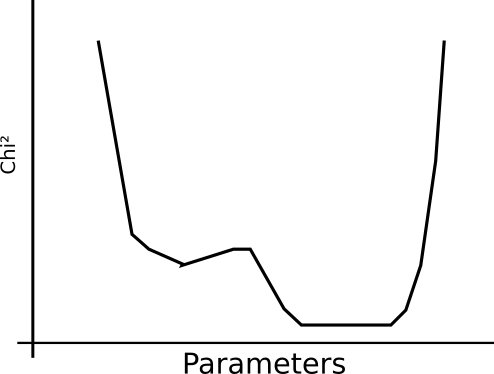
\includegraphics{images/NotConvex.png}}
\caption{\label{fig.notconvex} Non-convex, ill-conditioned}
\end{subfigure}
\caption{\label{fig.examples} Examples of poor conditioning and non-convexity, plotted in terms of residual $\chi^2$ values vs parameter values.  Note that all the parameters of our problem are collapsed onto a single axis and treated as a scalar: this is for illustrative purposes. Note that the local minimum of the non-convex example is well-conditioned while its global minimum is ill-conditioned.}
\end{figure}

\pg
Bad conditioning and non-convexity can be alleviated through regularisation: by specifying a well-chosen prior (e.g. for interferometry, using a good sky model for calibration), the underlying distribution of the solutions can be constrained to fall in a narrow, convex region. This is shown in \cref{fig.selfcal.regularise}
\begin{figure}[h!]
	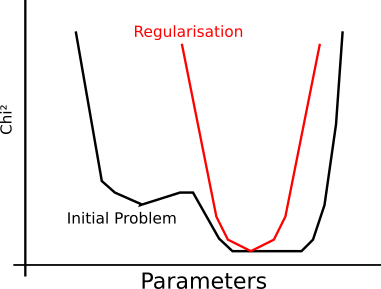
\includegraphics[width=.6\linewidth]{images/regularise.png}
	\caption{\label{fig.selfcal.regularise} Plot showing the effect of regularisation on an ill-conditioned, non-convex problem. The $\chi^2$ fit is constrained to lie in a convex, well-conditioned region: it falls within the global minimum, at at one point only rather than somewhere in a valley.}
\end{figure}

\pg
Because the imaging problem (i.e. the problem of deconvolution) is linear, it can only be convex - though it is not necessarily well-conditioned. As for the calibration problem, experience strongly indicates that it is nearly convex \textit{and} ill-conditioned. For calibration convexity, Cyril Tasse (pers. comm.) has found that the Hessian matrix of the gain solutions is positive semidefinite, i.e. that all its eigenvalues are positive and non-zero except for one. This behaviour likely explains why self-calibration is, in the practical experience of radio-interferometric practicioners,  neither well-conditioned nor convex: if the problem is poorly regularised, then the same initial model may give different end results, and to truly verify the convergence property of self-calibration would require both a full Monte Carlo simulation and enough time to allow the very slowly-converging procedures to finish converging. It is not a practical thing to test rigorously.

\pg
Because the net calibration \& imaging problem has so many degrees of freedom, it is convenient to break it into two parts: calibration and imaging. By doing this, instead of exploring a massive set of hyperparameters (e.g. relative flux distribution at a given frequency, overall spectral index, the 8 values of a complex $2\times 2$ matrix per antenna per time and frequency interval, ...), a smaller subset of these hyperparameters is explored while all else is kept constant. By ensuring that these subsets each give reasonable results individually, it becomes possible to solve the full problem. This practice of imposing specific priors to each subset of the problem is a form of regularisation: it can turn a poorly-conditioned problem into a better-conditioned one, provided that the priors are well-chosen.

\pg
In effect, this means going from exploring the sky-gains parameter space all at once to exploring it along one ``axis\footnote{which includes all the hyperparameters associated with that subset of the problem}" at a time. This is illustrated in \cref{fig.selfcal.paramexplore}. 
\begin{figure}[h!]
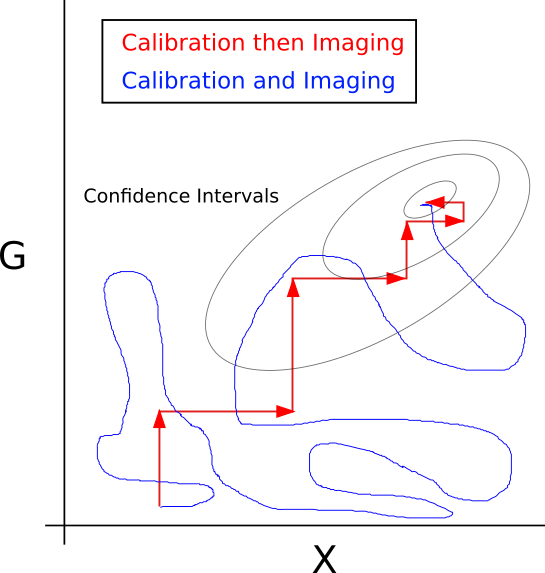
\includegraphics[width=.6\linewidth]{images/Selfcal-paramExplore.png}
\caption{\label{fig.selfcal.paramexplore} Plot showing the exploration of sky-gains (X-G) parameter space. In red, this space is explored one axis at a time (this is ``self-calibration"); in blue, the full space explored at once. Here, we show both procedures converging to the best confidence value: in practice, this is rarely the case.}
\end{figure}

\pg
In this context, a good deconvolution algorithm is one that is able to minimise how much it is affected by calibration errors while maximising how much true underlying flux it can recover into a model, while a good calibration algorithm is one that is able to minimise how much it is affected by sky model errors while maximising how much true underlying gain structure it can recover.



\section{Weighting Schemes}
\pg
We will finish our introduction to the inverse problem of interferometry by discussing one method by which the conditioning of deconvolution can be improved. Consider two extreme cases: a field containing a few point sources(\cref{fig.point}), and a field containing a diffuse and turbulent source, with very complex flux distribution at all scales (\cref{fig.cyga}). Deconvolving the PSF from the first image using CLEAN algorithms will be child's play, but doing the same with the second will be extremely complex. The first case is well-conditioned, and the second to ill-conditioned.

\begin{figure}[h!]
\centering
\begin{subfigure}{.45\textwidth}\resizebox{\hsize}{!}{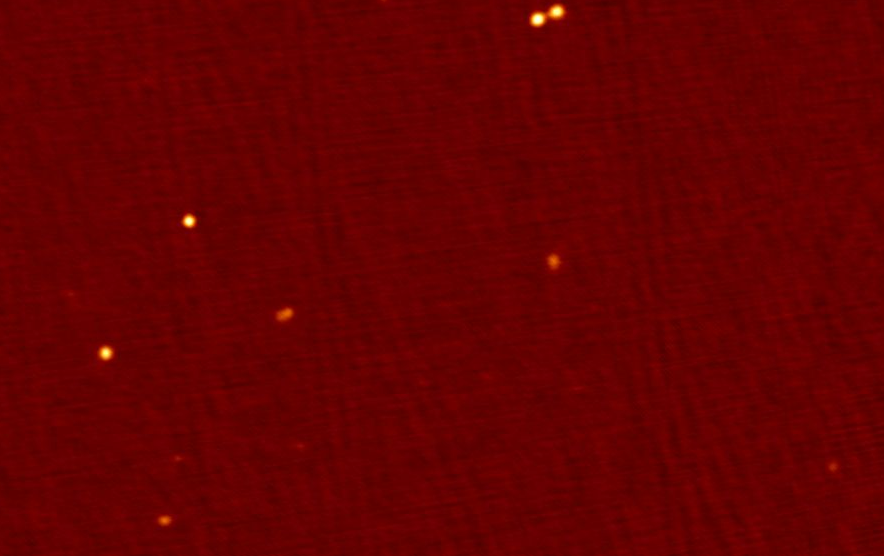
\includegraphics{images/egs-prelim.png}}
\caption{\label{fig.point} Part of the LOFAR field near the Extended Groth Strip as seen by LOFAR.}
\end{subfigure}
\hfill
\begin{subfigure}{.53\textwidth}
\resizebox{\hsize}{!}{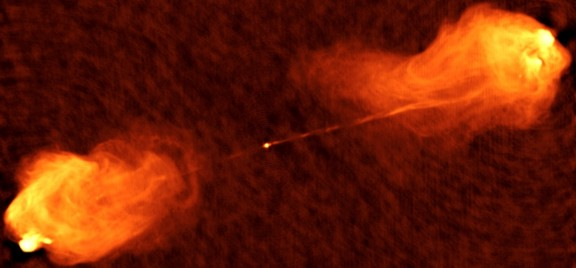
\includegraphics{images/cyga.jpg}}
\caption{\label{fig.cyga} Cygnus A as seen by the VLA. \href{http://images.nrao.edu/110}{Image courtesy of NRAO/AUI}}
\end{subfigure}
\caption{\label{fig.conditioning} Two extreme examples of good and poor conditioning. \cref{fig.point} shows a field with a few point-like sources. \cref{fig.cyga} shows a very complex \& diffuse structure.}
\end{figure}

\pg
The better the conditioning, the easier the deconvolution and the closer to the ground truth its result. As such, when the true underlying structure of a source is poorly-known, getting the best conditioning possible for deconvolution becomes a key concern. Thankfully, because the actual measurements taken with interferometers are the Fourier modes of the sky brightness distribution, they can be weighted when reconstructing the images to fulfill specific requirements. In particular, Briggs weighting \citepads{1995AAS...18711202B} gives a sliding parameter between \emph{natural} weighting, where each visibility is weighed equivalently (this optimises noise in the field) and \emph{uniform} weighting, which gives each visibility a weight inversely proportional to $uv$-plane density. Uniform weighting optimises for resolution at the cost of image signal-to-noise.

\begin{figure}[h!]
\centering
\begin{subfigure}{.48\textwidth}\resizebox{\hsize}{!}{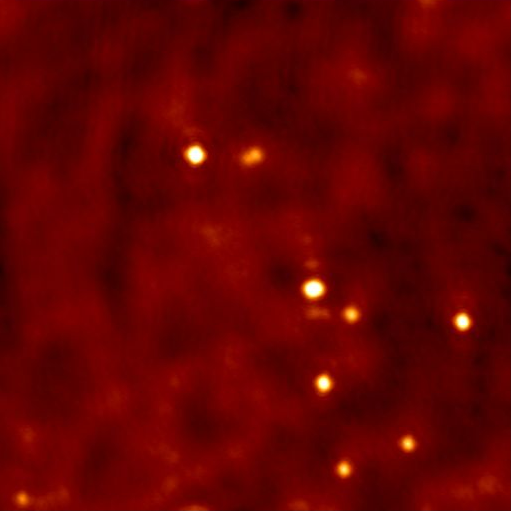
\includegraphics{images/natural.png}}
\caption{\label{fig.natural} Image made with LOFAR data and natural weighting.}
\end{subfigure}
\hfill
\begin{subfigure}{.48\textwidth}
\resizebox{\hsize}{!}{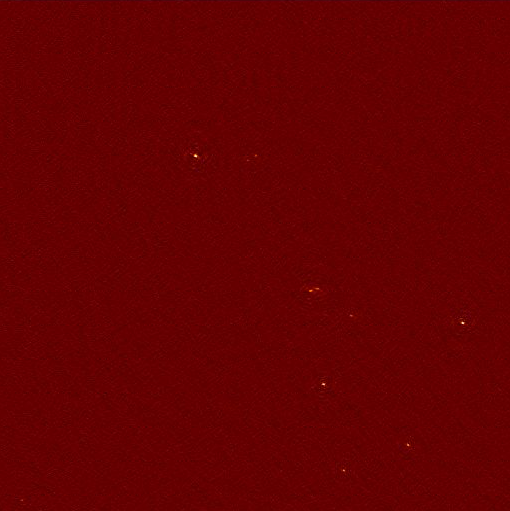
\includegraphics{images/uniform.png}}
\caption{\label{fig.uniform} Image made with the same data as \cref{fig.natural} and uniform weighting.}
\end{subfigure}
\hfill
\begin{subfigure}{.48\textwidth}
\resizebox{\hsize}{!}{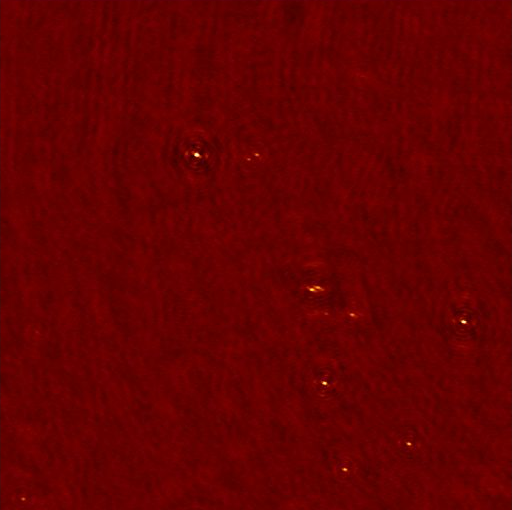
\includegraphics{images/briggs0.png}}
\caption{\label{fig.briggs0} Image made with the same data as \cref{fig.natural} and Briggs weighting, with a Briggs parameter of 0.}
\end{subfigure}
\caption{\label{fig.briggs-weighting}Impact of different weighting schemes on interferometric image reconstruction. All the images shown above are deconvolved.}
\end{figure}

\pg
\cref{fig.briggs-weighting} shows images done with the same data and the same imaging parameters bar weighting scheme choice. We can see that different weighting schemes give radically different deconvolved images. Images made with uniform (\cref{fig.uniform}) or Briggs (\cref{fig.briggs0}) weighing are much sharper, with uniform weighting (\cref{fig.uniform}) giving such resolution that the sources are nearly invisible in the field (though they are present - the contrast was not upped so as to show all three images on the same flux scale). 

\pg
%Note that the weighting schemes shown here rely only on a choice between normalising visibilities by local $uv$-density vs. signal-to-noise, with Briggs weighting providing a formal method for going from one regime to another or optimising between both. Other weighting schemes exist - one can attempt to optimise data size vs decorrelation\footnote{As data is averaged, decorrelation becomes more and more important in the field. See \cref{section.RIME} for more details.}, for example \citepads[see]{2016MNRAS.462.2542A}. This can help ensure a homogeneous conditioning of the deconvolution problem in the image, by ensuring that the PSF is as peaked as possible throughout the field of interest. Part of the work of this thesis was in devising a weighting scheme dependent on calibration quality, to drastically improve deconvolution conditioning and final image quality. This weighting scheme is described in much greater detail in \cref{chapter.paper}.

\pg
We close this section by noting that data flagging can be considered a form of weighting scheme. This consists of assigning a null weight to those data points considered too corrupted by various instrumental or atmospheric effects (typically, Radio Frequency Interference - RFI - cf. \citetads[cf.]{2010ascl.soft10017O} for an example) to be scientifically useful. Those weights which are deemed too corrupted are assigned a weight of zero. This corresponds to simply dropping those data points which would corrupt the image reconstruction by introducing unphysically strong fringes in the image.

\pg
Flagging is also useful to remove corrected visibilities for which near-zero gains are found: the associated corrected visibilities will consist of some number divided by a near-zero number, for which numerical errors can introduce very large errors. ``Clipping" these visibilities after calibration helps improve the final images.

\section{An Observer's Perspective of Radio Interferometry}

\pg
Astronomers who request observation time on interferometric arrays are generally not experts in the theory and operation of these arrays. This is a simple consequence of scientific division of labour. This thesis is written from the perspective of an ``expert" user: one who specialises in understanding interferometric arrays and reducing their data, rather than their subsequent analysis. However, it can be very helpful to contextualise this perspective in the experience of other scientists, which is what this section aims to do. This is simply to highlight the conceptual structure of a radio interferometric observation, and where the concepts outlined in this chapter fall in the overall pattern. In other words, it is best understood as a guide to see where a given section's topic slots into the overall production of an image made from visibilities.

\pg
LOFAR data can be acquired through observation or via the Long-Term Archive. The worst of this data will already be flagged. Users can thus generally proceed directly to calibration. Because there is no guarantee of sufficient signal-to-noise in the ``target field" (the object that the astronomer is actually interested in), it is standard practice to observe a calibrator source for 5 minutes before and after each observation. Such sources typically need to be bright and unresolved for the interferometer being used. Because they are bright and at phase centre for the 5-minute observation, the SNR when solving for calibration solutions for these 5 minutes will tend to be quite good. These solutions will then be interpolated between the 5 minutes onto the 8-hour observation. Calibration will be described in \cref{section.calibration}.

\pg
So far, the astronomer will have worked entirely with visibilities. However, generally speaking, the aim will be to get information on the object's spatial brightness distribution at the observing frequency. This will require \emph{imaging}: going from visibilities to the image-plane. This can be done through a variety of tools, but will generally involve deconvolution. Imaging will be the subject of the rest of this chapter, and deconvolution will be described in more detail in \cref{section.clean}.

\pg
After obtaining the initial image, it may be desirable to perform a few rounds of self-calibration \citepads[cf.]{2018arXiv180505266B} on the target field. This consists of extracting a model from the initial image and using it as a new calibration model, then re-imaging. Doing this will usually dramatically improve the final image. 

\pg
The framework for interferometric calibration is complex, and understanding it requires a good grasp on interferometry itself. For now, we will assume that calibration has been performed perfectly, and that the gain-corrections have been applied to the voltage measured by our antennas. We therefore work with the true signal from astrophysical sources until \cref{section.RIME}.
\clearpage
% !TeX spellcheck = en_UK

\section{Calibration Methods in Radio Interferometry}\label{section.calibration}
\pg
In this section, we will discuss the implementation of interferometric array calibration. Our analysis is based on the RIME formalism, described in \cref{section.RIME}. One key metric of calibration quality is the \emph{dynamic range}, mentioned in Sec. \ref{section.clean}. High dynamic ranges mean that a high contrast has been obtained, and fainter sources can be reached. Here, because the difference between thermal noise and artefacts becomes relevant, we redefine dynamic range as follows
\begin{equation}\label{eq.DR}
DR = \frac{S_{max}}{S_{min},\max(\sigma_{thermal},\sigma_{artefacts})}
\end{equation}
where $S_{max}$ is the flux of the brightest source, $S_{min}$ the flux of the faintest source detectable above the noise, $\sigma_{thermal}$ the thermal noise in the image, and $\sigma_{artefacts}$ the noise associated with calibration artefacts. This gives a definition for dynamic range useful even in fields with a single source. We can thus use it as a metric for calibration quality specifically.

\pg
The distinction between these two noise sources is crucial; one can never go `below noise' for a given observation, no matter the quality of calibration. Astronomers typically observe for longer periods of time in order to reduce $\sigma_{thermal}$ in their images, but this will not reduce the artefacts caused by poor calibration solutions. Uncorrected Direction-Dependent Effects\footnote{See \cref{section.RIME.MultiplePointSources}} will not go away on their own, no matter how long the integration time. Similarly, there is a limit to how much improving calibration will improve the final image: eventually, more data is required to drive noise down.

\pg
We can distinguish three `generations' of calibration methods, of increasing complexity \citepads{2010A&A...524A..61N}. We will describe them in terms of the RIME, showing how each generation increases in generality to account for more exotic effects. They are referred to interchangeably as `nth-generation calibration' or `nGC' methods.

\subsection{Generational Analysis}

\subsubsection{First-Generation: Open-Loop Calibration}\label{section.calibration.1gc}

\pg
First-generation calibration methods (1GC methods) consist of open-loop calibration. This relies entirely on instrument stability, and thus imposes significant design constraints on radio telescopes. It consists of briefly observing an external calibrator before and after each observation run to find calibration solutions for those calibrator observations, and then interpolate between them over the ``target" observation. %\footnote{For a concrete example, see \href{http://www.analog.com/en/analog-dialogue/articles/open-loop-calibration-techniques.html}{the open-loop calibration techniques page of analog.com}.}
%\pg
%Phase calibration in the 1GC era `proper' was not necessary, as engineers were capable of ensuring adequate phase stability in contemporary interferometers. Phase was thus calculated relative to a fixed frame of reference, usually the central antenna of a 3-antenna array. 
In RIME terms (see \cref{section.RIME}), this consists of solving for a very basic form of $\Gjones_p$:
\begin{equation}
\Gjones_p = a_p \bm{\mathrm{I}} % \begin{bmatrix} e^{2 \pi i \nu ( \phi_p - \phi_0)} \end{bmatrix}
\end{equation}
where $a_p$ is a complex constant solved for during open-loop calibration. By interpolating between the two calibrator observations, it is possible to have a linear time-dependent gain estimate, though it is not much more complex than the above. %, $\nu$ the observing frequency, $\phi$ the phase at an antenna, and $\phi_0$ the phase at the reference antenna.

\pg
While values for $a_p$ and $b_p$ can in theory be found for both autocorrelation and both crosscorrelations (e.g. XY and YX for linear receptors), low signal-to-noise means that in practice, a single set of values is solved for per antenna\footnote{This reduces calibration to solving only for the intensity gains: the data can then only be used for \emph{intensity mapping} (e.g. \citepads{1957IAUS....4..159J}). This practice therefore precludes polarimetry.}. With these techniques, one can achieve dynamic ranges of about 100:1 (\citepads{2010A&A...524A..61N}).

\subsubsection{Second-Generation: Self-Calibration}\label{section.calibration.2gc}

\pg
Second-generation calibration methods (2GC methods) are defined by \emph{self-calibration}\footnote{On the discovery of self-calibration and its evolution in parallel to adaptive optics, see the chapter titled "The Almost Serendipitous Discovery of Self-Calibration'' in "\href{http://library.nrao.edu/public/collection/02000000000280.pdf}{\citep{serendipitous}}.}, commonly referred to as \emph{self-cal} (\citepads{1984ARA&A..22...97P}). As described in \cref{section.RIME.FullSky.CVZ}, this method can only be deployed if the brightness matrix of the sky is the same for all baselines\footnote{This is not to say that the brightness matrix must contain only point sources, but rather that moving our interferometer 500m to the East should not change its measured visibilities} (i.e. that we are not affected by direction-dependent effects).

\pg
The first instance of self-calibration (and adaptive optics in radio interferometry) is a paper published in the era of 1GC by Jennison \citepads{1958MNRAS.118..276J}, expanding on his PhD work, which was published in 1951). With sufficient signal-to-noise, he showed that \emph{phase closure} could be calculated and errors due to the atmosphere thus mitigated.

\pg
Self-calibration and adaptive optics are essentially the same thing, albeit meeting different constraints. Most notably, interferometric data is digital, allowing radio astronomers to perform their adaptive optics correction after the observation.

\pg
If amplitude and phase gains can be written as antenna-dependent, then each antenna-based error is estimated N times (once per each baseline which includes this antenna). By estimating, and correcting for, these errors, one can use a simple source model to infer an improved one. This is why the method is referred to as self-cal; by calibrating `on' a good calibrator source (bright, compact and unresolved), one can drastically improve one's source model, along with one's calibration solutions.


\begin{figure}[h!]
\centering
\resizebox{\hsize}{!}{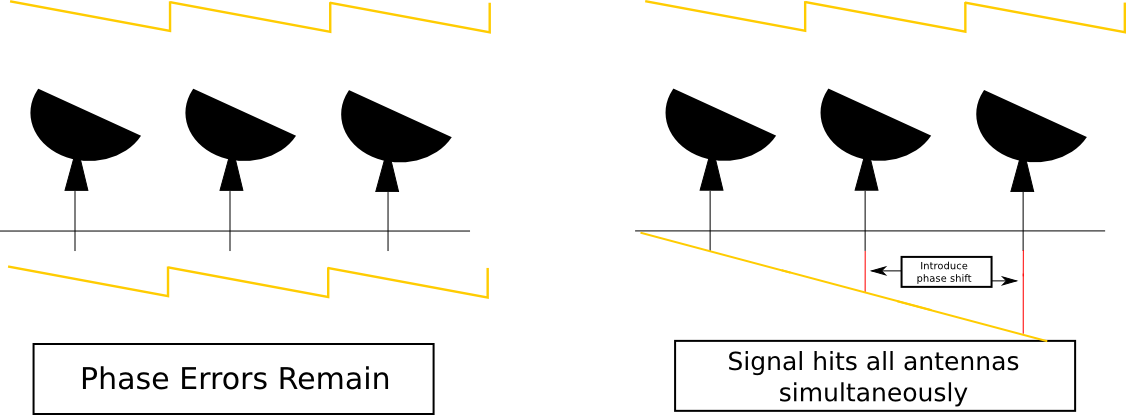
\includegraphics{images/selfcal.png}}
\caption{\label{fig.selfcal} Representation of self-calibration as adaptive optics}
\end{figure}

\pg
By extending this idea to VLBI (see e.g.  \citepads{1974ApJ...193..293R}), \emph{amplitude closure} was introduced to the field along with phase closure \citepads[as described in][]{1983Sci...219...51R}. These quantities are immune to antenna-based effects.%Astronomers were quick to apply these methods to interferometers in general.

\pg
The great advantage of radio interferometry over optics, however, is that we can \emph{iterate} over progressively improved source models. This is because interferometric data is digital, and because we record phase information.

\pg
In practice, of course, self-cal will be limited by noise. More precisely, it will be limited by two factors: sensitivity, in the form of the signal-to-noise ratio (henceforth SNR), and the atmosphere (as sufficient SNR is needed per coherence time, which is a function of atmosphere activity). For sufficiently bright sources, with high SNR, self-calibration can easily improve dynamic range by a factor of 10 (\cite{serendipitous}, p. 154) in a single iteration. 

\subsubsection{Third-Generation: Direction-Dependent Effects}

\pg
Third-generation calibration (3GC) is an extension of 2GC calibration which takes direction-dependent effects into account. At the time of writing, this is the cutting edge in radio interferometric calibration.

\pg
In this section, I will discuss the \emph{facet-based} approach taken by \citetads{2017arXiv171202078T}. The approach cannot be divorced from imaging, for the simple reason that solving for and applying Jones matrices\footnote{See \cref{section.RIME} for a full discussion on calibration and Jones matrices} in different directions requires image-plane knowledge of the sky brightness distribution $\Bmatrix$. % The imaging challenges this methods introduces will be discussed in [href to relevant imaging section].

\begin{figure}[ht]
\centering
\resizebox{\hsize}{!}{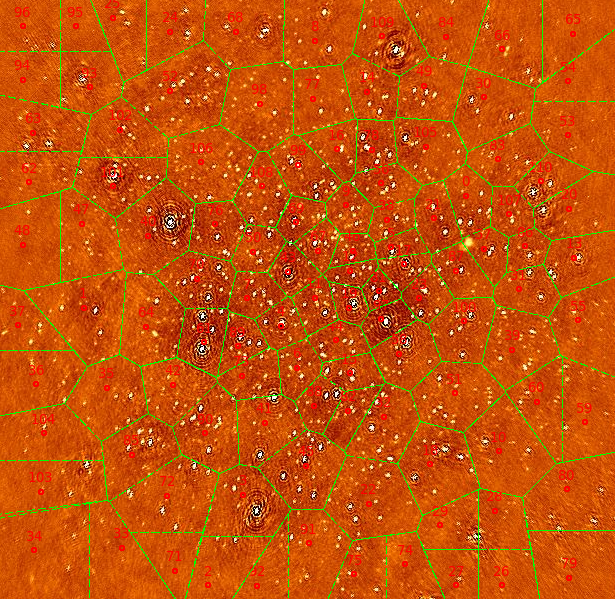
\includegraphics{images/bootes-image.png}}
\caption{\label{fig.facets} Voronoi facets, as implemented in DDFacet. Image is made before application of direction-dependent correction. This is an image of the Bootes field, made by Cyril Tasse.}
\end{figure}

\pg
When performing first and second-generation calibration, one solves for a set of Jones matrices or parameters thereof. Direction-independent calibration then consists of applying these calibration solutions to the visibilities directly. However, while these solutions will be correct in the direction of the calibrator source, they are increasingly likely to be wrong as a function of distance from said calibrator source. The difference between the true gains in a given direction and the gains estimated from the calibrator source are called \emph{differential gains}.

\pg
Why then not solve for a set of calibration solutions for each source in the calibration model, iteratively adding new sources to this model as they become above the noise as calibration artefacts - introduced by poor calibration - decrease? There are two main reasons for this: firstly, the SNR when calibrating using very faint source models will be poor. This means that gains will likely be extremely noisy, and applying them will result in increased calibration artefacts in the final image. Secondly, even by optimising for signal-to-noise and only using a few of the brightest sources in the field, the problem quickly becomes intractably large in terms of computing power required, provided that standard complex differentiation is used \citepads[see][]{2016ApJS..223....2V}. Wirtinger differentiation \citepads[see][]{2014arXiv1410.8706T,2015MNRAS.449.2668S} does alleviate this somewhat by allowing the Hessian matrix to be written as a block-diagonal matrix, but is not implemented in all standard direction-dependent calibration software at the time of writing.

\pg
The crucial insight of a faceting approach is then to split the image into a set of \emph{facets}, solving for a set of calibration solutions for each of these facets. These solutions are then applied to the visibilities when mapping them onto the dirty image. The faceting in DDF is shown in \cref{fig.facets}. The facet distribution shown in \cref{fig.facets} encourages an even flux distribution in multiple facets, and ensures that no facet is so small that too little signal would be available within. As we can see from \cref{fig.DDcal.effect}, direction-dependent calibration can drastically improve the quality of wide-field images. It currently represents the state of the art in interferometric calibration. 

\begin{figure}[h!]
\centering
\begin{subfigure}{\textwidth}
\resizebox{\hsize}{!}{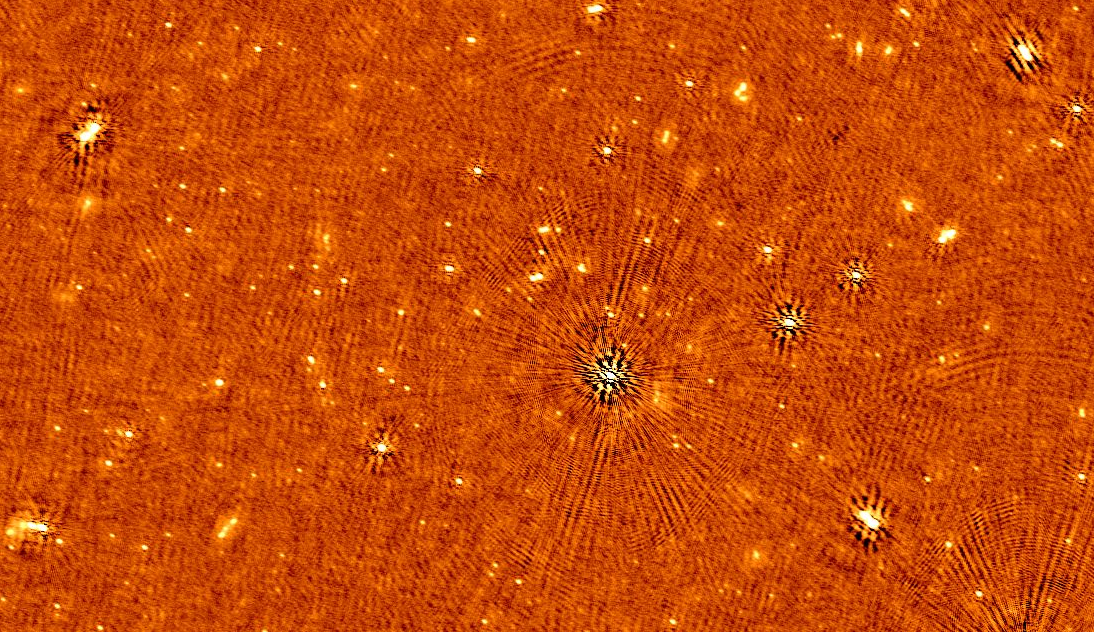
\includegraphics{images/lofar-nocorr.png}}
\caption{\label{fig.lofar.noDDcal} Image of the Boötes field, made without direction-dependent calibration. Image by Cyril Tasse.}
\end{subfigure}
\begin{subfigure}{\textwidth}
\resizebox{\hsize}{!}{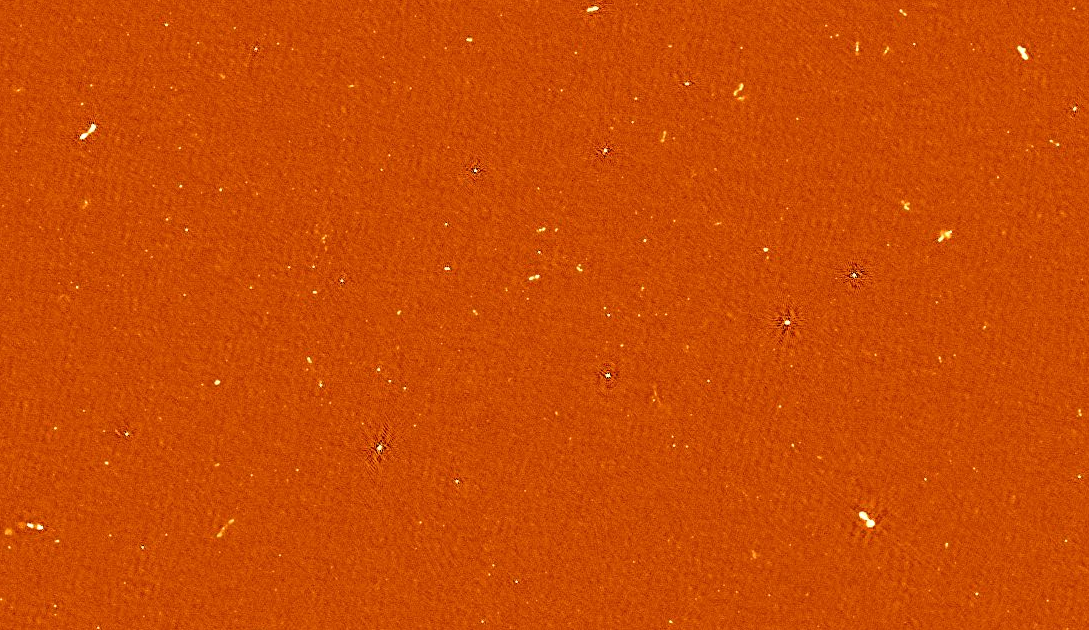
\includegraphics{images/lofar-corr.png}}
\caption{\label{fig.lofar.withDDcal} Image of the same Boötes field, made with direction-dependent calibration. Image by Cyril Tasse.}
\end{subfigure}
%\hfill
\caption{\label{fig.DDcal.effect} Difference between imaging made with (Fig. \ref{fig.lofar.withDDcal})and without (Fig. \ref{fig.lofar.noDDcal}) third-generation calibration.}
\end{figure}








\clearpage
% !TeX spellcheck = en_UK

\section{The RIME Formalism}\label{section.RIME}
%\minitoc

\pg
In this section, we introduce the mathematical framework which forms the basis for our algorithmic work.
While radio interferometry has historically been a complex business \citepads{2001isra.book.....T}, modern radio interferometry is based on the Radio Interferometer's Measurement Equation, a powerful and elegant formalism which underpins modern calibration and imaging algorithms. In this section, I will give a simplified account of this formalism as described in \citetads{2011A&A...527A.106S} and its companion papers \citepads{2011A&A...527A.107S, 2011A&A...527A.108S, 2011A&A...531A.159S}. This will form the theoretical basis on which further sections will expand.% I cannot overstate the importance of the RIME as the foundation of modern calibration and imaging algorithms.

\pg
For a mathematically rigorous description of the RIME, the references used in this work (particularly \citetads{2011A&A...527A.108S} and \citetads{2011A&A...531A.159S}) are obviously the first place to look. We frame the RIME in the continuity of previous theoretical frameworks of radio interferometry, while also describing it in the context of contemporary software packages and algorithmic tools.

\section{Setting up the RIME: a single point source}
\label{section.RIME.setup}

\pg
The Radio Interferometer's Measurement Equation, or RIME, is a formalism which allows for an elegant and efficient formulation of the physical processes which affect signal propagation, from astrophysical effects to instrumental effects. Its fundamental underlying hypothesis is \emph{linearity}: that transformations along the signal are linear with respect to the basis chosen to represent our signal. In other words, this means assuming that propagation effects are separable by antenna.

\pg
Consider a single quasi-monochromatic point source in the sky. Its signal at a point in time and space can be described by a complex 2-vector $\evector$ -- this assumes plane waves. We can then represent physical processes which affect this signal's propagation using \emph{Jones matrices}. In other words:
\begin{align}
\volt &= \Jones\evector\\
\evector &= \begin{pmatrix} e_x \\ e_y \\ e_z \end{pmatrix}
\end{align}
where $\volt$ is the voltage measured by our antenna, and $\Jones$ the Jones matrix describing the \emph{net} propagation effects - atmospheric, astrophysical, and instrumental - which affect our source's signal. $\evector$ is the electromagnetic wave emitted by a source. $\Jones$ can be written as a series of matrix products, each individual matrix describing a physical phenomenon. They are then called a \emph{Jones chain}, and the resulting $\Jones$ is often called the \emph{total Jones matrix}.

\pg
For $\mathbf{e}$ to be a 2-vector, rather than a 3-vector, we must choose to use $xyz$ as our coordinates, with $z$ the direction of propagation of our signal. \citetads{1996A&AS..117..137H} then show that the following relation holds:
\begin{equation}
2 \evector \evector^\Herm = 2  \begin{bmatrix} <e_x e_x^\star> & <e_x e_y^\star> \\ <e_y e_x^\star> & <e_y e_y^\star> \end{bmatrix} = \begin{bmatrix} I+Q & U+iV \\ U-iV & I-Q \end{bmatrix} = \Bmatrix
\end{equation}
where $\Bmatrix$ is the coherency matrix of the source's emission.

\pg
A visibility is the correlation of voltage from two antennas. In other words,
\begin{align}
\Vis_{pq} &= 2 \langle\volt_p (\volt_q)^\Herm\rangle\\
\Vis_{pq} &= 2 \langle\Jones_p \evector (\Jones_q \evector)^\Herm\rangle\\
\Vis_{pq} &= 2 \langle\Jones_p \evector \evector^\Herm \Jones_q^\Herm\rangle
\end{align}
where $\Jones_p$ corresponds to the signal propagation chain of antenna $p$, and $\Jones_q$ for antenna $q$. $(...)^\Herm$ corresponds to taking the Hermitian conjugate of a matrix, and $\langle...\rangle$ an average over some interval. Note that a factor of 2 has been introduced here, as a matter of convention. This is due to the definition of the Stokes parameter in relation to our $\evector$ outer product.



\pg
We can thus write:
\begin{equation}
\Vis_{pq} = \Jones_p \Bmatrix \Jones_q^\Herm
\end{equation}

\pg
This gives us an elegant formulation of the relationship between the signal emitted by an astrophysical source and its corresponding measured visibility. The Stokes parameters\footnote{Stokes parameters determine the polarisation of light; we will not get into more details in this manuscript, as it is hardly relevant to the topic at hand. Suffice to say that the 2-vector formalism helps account for the polarised nature of light.} of our source can be directly calculated from our measured visibility, provided $\Jones_p$ and $\Jones_q$ are known. Of course, in practice, they are not, and must therefore be modelled. To do this, we must expand each Jones matrix into a corresponding Jones chain.

\section{Expanding our Jones Chain}
\label{section.RIME.JonesChain}
\pg
Having written our RIME as a matrix multiplication problem, we can now begin to differentiate between different types of Jones matrices. $\Jones_p$ describes the \emph{aggregate} effects which occur over the course of the signal's propagation to our antenna $p$. It can be split into a Jones chain of $n$ separate matrices, corresponding to different effects:
\begin{align}
\displaystyle \Jones_{sp}^H &= \prod_1^n \Jones_{nsp}^H = \Jones_{1sp}^H \Jones_{2sp}^H ... \Jones_{nsp}^H\label{eatshit1}\\
\displaystyle \Jones_{sp}   &= \Jones_{nsp}...\Jones_{2sp} \Jones_{1sp}\label{eatshit2}
\end{align}
where $s$ is a particular direction in the sky: these Jones matrices are therefore direction-dependent. Going from \cref{eatshit1} to \cref{eatshit2} simply consists of applying the Hermitian operator to both sides of \cref{eatshit1} to recover $\Jones_{nsp}$.
Since the Jones terms are applied sequentially to the brightness matrix, starting with $\Jones_{1sp}$, the terms to the right of our decomposition of $\Jones_{sp}$ can be said to occur `at the source', i.e. before those to the left (said to occur `at the antenna').

\pg
Our aim is thus to find the Jones chain which most concisely describes the different \emph{types} of effects affecting our signal. In order of increasing complexity, there are three: so-called \emph{geometric} effects, \emph{direction-independent} effects, and \emph{direction-dependent} effects.

\subsection{Geometric Effects: the Phase Delay Jones Matrix}
\label{section.RIME.JonesChain.Kjones}

\pg
The physical quantity measured by an interferometric array, the \emph{visibility}, is not a function of the absolute phase of our signal, but rather a function of the \emph{phase difference} between our measured voltages $\volt_p$ and $\volt_q$. In other words, it is a function of the phase difference on \emph{baseline} $pq$, which consists of antennas $p$ and $q$. The direction which minimises this difference is called the \emph{phase centre}\footnote{Bear in mind the limitations of this, described in \cref{sec.visibility}.}.

\pg
We shall use the conventional coordinate system and notations \citepads[][etc]{2011A&A...527A.106S,2001isra.book.....T}. We thus have a $z$ axis pointing towards the phase centre, and an antenna $p$ at coordinates $\U_p=(u_p,v_p,w_p)$. The phase difference between $p$ and phase centre (where, by definition, $\U=0$) for a signal arriving from direction $\pmb{\sigma}$ is then, assuming a small field of view:
\begin{equation}
k_p=2\pi i (( u_p l + v_p m + w_p (n-1) ))
\end{equation}

where $n=\sqrt{1-l^2-m^2}$. Here, $l,m,n$ are the direction cosines\footnote{The $n-1$ term in the exponential is due to the fact that, at phase centre, $k_p=0$ for all $\U$ and $n=\sqrt{1-0-0}=1$.} of $\pmb{\sigma}$, and $\U$ is defined in units of wavelength\footnote{This means that, for a given baseline $pq$, $\U$ will vary as a function of frequency.}.

\pg 
Having done this, we can now introduce a scalar \emph{K-Jones} matrix to represent the effect of this phase delay. Since it is scalar, it will commute with all other Jones matrices \citepads[see]{2011A&A...527A.106S}. It can be be written as:
\begin{equation}
\Kjones_p = e^{-i k_p}  = e^{-2\pi i ( u_p l + v_p m + w_p (n-1) )}
\end{equation}

\subsection{The Coherency Matrix}
\label{section.RIME.JonesChain.CoherencyMatrix}

\pg
The commutation property of $\Kjones_p$ with other Jones matrices allow us to always place it at the rightmost end of our Jones chain. We can thus write our Jones chain as follows:
\begin{align}
\Jones_p  &= \Gjones_p \Kjones_p\\
\end{align}

\pg
Here, we have decoupled the nominal phase delay term ($\Kjones_p$) from all `corrupting' effects ($\Gjones_p$). We can take this one step further by defining the \emph{source coherency}, $\Coherency_{pq}$, as follows:
\begin{align}\label{eq.def.coherency}
\Coherency_{pq} &= \Kjones_p \Bmatrix \Kjones_p^H\\
\Vis_{pq} &= \Gjones_p \Coherency_{pq} \Gjones_q^H
\end{align}

\pg
This is useful on a conceptual level: the process of \emph{calibration} is now to find a best estimate for $\Gjones_p$, which contain all non-`geometric' physical effects on the signal's propagation from an astrophysical source to our voltage measurement.

\pg
On a practical level, using the coherency matrix $\Coherency$ allows us to write our RIME more concisely, by absorbing the geometric effects into the core of our RIME. While not strictly necessary, it can be a useful thing to do.

\section{Multiple Point Sources}
\label{section.RIME.MultiplePointSources}

\pg
So far, $\Bmatrix$ represents the signal from a single point source. However, the formalism can be extended to multiple point sources. This is because electric fields -- and therefore radio signals -- are additive, and that signal from different sources is not coherent (see \cref{eq.spatial.incor}), which means that visibilities are additive. If our sky contains $s$ point sources, then our RIME becomes:
\begin{equation}
\Vis_{pq} = \sum_s \Jones_{sp} \Bmatrix_s \Jones_{sq}^\Herm
\end{equation}

\pg
We now expand our Jones chain as before. Some, but not all, elements in the chain will only depend on the antenna. These will be the same for all sources. We can thus write our Jones chain as:
\begin{equation}
\Jones_{sp} = \Gjones_p \Ejones_{sp} \Kjones_{sp}
\end{equation}
where $E_{sp}$ are direction-dependent effects, which vary for each source. Note that we have kept the source-dependent effects (i.e. those which vary depending on the line of sight) are to the right of our chain, and the antenna-dependent ($G_p$) effects to the left. $K_{sp}$ is a scalar and can thus be moved at will; it is therefore placed at the far right to recover the coherency matrix if necessary.

\pg
Our multiple-source RIME can thus be written in the following form:
\begin{equation}\label{eq.multiple.source.RIME}
\Vis_{pq} = \Gjones_p \bigg( \sum_s \Ejones_{sp} \Kjones_{sp} \Bmatrix_{s} \Kjones_{sq}^H \Ejones_{sq}^H \bigg) \Gjones_q^H
\end{equation}

\pg
This `onion' form of the RIME - so-called because, like an onion, it is formed in layers - is usually sufficient to describe signal propagation in radio-interferometric arrays. We find the three types of Jones matrices promised earlier: the geometric effects accounted for by $\Kjones$, the direction-dependent effects modeled into $\Ejones$, and the direction-independent effects (antenna-based effects) modeled into $\Gjones$.

\pg
There are still limitations to this RIME; notably, it assumes that the sky consists entirely of point sources (absence of diffuse emission), and that Jones matrices are time-independent. These are of course unphysical hypotheses, though they are a very good first approximation. We shall now address these two points.

\section{Diffuse Emission: the Full-sky RIME}
\label{section.RIME.FullSky}

\subsection{Deriving the Fully-Sky RIME}
\label{section.RIME.FullSky.derivation}
\pg
If we want to be able to take diffuse emission properly into account, we must go from our set of discrete point sources $\Bmatrix_s$ and integrate the underlying continuous brightness distribution $\Bmatrix(\direction)$ over all possible directions. This gives us the following expression:
\begin{equation}
\Vis_{pq} = \int_{4\pi} \Jones_p(\direction) \Bmatrix(\direction) \Jones_q^H(\direction)d\Omega
\end{equation}

\pg
Here, effects such as our array's beam lie in the Jones matrices. By performing the analysis shown in Sect. 3.1 of \citetads{2001isra.book.....T}, we can rewrite this expression in terms of a sine projection of the sphere onto the $(l,m)$ plane tangential at field centre. The integral then becomes:
\begin{equation}
\Vis_{pq} = \int_{l,m} \Jones_p(\direction) \Bmatrix(\direction) \Jones_q^H(\direction)\frac{dl dm}{n}
\end{equation}

\pg
Having written this, and using $\lvec$ as shorthand $(l,m)$, we can once again decompose our Jones matrix into a Jones chain containing a direction-independent term $\Gjones$, a direction-dependent term $\Ejones$, and the phase term $\Kjones$. Substituting this into our integral, we get the following expression:
\begin{align}
\Vis_{pq} &= \Gjones_p \bigg(\int_{\lvec} \frac{1}{n} \Ejones_p(\lvec) \Kjones_p(\lvec) \Bmatrix \Kjones_q^H(\lvec) \Ejones_q(\lvec)  dl dm \bigg) \Gjones_q^H\\\Vis_{pq} &= \Gjones_p \bigg(\int_{\lvec} \frac{1}{n} \Ejones_p(\lvec) \Bmatrix \Ejones_q(\lvec) \Kjones_p(\lvec)\Kjones_q^H(\lvec) dl dm \bigg) \Gjones_q^H\\
          &= \Gjones_p \bigg(\int_{\lvec} \frac{1}{n} \Ejones_p(\lvec) \Bmatrix \Ejones_q(\lvec) e^{-2\pi i\big(u_{pq}l+v_{pq}m+w_{pq}(n-1)\big)} dl dm \bigg) \Gjones_q^H
\end{align}
where
\begin{alignat}{3}
u_{pq}&=u_p-u_q \qquad v_{pq}&=v_p-v_q \qquad w_{pq}&=w_p-w_q
\end{alignat}

\pg
This is a three-dimensional Fourier transform. It can be reduced to a two-dimensional Fourier transform by writing the $n$-dependence in the exponential (and normalisation) as a Jones matrix, thus removing the \emph{non-coplanarity} terms from the explicit RIME. We can thus define the following:
\begin{align}
\Wjones_p &= \frac{1}{\sqrt{n}}e^{-2\pi i w_p(n-1)}\\
B_{pq}    &= \Ejones_p \Wjones_p \Bmatrix \Wjones_q^H \Ejones_q^h
\end{align}
and write our RIME in its final form:
\begin{equation}\label{eq.vis.FT.coherency.matrix}
\Vis_{pq} = \Gjones_p \bigg(\int_{\lvec} \Bmatrix_{pq}(\lvec) e^{-2\pi i\big(u_{pq}l+v_{pq}m+w_{pq}(n-1)\big)} dl dm \bigg) \Gjones_q^H
\end{equation}
\pg
Note that $\Bmatrix$ was the actual sky  brightness distribution as a function of direction, but now $\Bmatrix_{pq}$ is the sky brightness \emph{as seen by baseline pq} -- in the presence of direction-dependent effects, this is not the same for all baselines.\\

\subsection{Recovering the van Cittert-Zernike Theorem}
\label{section.RIME.FullSky.CVZ}

\pg
Earlier calibration models and algorithms rely on the hypothesis that all baselines see the same sky. This is the \emph{fundamental premise of self-calibration}. The topic of self-cal is covered in \cref{section.calibration.2gc}. This premise only holds when all Direction-Dependent Effects (henceforth referred to as DDEs) are identical for all baselines (and therefore for all antennas). We then effectively have $\Ejones_{s,p}=1$ for all $p$. This is a necessary condition for the \textit{apparent} sky $\Bmatrix_{pq}$ to be the same for all baselines\footnote{The ``apparent" sky is the `true' sky attenuated by the ``power beam", which corresponds to our instrument's directional sensitivity in the traditional view.}, as it allows us to write:
\begin{align}
\Ejones_p(\lvec) \Wjones_p(\lvec)&= \Ejones(\lvec) \Wjones(\lvec)\\
\Bmatrix_{pq}(\lvec) = \Bmatrix_{app}(\lvec) &= \Ejones(\lvec) \Wjones(\lvec) \Bmatrix (\lvec) \Wjones^H(\lvec) \Ejones^H(\lvec)
\end{align}

\pg
If this condition is met, we can then rewrite the full-sky RIME as:
\begin{equation}\label{eq.fullsky.RIME}
\Vis_{pq} = \Gjones_p \Coherency_{pq} \Gjones_q^H
\end{equation}
where $\Coherency_{pq} = \Coherency(u_{pq},v_{pq}) = \Coherency(\uvec)$. Our coherency matrix includes the beam attenuation implicitly, as $\Bmatrix_{app}$ is now the coherency of the \textit{apparent} sky brightness distribution. Comparing \cref{eq.def.coherency,eq.vis.FT.coherency.matrix} directly shows that the coherency matrix is simply the two-dimensional Fourier transform of $\Bmatrix_{app}(\lvec)$. We can thus call $\Coherency(\uvec)$ the \emph{sky coherency}, in keeping with our nomenclature for the RIME of a point source.

\pg
Note that deriving the van Cittert-Zernike theorem (\citepads{1934Phy.....1..201V}, covered in \citepads{2001isra.book.....T}) from the RIME was simply of matter of treating phase as a Jones matrix in its own right\footnote{\href{https://raw.githubusercontent.com/wiki/ska-sa/meqtrees/aips++_note185.pdf}{Noordam, J.E. 1996, AIPS++, Note 185: The Measurement Equation of a Generic Radio Telescope}}. A significant consequence of this is that DDEs can be incorporated within the RIME formalism.

\section{Time-dependent Jones matrices, Smearing, and Decorrelation}
\label{section.RIME.TimeDep}

\subsection{Time-dependence of Jones matrices}
\label{section.RIME.TimeDep.Jones}

\pg
Until this point, we have not considered any kind of sky variability in time. In effect, \cref{eq.fullsky.RIME} describes the snapshot taken by an interferometer for a single measurement. Limiting ourselves to this scenario, however, strongly limits the sampling of the $uv$-plane which can be performed. Indeed, interferometers generally rely on the Earth's rotation to rotate their baselines $pq$, thus increasing $uv$-coverage at no additional cost.This technique is known as \emph{super-synthesis} (\cite{supersynthesis}\footnote{\href{http://www.jpier.org/PIERB/pierb22/05.10032105.pdf}{\url{http://www.jpier.org/PIERB/pierb22/05.10032105.pdf}}}) For \cref{eq.fullsky.RIME} to hold throughout an observation, we must therefore assume that $B_{app}$ remains constant in time over the course of the observation. In effect, this means assuming that
\begin{equation}\label{eq.selfcal.requirement}
\Ejones_p(t,\lvec) = \Ejones_p(\lvec) = \Ejones(\lvec) \quad \forall (t,p)
\end{equation}

\pg
The above means that direction-dependent effects must be time-independent for \cref{eq.fullsky.RIME} to hold. We can thus split direction-dependent effects into two categories: \emph{trivial} DDEs, which satisfy this condition and are a simple multiplicative correction, and \emph{non-trivial} DDEs, which are not. An example of a trivial DDE is the primary gain; and example of a non-trivial (i.e. time-variable) DDE is ionospheric turbulence.

\subsection{Smearing and Decorrelation}
\label{section.RIME.TimeDep.Decoherence}

\pg
Of course, our Jones matrices are not the only time-dependent element of the RIME formalism. As mentioned above, to image with interferometric arrays, radio astronomers rely on the Earth's rotation to better sample $uv$-space. This means that $\uvec$ becomes a \emph{time-dependent} variable.

\pg
Furthermore, if we choose to define $\uvec$ in terms of wavelength, $\uvec_p$ becomes dependent in frequency. Our time-independent, frequency-independent RIME thus becomes only valid for infinitesimal increments in time and frequency.

\pg
In practice, measurements made by any interferometric array are actually averaged over the integration time of the measurement, as well as the frequency channel size. A better formulation is therefore to explicitly write the RIME as an integration over time and frequency bins:
\begin{align}
\langle \Vis_{pw} \rangle &= \frac{1}{\Delta t \Delta \nu} \int_{t_0}^{t_1} \int_{\nu_0}^{\nu_1} \Vis_{pq}(t,\nu) dv dt\\
                          &= \frac{1}{\Delta t \Delta \nu} \int_{t_0}^{t_1} \int_{\nu_0}^{\nu_1} \Jones_p(t,\nu) \Bmatrix \Jones_q^H(t,\nu)
\end{align}

\pg
$\Jones(t,\nu)$ describes the propagation of an electromagnetic signal through various physical processes. This signal has a complex phase, which is variable in both time and frequency. Since it is a rotating vector, integrating over any time or frequency band will always result in a \emph{net loss} in amplitude in the measured $\langle\Vis\rangle$. This mechanism is commonly referred to as \emph{time/bandwidth decorrelation} or \emph{smearing} \citepads{2011A&A...527A.106S}.

\pg
The general effect is referred to as \emph{decorrelation}\footnote{Decorrelation can equivalently be referred to as ``decoherence".}, and the specific case of decoherence caused by the $\Kjones$ term is referred to as \emph{smearing}.

\pg Smearing increases with baseline length ($\uvec_{pq}$) and distance from phase centre ($l,m$). The noise amplitude, however, does not decrease. This means that smearing results in a decrease in sensitivity, which becomes significant when attempting to do wide-field, high-resolution images (see \cref{section.decorr}).

\pg 
In the context of the RIME, smearing is an element-by-element operation, i.e. different elements do not affect each other. Treating smearing within the RIME is thus a trivial expansion of the scalar equations.

\pg
Assuming that $\Delta t$ and $\Delta \nu$ are small enough that the amplitude of $\Vis_{pq}$ remains constant over the integration band (i.e. that $\Vis_{pq}$ is well-sampled by our instrument), then a useful first-order approximation\footnote{see \citetads{2011A&A...527A.107S} and companion papers.} is:
\begin{equation}
\langle \Vis_{pw} \rangle \simeq \text{sinc}\frac{\Delta \pmb{\Psi}}{2} \enskip \text{sinc}\frac{\Delta \pmb{\Phi}}{2} \enskip \Vis_{pq}(t_{mid},\nu_{mid})
\end{equation}
where
\begin{align}
t_{mid}           &= (t_0 + t_1)/2\\
\nu_{mid}         &= (\nu_0 + \nu_1)/2
\end{align}
\begin{align}
\Delta \pmb{\Psi} &= \arg \Vis_{pq}(t_1,\nu_{mid}) - \arg \Vis_{pq}(t_0, \nu_{mid})\\
\Delta \pmb{\Phi} &= \arg \Vis_{pq}(t_{mid},\nu_1) - \arg \Vis_{pq}(t_{mid}, \nu_0)
\end{align}

\pg
This equation is convenient to determine the impact of decorrelation for a source at a given distance from phase centre. Note, however, that it can only - by definition - be valid for a single source at a time. If using a RIME such as \cref{eq.multiple.source.RIME}, then it can be calculated for each source individually.

\section{Noise}
\label{section.RIME.noise}

\pg
The RIME presented thus far has been for an ideal case, free of noise in our measured visibility. In practice, each complex visibility will be affected by uncorrelated Gaussian noise\footnote{Detailed treatment given in \citepads{2001isra.book.....T}, section 6.2, which shows how to obtain the ideal radiometer equation}, which means that a RIME of the same form as \cref{eq.multiple.source.RIME} would have to be formuled at follows:
\begin{equation}
\Vis_{pq} = \Gjones_p \bigg( \sum_s \Ejones_{sp} \Kjones_{sp} \Bmatrix_{s} \Kjones_{sq}^H \Ejones_{sq}^H \bigg) \Gjones_q^H + \sigma_{pq}
\end{equation}
where $\sigma_{pq}$ is a $(2,2)$ matrix with real and complex parts in each component. A similar addition can be made for any of the RIMEs presented here.

\pg
This noise sets a hard limit on the sensitivity achieved for a given observation, and `reaching the noise' becomes the gold standard of calibration \citepads{2011A&A...527A.107S}. One must then take $\sigma_{pq}$ into account properly when solving for the Jones matrices.





%
%% % % Chapter 3 - RIME
%\cleardoublepage
%% !TeX spellcheck = en_UK

\chapter{Mathematical Framework: the RIME Formalism}\label{section.RIME}
\minitoc

\pg
In this section, we introduce the mathematical framework which forms the basis for our algorithmic work.
While radio interferometry has historically been a complex business \citepads{2001isra.book.....T}, modern radio interferometry is based on the Radio Interferometer's Measurement Equation, a powerful and elegant formalism which underpins modern calibration and imaging algorithms. In this section, I will give a simplified account of this formalism as described in \citetads{2011A&A...527A.106S} and its companion papers\footnote{\citetads{2011A&A...527A.107S}, \citetads{2011A&A...527A.108S} and \citetads{2011A&A...531A.159S}}. This will form the theoretical basis on which further sections will expand. I cannot overstate the importance of the RIME as the foundation of modern calibration and imaging algorithms.

\pg
For a mathematically rigorous description of the RIME, the references used in this work (particularly \citetads{2011A&A...527A.108S} and \citetads{2011A&A...531A.159S}) are obviously the first place to look. We frame the RIME in the continuity of previous theoretical frameworks of radio interferometry, while also describing it in the context of contemporary software packages and algorithmic tools.

\section{Setting up the RIME: a single point source}
\label{section.RIME.setup}

\pg
The Radio Interferometer's Measurement Equation, or RIME, is a formalism which allows for an elegant and efficient formulation of the physical processes which affect signal propagation, from astrophysical effects to instrumental effects. Its fundamental underlying hypothesis is \emph{linearity}: that transformations along the signal are linear with respect to the basis chosen to represent our signal.

\pg
Consider a single quasi-monochromatic point source in the sky. Its signal at a point in time and space can be described by a complex vector $\evector$. We can then represent physical processes which affect this signal's propagation using \emph{Jones matrices}. In other words:
\begin{equation}
\volt = \Jones\evector
\end{equation}
where $\volt$ is the voltage measured by our antenna, and $\Jones$ the Jones matrix describing the \emph{net} propagation effects - atmospheric, astrophysical, and instrumental - which affect our source's signal. $\Jones$ can be written as a series of matrix products, each individual matrix describing a physical phenomenon. They are then called a \emph{Jones chain}, and the resulting $\Jones$ is often called the \emph{total Jones matrix}.

\pg
A visibility is the correlation of voltage from two antennas. In other words,
\begin{align}
\Vis_{pq} &= 2 \volt_p (\volt_q)^\Herm\\
\Vis_{pq} &= 2 \Jones_p \evector (\Jones_q \evector)^\Herm\\
\Vis_{pq} &= 2 \Jones_p \evector \evector^\Herm \Jones_q^\Herm
\end{align}
where $\Jones_p$ corresponds to the signal propagation chain of antenna $p$, and $\Jones_q$ for antenna $q$. Note that a factor of 2 has been introduced here, as a matter of convention. This is due to the definition of the Stokes parameter in relation to our $\evector$ outer product.

\pg
If we choose to use $xyz$ as our coordinates, with $z$ the direction of propagation of our signal, then \citetads{1996A&AS..117..137H} show that the following relation holds:
\begin{equation}
2 \evector \evector^\Herm = 2  \begin{bmatrix} <e_x e_x^\star> & <e_x e_y^\star> \\ <e_y e_x^\star> & <e_y e_y^\star> \end{bmatrix} = \begin{bmatrix} I+Q & U+iV \\ U-iV & I-Q \end{bmatrix} = \Bmatrix
\end{equation}

\pg
We can thus write:
\begin{equation}
\Vis_{pq} = \Jones_p \Bmatrix \Jones_q^\Herm
\end{equation}

\pg
This gives us an elegant formulation of the relationship between the signal emitted by an astrophysical source and its corresponding measured visibility. The Stokes parameters of our source can be directly calculated from our measured visibility, provided $\Jones_p$ and $\Jones_q$ are known. Of course, in practice, they are not, and must therefore be modelled. To do this, we must expand each Jones matrix into a corresponding Jones chain.

\section{Expanding our Jones Chain}
\label{section.RIME.JonesChain}
\pg
Having written our RIME as a matrix multiplication problem, we can now begin to differentiate between different types of Jones matrices. $\Jones_p$ describes the \emph{aggregate} effects which occur over the course of the signal's propagation to our antenna $p$. It can be split into a Jones chain of $n$ separate matrices, corresponding to different effects:
\begin{align}
\displaystyle \Jones_{sp}^H &= \prod_1^n \Jones_{nsp}^H = \Jones_{1sp}^H \Jones_{2sp}^H ... \Jones_{nsp}^H\\
\displaystyle \Jones_{sp}   &= \Jones_{nsp}...\Jones_{2sp} \Jones_{1sp}
\end{align}

\pg
Since the Jones terms are applied sequentially to the brightness matrix, starting with $\Jones_{1sp}$, the terms to the right of our decomposition of $\Jones_{sp}$ can be said to occur `at the source', i.e. before those to the left (said to occur `at the antenna').

\pg
Our aim is thus to find the Jones chain which most concisely describes the different \emph{types} of effects affecting our signal. In order of increasing complexity, there are three: so-called \emph{geometric} effects, \emph{direction-independent} effects, and \emph{direction-dependent} effects.

\subsection{Geometric Effects: the Phase Delay Jones Matrix}
\label{section.RIME.JonesChain.Kjones}

\pg
The physical quantity measured by an interferometric array, the \emph{visibility}, is not a function of the absolute phase of our signal, but rather a function of the \emph{phase difference} between our measured voltages $\volt_p$ and $\volt_q$. In other words, it is a function of the phase difference on \emph{baseline} $pq$, which consists of antennas $p$ and $q$. The direction which minimises this difference is called the \emph{phase centre}.

\pg
We shall use the conventional coordinate system and notations \citepads[][etc]{2011A&A...527A.106S,2001isra.book.....T}. We thus have a $z$ axis pointing towards the phase centre, and an antenna $p$ at coordinates $\U_p=(u_p,v_p,w_p)$. The phase difference between $p$ and phase centre (where, by definition, $\U=0$) for a signal arriving from direction $\pmb{\sigma}$ is then:
\begin{equation}
k_p=2\pi i (( u_p l + v_p m + w_p (n-1) ))
\end{equation}

where $n=\sqrt{1-l^2-m^2}$. Here, $l,m,n$ are the direction cosines\footnote{The $n-1$ term in the exponential is due to the fact that, at phase centre, $k_p=0$ for all $\U$ and $n=\sqrt{1-0-0}=1$.} of $\pmb{\sigma}$, and $\U$ is defined in units of wavelength\footnote{This means that, for a given baseline $pq$, $\U$ will vary as a function of frequency.}.

\pg 
Having done this, we can now introduce a scalar \emph{K-Jones} matrix to represent the effect of this phase delay. Since it is scalar, it will commute with all other Jones matrices \citepads[see]{2011A&A...527A.106S}. It can be be written as:
\begin{equation}
\Kjones_p = e^{-i k_p}  = e^{-2\pi i ( u_p l + v_p m + w_p (n-1) )}
\end{equation}

\subsection{The Coherency Matrix}
\label{section.RIME.JonesChain.CoherencyMatrix}

\pg
The commutation property of $\Kjones_p$ with other Jones matrices allow us to always place it at the rightmost end of our Jones chain. We can thus write our Jones chain as follows:
\begin{align}
\Jones_p  &= \Gjones_p \Kjones_p\\
\end{align}

\pg
Here, we have decoupled the nominal phase delay term ($\Kjones_p$) from all `corrupting' effects ($\Gjones_p$). We can take this one step further by defining the \emph{source coherency}, $\Coherency_{pq}$, as follows:
\begin{align}\label{eq.def.coherency}
\Coherency_{pq} &= \Kjones_p \Bmatrix_{pq} \Kjones_p^H\\
\Vis_{pq} &= \Gjones_p \Coherency_{pq} \Gjones_q^H
\end{align}

\pg
This is useful on a conceptual level: the process of \emph{calibration} is now to find a best estimate for $\Gjones_p$, which contain all non-`geometric' physical effects on the signal's propagation from an astrophysical source to our voltage measurement.

\pg
On a practical level, using the coherency matrix $\Coherency$ allows us to write our RIME more concisely, by absorbing the geometric effects into the core of our RIME. While not strictly necessary, it can be a useful thing to do.

\section{Multiple Point Sources}
\label{section.RIME.MultiplePointSources}

\pg
So far, $\Bmatrix$ represents the signal from a single point source. However, the formalism can be extended to multiple point sources. This is because electric fields -- and therefore radio signals -- are additive. If our sky contains $s$ point sources, then our RIME becomes:
\begin{equation}
\Vis_{pq} = \sum_s \Jones_{sp} \Bmatrix_s \Jones_{sq}^\Herm
\end{equation}

\pg
We now expand our Jones chain as before. Some, but not all, elements in the chain will only depend on the antenna. These will be the same for all sources. We can thus write our Jones chain as:
\begin{equation}
\Jones_{sp} = G_p E_{sp} K_{sp}
\end{equation}

\pg
Note that we have kept the source-dependent effects (i.e. $E_{sp}$ those occurring `at the source') are to the right of our chain, and the antenna-dependent ($G_p$) effects to the left. $K_{sp}$ is a scalar and can thus be moved at will; it is therefore placed at the far right to recover the coherency matrix if necessary.

\pg
Our multiple-source RIME can thus be written in the following form:
\begin{equation}\label{eq.multiple.source.RIME}
\Vis_{pq} = \Gjones_p \bigg( \sum_s \Ejones_{sp} \Kjones_{sp} \Bmatrix_{s} \Kjones_{sq}^H \Ejones_{sq}^H \bigg) \Gjones_q^H
\end{equation}

\pg
This `onion' form of the RIME is usually sufficient to describe signal propagation in radio-interferometric arrays. We find the three types of Jones matrices promised earlier: the geometric effects accounted for by $\Kjones$, the direction-dependent effects modeled into $\Ejones$, and the direction-independent effects (antenna-based effects) modeled into $\Gjones$.

\pg
There are still limitations to this RIME; notably, it assumes that the sky consists entirely of point sources (absence of diffuse emission), and that Jones matrices are time-independent. These are of course unphysical hypotheses, though they are a very good first approximation. We shall now address these two points.

\section{Diffuse Emission: the Full-sky RIME}
\label{section.RIME.FullSky}

\subsection{Deriving the Fully-Sky RIME}
\label{section.RIME.FullSky.derivation}
\pg
If we want to be able to take diffuse emission properly into account, we must go from our set of discrete point sources $\Bmatrix_s$ and integrate the underlying continuous brightness distribution $\Bmatrix(\direction)$ over all possible directions. This gives us the following expression:
\begin{equation}
\Vis_{pq} = \int_{4\pi} \Jones_p(\direction) \Bmatrix(\direction) \Jones_q^H(\direction)d\Omega
\end{equation}

\pg
Here, effects such as our radio beam lie in the Jones matrices. By performing the analysis shown in Sect. 3.1 of \citetads{2001isra.book.....T}, we can rewrite this expression in terms of a sine projection of the sphere onto the $(l,m)$ plane tangential at field centre. The integral then becomes:
\begin{equation}
\Vis_{pq} = \int_{l,m} \Jones_p(\direction) \Bmatrix(\direction) \Jones_q^H(\direction)\frac{dl dm}{n}
\end{equation}

\pg
Having written this, and using $\lvec$ as shorthand $(l,m)$, we can once again decompose our Jones matrix into a Jones chain containing a direction-independent term $\Gjones$, a direction-dependent term $\Ejones$, and the phase term $\Kjones$. Substituting this into our integral, we get the following expression:
\begin{align}
\Vis_{pq} &= \Gjones_p \bigg(\int_{\lvec} \frac{1}{n} \Ejones_p(\lvec) \Bmatrix \Ejones_q(\lvec) \Kjones_p(\lvec)\Kjones_q^H(\lvec) dl dm \bigg) \Gjones_q^H\\
          &= \Gjones_p \bigg(\int_{\lvec} \frac{1}{n} \Ejones_p(\lvec) \Bmatrix \Ejones_q(\lvec) e^{-2\pi i\big(u_{pq}l+v_{pq}m+w_{pq}(n-1)\big)} dl dm \bigg) \Gjones_q^H
\end{align}
where
\begin{alignat}{3}
u_{pq}&=u_p-u_q \qquad v_{pq}&=v_p-v_q \qquad w_{pq}&=w_p-w_q
\end{alignat}

\pg
This is a three-dimensional Fourier transform. It can be reduced to a two-dimensional Fourier transform by writing the $n$-dependence in the exponential (and normalisation) as a Jones matrix, thus removing the \emph{non-coplanarity} terms from the explicit RIME. We can thus define the following:
\begin{align}
\Wjones_p &= \frac{1}{\sqrt{n}}e^{-2\pi i w_p(n-1)}\\
B_{pq}    &= \Ejones_p \Wjones_p \Bmatrix \Wjones_q^H \Ejones_q^h
\end{align}
and write our RIME in its final form:
\begin{equation}\label{eq.vis.FT.coherency.matrix}
\Vis_{pq} = \Gjones_p \bigg(\int_{\lvec} \Bmatrix_{pq}(\lvec) e^{-2\pi i\big(u_{pq}l+v_{pq}m+w_{pq}(n-1)\big)} dl dm \bigg) \Gjones_q^H
\end{equation}
\pg
Note that $\Bmatrix$ was the actual sky  brightness distribution as a function of direction, but now $\Bmatrix_{pq}$ is the sky brightness \emph{as seen by baseline pq} - there is no \emph{a priori} reason this should be the same for all baselines.\\

\subsection{Recovering the van Cittert-Zernike Theorem}
\label{section.RIME.FullSky.CVZ}

\pg
Earlier calibration models and algorithm rely on the hypothesis that all baselines see the same sky. This is the \emph{fundamental premise of self-calibration}. The topic of self-cal is covered in \cref{section.calibration.2gc}. This premise only holds when all Direction-Dependent Effects (henceforth referred to as DDEs) are identical for all baselines (and therefore for all antennas). This is a necessary condition for the apparent sky $\Bmatrix_{pq}$ to be the same for all baselines\footnote{$\Bmatrix_{pq}$ would then correspond to the `true' sky attenuated by the power beam, in the traditional view}, as it allows us to write:
\begin{align}
\Ejones_p(\lvec) \Wjones_p(\lvec)&= \Ejones(\lvec) \Wjones(\lvec)\\
\Bmatrix_{pq}(\lvec) = \Bmatrix_{app}(\lvec) &= \Ejones(\lvec) \Wjones(\lvec) \Bmatrix)(\lvec) \Wjones^H(\lvec) \Ejones^H(\lvec)
\end{align}

\pg
If this condition is met, we can then rewrite the full-sky RIME as:
\begin{equation}\label{eq.fullsky.RIME}
\Vis_{pq} = \Gjones_p \Coherency_{pq} \Gjones_q^H
\end{equation}
where $\Coherency_{pq} = \Coherency(u_{pq},v_{pq}) = \Coherency(\uvec)$. Comparing \cref{eq.def.coherency,eq.vis.FT.coherency.matrix} directly shows that the coherency matrix is simply the two-dimensional Fourier transform of $\Bmatrix_{app}(\lvec)$. We can thus call $\Coherency(\uvec)$ the \emph{sky coherency}, in keeping with our nomenclature for the RIME of a point source.

\pg
Note that deriving the van Cittert-Zernike theorem (\citepads{1934Phy.....1..201V}, covered in \citepads{2001isra.book.....T}) from the RIME was simply of matter of treating phase as a Jones matrix in its own right\footnote{\href{https://raw.githubusercontent.com/wiki/ska-sa/meqtrees/aips++_note185.pdf}{Noordm, J.E. 1996, AIPS++, Note 185: The Measurement Equation of a Generic Radio Telescope}}. A significant consequence of this is that DDEs can be incorporated within the RIME formalism.

\section{Time-dependent Jones matrices, Smearing, and Decoherence}
\label{section.RIME.TimeDep}

\subsection{Time-dependence of Jones matrices}
\label{section.RIME.TimeDep.Jones}

\pg
Until this point, we have not considered any kind of sky variability in time. In effect, \cref{eq.fullsky.RIME} describes the snapshot taken by an interferometer for a single measurement. Limiting ourselves to this scenario, however, strongly limits the sampling of the $uv$-plane which can be performed. Indeed, interferometers generally rely on the Earth's rotation to rotate their baselines $pq$, thus increasing $uv$-coverage at no additional cost.This technique is known as \emph{super-synthesis} (\cite{supersynthesis}\footnote{\href{http://www.jpier.org/PIERB/pierb22/05.10032105.pdf}{(link to paper)}}) For \cref{eq.fullsky.RIME} to hold throughout an observation, we must therefore assume that $B_{app}$ remains constant in time over the course of the observation. In effect, this means assuming that
\begin{equation}\label{eq.selfcal.requirement}
\Ejones_p(t,\lvec) = \Ejones_p(\lvec) = \Ejones(\lvec) \quad \forall (t,p)
\end{equation}

\pg
The above means that direction-dependent effects must be time-independent for \cref{eq.fullsky.RIME} to hold. We can thus split direction-dependent effects into two categories: \emph{trivial} DDEs, which satisfy this condition (and can thus be solved for within the RIME formalism), and \emph{non-trivial} DDEs, which are - as the name indicates - non-trivial to account for within the RIME formalism. An example of a trivial DDE is the primary gain; and example of a non-trivial (i.e. time-variable) DDE is ionospheric turbulence.

\subsection{Smearing and Decoherence}
\label{section.RIME.TimeDep.Decoherence}

\pg
Of course, our Jones matrices are not the only time-dependent element of the RIME formalism. As mentioned above, to image with interferometric arrays, radio astronomers rely on the Earth's rotation to better sample $uv$-space. This means that $\uvec$ becomes a \emph{time-dependent} variable.

\pg
Furthermore, if we choose to define $\uvec$ in terms of wavelength, $\uvec_p$ becomes dependent in frequency. Our time-independent, frequency-independent RIME thus becomes only valid for infinitesimal increments in time and frequency.

\pg
In practice, measurements made by any interferometric array are actually averaged over the integration time of the measurement, as well as the frequency channel size. A better formulation is therefore to explicitly write the RIME as an integration over time and frequency bins:
\begin{align}
\langle \Vis_{pw} \rangle &= \frac{1}{\Delta t \Delta \nu} \int_{t_0}^{t_1} \int_{\nu_0}^{\nu_1} \Vis_{pq}(t,\nu) dv dt\\
                          &= \frac{1}{\Delta t \Delta \nu} \int_{t_0}^{t_1} \int_{\nu_0}^{\nu_1} \Jones_p(t,\nu) \Bmatrix \Jones_q^H(t,\nu)
\end{align}

\pg
$\Jones(t,\nu)$ describes the propagation of an electromagnetic signal through various physical processes. This signal has a complex phase, which is variable in both time and frequency. Since it is a rotating vector, integrating over any time or frequency band will always result in a \emph{net loss} in amplitude in the measured $\langle\Vis\rangle$. This mechanism is commonly referred to as \emph{time/bandwidth width decorrelation} or \emph{smearing} \citepads{2011A&A...527A.106S}.

\pg
The general effect is referred to as \emph{decoherence}, and the specific case of decoherence caused by the $\Kjones$ term is referred to as \emph{smearing}.

\pg Smearing increases with baseline length ($\uvec_{pq}$) and distance from phase centre ($l,m$). The noise amplitude, however, does not decrease. This means that smearing results in a decrease in sensitivity, which becomes significant when attempting to do wide-field, high-resolution images (see \cref{section.EGS.hires}).

\pg 
In the context of the RIME, smearing is an element-by-element operation, i.e. different elements do not affect each other. Treating smearing within the RIME is thus a trivial expansion of the scalar equations.

\pg
Assuming that $\Delta t$ and $\Delta \nu$ are small enough that the amplitude of $\Vis_{pq}$ remains constant over the integration band (i.e. that $\Vis_{pq}$ is well-sampled by our instrument), then a useful first-order approximation is:
\begin{equation}
\langle \Vis_{pw} \rangle \simeq \text{sinc}\frac{\Delta \pmb{\Psi}}{2} \enskip \text{sinc}\frac{\Delta \pmb{\Phi}}{2} \enskip \Vis_{pq}(t_{mid},\nu_{mid})
\end{equation}
where
\begin{align}
t_{mid}           &= (t_0 + t_1)/2\\
\nu_{mid}         &= (\nu_0 + \nu_1)/2
\end{align}
\begin{align}
\Delta \pmb{\Psi} &= \arg \Vis_{pq}(t_1,\nu_{mid}) - \arg \Vis_{pq}(t_0, \nu_{mid})\\
\Delta \pmb{\Phi} &= \arg \Vis_{pq}(t_{mid},\nu_1) - \arg \Vis_{pq}(t_{mid}, \nu_0)
\end{align}

\pg
This equation is convenient to determine the impact of decorrelation for a source at a given distance from phase centre. Note, however, that it can only - by definition - be valid for a single source at a time. If using a RIME such as \cref{eq.multiple.source.RIME}, then it can be calculated for each source individually.

\section{Noise}
\label{section.RIME.noise}

\pg
The RIME presented thus far has been for an ideal case, free of noise in our measured visibility. In practice, each complex visibility will be affected by uncorrelated Gaussian noise\footnote{Detailed treatment given in \citepads{2001isra.book.....T}, section 6.2}, which means that a RIME of the same form as \cref{eq.multiple.source.RIME} would have to be formuled at follows:
\begin{equation}
\Vis_{pq} = \Gjones_p \bigg( \sum_s \Ejones_{sp} \Kjones_{sp} \Bmatrix_{s} \Kjones_{sq}^H \Ejones_{sq}^H \bigg) \Gjones_q + \sigma_{pq}
\end{equation}
where $\sigma_{pq}$ is a $(2,2)$ matrix with real and complex parts in each component. A similar addition can be made for any of the RIMEs presented here.

\pg
This noise sets a hard limit on the sensitivity achieved for a given observation, and `reaching the noise' becomes the gold standard of calibration \citepads{2011A&A...527A.107S}. One must then take $\sigma_{pq}$ into account properly when solving for the Jones matrices.






% % % Chapter 4 - covweights paper
\cleardoublepage
\chapter{Analysing the Variance of Gain Solutions}\footnote{This section is based on \citetads{2017arXiv171100421B}, which was published as part of this PhD.}\label{chapter.paper}
\minitoc
% =======================
% === ETN definitions ===
% =======================

%\def\pg{ }%\paragraph{}}

\newcommand\bydefn{\hspace{3pt}\stackrel{\mathclap{\mbox{\tiny{def}}}}{=}\hspace{3pt}}
\newcommand\approxdefn{\hspace{3pt}\stackrel{\mathclap{\mbox{\tiny{def}}}}{\approx}\hspace{3pt}}
% ++++++ variables ++++++
\def\estC{\widehat{\bm{C}}_{\matGains}}
\def\sdnu{s_d^\nu}
\def\tnuIndeix{\tau}
\def\Noisefunc{\mathcal{N}_{\tnuIndeix\tnuIndeix'}}
\def\Kfunc{\mathcal{K}_{\tnuIndeix\tnuIndeix'}}
\def\Errfunc#1{\mathcal{E}_{#1}}
\def\deltu{\delta u}
\def\deltv{\delta v}
\def\deltl{\delta l}
\def\deltm{\delta m}

\def\weight#1{\omega_{pq,#1}}
\def\deltasamp#1{\delta\left(#1-\underline{t}_0\right)}
\def\Sampfunc#1#2{\mathcal{C}_{#1}\left(#2\right)}
\def\DirFunc#1{\phi_{#1}}
\def\FluxFunc#1{\mathcal{S}_{#1}}
\def\WeightFunc#1{\mathcal{W}_{#1}}
\def\dudv{\delta u \delta v}
\def\t0{\mathbf{\tnuIndeix_0}}
\def\Rpqt{\tilde{r}_{pq}^\tnuIndeix}
\def\CovMat{\bm{C}}
\def\Order#1{\mathcal{O}\big(#1\big)}
\def\Apqtlm{\mathcal{A}_{pq,\tnuIndeix}^{lm}}
\def\Apqtlmprime{\mathcal{A}_{pq,\tnuIndeix'}^{lm}}
\def\Spqt{S_{pq,\tnuIndeix}}
\def\Spqtprime{S_{pq,\tnuIndeix'}}
\def\diag#1{\text{Diag}\left\{#1\right\}}
\def\noise{\bm{n}}


\def\gvect{\textbf{g}}
\def\ghatvect{\hat{\textbf{g}}}
\def\Ghatvect{\hat{\textbf{G}}}


% operators
\def\Var#1{\textrm{Var}\{#1\}}
\def\Cov#1{\textrm{Cov}\{#1\}}
\def\Exp#1{\textrm{E}\{#1\}}
\def\tExp#1{\textrm{E}_{\mathcal{C}}\{#1\}}
\def\Norm#1{\|#1\|}
\def\hadam{\circ}


% Algebra
\def\schur{\circ}

% Matrices
\def\dblW{\bm{\Omega}}
\def\dblS{\bm{\beta}}
\def\dblF{\bm{\Gamma}}
\def\matGains{\bm{\tilde{\gamma}}}
\def\vecw{\bm{w}}

\def\matVt{\bm{{V}}_{pq}^{t\nu}}
\def\matk{\bm{k}}
\def\muelC{\bm{\mathcal{C}}}
\def\muelV{\bm{{V}}}
\def\muelVr{\bm{{\tilde{V}}}}
\def\muelK{\bm{\mathcal{K}}}
\def\muelS{\bm{\mathcal{S}}}
\def\matS{\bm{S}}
\def\matW{\bm{W}}
\def\matw{\bm{w}}
\def\matVtau{\bm{{V}}_{pq}^{\tnuIndeix}}
\def\matVdt{\bm{{V}}_{d,\tnuIndeix}}
\def\matJ#1{\bm{{J}}_{#1,t\nu}}
\def\opvec#1{\mathrm{vec}\{#1\}}
\def\muelM{\bm{\mathcal{M}}}
\def\muely{\tilde{\bm{{{y}}}}}
\def\muelyr{\bm{{\tilde{y}}}}
\def\1{\bm{\mathbb{1}}}
\def\muelF{\bm{\mathcal{F}}}
\def\muelW{\bm{\mathcal{W}}}
\def\hatmuelM{\bm{\mathcal{\hat{M}}}}
\def\muelMr{\bm{\mathcal{\tilde{M}}}}
\def\Bmat#1{\bm{{B}}_{#1}}
\def\muelB{\bm{\mathcal{B}}}
\def\matKtd{\textbf{K}_{d,\tnuIndeix}}
\def\matVV{\bigdoublevee}
\def\matR{\bm{R}}
\def\matRt{\bm{R}_\tnuIndeix}
\def\matRdt{\bm{R}_{d,\tnuIndeix}}
\def\const{\mathrm{const.}}

\def\Rmat#1{\bm{r}_{#1}}
\def\Kmat#1{\bm{K}_{#1}}
%\def\Varmat{\bm{\hat{V}}_{\ghatvect}}
\def\Varmat{\widehat{\bm{V}_{\ghatvect}}}
\def\VarmatTau{\widehat{\bm{V}}_{\ghatvect_\tnuIndeix}}
%\def\VarmatTau{\widehat{\bm{V}_{\ghatvect_\tnuIndeix}}}
%\def\VarmatC{\bm{\hat{V}}_{\cellindex}}
\def\VarmatC{\widehat{\bm{V}_{\cellindex}}}
\def\VarmatCprime{\widehat{\bm{V}_{\cellindex'}}}
\def\VarmatTauprime{\widehat{\bm{V}}_{\ghatvect_{\tnuIndeix'}}}
\def\ExpVarmat{\bm{V}_{\ghatvect_\tnuIndeix}}
\def\kappamat#1{\bm{\kappa}_{#1}}
\def\cellindex{\mathcal{C}}
\def\gptnu{g_p^{t\nu}}
\def\gqtnu{g_q^{t\nu}}

% Vectors
\def\vecktd{\textbf{k}_{d,\tnuIndeix}}
\def\vecg{\vec{g}}
%\def\vecg{\textbf{g}}
\def\VecHatg{\widehat{\textbf{g}}}
\def\VecHatgt{\widehat{\textbf{g}_\tnuIndeix}}
\def\VecHatgO{\widehat{\textbf{g}_{0}}}
\def\VarVecHatg{\textbf{V}_{\widehat{\textbf{g}}}}

% Scalars
\def\kbd#1{\kappa_{#1}^d}
\def\sqrts{\sqrt{s_d}}
\def\gpt{g_p^{\tnuIndeix}}
\def\gjt{g_j^{\tnuIndeix}}
\def\gqt{g_q^{\tnuIndeix}}
\def\gdjt{g_j^{\tnuIndeix'}}
\def\gdqt{g_q^{\tnuIndeix'}}
\def\Hatgpt{\widehat{g_p^{\tnuIndeix}}}
\def\Hatgp{\widehat{g_p}}
\def\Hatgqt{\widehat{g_q^{\tnuIndeix}}}
\def\Hatgdqt{\widehat{g_q^{\tnuIndeix'}}}
\def\Hatgdpt{\widehat{g_p^{\tnuIndeix'}}}
\def\Hatgjt{\widehat{g_j^{\tnuIndeix}}}
\def\Hatgdjt{\widehat{g_j^{\tnuIndeix'}}}
\def\vpqt{v_{pq}^{\tnuIndeix}}
\def\kpqdt{k_{pq,\tnuIndeix}^{d}}
\def\kpqdtprime{k_{pq,\tnuIndeix'}^{d}}
\def\kpdt{k_{p,\tnuIndeix}^{d}}
\def\kpdtprime{k_{p,\tnuIndeix'}^{d}}
\def\kqdt{k_{q,\tnuIndeix}^{d}}
\def\kqdtprime{k_{q,\tnuIndeix'}^{d}}
\def\kpqtlm{k^{lm}_{pq,\tnuIndeix}}
\def\kpqtlmprime{k^{lm}_{pq,\tnuIndeix'}}
\def\sd{s_{d}}
\def\Irpqlm{I^r_{pq,lm}}
\def\Irpqlmprime{I^r_{p'q',lm}}
\def\Vrpqt{\widetilde{\gamma}_{pq,\tnuIndeix}}
\def\Vrpjt{\widetilde{g}_{pj,\tnuIndeix}}
\def\Vrpqtprime{\widetilde{\gamma}_{pq,\tnuIndeix'}}
\def\Vrjqtprime{\widetilde{\gamma}_{jq,\tnuIndeix'}}
\def\I{\bm{\mathrm{I}}}
\def\J{\bm{\mathrm{J}_2}}
\def\kvect#1{\bm{k}_{#1}}

% ======= Names   =====================
\def\COH{{\sc CohJones}}

% ======= Scalars =====================
\def\u{u}
\def\v{v}
\def\w{w}
\def\l{l}
\def\m{m}
\def\n{n}
%\def\d{\text{d}}
\def\d{d}
\def\dbf{{\bm d}}


% ======= Conjugates
%\newcommand{\conj}[1]{{#1}^*}
%\newcommand{\conjp}[1]{{\left(#1\right)}^*}
%\newcommand{\Vec}[1]{\bm{#1}}
\def\vec#1{\ensuremath{\mathbf{#1}}}

% ======= 2x2 Matrices ===============
\def\JMat{\textbf{J}}
\def\Skyd{\textbf{S}_d}
\def\Vbl{\textbf{V}_{\left(pq\right)t\nu}}


% ======= Vectors      ===============
\def\vbltnu{\textbf{v}_{\left(pq\right)t\nu}}
\def\vbl{\textbf{v}_{pq}}
\def\V{\textbf{V}}
\def\gwirt{\bm{g_{\!_{W}}}}
\def\dgwirt{\dbf\bm{g_{\!_{W}}}}
\def\g{\bm{g}}
\def\vis{\textbf{v}}
\def\Vmeas{\textbf{P}}


% ====== Separator    ================
\def\separator{
\hrule
\begin{center}
\textsc{to be modified after that}
\end{center}
\hrule
}

% ======= Kroneker product ===========
\def\Kron{\otimes}

% ======= Jacobians =====================
\def\SimpleJacob{\bm{J}}
\def\Jacob{\bm{\mathcal{J}}}
%\def\JVpq{\Jacob\left\{\textbf{v}_{\left(pq\right)}\right\}}
%\def\JVpq{\Jacob_{\!_{\textbf{v}_{pq}}}}
\def\JVpq{\Jacob_{{\textbf{v}_{pq}},\bm{g_{\!_{W}}}}}
%\def\JVpq{\Jacob_{{\textbf{v}_{pq}}}}

\def\JVpqg{\Jacob_{{\textbf{v}_{pq}},\bm{g}}}
\def\JVpqCg{\Jacob_{{\textbf{v}_{pq}},\bm{\conj{g}}}}
%\def\JVpqg{\Jacob_{{\textbf{v}_{pq}}}\big|_{\bm{g}}}
%\def\JVpqCg{\Jacob_{{\textbf{v}_{pq}}}\big|_{\bm{\conj{g}}}}
\def\JVAtg{\JV\big|_{\vec{g}}}

\def\A{\textbf{A}}
\def\H{\textbf{H}}

\def\JV{\Jacob\left\{\textbf{v}\right\}}
%\def\JV{\Jacob_{\!_\textbf{v}}}
\def\JV{\Jacob_{\textbf{v}}}
%\def\JVpq{\Jacob_{\textbf{V}_{\left(pq\right)}}}
\def\JVg{\Jacob_{\textbf{v},\bm{g}}}
\def\JVCg{\Jacob_{\textbf{v},\bm{\conj{g}}}}

\

\section{Introduction}\label{sec.intro}

\pg
Interferometers sample Fourier modes of the sky brightness distribution corrupted by instrumental and atmospheric effects rather than measuring the sky brightness directly.
This introduces two problems\footnote{Which are simply an artificial split of a single original problem; see \cref{sec.CalibImagery} for more details.} for astronomers to invert: calibration and imaging. Both of these problems are ill-conditioned.

\pg
The problem of imaging consists of correcting for the incomplete $uv$-coverage of any given interferometer by deconvolving the instrument's {Point-Spread Function (PSF)} from images. Its poor conditioning comes from our limited a priori knowledge of the sky brightness distribution, combined with large gaps in our $uv$-coverage, which prevents us from placing strong constraints on image deconvolution. It can be better-conditioned in different ways, including through the use of weighting schemes \citep[see][and references therein]{1995AAS...18711202B,2014MNRAS.444..790Y} to improve image fidelity at the start of deconvolution. When inverting the imaging problem, we often assume that {the sky} is stable within the domain (i.e. {is} constant in time and frequency). There are exceptions, such as wide-band deconvolution algorithms \citep[e.g.][]{2011A&A...532A..71R} that explicitly take into account the {sky}'s frequency-dependence, but still assume that the sky brightness distribution does not vary with time.

\pg
The problem of calibration is what concerns us in this section. It consists of estimating and correcting for instrumental errors (which includes effects such as antenna pointing errors, but also the phase-delays caused by ionospheric activity, troposphere, etc). 
{Calibration consists of solving for gain estimates, where a gain models the relationship between the electromagnetic field of an astrophysical source and the voltage that an antenna measures for this source. Because measurements are noisy, calibration often involves some fine-tuning of solution intervals, to ensure that the solutions are well-constrained while the solution intervals stay as small as signal-to-noise allows.} The calibration inverse problem involves three competing statistical effects: thermal noise in the measurements, true gain variability, and {sky} model incompleteness. If gain solutions {are sought individually for each measurement}, then (unless the observed field is \textit{exceptionally} bright) calibration estimates will be dominated by thermal noise, and will not adequately describe the actual gains. Similarly, if a single gain estimate is fitted to too many measurements, the intrinsic gain variability will be ``averaged out''; for example, a choice of time and frequency interval that is too large will cause the solver to estimate a constant gain while the underlying function varies quickly, thereby missing much of the gain structure. This will introduce error which will be correlated in time and frequency. This occurs, for example, when solving for ionospheric phase delays: in the most extreme case, where the solution interval is significantly larger than the scale of ionospheric fluctuations, its varying phase can average out to zero over the interval in time and frequency. Finally, if the model being fitted is incomplete, unmodeled physical flux will likely be absorbed unpredictably into both the gain solutions and the residual visibilities: this absorption of physical flux into gain solutions is known as source suppression \citep[see][and references therein]{2014MNRAS.439.4030G,2013MNRAS.435..597K}.

\pg

In practice, it is reasonable to assume that there exist a scale at which gain variation is acceptably low: we can then reduce the noise of our gain estimates by finding a single gain solution for a small number of measurements, assuming that the underlying gain variation is very small and stable over short intervals. This is \emph{generally} a valid hypothesis, but the specific value for the variation scale can be contentious. Indeed, while the noise level can often be treated as constant throughout an observation, the gain variability itself is generally not constant: there will be time periods where the gains will tend to remain constant for longer, and others where variability will be very quick. This means that, for any choice of calibration interval, some gain estimates will be better than others, and almost all could have been improved (at a cost to others) by a different choice of time (and frequency) intervals. 

\pg
Since we have measurements which are better-calibrated than others (in that better estimates for their gains were obtained through chance alone), we could, in principle, take inspiration from ``lucky imaging'' \citep[an optical-domain method for making good images: for more details, see][and references therein]{1978JOSA...68.1651F} to weigh our visibilities according to their calibration quality. 
{Those weights would in effect be an improvement of currently existing methods such as clipping noisy residual visibilities: in the extreme case where all visibilities are equally-well calibrated except a few which are extremely noisy, it should be equivalent to clipping. Otherwise, the weights should show at least a slight improvement over clipping.}

\pg
The key finding of our algorithmic work is a fundamental relationship between the covariance matrices of residual visibilities and the map of the covariance in the image-plane: the ``Cov-Cov relationship'' between visibility covariance to image-plane covariance. We show that the pixel statistics in the image-plane are determined by a ``noise-PSF'', convolved with each source in the sky (modeled or not). This noise-PSF is the product of the Fourier transforms of the gain covariance matrix with each cell mapped not from $uv$ space to $lm$ coordinates but rather between their respective covariance spaces - from a new {differential Fourier plane (henceforth ``$\left(\deltu\deltv\right)$''-plane) to the image-plane covariance space $\deltl\deltm$. This image-plane covariance space describes} the variance in each pixel and the covariance between pixels\footnote{{The noise-PSF also relates $\delta w$ to $\delta n$, as shown in the matrix formalism, but this is not explicitly referenced in the text since visibility space is usually referred to as ``the UV-plane'' in literature, rather than ``the UVW-space''.}}. It describes the expected calibration artefacts and thermal noise around each source, does not vary as a function of direction, and is convolved with each source in the field to yield the final error map. Because all unwanted (in our case, unphysical) signal can be thought of as noise, we will refer to {the pixel variance map} as the ``noise-map''.

\pg
The notion of a $\left(\deltu\deltv\right)$-plane arises organically from the framework of radio interferometry: we are associating a \emph{correlation} between visibilities to \emph{coordinates} in covariance space, {just as we associate} the visibilities themselves to the $uv$-domain. The $\left(\deltu\deltv\right)$-plane is the natural domain of these correlations. As previously stated, even if all sources in the field are perfectly known and modeled, a poor choice of calibration interval can introduce correlated noise in the residuals, which would then introduce larger variance near sources in the noise-map. Conversely, if calibration is perfect, the noise-map should be completely flat {(i.e. same variance for all pixels)}, as there would be no noise-correlation between pixels.

\pg
The main result of this this section is a new adaptive, quality-based weighting scheme based on this insight. Using the Cov-Cov relationship, we can {create a new} weighting scheme by estimating the residual visibility covariance matrix in a given observation. By weighting {visibilities} so as to change their covariance matrix, one can change the shape of the noise-PSF and thus improve {the final image}: this manifests as either decreased noise or decreased calibration artefacts. Note that this weighting is applied after calibration, but before image deconvolution: applying it will therefore not only improve the residual noise in the image, and thus the sensitivity achievable with a given pipeline, but will also improve deconvolution by minimising calibration artefacts in the field: it should thus effectively remove spurious, unphysical emission from final data products. Estimating the covariance matrix is the main difficulty of our framework: we do not know the underlying covariance matrix, and the conditioning of our estimation thereof is limited by the number of measurements within each {solution interval}. As such, we have no guarantee that our estimate of the corrected visibility covariance matrix is accurate. This problem can be alleviated, for example {by estimating the covariance matrix for the antenna gains themselves}, and use {it} to build the visibility covariance matrix: this effectively improves conditioning (cf Sec. \ref{section.algorithm}). 

\pg
The remainder of this chapter is split into four main sections. In Section \ref{sec.formalism}, we derive the Cov-Cov relationship. With its newfound insights, we propose quality-based weighting schemes with which to improve radio interferometric images in Section \ref{sec.DynamicRange}. We follow in Section \ref{section.algorithm} by showing how to estimate, from real data, the covariance matrix from which the quality-based weights are derived. Our approach seems to give good results. Finally, we close the chapter on a discussion of the applicability and limitations of the quality-based weighting scheme.

% h!eX spellcheck = en_US


\begin{table}[t!]
\begin{tabular}{c l}
\hline
&\\
Scalars & \\
\cline{1-1}
&\\
$n_{\mathrm{pix}}$ & Total number of pixels in image-plane \& number of cells in $uv$-grid\\
$n_{\mathrm{ant}}$ & Total number of antennas in the array\\
$n_b$     & Number of visibilities\\
$b$       & Index for a single visibility.\\
& Equivalent to $\left(pq,t\nu\right)$\\
$\tnuIndeix$ & Equivalent to $\left(t,\nu\right)$\\
%$\conj{z}$  & Complex conjugate of $z$\\
&\\
Vectors & \\
\cline{1-1}
&\\
$\muely$  & Residual image vector, size $n_{\mathrm{pix}}$\\
$\bm{\epsilon}$       & {Vector of $\epsilon$, size $n_{\mathrm{pix}}$}\\ 
$\bm{\widetilde{\gamma}}$ & Contains  gain products, size $n_b$. See Eq. \ref{eq.residuals.definition}\\
$\mathbf{1}$ & Vector containing 1 in every cell, size $n_b$\\
$\bm{\deltu}_{bb'}$ & Vector of coordinates in differential Fourier\\ & plane, of length $3$.\\
$\bm{l}_d$          & Vector of sky coordinates, of length $3$.\\
&\\
Matrices&\\
\cline{1-1}
&\\
$\matVt$       & Visibility seen by a baseline $pq$ at time and frequency $t,\nu$. Size $2\times 2$.\\
$\Kmat{p,t\nu}^d$& Fourier kernel for direction $d$, antenna $p$ and one $\left(t,\nu\right)$ pair. Size $2 \times 2$.\\
$\matJ{p}$     & Jones matrix for antenna $p$ for one $\left(t,\nu\right)$ pair.\\
& Contains the gains  information. Size $2 \times 2$\\
$\Bmat{}$        & Sky brightness distribution matrix, of size $2 \times 2$.\\
$\bm{N}$       & Noise matrix, of size $2\times 2$. Contains a single \\
& realisation $n$ of the thermal noise in each cell.\\
$\muelF$       & Fourier transform matrix, of size $n_{\mathrm{pix}}\times n_{\mathrm{pix}}$.\\
$\muelS_b$     & Baseline selection matrix, which picks out 1\\
&  visibility out of the full set. Size $n_{\mathrm{pix}} \times n_b$\\
$\muelC_b$     & $n_{\mathrm{pix}} \times n_{\mathrm{pix}}$ convolution kernel that defines\\
               &  the PSF.\\
$\muelF_{bb'}$ & Convolution matrix mapping one $\deltu\deltv$ to $\deltl\deltm$.\\
& The set of all $\muelF_{bb'}$ determines the noise-PSF.\\
               & Size $n_{\mathrm{pix}} \times n_{\mathrm{pix}}$.\\
&\\
\hline
\end{tabular}
\caption{Table recapitulating the meaning and dimensions of vectors and matrices used {in Sec. \ref{sec.dudv}}. Only scalars which give matrix dimensions or indices are given here.}
\label{tab.variables}
\end{table}

\section{Building the Noise Map}\label{sec.formalism}

\pg
In this section, we derive our first fundamental result: the Cov-Cov relationship, Eq. \ref{eq.covcov.matrix}, which describes how the statistics of residual visibilities (and thus the antenna calibration solutions, henceforth ``gains") relate to the statistics of the image plane, i.e. of images made using the associated visibilities. The dimensions of the matrices (denoted by boldface capital letters) and vectors (denoted by boldface lowercase letters) used in this work are given in Table \ref{tab.variables}, along with the scalar numbers used to denote specific dimensions. All other variables are scalars.


\subsection{The Cov-Cov Relationship in the $\deltu\deltv$ plane}\label{sec.dudv}

\pg
Let us begin by defining visibility gains. Using the Radio Interferometry Measurement Equation formalism for a sky consisting of a single point source (\cite{1996A&AS..117..137H}, \cite{2011A&A...527A.106S}, and companion papers), we can write the following relation between the sky and the signal as measured by a single baseline at time $t$ and frequency $\nu$:
\begin{align}\label{eq.ME.scalar}
\matVt &= \sum_d \Kmat{p,t\nu}^d \matJ{p}^d \Bmat{\nu}^d \left(\matJ{q}^d\right)^H \left(\Kmat{q,t\nu}^d\right)^H + \bm{N} 
\end{align}

\pg
All the quantities above are $2\times2$ matrices. Eq. \ref{eq.ME.scalar}, implies a linear relationship between the coherency matrix $\Bmat{\nu}^d$ and the visibilities recorded by a given baseline ($\matVt$), with the addition of a thermal noise matrix $\bm{N}$, which is also of shape $2 \times 2$ and contains different complex-valued realisations of the noise in each cell. Since electric fields are additive, the sky coherency matrix can be described as the sum of the contributions from individual sources in directions $d$ in the sky. We also assume that the sky does not vary over time, i.e. that $\Bmat{\nu}^d$ is not a function of time. The Jones matrices ($\matJ{...}^d$) contain the antenna gain information in matrix form, while $\Kmat{...,t\nu}^d$ is the Fourier kernel.  
Let us limit ourselves to the scalar case, which corresponds to assuming that emission is unpolarised. We assume that $\Bmat{}^d = s_d \I$, where $s$ is the flux of our single point source and $\I$ is the $2\times 2$ identity matrix. We also assume that $\bm{J}_{p,t\nu} = g_{p,t\nu} \I$, where $\gptnu$ is the complex-valued gains of antenna $p$ at time $t$ and frequency $\nu$. This means that we assume that the gains are direction-independent, and so $\bm{J}_{...,t\nu}^d$ becomes $\bm{J}_{...,t\nu}$. Similarly, $\Kmat{p,t\nu}^d = k_{p,t\nu}^d \I$, the Fourier kernel in the direction of the source, $d$. $\bm{N}$ has 1 realisation of $\epsilon$ in each cell, where:
\begin{alignat}{2}
\epsilon \sim \mathcal{N}\left(0,\sigma\right) + i \mathcal{N}\left(0,\sigma\right) \label{eq.noise.distribution}
%\Exp{\Vrpqt} &= 0 \label{eq.expectation.residual}\\ 
%\Exp{n_t} &= 0 \label{eq.expectation.noise}\\
%\Cov{n_t,n_{t'}} &= \sigma_{t}^2\delta_{tt'}\label{eq.var.noise}
\end{alignat}
where $\sigma$ is the variance of the thermal noise. Let us denote each $\left(t,\nu\right)$ pair by $\tnuIndeix$, and ignore the sky's frequency-dependence. The following scalar formulation is then equivalent to Eq. \ref{eq.ME.scalar}:

\begin{align} %\label{eq.ME.scalar}
V_{pq}^{\tnuIndeix} &= \left(\sum_d s_d  k_{p,\tnuIndeix}^d\overline{k_{q,\tnuIndeix}^d}\right) g_p^{\tnuIndeix}\overline{g_{q}^{\tnuIndeix}}+\epsilon\\
k_{p,\tnuIndeix}^d  &= \exp\left(2\pi i \left(u_{p,\tnuIndeix} l_d + v_{p,\tnuIndeix} m_d + w_{p,\tnuIndeix} \left(n_p-1\right)\right)\right)\label{eq.fourier.kernel}
\end{align}

\pg
%The frequency-dependence is now due to each baseline being normalised by the observing wavelength to find $u,v$. 
Calibration is the process of finding an accurate estimate of $\gpt$ for all antennas $p$, at all times $t$ and frequencies $\nu$. Since we are in a direction-independent regime, the quality of our calibration then determines the statistical properties of the residual visibilities (and the image-plane equivalent, the residual image). The residual visibilities associated with calibration solutions are defined as our measured visibilities minus the gain-corrupted model visibilities.
$\Hatgpt$ then denotes our calibration estimate for $\gpt$. We now begin to limit the generality of our framework by assuming that all sufficiently bright sources have been modeled and subtracted: unmodeled flux is then negligible. We can then write the residual visibilities as:
\begin{align}
\Rpqt =& \sum_{d} s_{d} \left( k_{p,\tnuIndeix}^{d} \overline{k_{q,\tnuIndeix}^{d}}\right) \left(\gpt \overline{\gqt} - \Hatgpt \overline{\Hatgqt}\right)  + \epsilon  \label{eq.residual.scalar}
\end{align}

The flux values in the image-plane pixels\footnote{{As opposed to the Fourier-plane pixels, which are the elements of the grid onto which the measured visibilities are mapped for imaging.}} are the Fourier transform of the visibility values mapped onto each pixel. This can be written as follows:
\begin{alignat}{2}
\displaystyle\muely &= \begin{pmatrix} \vdots \\ \sum_{pq} \Irpqlm \\ \vdots \end{pmatrix} \label{eq.def.muely}\\
\Irpqlm %&=  \frac{1}{\displaystyle \sum_t\weight{t}}\sum_t \weight{t} (\Vrpqt + \frac{n_t + S_{pq,t}^u}{S_{pq,t}}) S_{pq,t} \kpqtlm\\
        &= \sum_\tnuIndeix \weight{\tnuIndeix} \Rpqt \kpqtlm \label{eq.residual.image}
		%		&= \frac{1}{\displaystyle \sum_t\weight{t}}\sum_t \weight{t} (\Vrpqt + \frac{n_t}{S_{pq,t}}) \kpqtlm \sum_d s_d k_{pq,t}^d
\end{alignat}
where $lm$ are the directional cosine positions of a given pixel, and $\kpqtlm=k_{p,\tnuIndeix}^d\overline{k_{q,\tnuIndeix}^d}$ the Fourier coefficient mapping a point in Fourier space to a point on the image-plane. $\weight{\tnuIndeix}$ is the weight associated to a given visibility.
\pg
Let us now write this using a matrix formalism. The contribution of a single visibility $b=\left(pq,\tnuIndeix\right)$ to the image-plane residuals can be written as:
\begin{align}
\muely_b =& \muelF^H \muelS_b \omega_b \left(\kappa_b \matGains + \bm{\epsilon} \right)\\
\muely   =& \sum_b \muely_b\label{qwdqwdq}
\end{align}

%
%\pg
%We can build a residual vector containing all the residual visibilities as follows:
%\begin{align}
%%      =&  S_{pq,\tnuIndeix}\Vrpqt + n \label{eq.residual.rewrite}\\
%\Rmat{} =& \begin{pmatrix} \vdots \\ \Rpqt \\ \vdots \end{pmatrix} \bydefn \begin{pmatrix} \vdots \\ S_{pq,\tnuIndeix}\Vrpqt + n \\ \vdots \end{pmatrix}\\
%        =& \matS \matGains + \noise
%\end{align}      

%hereherehere

where $\bm{\epsilon}$ is a vector of the $\epsilon$ of Eq. \ref{eq.noise.distribution} and $\muely$ is a vector of size $n_{\mathrm{pix}}$, with
\begin{align}	 
\kappa_{b} &= \sum_{d} s_{d} \kappa_{b}^{d}\label{eq.totalflux}\\
\kbd{b} &= k_{p,\tnuIndeix}^d \overline{k_{q,\tnuIndeix}^d} = \kpqtlm \label{eq.kpq}\\
\widetilde{\gamma}_b &= \gpt\overline{\gqt}-\Hatgpt\overline{\Hatgpt} \label{eq.residuals.definition}\\
\matGains &= \begin{pmatrix} \vdots \\ \widetilde{\gamma}_b \\ \vdots \end{pmatrix}
%S_{pq,\tnuIndeix}^u &= \sum_{d_u} s_{d_u} k_{pq,\tnuIndeix}^{d_u}\label{eq.kpqtu}\\
\end{align}
and $w_b$ is the scalar weight associated with each visibility. By default, $w_b = \frac{1}{n_b}$: all visibilities then have the same weight, and $\muely$ then becomes the average of all $\muely_b$. $\matGains$ is a {vector of all $\widetilde{\gamma}_b$, and thus of size $n_b$}. $\muelF$ is the Fourier kernel, of size $n_{\mathrm{pix}}\times n_{\mathrm{pix}}$. $\matS_b$ is a matrix of size $n_{pix}\times n_b$: its purpose is to encode the $uv$-coverage. Each $\matS_b$ contains only a single non-zero cell, different for different $\matS_b$. The height (number of rows) of $\matS_b$ is determined the size of the $uv$-grid, and its length (number of columns) by the number of visibilities. %Since it has only a single non-zero value per $b$, its effect is to map the visibilities from the true measured $uv$-space to the regular $uv$-grid.

\pg
The order of operations is thus: each residual visibility $\left(\kappa_b \matGains + \bm{n} \right)$ is assigned some weight $ w_b$ and its $uv$-coordinates are set by $\muelS_b$. The inverse Fourier transform ($\muelF^H$) is then applied to this grid, and so we recover its image-plane fringe. By averaging over all fringes, we recover the dirty image.

%
%
%\pg
%$\Rmat{}$ is a vector with dimensions of $n_\tnuIndeix n_{bl}$. $\matS$ is a diagonal matrix containing the flux information, and is of size $n_\tnuIndeix n_{bl} \times n_\tnuIndeix n_{bl}$. $\matGains$ contains the residual gain products, and is of the same size as $\Rmat{}$. The residual image, made from these residual visibilities, will then be:
%\begin{align}
%\muely_b &=  \muelF \matW (\matS \matGains + \noise) % \\
%%       &= \sum_{pq,\tnuIndeix} \muelF \muelW_{pq,\tnuIndeix} (\muelS_{pq,\tnuIndeix}\muelMr_{pq,\tnuIndeix}\opvec{\I} + n) 
%\end{align}
%
%\pg
%$\matW$ is a diagonal weight matrix, with the same dimensions as $\matS$. $\muely$ has dimensions of $n_{pix}$, and $\muelF$ is the convolution function between visibility space and the image-plane, with dimensions of $n_{pix} \times n_\tnuIndeix n_{bl}$:
%\begin{align}
%\muelF =& \langle \muelF_{pq,\tnuIndeix} \rangle_{pq,\tnuIndeix}\\
%       =& \langle \bm{\mathcal{F}}^H \bm{\mathcal{S}}^H_{pq,\tnuIndeix} \bm{\mathcal{S}}_{pq,\tnuIndeix} \bm{\mathcal{F}} \rangle_{pq,\tnuIndeix}
%\end{align}
%Equivalently,
%\begin{alignat}{2}
%\displaystyle\muely &= \begin{pmatrix} \vdots \\ \sum_{pq} \Irpqlm \\ \vdots \end{pmatrix} \label{eq.def.muely}\\
%\Irpqlm %&=  \frac{1}{\displaystyle \sum_t\weight{t}}\sum_t \weight{t} (\Vrpqt + \frac{n_t + S_{pq,t}^u}{S_{pq,t}}) S_{pq,t} \kpqtlm\\
%        &= \sum_\tnuIndeix \weight{\tnuIndeix} \Rpqt \kpqtlm \label{eq.residual.image}
%		%		&= \frac{1}{\displaystyle \sum_t\weight{t}}\sum_t \weight{t} (\Vrpqt + \frac{n_t}{S_{pq,t}}) \kpqtlm \sum_d s_d k_{pq,t}^d
%\end{alignat}

\pg
The residual image will thus depend on three quantities: the residual gains, the flux in the image, and the weighting scheme. Let us consider the relationship between the statistics of residual visibilities and the variance at a given point in the corresponding residual image.

\subsection{Statistical Analysis}

\pg
In the following analysis, we treat our gain solutions and thermal noise as random variables in order to
compute the covariance matrix of our residual image, $\Cov{\muely}$. The diagonal of this matrix gives the variance for each pixel, while the wings give the covariance between pixels. Using the property that $\Cov{\bm{A}\bm{x}} = \bm{A}\Cov{\bm{x}}\bm{A}^H$, we can apply the $\Cov{}$ operator to Eq. \ref{qwdqwdq} to write:
\begin{align}
\Cov{\muely} =& \sum_{bb'} \muelF^H \underbrace{w_b w_{b'} \kappa_b \overline{\kappa_{b'}}}_{\bydefn \phi_{bb'}} \matS_b \Cov{\matGains} \matS_{b'}^T \muelF\\
              &+ \sum_b w_b^2 \sigma^2 \underbrace{\muelF^H \matS_b \I \matS_b^T \muelF}_{\bydefn\muelC_b}\\
             =&  \sum_{bb'} \phi_{bb'} \muelF^H\matS_b \Cov{\matGains} \matS_{b'}^T \muelF + \sum_b w_b^2 \sigma^2 \muelC_b
\end{align}
So far, we have only applied definitions. The net effect of $\matS_b \Cov{\matGains} \matS_{b'}^T$ (dimensions of $n_{\mathrm{pix}}\times n_{\mathrm{pix}}$) is to encode where a given baseline samples the $uv$-plane, and map {\emph{one} cell at matrix coordinates $(b,b')$} from the correlation matrix $\Cov{\matGains}$ onto the visibility grid. $\muelS_b$ is not the gridding kernel, but rather the sampling matrix, which determines where we have measurements and where we do not. We can thus write that $\matS_b \Cov{\matGains} \matS_{b'}^T=[\Cov{\matGains}]_{bb'} \matS_b \bm{1} \bm{1}^T \matS_{b'}^T$, where $[\Cov{\matGains}]_{bb'}$ is the value from the appropriate cell and $\bm{1}$ is the vector-of-ones of appropriate length (here, $n_b$). This allows us to write:
\begin{align}
\Cov{\muely} =& \sum_{bb'} \phi_{bb'} [\Cov{\matGains}]_{bb'} \muelF_{bb'} + \sum_b w_b^2 \sigma^2 \muelC_b\\
\mathrm{with}\qquad \muelF_{bb'} =& \left(\muelF_b\right)^H \underbrace{\muelF_{b'}}_{\mathclap{\bydefn \bm{1^T}\matS_{b'}^T\muelF}}
\end{align}
Here, $\muelC_b$ is a Toeplitz matrix, i.e. a convolution matrix, associated with baseline $b$. The set of all $\muelC_b$ defines the convolution kernel which characterises the Point-Spread Function (henceforth PSF) associated with a given uv-coverage, of size $n_{\mathrm{pix}}\times n_{\mathrm{pix}}$. $\muelF_{bb'}$, meanwhile, is not {generally} Toeplitz. Its cells can be written as:
\begin{align}
\muelF_{bb'}[d,d'] &= e^{2i\pi  \left(u_b l_d - u_{b'} l_{d'} + v_b m_d - v_{b'} m_{d'} + \left(n_d-1\right)w_b -\left(n_{d'}-1\right) w_{b'}\right)}
\end{align}
Let us investigate how the sky brightness distribution (i.e. $d$-dependence) affects the noise-map. We can write the sum over $bb'$ as two sums: one over $b,b'=b$ and one over $b,b'\ne b$. Thus:
\begin{align}
\Cov{\muely} =& \sum_b \left(\phi_{bb}  [\Cov{\matGains}]_{bb} + w_b^2 \sigma^2 \right) \muelC_b\nonumber\\
              &+ \sum_{b,b'\ne b} \phi_{bb'} [\Cov{\matGains}]_{bb'} \muelF_{bb'} \label{eq.cov.muely}
\end{align}
Note that the only direction-dependent terms in the above are $s_d$ and $\kappa_b^d$, which are both inside $\phi_{bb'}$ (for both $b=b'$ and $b \ne b'$). {By making the approximation that the Fourier kernels of different sources are orthogonal (i.e. that $\kappa_b^d \kappa_{b'}^{d'} = (\kappa_b^d)^2 \delta_{bb'}$)}\footnote{{This hypothesis is equivalent to assuming that the sky is dominated by well-separated point sources, where we take ``well-separated" to mean that the sources are multiple PSF Full-Width Half-Maximum apart}} we can write:
\begin{align}
\phi_{bb'} &= w_b w_{b'} \kappa_b \overline{\kappa_{b'}}\\
           &= w_b w_{b'} \left(\sum_d s_d \kappa_b^d\right)\left(\sum_{d'} s_{d'} \overline{\kappa_{b'}^{d'}}\right)\label{eq.dudv.intro}\\
           &\approx \sum_d w_b w_{b'} s_d^2 \kappa_b^d \overline{\kappa_{b'}^d}\label{whocares}\\
\phi_{bb'} &\approx \sum_d \phi_{bb'}^d
\end{align}
{Note that $\muelF_{bb}=\muelC_b$, since those are the coordinates along the diagonal: for these values, the matrix-of-ones at the centre of $\muelF_{bb'}$ becomes the identity matrix. Note also} that $\phi_{bb}^d = w_b^2 s_d^2$, since $\kappa_b^d \overline{\kappa_{b}^d}=1$. We can then write Eq. \ref{eq.cov.muely} as:
\begin{align}
\Cov{\muely} =& \sum_d \Bigg(\sum_b \phi_{bb}^d \left( [\Cov{\matGains}]_{bb} + \frac{w_b^2 \sigma^2}{\phi_{bb}} \right) \muelC_b\nonumber\\
              &+ \sum_{b,b'\ne b}  \phi_{bb'}^d [\Cov{\matGains}]_{bb'} \muelF_{bb'} \Bigg)\label{eq.covcov.matrix}
\end{align}
{where we have now limited our formalism to the case where the sky is dominated by sufficiently-separated point-like sources.}
\pg
This is our fundamental result: {assuming unpolarised emission coming from well-separated point sources and normally-distributed thermal noise}, it gives a direct relationship between the covariance of the residual visibilities and the covariance of the residual image-pixel values. We thus call it the Cov-Cov relationship. It describes the statistical properties of the image-plane as the result of a convolution process {changing an average noise level at different points in the image-plane, allowing} us to describe the behaviour of variance and covariance in the image. Let us focus on the first
\pg
By applying the $\diag{}$ operator (which returns the diagonal of an input matrix as a vector) to both sides of Eq.\ref{eq.covcov.matrix}, we can find an expression for the variance map in the image-plane:
\begin{align}
\Var{\muely}      =& \diag{\Cov{\muely}}\\
                  =& \sum_d \bigg(\sum_b  \left(\phi_{bb}^d  [\Cov{\matGains}]_{bb} + w_b^2 \sigma^2 \right) \underbrace{\diag{\muelC_b}}_{= \bm{1}} \nonumber\\
                   &\quad+  \sum_{b,b'\ne b}  \phi_{bb'}^d [\Cov{\matGains}]_{bb'} \diag{\muelF_{bb'}}\bigg)\label{eq.variance.imgplane}\\
\mathrm{where}\hspace{0.6cm}\bm{l}_d =& \left({l_d,m_d,\left(n_d-1\right)}\right)\\
\bm{\deltu}_{bb'} =& \left({\deltu}_{bb'},{\deltv}_{bb'},{\delta w}_{bb'}\right)\\
 				  =& \left( u_b - u_{b'},v_b-v_{b'},w_b-w_{b'}\right)
\end{align}
In Eq \ref{eq.variance.imgplane}, we have:
\begin{align}
\diag{\muelF_{bb'}}[d] &= e^{2i\pi \bm{l}_d \bm{\cdot} \bm{\deltu}_{bb'} }% + m_d \deltv_{bb'})}
\end{align}
{For $b\ne b'$, the diagonals of $\muelF_{bb'}$ are the Fourier kernels mapping $\deltu \deltv$ space to $\deltl\deltm$. $\muelF_{bb'}$ can then be thought of as a Fourier transform.} {It is not a diagonal matrix.}
It behaves as a \emph{covariance fringe}, allowing us to extend standard interferometric ideas to covariance space: each fringe can be thought of as a single ``spatial filter" applied to the pixel covariance matrix. Just as a given baseline has coordinates in $uv$-space, a given \emph{correlation between baseline {residual errors}} has coordinates in $uv$ \emph{correlation space}, which we will henceforth refer to as $\deltu\deltv$-space.

\pg
This $\deltu\deltv$ space warrants further discussion: Fig. \ref{plot.psf.uv.dudv} shows, for a given $uv$-track (Fig. \ref{plot.psf.uv.dudv}b), both the corresponding $\deltu\deltv$ domain (Fig. \ref{plot.psf.uv.dudv}c) and point-spread function (Fig. \ref{plot.psf.uv.dudv}a). {The symmetric, negative $uv$-track is treated as a separate track, and thus ignored. This means that we do not fully constrain the noise-PSF (since the covariance matrix of the symmetric track is simply the Hermitian of the first), but we do not seek to constrain it in this section, but rather to show that our results hold.} We can see that the $\delta u \delta v$-tracks are symmetrical about the origin. The $\delta u \delta v$ space corresponding to a given $uv$-track can thus be most concisely described as a ``filled $uv$-track", with its boundaries defined by the ends of the $uv$-track. The set of $\muelF_{bb'}$, each of which maps one value of the covariance matrix to a fringe in the image-plane, would then characterise a PSF equivalent for the noise distribution, which we refer to as the noise-PSF. In our formalism, the only sources of statistical effects in the field are calibration errors and thermal noise. The average variance in all pixels will be given by the diagonal of the covariance matrix and the thermal noise, provided that it truly follows a normal distribution. The only effects which will cause the variance in the image-plane to vary from one pixel to the next are those mapped onto the covariance fringes, i.e. such position-dependent variance fluctuations will be caused by correlated gain errors, which are spurious signal introduced by erroneous gain estimates. Assuming all sources in the field are point-like and distant, then these variance fluctuations will follow a specific distribution, convolved with every source in the field.

\pg
By the same token, while an image made with visibilities containing only Gaussian noise will have a flat variance, the noise-PSF will correlates the noise between pixels - and the noise-correlation will be given exactly by the PSF. Noise in interferometric images is therefore always correlated between pixels -- removing this correlation would require a full image deconvolution. In a sense, this is expected: this is what the PSF, in a very fundamental way, encodes.


\begin{figure*}[h!]
\centering
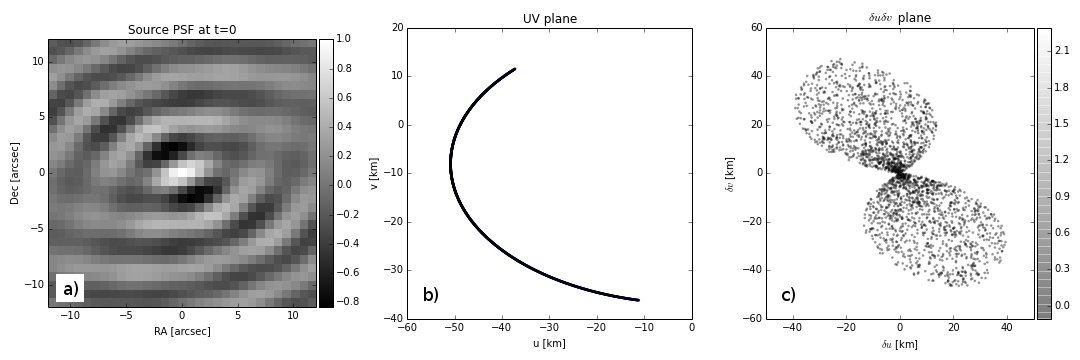
\includegraphics[width=\textwidth]{images/psfIM-dudv-labelled.png}
\caption{\label{plot.psf.uv.dudv} Fig. \ref{plot.psf.uv.dudv}a shows the PSF image of a simulated 1Jy source at phase centre. {Colourbar units are in Jansky}.  Fig. \ref{plot.psf.uv.dudv}b shows the associated UV track, and Fig. \ref{plot.psf.uv.dudv}c the corresponding $\left(\deltu,\deltv\right)$ tracks. Note that the $\deltu\deltv$ plane does not have a homogeneous point density, but is denser near its origin: here, this is shown by plotting only 1 random point in 10000.}
\end{figure*}


{Since the variance fluctuations act as tracers for calibration artefacts, artefacts in the image can be understood as \emph{one realisation} of the variance map, which is characterised by an average level determined by the variance in the gains and thermal noise, and a noise-PSF convolved with the sky brightness distribution}. The actual artefacts in the image will still be noisy, as a realisation of the true variance map. For the same reason, in the absence of correlated gain errors, $[\Cov{\matGains}]_{b \ne b'}$ are all zero and $\Cov{\matGains}$ is a diagonal matrix. {We then recover a ``flat" noise-map: the variance will be the same in all pixels, as the noise-PSF is absent}. In the ideal case, were we to recover the true value of the gains for all times and frequencies, this becomes pure thermal noise.
\subsection{Noise Map Simulations}\label{sec.simulations}



\begin{figure}[h!]
\centering
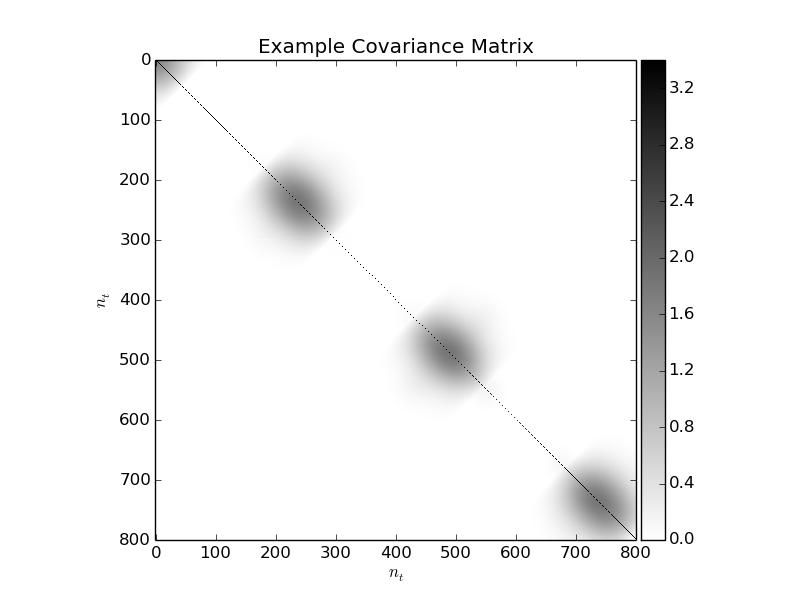
\includegraphics[width=0.8\textwidth]{images/CovarianceMatrix.png}
\caption{\label{fig.covmat} Example of {a non-stationary covariance matrix}, which can be used to simulate $\Cov{\matGains}$.{The colourbar units are Jy$^2$}. The correlation scale $\sigma_\tnuIndeix$ is 40 cells, and the variability period is 500 cells. The matrix is made positive semi-definite (and therefore a covariance matrix) through SVD decomposition. The maximum size of the ``bubbles" is determined by $\sigma_\tnuIndeix$.}
\end{figure}


\pg
We have shown in Eq. \ref{eq.covcov.matrix} that there exists an analytical relationship between residual visibility statistics and image-plane residual statistics. This section gives details of simulations we have performed to support our claims on this ``Cov-Cov" relationship. Specifically, we simulate residual visibilities for a single baseline by generating a set of correlated random numbers with zero mean and a distribution following a specified covariance matrix $\bm{C}$. 
It contains a periodic function of period $T$ along the diagonal, which is then convolved with a Gaussian of width $\sigma_\tnuIndeix$ corresponding to the characteristic scale of correlation. The values of these parameters are chosen arbitrarily. A small constant term is added on the diagonal, the net value of which is strictly positive. This simulates a low thermal noise. Finally, singular value decomposition is used to ensure that this matrix is Hermitian positive semi-definite. The net effect is a {non-stationary} correlation: some residuals are correlated with their neighbours, and uncorrelated with others. An example of this covariance matrix for arbitrary parameter values is shown in Fig. \ref{fig.covmat}. We see that, for any given point, correlation is stronger with some neighbours than others (as determined by $\sigma_\tnuIndeix$).
Samples are drawn as follows: $\bm{C}$ is built following user specifications as described above. We then find its matrix square root $\bm{C}_0$ so as to apply it to random numbers generated from a normal distribution. We generate 2000 realisations $i$ of our random variables $\bm{r}_i$: 
\begin{alignat}{2}
\muely_i &= \sum_b \muelF_b \bm{r}_i \quad &\mathrm{with} \quad \bm{r}_i =& \bm{C}_0 \bm{x}\\
         &                                 &\mathrm{and} \quad \bm{x} \leftarrow& \mathcal{N}\left(0,1\right)\\
\muely   &= \begin{pmatrix} \hdots \muely_i \hdots \end{pmatrix}
\end{alignat}
{where $\muely$ is a matrix of dimensions $n_{\mathrm{realis}}\times n_b$. Since $\bm{x}$ follows a normal distribution, $\Cov{x}=\I$ and the covariance matrix of each $\muely_i$ is, by construction, $\bm{C}=\bm{C}_0 \bm{C}_0^H$. The covariance matrix of $\muely$ is thus also $\bm{C}$.}


\pg
As for the $uv$-track, our simulations read a single one from a specified dataset. In this case, we read an 8-hour $uv$-track for a baseline between two arbitrary LOFAR stations (specifically, CS001HBA0 and RS310HBA) in an observation of the Bootes extragalactic field. The effective baseline length varies between 37.9km and 51.8km. The dataset included 20 channels, each with a spectral width of 97.7 kHz; the central observing frequency is 139 MHz. The temporal resolution is 1 measurement per second.

We compare the \emph{measured} variance map $\bm{V}_y^m$, built by measuring the variance across realisations at each pixel in the image-plane, with the \emph{predicted} variance map $\Var{\muely}$, built using the Cov-Cov relationship (Eq. \ref{eq.covcov.matrix}). Since we are only interested in the variance map, rather than the covariance between pixels, we compute only the diagonal terms.
\begin{alignat}{2}
\bm{V}_{\tilde{y}}^m &= \diag{\muely\muely^H} \label{eq.meas.var}\\
\bm{V}_{\tilde{y}}^{pr} &= \sum_b [\bm{C}] _{bb}\I + \sum_{b,b'\ne b}\diag{\muelF_{bb'}}[\bm{C}]_{bb'}\label{eq.theo.var}
\end{alignat}
where the thermal noise is already incorporated into the diagonal of $\bm{C}$ and Eq. \ref{eq.theo.var} is merely the diagonal operator applied to the Cov-Cov relationship. 



\begin{figure*}[h!]
\centering
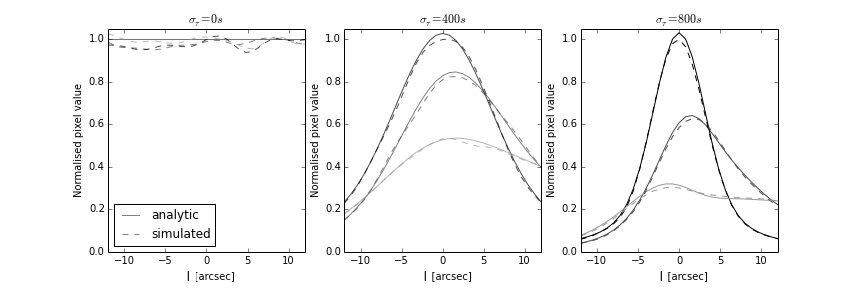
\includegraphics[width=\textwidth]{images/cross_sections1.png}
\caption{\label{plot.cross-sections} The three lines in each figure correspond to three horizontal cross-sections from images in Fig. \ref{plot.noisepsfs}. {The units on the y-axis are dimensionless [$Jy^2/Jy^2$].} $\sigma_\tnuIndeix$ is the maximum characteristic error correlation length. In decreasing intensity, they correspond to  $m=0''$, $m=4''$, and $m=8''$. The dashed lines correspond to the variance measured with 2000 realisations for each pixel, while the solid line corresponds to the predicted value at that pixel. There are 31 pixels. We do not show cross-sections for negative $m$ due to image symmetry about the origin.}
\end{figure*}



\subsubsection{Simulation with a single point source}

\pg
We model our sky as containing a single 1 Jy point source at phase centre: we thus have $\phi_{bb}=w_b^2$. The source as seen through the set of $uv$-tracks used in our simulation, along with their corresponding $\left(\deltu,\deltv\right)$ space, are shown in Fig. \ref{plot.psf.uv.dudv}. The \emph{simulated} noise-map is calculated by drawing a large sample ($n_\mathrm{realis}=2000$) of random numbers from the correlated distribution, thereby creating 2000 sets of residual visibilities. By Fourier-transforming the visibilities to the image-plane and taking the variance of the values for each image pixel (i.e. each $l,m$ pair) as per Eq. \ref{eq.meas.var}, we can estimate $\Var{\muely}$. The \emph{predicted} noise-map, meanwhile, was found by assigning each cell of $\bm{C}$ to the appropriate point in the $\left(\deltu,\deltv\right)$ plane and Fourier transforming from this plane into the image-plane, as per Eq. \ref{eq.theo.var}.
We compare the outcome of simulating a large number $n_\mathrm{realis}$ of realisations and taking the variance across these realisations for each pixel with mapping the covariance matrix onto the $\deltu\deltv$-plane and using the Cov-Cov relationship.The results of our simulations are shown side-by-side in Fig. \ref{plot.noisepsfs}: the predicted and simulated noise-PSFs match. The peak-normalised predicted noise-PSF is less noisy, as shown in Fig. \ref{plot.cross-sections} for different correlation scales. This is expected, since it is calculated directly from the underlying distribution, rather than an estimate thereof. As $n_\mathrm{realis}\rightarrow\infty$, we expect the two methods to fully converge. As the maximum characteristic correlation length $\sigma_\tnuIndeix$ increases, the variance becomes ever more sharply peaked.

\begin{figure}[h!]
\centering
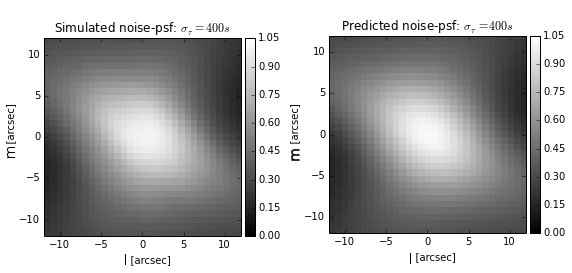
\includegraphics[width=\textwidth]{images/noisepsf-ctime400.png} %{../../../SkyCoverageMap.png} %
\caption{\label{plot.noisepsfs} Simulated noise-maps, compared with theoretical prediction. The pixel values are normalised by the average value of the covariance matrix: the units of the colourbar are thus dimensionless ($Jy^2/Jy^2$). These are on the same angular scale as the source shown in Fig. \ref{plot.psf.uv.dudv}.}
\end{figure}

\pg
{Since our simulated sky consists of a 1Jy source at phase centre, there is only one noise-PSF to modulate the average noise-map, and it lies at phase centre. Let us test our formalism further by considering a model with multiple point sources.}

\subsubsection{Simulation with 3 point sources}

\pg
{We wish to test our prediction that the noise-map can be described as a convolutional process modulating an average noise level. We thus perform another simulation, this time with three 1Jy point sources. The associated dirty image is shown in Fig. \ref{imag.simu-3sources.noisemap}d. }



\pg
{This dirty image simply consists of performing a direct Fourier transform (i.e. without using a Fast Fourier Transform algorithm) on simulated visibilities corresponding to these three point sources. We now perform a similar test as above on this field. Firstly, we ``apply" gain errors to these visibilities by multiplying our model with our residual gain errors. This allows us to find 2000 realisations of residual visibilities, and find the variance for each pixel across these realisations. This gives us the simulated noise-map, shown in Fig. \ref{imag.simu-3sources.noisemap}a. Secondly, we perform a DFT from the differential Fourier plane to the $(l,m)$ plane as before, assigning one cell of $\Cov{\matGains}$ to each point of the differential Fourier plane. This time, however, $\phi_{bb'}^d$ is not simply unity for all points in the differential Fourier plane. Instead, it is calculated for the three-point-source model, and applied for each point. This gives us the predicted noise-map in Fig. \ref{imag.simu-3sources.noisemap}b. Finally, Fig. \ref{imag.simu-3sources.noisemap}c shows the absolute value of the difference between the two images. We see that there is some structure present in these residuals: this is expected, as the PSF of the sources in the dirty imags clearly overlap. We are thus not quite in the regime where emission is from well-separated point sources. Nevertheless, our predictions hold to better than $5\%$ accuracy. }

\begin{figure}[h!]
\centering
\includegraphics[width=\textwidth]{images/Ctime6400-noisePSFandDirty-uncorr.png}
\caption{\label{imag.simu-3sources.noisemap} {Noise-map of sky with correlated gain errors and three point sources. The colourbars of (a), (b) and (c) have dimensionless units, while that of (d) is in Jansky. Note the presence of structure in the residuals (c): these show the limits of our hypothesis that sources are well-separated.}}
\end{figure}

\pg
It bears repeating that, for correlated noise, this map can be understood as a distribution map for calibration artefacts: the amount of spurious correlated emission seen by each baseline will determine the noise-map, and the true image-plane artefacts will then be \emph{one set of realisations} of this \emph{underlying distribution}.

\section{Adaptive Quality-based Weighting Schemes}\label{sec.DynamicRange}

\pg
As discussed in Section \ref{sec.intro}, some intervals of an observation will have lower gain variability. These will show up in the gain covariance matrix as intervals with lower variance. Similarly, those with larger intrinsic gain variability will have greater error in their gain estimate. By giving greater weights to the former, and lower weights to the latter, we expect to be able to improve image reconstruction. {We thus talk of adaptive quality-based weighting, as the weights will adapt based on the calibration quality.}

\pg
The pixel variance is determined by the visibility covariance matrix, as shown in Eq. \ref{eq.variance.imgplane}. The diagonal of the visibility covariance matrix will add a flat noise to all pixels, while its wings will determine the calibration artefact distribution, which will be convolved to the sky brightness distribution. We thus have two sources of variance in the image-plane.
Minimising the far-field noise (i.e. the variance far from sources) in an image would involve down-weighting noisier calibration intervals while up-weighting the more quiescent ones, without taking noise-correlation between visibilities into account. This is because the far-field noise will be dominated by the diagonal component of the covariance matrix (cf. Eq. \ref{eq.variance.imgplane}). By the same token, minimising calibration artefacts would involve down-weighting measurements with strongly-correlated noise, and up-weighting the less-correlated. This would not, however, minimise the diagonal component: in fact, it will likely exaggerate its up-weighting and down-weighting. As such, it will increase the constant level of the noise-map, but flatten the noise-PSF's contribution. There are thus two competing types of noise that we seek to minimise: uncorrelated noise, which corresponds to $\dudv=0$ (i.e. the diagonal components of the gain covariance matrix), and correlated noise, which corresponds to $\dudv\ne 0$ (i.e. its wings). Minimising the first will minimise far-field noise without optimally reducing artefacts, while minimising the last will minimise noise near sources at a cost to far-field noise. In the following sub-sections, we will discuss weighting schemes used to accomplish this.


\subsection{Optimising sensitivity}\label{sec.lightweights.formalism}


\pg
The Cov-Cov relationship (Eq. \ref{eq.covcov.matrix}) tells us that, far from any sources, the variance map (Eq. \ref{eq.variance.imgplane}) is dominated by a constant term: the contribution from thermal noise and the diagonal of the residual visibility covariance matrix. Maximising sensitivity far from sources therefore implies minimising $\diag{\Cov{\matGains}}$. This is equivalent to assigning visibilities weights inversely proportional to their variance:
\begin{align}
w_{b} &= \frac{1}{\Var{\matGains_{b}}}
\end{align}

\pg
For each baseline, those times with larger variance in the residuals will be down-weighted, and those with smaller variance will be up-weighted; this scheme does not require information about the underlying gains, only the error on our solutions. Since we are treating $\sigma_n^2$ as a constant for all antennas and all times, those times where our gains estimate is closer to the true gains will be up-weighted, and those moments where they are farther from the actual gains will be down-weighted: hence the term ``adaptive quality-based weighting". Note that the diagonal of the weighted residuals' covariance matrix should therefore become constant: this weighting scheme explicitly brings the residuals closer to what is expected in the case of perfect calibration, assuming uncorrelated noise. For the remainder of this paper, we will refer to these weights as \emph{sensitivity-optimal} weighting.



\subsection{Minimising Calibration Artefacts}\label{sec.fullweights.formalism}

\pg
Minimising calibration artefacts - i.e. optimising the sensitivity near bright sources - means flattening the noise-map. Since the noise-map can be understood as a noise-PSF convolved with all the modeled sources in the sky {modulating the background variance level,} it will be flattest when its peak is minimised. From the Cov-Cov relationship (Eq. \ref{eq.covcov.matrix}), we can see that, at the peak of the noise-PSF (which would be the variance at the pixel where $l=m=0$), the Fourier kernel is unity: the variance for that pixel is thus the sum of all the cells in the covariance matrix. By accounting for normalisation, we can write the variance at the centre of the noise-PSF as:
\begin{align}
V\left(\bm{w}\right) = \frac{\bm{w}^T {\Cov{\matGains}}\bm{w} }{\bm{w}^T \mathbf{1} \mathbf{1}^T \bm{w}}
\end{align}
Our optimality condition is then, after some algebra:
\begin{alignat}{2}
0 &=\frac{\partial}{\partial \bm{w}}\left( V \right)\\
\leftrightarrow
\Cov{\matGains} \bm{w} &= \mathbf{1}\mathbf{1}^T \bm{w} \left(\bm{w}^T \bm{1}\bm{1}^T\bm{w}\right)^{-1} \bm{w}^T\Cov{\matGains} \bm{w}
\end{alignat}


\pg
We find that one $\bm{w}$ which satisfies the above is:
\begin{align}
\bm{w} &= \Cov{\matGains}^{-1} \mathbf{1}\label{eq.fullweights.analytical}
\end{align}
where $\mathbf{1}$ is a vector of ones. Provided that the hypotheses made so far hold\footnote{Specifically, that the residual visibilities do not contain any true signal, i.e. that all sources have been properly subtracted from the visibilities}, these weights depend only on calibration quality: badly-calibrated cells will include spurious time-correlated signal introduced by trying to fit the noise $n$ on visibilities. Down-weighting these cells helps suppress artefacts in the field, at the cost of far-field sensitivity. This weighting scheme is thus only a function of the relative quality of calibration at different times, boosting better-calibrated visibilities and suppressing poorly-calibrated visibilities. For the remainder of this paper, we will refer to these weights as \emph{artefact-optimal} weighting.

\section{Estimating the Covariance Matrix}\label{section.algorithm}
\pg
In our simulations, we have worked from a known covariance matrix and shown that our predictions for the residual image's behaviour hold. With real data, however, we do not have access to this underlying covariance matrix. Since our weights are extracted from said matrix, estimating it as accurately as possible remains a challenge: this is in turn limited by the number of samples which can be used for each cell.

\pg
Each cell in the covariance matrix is built by averaging a number of measurements, or samples. The more samples are available, the better our estimate becomes: once we have more samples than degrees of freedom, we say that our estimation is well-conditioned. Otherwise, it is poorly-conditioned. In this section, we will discuss ways in which we can improve the conditioning of the covariance matrix estimation.

%
\subsection{Baseline-based Estimation}

\pg
One way to improve the conditioning of our covariance matrix estimation is to make the same hypothesis as the calibration algorithm: we can treat the underlying gains as constant within each calibration interval. Provided this interval is known, this allows us to find a single estimate for each interval block of the covariance matrix, turning a $n_b\times n_b$ matrix into a smaller $n_{\mathrm{intervals}}\times n_{\mathrm{intervals}}$ equivalent, where $n_{\mathrm{intervals}}$ is the number of solution intervals used for to find the gain solutions. We then improve our conditioning by a factor of $n_\mathrm{int}$, which is the number of samples in a calibration interval. The estimate $\widehat{\Cov{\matGains}}$of the covariance matrix $\Cov{\matGains}$ is built by applying the covariance operator:
\begin{align}
\widehat{\Cov{\matGains}} \bydefn \estC =&  \frac{1}{n_\mathrm{int}}\sum_{i\in n_{\mathrm{int}}}\left(\matGains_i- \langle \matGains \rangle\right) \left(\matGains_i - \langle \matGains \rangle \right)^H
\end{align}
where the $\langle \hdots\rangle$ operator denotes taking the average over the full vector. If the calibration solver's gain estimates are unbiased (i.e. $\Exp{\ghatvect}=\gvect$) \emph{and} the model of the sky is sufficiently complete, this quantity should be zero. Having created $\estC$, which will be of size $n_b \times n_b$, its cells can now be averaged over blocks of $n_\mathrm{int}\times n_\mathrm{int}$. This allows us to estimate the weights for each baseline and each time.

\pg
Mathematically, we retrace the steps of Section \ref{sec.formalism}. In the absence of direction-dependent effects, we define the residual visibilities as before, and use them to define the normalised residual visibilities $\rho_b$:
\begin{align}
r_{b} =& w_b \kappa_b \tilde{\gamma}_b  + \epsilon \label{eq.residual.matrix}\\
\rho_{b} =& \frac{r_{b}}{k_b}
\end{align}
We then organise the residuals in cells:
\begin{align}
\Rmat{\cellindex} =&   \begin{pmatrix} \vdots \\ \rho_{b\in \cellindex} \\ \vdots \end{pmatrix}\\ % \bydefn \vecw_{\cellindex}\kvect{\cellindex}\matGains_{\cellindex} + \bm{n} \\
\bm{R} =&   \begin{pmatrix} \hdots \quad \Rmat{\cellindex} \quad \hdots \end{pmatrix}
\end{align}

\pg
$\bm{R}$ corresponds to a matrix containing all the residual visibilities within one calibration cell $\cellindex$, i.e. for $b \in \cellindex$ where $\gvect_{\cellindex} = \const$ {It is therefore of size $n_{\mathrm{intervals}}\times n_{\cellindex}$, where $n_{\mathrm{intervals}}$ is the number of calibration intervals in the observation}. Normalising the residual visibilities by $k_b$ allows us to recover the underlying covariance matrix by multiplying the residual visibility matrix $\bm{R}$ with its Hermitian conjugate:
\begin{align}
\estC[b\in\cellindex,b'\in\cellindex']             =& \left(\bm{R}^H \bm{R}\right)[\cellindex,\cellindex']
\end{align}
Note that we have divided the noise term by the flux model $S_b$, which can be very small in some cells. As such, care must be taken not to cause the relative thermal noise contribution to explode: those cells where this would occur are dominated by thermal noise, and information on the covariance matrix cannot be recovered from them.

\pg
In this framework, we simply treat the index $\cellindex$ as containing all the times and frequencies, for individual baselines, corresponding to a single calibration interval. $\estC$ is then an estimate of the residual visibility covariance matrix.



\subsection{Antenna-based Estimation}

In the subsection above, we assume{d} that finding one solution per interval will give us strong enough constraints to make the problem {of estimating the covariance matrix} well-conditioned: this may not be true in all cases. Conditioning may then need to be improved further: in this subsection, we show one way in which this can be done. There are others, e.g. using the rank of the matrix itself to find better-conditioned estimates of the covariance matrix at a lower resolution (i.e. a single estimate for a greater number of cells). They will not be presented in this paper, but are a possible avenue future work on this topic.

\pg
In estimating the covariance matrix for each baseline and each calibration cell, we are severely limited by the small number of samples in each cell. One way to overcome this problem is to find estimates for the variance of \emph{antenna} gains, and use these to return to the baseline variances. In this formalism, we extend  $\cellindex$ to include all visibilities pointing at a single antenna at a given time. Let us begin by writing an expression for the gain vector, which contains the gains for all antennas and all calibration cells:
\begin{align}
\ghatvect_c =& \begin{pmatrix} \vdots \\ \hat{g}_p^{\tnuIndeix\in c} \\ \vdots \end{pmatrix}\\
\Ghatvect =& \begin{pmatrix} \hdots \quad \ghatvect_c \quad \hdots \end{pmatrix}
\end{align}
and the variance on each antenna in each calibration cell is then:
\begin{align}
               =& \Exp{\ghatvect_c \ghatvect_c^H} - \underbrace{\Exp{\ghatvect_c} \Exp{\ghatvect_c}^H}_{= \gvect_c \gvect_c^H} \label{eq.def.vector.variance}
\end{align}

\pg
As we can see, Eq. \ref{eq.def.vector.variance} is simply a vector form of Eq. \ref{eq.residuals.definition}.
The residual gains of Eq. \ref{eq.residuals.definition} can now be understood as random samples of the covariance between the gains for antennas $p$ and $q$ at a given time, assuming complete skymodel subtraction. We can thus define the variance sample matrix as an \emph{estimate} of the \emph{variance matrix}:
\begin{align}
\VarmatC =&\widehat{\Var{\gvect_c}} \\
                   =& \sum_{\tnuIndeix\in\cellindex} \left( \ghatvect_\tnuIndeix\ghatvect_\tnuIndeix^H - \gvect_\tnuIndeix\gvect_\tnuIndeix^H \right)
\end{align}


\pg
We define the residual matrix as:
\begin{align}
\Rmat{\tnuIndeix} =& \sum_d s_d \Kmat{d,\tnuIndeix} \left( \ghatvect_\tnuIndeix\ghatvect_\tnuIndeix^H - \gvect_\tnuIndeix\gvect_\tnuIndeix^H \right) \Kmat{d,\tnuIndeix}^H + \epsilon \label{eq.residual.matrixform}
\end{align}
where we {explicitly place ourselves in the limits of our formalism, i.e.} that we do not have direction-dependent gains. We now see that at the core of Eq. \ref{eq.residual.matrixform} lies $\displaystyle\VarmatTau$, where $\sum_{\tnuIndeix\in\cellindex} \VarmatTau = \VarmatC$.
The K-matrix is defined as follows:
\begin{align}\label{kmat.def}
\Kmat{d,\tnuIndeix} =&
\begin{pmatrix}
k_{p,\tnuIndeix}^{d}   &                       &   0     &\\
                       & k_{q,\tnuIndeix}^{d}  &        &\\ 
         0              &                       & \ddots 
\end{pmatrix}
\end{align}
Since the residual matrix depends on the gains, we define the residual visibility vectors as:
\begin{align}
\Rmat{{\cellindex}} =&   \begin{pmatrix} \vdots \\ \Rmat{\tnuIndeix\in \cellindex} \\ \vdots \end{pmatrix} \\
\bm{R} =&   \begin{pmatrix} \hdots \quad \Rmat{c} \quad \hdots \end{pmatrix}
\end{align}

\pg
$\Rmat{\cellindex}$ corresponds to a matrix containing all the residual visibilities within one calibration cell $\cellindex$, i.e. for $\tnuIndeix \in \cellindex$ where $\gvect_{\cellindex} = \const$ Let us define $n_\cellindex$ as the number of elements in each calibration cell. The residual variance sample matrix can now be built by multiplying the residual visibility matrix with its Hermitian conjugate:
\begin{align}
\matVV             =& \bm{R}^H \bm{R} \label{eq.matvv.definition} %\\
\end{align}
Note that we do this because it allows us to turn a single noise realisation $\epsilon$ into a statistical quantity $\sigma$.
We can relate $\matVV$ to the variance of individual antenna gains:
\begin{align}
\matVV
            =& \sum_{\tnuIndeix\in\cellindex} \left(\sum_{d,d'} s_d \Kmat{d,\tnuIndeix} \left( \VarmatC \right)^H \Kmat{d,\tnuIndeix}^H s_{d'} \Kmat{d',\tnuIndeix} \left( \VarmatC \right) \Kmat{d',\tnuIndeix}^H + \I\sigma^2 \right)
\end{align}
To reach this point, in Eq. \ref{whocares}, we made the hypothesis that the sky brightness distribution is dominated by emission from well-separated point sources. Applying this hypothesis again here, we can make the approximation that the cross-terms in the sum over $d,d'$ average to zero: $\sum_{d,d'\ne d}\approx 0$. We then have:
\begin{align}
\matVV\approx& \sum_\tnuIndeix \left(\sum_d s_d^2 \Kmat{d,\tnuIndeix} \left( \VarmatC \right)^H  \left( \VarmatC \right) \Kmat{d,\tnuIndeix}^H + \I\sigma^2\right)\\
            =& \left(\VarmatC\right)^2\hadam \left(\underbrace{\sum_{\tnuIndeix}\sum_d s_d^2 \kvect{d,\tnuIndeix}\kvect{d,\tnuIndeix}^H}_{\bydefn \mathcal{S}}\right) + n_\cellindex\I\sigma^2\\
\VarmatC    =& \sqrt{\mathcal{S}^{\hadam-1}\left(\matVV-n_\cellindex\I\sigma^2\right)}
\end{align}
where $\hadam$ denotes the Hadamard or entrywise product and $\kvect{}=\diag{\Kmat{}}$. % If $\matVV$ is diagonal, the gains are uncorrelated and the above can be written as:
Thus, $\matVV$ allows us to estimate the variance of each antenna and for each calibration cell by using all the visibilities pointing to that antenna within that calibration cell. With this information, we can then rebuild the baseline-dependent matrix, having improved our sampling by a factor of $n_{\mathrm{ant}}$.


\section{Applying the Correction to Simulated Data}\label{section.simulations.application}


\pg
In this section, we show the impact of our weighting schemes on a noise-map made from arbitrarily strongly-correlated residuals. Here, we assume that our sky contains only a single point source at phase centre: there is thus only a single instance of the noise-PSF, placed at phase centre, to modulate the average variance level. We sample this instance by taking a cross-section from $\left(l,m\right)=0$ to a large $l$, keeping $m$ constant. The only difference between these cross-sections is the weighting scheme applied: unit weights for all visibilities (``Uncorrected", blue), sensitivity-optimal weights (green), and artefact-optimal weights (red). We plot both the result predicted by the Cov-Cov relationship (solid line) and the variance estimated across 2000 realisations (dashed line): the result is shown in Fig. \ref{fig.simu.weightapplied}. The two remain in such agreement throughout the cross-section as to be nearly indistinguishable. 



\begin{figure}[h!]
    \centering
        \centering
        \includegraphics[width=\linewidth]{images/ctime001-NoisePsfCrossections-backup.png} 
        \caption{The sensitivity-optimal (green) and artefact-optimal (red) weights both give improvements over the unweighted noise-map (blue).} \label{fig.simu.weightapplied}
\end{figure}

\pg
There are a few significant points to note on this figure. Firstly, most of the power in the matrix lies along the diagonal: both weighting schemes thus give good improvements in variance across the map. The artefact-optimal weights, while decreasing the peak further, as expected, also increases the noise far from sources: this is due to the fact that the artefact-optimal weights are in a sense more ``selective" than the sensitivity-optimal weights: they up-weigh and down-weigh more severely, and will only result in a constant covariance matrix if this matrix is zero everywhere outside of the diagonal. {In effect, the noise-map becomes flatter, but much broader.}

\section{Applying the Correction to Real Data}





\pg
In this section, we show the effect of adaptive quality-based weighting on real data. The dataset used in this section is a single sub-band from an 8-hour LOFAR observation centred on the Extended Groth Strip ($\alpha$=14:19:17.84,$\delta$=52:49:26.49). The observation was performed on August 28th, 2014. The subband includes 8 channels of width 24.414 kHz each, for a total bandwidth ranging from 150.2 to 150.4 MHz. The data have been averaged in time to 1 data point per second. The data was calibrated using Wirtinger calibration \citep[see][and references therein]{2014arXiv1410.8706T,2015MNRAS.449.2668S} and a sky model consisting only of a nearby calibrator source, 3C295. A reference image (a cutout of which is shown in Fig. \ref{image.3c295.goodcal}) was made by calibrating the data according to best practice for LOFAR survey data: 1 calibration solution per 8 seconds and per 4 channels. {The residual data was then corrected by the gain solutions and imaged} using Briggs weighting (robust=0), pixel size of $1.5''$, and deconvolved using the default devoncolution algorithm in DDFacet \citepads{2017arXiv171202078T}.

\pg
The data was then time-averaged to create a new, 2.4 GB dataset with 1 data point per 8 seconds. Deliberately poor calibration was then performed on this dataset, solving for 1 calibration solution per 2 minutes ({\it caeteris paribus}). The resulting corrected residual data was imaged using the same imaging parameters as the reference image, and a cutout of the result is shown in Fig. \ref{image.3c295.nocorr}. As expected, the very long calibration intervals introduce calibration artefacts in the image. The brightest sources are still visible, but much of the fainter emission is buried under these artefacts. We are then in a case where our residual visibilities are dominated by calibration error rather than sky model incompleteness.

\pg
Weights were then calculated based on the badly-calibrated residual visibilities. Fig. \ref{image.3c295.lightcorr} was made using the same visibilities as Fig. \ref{image.3c295.nocorr} and applying baseline-based, sensitivity-optimal weight. Similarly, Fig. \ref{image.3c295.fullcorr} used the poorly-calibrated residual visibilities with the application of baseline-based, artefact-optimal weighting. These weights are likely to be poorly-conditioned. In both cases, all other parameters were conserved.

\begin{figure}[h!]
\centering
\begin{subfigure}{.49\textwidth}
\resizebox{\hsize}{!}{\includegraphics{images/paperfig-goodcal.png}}
\caption{\label{image.3c295.goodcal} Well-calibrated, unweighted restored image of the sky near the centre of the Extended Groth Strip. Used for comparison with the other images. {Units of colourbar are Janskys}. This image was made with data calibrated following best practice (solution intervals of 8 seconds, half the bandwidth). rms=5.87mJy/beam}
\end{subfigure}
\hfill
\begin{subfigure}{.49\textwidth}
\resizebox{\hsize}{!}{\includegraphics{images/paperfig-noweights.png}}
\caption{\label{image.3c295.nocorr} Poorly-calibrated, unweighted restored image of the sky near the centre of the Extended Groth Strip. {Units of colourbar are Janskys}. This image was made with the same data as for Fig. \ref{image.3c295.goodcal}, but averaged in time and calibrated using larger gain solution intervals: 2 minutes and half the bandwidth. rms=86.4mJy/beam}
\end{subfigure}
\hfill
\begin{subfigure}{.49\textwidth}
\resizebox{\hsize}{!}{\includegraphics{images/paperfig-cyrilweights.png}}
\caption{\label{image.3c295.lightcorr} Image made using the same imaging parameters and corrected visibilities as Fig. \ref{image.3c295.nocorr}, using sensitivity-optimal weighting. {Units of colourbar are Janskys}. rms=9.69mJy/beam}
\end{subfigure}
\hfill
\begin{subfigure}{.49\textwidth}
\resizebox{\hsize}{!}{\includegraphics{images/paperfig-fullweights.png}}
\caption{\label{image.3c295.fullcorr} Image made using the same imaging parameters and corrected visibilities as Fig. \ref{image.3c295.nocorr}, using artefact-optimal weighting. {Units of colourbar are Janskys}. rms=15.8mJy/beam}
\end{subfigure}
\caption{\label{image.fourRealImages}Restored images of the centre of the Extended Groth Strip, as seen with an 8-hour observation using the full LOFAR array. Fig. \ref{image.3c295.goodcal} shows an image of the field made with good calibration intervals. Fig. \ref{image.3c295.nocorr} shows an image of the field made with poor calibration intervals. Fig. \ref{image.3c295.lightcorr} shows image made with the same visibilities and imaging parameters, but with the application of the sensitivity-optimal weighting scheme. Fig. \ref{image.3c295.fullcorr}, similarly, differs from Fig \ref{image.3c295.lightcorr} only in that artefact-optimal weights, rather than sensitivity-optimal weights, were used. {The histograms of pixel values in each image have 1000 flux bins ranging from -0.16 Jy to 0.16 Jy. Their ordinates are in log scale.} Pixel size is 1.5'' in all images.}
\end{figure}

\pg
Note that applying antenna-based sensitivity-optimal weighting to the badly-calibrated data (not shown here) allows us to recover the reference image with only a very small increase in rms (increased by a factor of 1.14). Further testing on complex field simulations will be required to ascertain the usefulness of artefact-optimal weighting: it is likely that it fails to correct the image fully due to the poor conditioning of the covariance matrix used here.

\begin{figure}[h!]
\begin{subfigure}{.49\textwidth}
\resizebox{\hsize}{!}{\includegraphics{images/paperfig-goodcal.png}}
\caption{\label{image.3c295.goodcal-2} Well-calibrated, unweighted restored image of the sky near the centre of the Extended Groth Strip. Used for comparison with the other images. Calibration solution intervals used were 8 seconds, half the bandwidth. rms=5.87mJy/beam}
\end{subfigure}
\hfill
\begin{subfigure}{.49\textwidth}
\resizebox{\hsize}{!}{\includegraphics{images/paperfig-antweights.png}}
\caption{\label{image.3c295.antcorr} Image made using the same imaging parameters and corrected visibilities as Fig. \ref{image.3c295.nocorr}, with the application of antenna-based, sensitivity-optimal weighting. Solution interval of 2 minutes, half the bandwidth. rms=6.69mJy/beam}
\end{subfigure}
\caption{\label{image.twoRealImages}Comparison between the well-calibrated image (i.e. the same image as Fig \ref*{image.3c295.goodcal}) and antenna-based sensitivity-optimal weights.  {Units of both colourbars are Jansky}. We see that we recover a very similar image, despite the fact that the data used for the weighted image are averaged by a factor of 8 compared to those used for the unweighted image.}
\end{figure}

\pg
{The pixel histograms show us that the weights do not completely mitigate the poor calibration interval choice, but certainly give a dramatic improvement over the unweighted, poorly-calibrated residuals. This is compatible with our statement that the weights give similar residuals in the image with a dramatic improvement in time at some cost in sensitivity. It is interesting to note that while Fig. \ref{image.3c295.fullcorr} looks noisier than Fig \ref{image.3c295.lightcorr}, its residual flux histogram is actually closer to that of Fig. \ref{image.3c295.goodcal}.}

\pg
As for performance, the weights used for Fig. \ref*{image.3c295.fullcorr} took 8 hours of computing time on a single core\footnote{Core type: Intel(R) Xeon(R) CPU E5-2660 0 @ 2.20GHz}, working on a 29 GB dataset, which is not particularly large for LOFAR data. Since the problem is massively parallel, this cost can be alleviated. The main bottleneck is likely due to very poor code optimization. As for the weights used for Fig. \ref*{image.3c295.antcorr}, they are computed in 1min 6s on the same single core. 


\section{Discussion}

This chapter began by investigating the use of an algorithm inspired by ``lucky imaging'' to improve images made using radio interferometric data. By investigating the statistics of residual visibilities, we have made the following findings:

\begin{itemize}
\item A relationship between the statistics of residual visibilities and residual pixel values (the ``Cov-Cov relationship'').
\item A description of the noise-map in the image plane {as a constant variance level modulated by a noise-PSF convolved with the sources in the field. This gives }the variance in the flux of the image as a function of distance from the sources in the sky for a given calibration.
\item {An Adaptive Quality-Based weighting scheme, which reduces the noise in the image (and the presence of calibration artefacts) by minimising either the constant noise term or the noise-PSF.} 
\end{itemize}

\pg
%In effect, we have provided a basis to justify the use of unpublished, but still commonly-used, methods like ``clipping'' statistically outlying calibration gains. 
{While our results are not a panacea for poor calibration, they show that we can not only improve images made with well-calibrated data, but also mitigate the worst effects of poorly-calibrated visibilities in otherwise well-calibrated datasets. Provided that the gain variability timescale is long enough at certain points of the observation, we can effectively get images of similar quality using both the} ``standard'' best-practice calibration interval for LOFAR survey data (calibration solution interval of 8 seconds) and a significantly larger solution interval of 2 minutes (frequency interval unchanged). {Of course, if no such stable interval exists, there will be no good intervals to upweigh, and we will be left only with equally-poor data chunks.} This means that{, in the right conditions,} net pipeline time {can be} sped up by a factor of nearly three, at a slight cost in sensitivity. {This increase will be greater than what could be achieved with existing comparable methods such as ``clipping''.} However, it does not aim to replace such methods, but rather to act as a complement to them: clipping will be better at flagging a handful of bad visibilities, while this weighting scheme will help push the general visibility statistics (and therefore the image-plane statistics) towards a better distribution.

\pg
We emphasize that the adaptive quality-based weighting schemes work because the noise-{map} describes the \emph{underlying noise distribution}, of which calibration artefacts are \emph{one single realisation}. To fully characterise the artefacts, the correlation between different pixels (i.e. off-diagonal elements of $\Cov{\muely}$) must be computed; this has not been done in this paper. Nevertheless, lesser constraints on the spatial distribution of artefacts can be found using only the diagonal elements of $\Cov{\muely}$. The weighting schemes merely seek to {minimise} this spatial distribution as much as possible: the end result is \emph{fewer artefacts}, {which can be} distributed across a \emph{much larger area}. {This} is the source of the dramatic improvement from \ref{image.3c295.nocorr} to Fig. \ref{image.3c295.lightcorr}. We have simply down-weighted those visibilities where spurious signal was introduced by the calibration solutions, and up-weighted those visibilities where such signal was lesser. Since this spurious signal is the source of calibration artefacts, downweighting the associated visibilities reduces it dramatically. {The poor improvement from Fig. \ref{image.3c295.nocorr} to \ref{image.3c295.fullcorr}  is likely due to limits in the conditioning of our estimation of the covariance matrix.}

\pg
The work presented here can be improved upon, notably by working on improving the conditioning of our covariance matrix estimate: {for real observations}, it is impossible to have more than one realization of each gain value for all antennas. By treating each visibility within a calibration {interval} as a realization of the true distribution, we can better estimate the covariance matrix per baseline, and thus reach a better estimate of the variance in the image-plane. Of course, in practice, we can never access to the true, underlying time-covariance matrix for each baseline. Significant hurdles remain:
\begin{itemize}
\item The impact of sky model incompleteness (since calibration requires a sky model) is ignored in this paper; we start by assuming that we have a complete sky model. In practice, of course, acquiring a complete sky model is often a key science goal in and of itself. The impact of this hypothesis therefore ought to be investigated in future work.
\item The conditioning of our covariance matrix estimation remains a concern. By using an antenna-based approach, we can improve conditioning by a factor of $n_{ant}$, but this is only one approach among many. Further work is needed to investigate which method, if any, proves optimal.
\end{itemize}
%
%%
%%% % % Chapter 5 - strategy
%%\cleardoublepage
%%\chapter{Scientific Overview: Goals \& Strategy}
\minitoc
%\pg
%This section aims to provide a general overview of our scientific aims \& chosen strategy. [describe more]

\section{Science Goal}
\pg
So far, we have shown the technical work done on interferometric techniques as part of this PhD. In this section, we outline the application of this work, along with other modern tools, to the creation of large, deep and high-resolution surveys of the sky. While this approach is potentially extremely rewarding in terms of the science one can do with its resulting maps, it is also uniquely complicated.

\pg
Why, then, use this approach? One reason is the challenge itself. A high-resolution (matching HST resolution), wide-area (multiple degrees wide), high-quality\footnote{Reliably artefact-free, with known \& limited decorrelation, etc.} radio survey has \emph{never} been achieved at the time of writing. Many surveys of the radio sky exist, of course, but they tend to combine only two of those three qualities. FIRST \citepads[see][and references therein]{2015ApJ...801...26H}, for example, has achieved tremendous results with a $4''$ resolution, relatively low sensitivity, and no short baselines (thereby missing diffuse emission and extended structure) at $\sim$1.4 GHz. The VLASS \citepads[see][and references therein]{2013arXiv1312.4602H} will aim to go to a $2.5''$ resolution, medium sensitivity, and few short baselines - at frequencies ranging from 2 to 4 GHz. There exist many LOFAR HBA ($\sim$120-240 MHz) sky surveys \citepads[cf.]{2016MNRAS.460.2385W,2017A&A...598A.104S}, but they do not yet make use of international LOFAR, and are thus limited in resolution ($\sim 5''$).%Finally, there will of course be the SKA1-MID survey once the SKA is operational; this survey is expected to provide excellent resolution, sensitivity, and good $uv$-coverage, making it sensitive to diffuse emission as well as point sources.

\pg
In this context, a sky survey made using international LOFAR would be competitive until the SKA-MID survey (and considering it maps the Northern sky rather than the Southern sky, would arguably remain competitive even then). It would also allow LOFAR to fulfill the role of pathfinder in a very literal way, by providing datasets on which algorithms and imaging strategies could be tested before handling SKA data volumes in real-time.

\pg
Making a high-resolution full-sky survey using international LOFAR is thus arguably useful in and of itself in terms of interferometric techniques \& instrumentation. What then of its science value? The two most obvious advantages of a good large-sky survey are that they are complete (i.e. they are an accurate sample of the underlying source distribution, up to the survey's limiting flux)  while still giving information on rare outlier objects which may happen to lie in the field. This gives us access to a wealth of statistics from which to derive more robust estimations of population distributions. %Furthermore, depending on the quality of a given survey, it might even be able to provide such statistics simultaneously for various different fields of scientific interest.

\pg
Of course, LOFAR is already providing such catalogues - LOTSS \citepads[see][and references therein]{2017A&A...598A.104S}  is only the first of many to come. But these catalogues do not make use of the LOFAR international stations, and thus do not make full use of LOFAR's resolution ($5''$ resolution vs. $0.5''$).  This is so due to the technical challenges introduced by the use of international stations, which are due to decorrelation and an already limited signal-to-noise on those very short spatial frequencies.

\pg
What would they add to a LOFAR catalogue? A high-resolution sky survey has all the advantages listed above with more besides. For AGN science, for example, the higher resolution gives information on smaller scales, which is very relevant to study the turbulent processes in the lobes and the nearby intergalactic medium. We also know that there exist small AGNs: size therefore matters, and resolving these small AGNs (which tend to lie at larger redshifts, hence their smaller angular size) can give extremely salient information on AGN population distributions as a function of the age of the universe. Indeed, for AGN science, the LOFAR international baselines can be the difference between having absolutely no information on size distribution (no resolved AGN) and knowing everything about the AGN size distribution within a given extragalactic field. Finally, resolving sources is very relevant to spectral studies of AGN populations: we know very little about the physics of AGNs at low frequencies. Information on large populations of resolved sources (allowing us to separate compact structure from extended emission) is a prerequisite to begin the statistical work needed to understand these low-frequency AGN physics. As such, the international baselines can bridge a critical gap in the data available to peers studying AGN science.

\pg
AGN science is far from the only field which could benefit from the sub-arcsecond resolution that international LOFAR could provide. High-resolution imaging can be of tremendous interest to the study of star-forming galaxies: it could give insight into cosmic ray structure and access to spectral information. This is relevant because the entire star-forming history of galaxies is encoded in radio emission, but can only be accessed with sufficient spectral information and spatial resolution. A high-resolution survey, in particular, allows comparisons between optical and radio emission for known star-forming galaxies on a truly industrial scale, which would allow for the mapping of free-free absorption, supernova remnants, HII regions, etc...onto optical maps, and this for sources going up to high redshifts.

\pg
Of course, this does not run the full range of science cases which would benefit from high-resolution maps of large parts of the radio sky. Colleagues studying gravitational lensing would benefit greatly from large samples of lensed galaxies. Resolved extragalactic recombination lines (for bright objects) would doubtlessly interest peers studying galactic evolution. We expect these samples to be a natural byproduct of a large, high-resolution map of the radio sky: if they do not appear, that could indeed be a very interesting scientific result in and of itself.

\pg
More generally, high-resolution surveys provide high-resolution images of everyone's favourite objects and sources. It allows for better optical matching and identification, which is particularly relevant e.g. when needing to associate either a low-z or high-z sources to optical counterpart sources (in the case of the Extended Groth Strip, for example, using the international stations means matching the Hubble Space Telescope's resolution). They are thus a strong contribution to multi-wavelength datasets. It also improves the image's sensitivity to compact sources embedded in diffuse emission: if the source is better-resolved, then the emission associated with compact sources is more easily separated from emission emitted by its surroundings. This can be of tremendous help in image interpretation. Finally, actually resolving objects allows us to have better morphological classification for compact objects, which can be extremely useful e.g. when interested in AGN populations vs star-forming galaxy populations.




\section{3C295 and the Extended Groth Strip}

\pg
In this section, we briefly describe previous observations of the Extended Groth Strip (EGS), an extragalactic field with a rich multi-wavelength coverage described in Table \ref{table.EGS.observation}. It has been long observed as part of the All-Wavelength Extended Groth Strip International Survey collaboration (AEGIS, \citetads{2007ApJ...660L...1D}), which later became part of the CANDELS collaboration (\citetads{2011ApJS..197...35G}). The field is centred at $\alpha=14^h17^m,\delta=+52\deg 30'$, placing it between the tail of Ursa Major and Draco. Its size is $0.7'\times 0.1'$. It has notably been the subject of very deep Hubble Space Telescope observations, which the international LOFAR could attempt to match. 

\begin{table}[h!]
\begin{tabular}{cccc}
Telescope    & Band    & Resolution  & Area \\\hline
Chandra      & X-ray   & $0.5''-6.0''$ & $17'\times 120'$ \\
GALEX        & UV      & $5.5''      $ & 1.25$^\text{o}$ diameter \\
HST/ACS      & Optical & $0.1''      $ & $10' \times 67'$\\
HST/NICMOS   & Optical & $0.35''     $ & 0.0128 deg$^2$\\
Megacam      & Optical & $1.0''      $ & 1 deg$^2$\\
IRAC         & IR      & $2.0''      $ & $10' \times 120'$ \\
Spitzer      & IR      & $5.9''-19'' $ & $10'\times 90'$\\
VLA          & Radio   & $1.2''-4.2''$ & $30' \times 80'$
\end{tabular}
\caption{\label{table.EGS.observation}Table recapitulating the multi-wavelength coverage of the Extended Groth Strip, with observations performed as part of the AEGIS (later, CANDELS) collaborations.}
\end{table}

\pg
3C295 is a 3C\footnote{Third Cambridge Catalogue of Radio Sources, a 1959 survey of of the Northern radio sky} source, and thus one of the brighter sources in the Northern radio sky. It lies less than a degree away from the centre of the Extended Groth Strip, which has two important consequences: first, that it can potentially be used as a calibrator source for LOFAR; second, that unless well-modeled and subtracted at the observing instrument's maximum resolution, its sidelobes will pollute the EGS such that very little scientifically useful information might be recovered from a given observation.

\pg
The first step towards acquiring a deep, high-resolution image of the Extended Groth Strip therefore consists of creating a good, high-resolution model of 3C295 at LOFAR frequencies. Creating this model is one of the key results of this thesis. Starting from a high-resolution VLA model of 3C295, subbands selected across the LOFAR bandwidth are self-calibrated in iteratively greater numbers until a given noise threshold is reached. The flux scale is then boot-strapped based on the results of \citet{arse}. This ensures that 3C295 will be adequately subtracted from all corrected visibilities - including international baselines - and thus that images made using these visibilities will not be polluted by sidelobes from 3C295. 
The work done towards this goal is shown in \cref{section.3c295}. %, and its result - a high-resolution spectral model of 3C295 - is shown below.
%
%\pg
%\textcolor{red}{show key result here}

\section{Imaging the Full Primary Beam}
\pg
After creating a high-resolution model of 3C295 to calibrate the international stations, we must create a low-resolution model of all the sources in the primary beam to both improve final calibration quality and subtract sources outside of the Extended Groth Strip when creating the final high-resolution images.

\pg
Initial direction-independent calibration is done using the same pipeline as for the Lofar Two-metre Sky Survey \citepads[LOTSS,][]{2017A&A...598A.104S}. The killMS-DDF facet-based pipeline \citepads[cf]{2015MNRAS.449.2668S,2016ApJS..223....2V,2017arXiv171202078T} is then used to perform direction-dependent calibration for the entire LOFAR primary beam. This allows us to reach a noise threshold of $\sim$233$\mu$Jy.

\begin{figure}[h!]
\centering
\includegraphics[width=0.95\textwidth]{images/{lofar.widefield}.png}
\caption{\label{plot.EGS.lofar.widefield} Full direction-dependent calibrated image of the LOFAR primary beam, centred on the EGS. Image made without international stations.}
\end{figure}

\pg
This work, and its results, are shown in \cref{section.EGS.lowres}. Note that the AEGIS observations summarised in \cref{table.EGS.observation} do not cover the full LOFAR primary beam. The sources observed at low resolution are therefore matched with Sloan Digital Sky Survey (SDSS, \citetads{2000AJ....120.1579Y}) images. Overlays are shown to highlight the wealth of interesting sources, and their optical counterparts, which can be picked up as a byproduct of producing high-resolution maps of the radio sky. We select 12 particularly interesting sources and show the results of source matching for these candidates. Overlays of the same SDSS images with NVSS (NRAO VLA Sky Survey, \citetads{1998AJ....115.1693C}) postage stamps are also shown for comparison. Many of the chosen sources do not lie within the Extended Groth Strip, and are therefore only imaged at low resolution, but follow-up images and observations could be made should the need arise.

\section{Test Decorrelation}
\pg
Before launching the EGS imaging run using all calibrated datasets, we measure the impact of direction-dependent effects on known sources in the field. Two direction-dependent effects are expected to dominate: decorrelation and differential gains. The first is modeled by the imager used, whereas the second is a function of the gain variability as a function of distance from the calibrator. Seven calibrator sources, lying at various distances and directions from the calibrator source, are examined. They are summarised in \cref{table.LOBOS.sources}, which is reproduced below.

\begin{table}[h!]
\begin{tabular}{ccccc}
\# & RA [hms]    & Dec [dms]   & Dist. from EGS [deg.] & Dist. from 3C295 [deg.] \\\hline
1  & 14:30:18.72 & 52:17:29.80 & 2.041                         & 2.904 \\
2  & 14:19:44.44 & 54:23:04.58 & 1.928                         & 2.517 \\ 
3  & 14:21:20.05 & 53:03:46.00 & 0.864                         & 1.743 \\
4  & 14:21:09.41 & 51:22:32.46 & 1.294                         & 1.728 \\
5  & 14:11:50.32 & 52:49:02.66 & 0.844                         & 0.619 \\
6  & 14:11:20.23 & 52:12:04.30 & 0.915                         & 0.000 \\
7  & 14:08:07.00 & 52:55:11.36 & 1.409                         & 0.869 \\
8  & 14:08:09.76 & 52:44:46.56 & 1.354                         & 0.680 \\
\end{tabular}
\caption{\label{table.LOBOS.sources1}Table recapitulating the positions of all 8 chosen calibrator sources, along with their distance from the observation phase centre (EGS phase centre) and calibrator phase centre (3C295), respectively.}
\end{table}
%\begin{figure}[h!]
%\includegraphics[width=0.8\linewidth]{images/EGS_LOBOS_scatterplot}
%\caption{Position of the calibrator sources around the EGS. Note that this is not projected properly onto the celestial sphere.}
%\label{bootes-coverage-image}
%\end{figure}

\pg
If directional gains are measured to have little or no impact, then direction-dependent calibration of the international stations will not be required. This is the ideal scenario, as it does not require the use of fringe fitting \citepads{1984ARA&A..22...97P}. If they are measured to have a significant impact, then direction-dependent calibration will be required for international LOFAR. We expect the angular scale of differential gain evolution to be of the order of a degree, and so most of the EGS should be relatively unaffected.


\section{Imaging the EGS with LOFAR international stations}

\subsection{Science Goals}

\pg
if decorrelation is merciful, proceed to patchwise imaging of EGS by using the results from the sections above (DI calibration using 3c295 model, followed by subtraction of all sources seen at low-res except within the patch we want to image; image, change patch; repeat until all EGS imaged)

\newpage
%

% % % Chapter 6 - lowres-EGS
\cleardoublepage
\chapter{The Groth Strip with Dutch LOFAR}\label{section.EGS.lowres}
\minitoc
% % % % % % % % % % % % % % % % % % % % % % %
\section{Aims \& Methodology}

\pg
In this section, we describe the work done to make a wide-field image of the entire LOFAR primary beam, centred on EGS. A large-field, image of this field has never yet been made at such low frequencies. Due to technical limitations, the maximum attainable image size (in terms of number of pixels) will limit resolution to about $5''$. As such, the international stations are not used for this part of the project.
A more complete sky model can be created from this image, and %, allowing for one last round of self-calibration on the 3C295 high-resolution model. 
bright out-of-field sources can be subtracted from high-resolution images of the Extended Groth Strip so that their sidelobe emission do not contaminate the final images. To achieve this, we require direction-dependent calibration. Because we do not use the international LOFAR stations, we do not need a high-resolution model of 3C295. %  This ensures that we do not ``hard-set" errors in our high-resolution model caused by other sources in the field. 

\pg
We aim to achieve a sensitivity of a few hundreds of $\mu$Jy using visibilities recorded between $110-180$ MHz. This corresponds to a sensitivity of $\sim20$ $\mu$Jy at 1.4 GHz for typical synchrotron radio sources, which have spectral indices of $\alpha\sim -0.7$ (where $S_\nu \propto \nu^\alpha$). Reaching this sensitivity goal over the full LOFAR primary beam requires direction-dependent calibration.
Our methodology is therefore to calibrate the full LOFAR bandwidth using the LOFAR Surveys KSP pipeline, which performs a facet-based direction-dependent calibration. We then perform source analysis on the most interesting objects in the field, using ancillary data from NVSS \citepads[NRAO VLA Sky Survey, ]{1998AJ....115.1693C}, SDSS \citepads[Sloan Digital Sky Survey, ]{2000AJ....120.1579Y} and WISE \citepads{2010AJ....140.1868W} surveys and cross-referenced using SIMBAD \citepads{2000A&AS..143....9W}. Overlays for those sources will be shown in \cref{sec.lowresEGS.overlays}.


% % % % % % % % % % % % % % % % % % % % % % %
\section{Data Reduction}


\subsection{Data \& Observation Properties}
\pg
The dataset used for this PhD project is part of the LOFAR Surveys KSP Tier-1 survey, which consists of a number of 8-hour pointings covering as much of the sky visibile to LOFAR as possible. We analyse one of these pointings, an observation performed on the 28th of August 2014 and centred on the Extended Groth Strip. As part of the Tier-1 survey, it is an 8-hour-long observation. We limit ourselves to analysing only the HBA observation, meaning that we use 365 sub-bands which sample a total bandwidth of 110-182 MHz. We use all Core and Remote LOFAR stations, as well as some of the International stations which were online at the time (specifically the German stations 1-5 and 7, along with the Swedish and the British station).

\pg
The observation is centred on the EGS, and not on 3C295. This means that our calibrator source is not at phase centre, which can potentially introduce problems. Thankfully, new developments in imaging \citepads{2017arXiv171202078T} ensure that the direction-dependent PSF (one of the problems introduced by an off-centre calibrator) is properly modeled and corrected for. This means that direction-independent calibration will be exactly correct in the direction of 3C295, and a good model of this source can be made.

\pg
The data was acquired through the LOFAR Long-Term Archive, and is thus pre-processed and flagged for RFI using the standard tools (NDPPP\citetads{2018ascl.soft04003V} and AOFlagger \citetads{2010ascl.soft10017O}, respectively). The next step is therefore to calibrate the data.

\subsection{Reducing the Data}

\pg
Reducing LOFAR data is a complex business for a number of reasons. When seeking to make high-fidelity, wide-field images, the need to minimise decorrelation (cf. \cref{section.RIME.TimeDep.Decoherence}) means that data can only be averaged with care. As visibilities are averaged in time and frequency\footnote{Provided that simple averaging is performed; the use of baseline-dependent window functions can alleviate this effect to some extent}, the relative contribution of signal picked up on longer baselines from sources far from the observation centre is decreased. This translates to a blurring of sources as distance from phase centre increases.

\pg
What's more, antenna gains can vary over short durations or show peculiar spectral behaviour. Even if interferometric data were averaged massively using baseline-dependent window functions, information on this underlying gain behaviour would be lost - this means that averaging data to reduce its size (and associated reduction wall time) is a risky proposition.

\pg
As such, we seek to reduce an eight-hour LOFAR HBA observation, averaged down to 1 measurement per second and per 24 kHz\footnote{This is the bandwidth for each channel of our observation.}. This corresponds to a total of 7 terabytes of raw data: 2920 frequency measurements each second, for 28800 second, of 4 correlations, for each baseline. The observation mode used was HBA\textunderscore DUAL\textunderscore INNER, in which all Dutch stations operate with 24 of their 48 tiles, and these substations are then correlated separately with the rest of the array. This was chosen because this configuration does not negatively impact the array density of short baselines (allows for better sensitivity to, and thus recovery of, diffuse emission), nor does it introduce the calibration difficulties that non-uniform beams would cause.

\pg
The calibration strategy consists of a first round of direction-independent calibration followed by direction-dependent self-calibration. In effect, we use the following RIME:
\begin{equation}
\Vis_{pq} = \Gjones_p \bigg( \sum_s \Ejones_{sp} \Kjones_{sp} \Bmatrix_{s} \Kjones_{sq}^H \Ejones_{sq}^H \bigg) \Gjones_q^H
\end{equation}
which is the same as \cref{eq.multiple.source.RIME}. To account for the faceting explicitly, we can write:
\begin{equation}
\Vis_{pq} = \Gjones_p \sum_{\Omega}\bigg( \sum_{s\in\Omega} \Ejones_{sp} \Kjones_{sp} \Bmatrix_{s} \Kjones_{sq}^H \Ejones_{sq}^H \bigg) \Gjones_q^H
\end{equation}
where $\Omega$ indices denote different facets, and $s$ indices denote individual sources. Each source in a given facet is assumed to have similar direction-dependent gains, and their cumulative signal-to-noise allows for better estimations of this direction-dependent gain than would be possible if solving for each source individually. Thus:
\begin{equation}
\Vis_{pq} = \Gjones_p \sum_{\Omega}\bigg( \sum_{s\in\Omega} \Ejones_{\Omega p} \Kjones_{sp} \Bmatrix_{s} \Kjones_{sq}^H \Ejones_{\Omega q}^H \bigg) \Gjones_q^H
\end{equation}

\pg
We begin with direction-independent calibration to find an estimate of $\Gjones_p\forall p$. This first step is done because this part of the Jones chain is the same throughout the sky, and its inverse solution can therefore be applied directly to the visibilities as follows:
\begin{align}
\Vis_{pq}^\mathrm{corr} &= \Ghatjones_p^{-1} \Vis_{pq} \left( \Ghatjones_q^H \right)^{-1}\\
						&= \Ghatjones_p^{-1}\Gjones_p \sum_{\Omega}\bigg( \sum_{s\in\Omega} \Ejones_{\Omega p} \Kjones_{sp} \Bmatrix_{s} \Kjones_{\Omega q}^H \Ejones_{sq}^H \bigg) \Gjones_q^H \left( \Ghatjones_q^H \right)^{-1}
\end{align}
In so doing, we assume that $\left(\Ejones_{sp}\forall s,p\right) =1$ when solving for $\Ghatjones$. In general, this is of course invalid. For the calibrator source, however, we have $Ejones_{sp} =1 \forall p$ by construction. Because we can choose the calibrator source, the presence of a sufficiently bright source (in our case, an unresolved 3C295) will give extremely good estimations of $\Gjones$. We then have $\Ghatjones_p^{-1}\Gjones_p\sim 1$, and
\begin{align}
\Vis_{pq}^\mathrm{corr} &\sim \sum_{\Omega}\left( \sum_{s\in\Omega} \Ejones_{\Omega p} \Kjones_{sp} \Bmatrix_{s} \Kjones_{sq}^H \Ejones_{\Omega q}^H \right)
\end{align}
and direction-dependent calibration then consists of solving for $\Ehatjones_{\Omega p} = \Ghatjones_p^{-1}\Gjones_p\Ejones_{\Omega p} \sim \Ejones_{\Omega p}$ for all facets.

\pg
Direction-independent calibration is done with Prefactor \citepads{2016ApJS..223....2V}, using an initial sky model generated using the VLSSr \citepads[VLA Low-frequency Sky Survey - redux, ]{2012RaSc...47.0K04L}, WENSS \citepads[WEsterbork Northern Sky Survey]{1997A&AS..124..259R} and the NVSS \citepads[NRAO VLA Sky Survey, ]{1998AJ....115.1693C}, with 3C295 dominating the model. This model also serves as the initial model for the direction-dependent facet-based self-calibration on the corrected visibilities, performed using the killMS-DDF pipeline \citepads{2017A&A...598A.104S}. The quality-based weighting scheme discussed in \cref{chapter.paper} was used to improve self-calibration convergence and the final image.

\pg
Direction-dependent calibration was required, as the field of view is large enough that differential ionospheric errors are introduced as a function of direction: the signal from different sources cross different sections of the ionosphere, and the actual gains for these sources are thus different from the gains for the calibrator. They must thus be solved for individually. Assuming that the scale of ionospheric change is of the order of a degree (which is what is observed empirically), then a facet-based approach will give a ``good enough" result for most of the field. The direction-dependent calibration consisted of a physics-based approach, solving for XX and YY correlations along with a rotation matrix simulating differential Faraday rotation. These gain solutions were then smoothed in time and frequency to provide a time-independent, frequency-dependent amplitude solution for each station. The full LOFAR bandwidth is large enough to allow for Clock/TEC separation, which consists of explicitly modeling the two direction-independent phenomena which dominate in the gain's spectral structure. The clock difference between stations\footnote{Each station has a relatively-accurate clock associated with it, save for the Superterp stations which all share a single clock. Like all clocks, they have finite accuracy, and desynchronisation errors thus creep in over time.} introduces a phase error proportional to $\nu$, while differences in Total Electron Content (TEC) along the line of sight of different stations introduce a phase error inversely proportional to $\nu$. With sufficient spectral coverage, these two effects can therefore be separated and modeled individually, thereby improving the phase solution conditioning. 


\begin{figure}[h!]
\centering
\includegraphics[width=0.95\textwidth]{images/{EGS.widefield.regions}.png}
\caption{\label{fig.EGS.widefield.regions} Facet distribution for the full direction-dependent calibrated image of the LOFAR primary beam. Image made without international stations.}
\end{figure}

\pg
The direction-dependent calibration was done using 121 facets, spread as shown in \cref{fig.EGS.widefield.regions}. Some facets converge faster or better than others, and so artefacts due to direction-dependent effects may remain in certain areas of the image but not others. Calibration is done solving for full, complex Jones matrices, rather than a physics-based or diagonal-and-rotation matrix.
The final image was imaged with a $uv$-cut, keeping only baselines longer than 100m. This is because shorter baselines were not used during calibration, and so discarded for imaging. The image resolution is $1.5''$, and the image was created using both quality-based weighting schemes and Briggs weighting, with a Briggs factor of $-0.5$. This means that the imaging was skewed slightly in favour of uniform weighting (weighting visibilities by local $uv$-density) rather than natural weighting (same weight for all visibilities). Imaging and calibration were done using the LOFAR beam model used in AWImager \citepads{awimager}, so the image gives integrated flux values rather than apparent flux values. Deconvolution was performed on the full bandwidth\footnote{This improves the conditioning of the imaging inverse problem, as it means that bright structure present across the full band (e.g. hotspots) can be deconvolved with the smaller PSF peak of the hightest-frequency band.} using SSD-clean with an external mask.

\begin{figure}[h!]
\centering
\begin{subfigure}{.48\textwidth}
\resizebox{\hsize}{!}{\includegraphics{images/{image_dirin_SSD_m_c_di_m.int.restored.fits}.png}}
\caption{\label{image.egs.widefield.noddsc} LOFAR wide-field image cutout, calibrated with the initial sky model and no direction-dependent Jones terms.}
\end{subfigure}
\hfill
\begin{subfigure}{.48\textwidth}
\resizebox{\hsize}{!}{\includegraphics{images/{image_full_ampphase_di_m.NS.app.restored.fits}.png}}
\caption{\label{image.egs.widefield.doddsc} LOFAR wide-field image cutout, self-calibrated from \cref{image.egs.widefield.noddsc} with direction-dependent Jones terms.}
\end{subfigure}
\caption{\label{image.egs.widefield.ddsc} Wide-field image cutouts of the full primary beam, centred on the EGS, before and after selfcal.}
\end{figure}

\pg
Direction-dependent self-calibration dramatically improves the noise level in the final image, as shown in \cref{image.egs.widefield.ddsc}. Note that not only do artefacts centred on 3C295 (which dominate the noise level in \cref{image.egs.widefield.noddsc}) decrease dramatically, but many of the "diffuse" sources in the field also seem to disappear: this is because their associated artefacts also decrease dramatically, and only physical emission remains. % Because this is a very large and high-resolution image, this means that most of these sources end up occupying a single pixel of the png cutout, and so appear to disappear. 

\begin{figure}[h!]
\centering
\begin{subfigure}{.48\textwidth}
\resizebox{\hsize}{!}{\includegraphics{images/{widefield.DI}.png}}
\caption{\label{image.egs.widefield.noddsc.zoom} LOFAR wide-field image cutout, calibrated wtih the initial sky model and no direction-dependent Jones terms.}
\end{subfigure}
\hfill
\begin{subfigure}{.48\textwidth}
\resizebox{\hsize}{!}{\includegraphics{images/{widefiled.DD}.png}}
\caption{\label{image.egs.widefield.doddsc.zoom} LOFAR wide-field image cutout, self-calibrated from \cref{image.egs.widefield.noddsc} with direction-dependent Jones terms.}
\end{subfigure}
\caption{\label{image.egs.widefield.ddsc.zoom} Cutouts of smaller regions of \cref{image.egs.widefield.ddsc}.}
\end{figure}

\pg
These sources nevertheless remain in the field, as shown in \cref{image.egs.widefield.ddsc.zoom}. Note that the noise level is not constant throughout the image: this is because the array is not uniformly sensitive to the entire sky, but has a specific beam response. Correcting for this beam response in the image-plane gives integrated flux rather than apparent flux. A full catalogue of the sources in this image is given in \cref{appendix.widefield.catalog}, \cref{widefield.survey.catalog} % gives rise to this effect. 




% % % % % % % % % % % % % % % % % % % % % % %
\section{Overlays \& Images}\label{sec.lowresEGS.overlays}

%\subsection{Selected Sources}

\pg
We select 12 sources in the wide-field image, which is shown in \cref{plot.EGS.lofar.widefield}. Our selection is primarily based on whether sources have interesting or peculiar diffuse emission, though some are chosen for being particularly classic examples of radio galaxies. We scan the image from south to north and east to west (scanning upwards then shifting to the right in the image). The source positions are given in \cref{table.egs.sources}.


\begin{figure}[h!]
\centering
\includegraphics[width=0.95\textwidth]{images/{lofar.widefield}.png}
\caption{\label{plot.EGS.lofar.widefield} Full direction-dependent calibrated image of the LOFAR primary beam, centred on the EGS. Image made without international stations.}
\end{figure}

\begin{table}[h!]
\begin{tabular}{ccccc}
Name    & RA [hms]    & Dec [dms]   & Likely Association            & LOFAR thumbnail \\\hline
EGS-1   & 14:37:39.53 & 53:36:31.24 & NVSS Radio Galaxy             & \cref{fig.egs1.lofarim} \\
EGS-2   & 14:35:27.84 & 55:07:56.32 & Radio Galaxy in Cluster       & \cref{fig.egs2.lofarim} \\ 
EGS-3   & 14:29:34.13 & 54:43:46.93 & Radio Galaxy in Cluster       & \cref{fig.egs3.lofarim} \\
EGS-4   & 14:31:36.62 & 52:27:33.75 & Radio galaxy, $z=.292$        & \cref{fig.egs4.lofarim} \\
EGS-5   & 14:29:48.89 & 51:10:30.52 & Lobes matched individually    & \cref{fig.egs5.lofarim} \\
EGS-6   & 14:26:04.09 & 51:29:35.07 & One lobe matched individually & \cref{fig.egs6.lofarim} \\
EGS-7   & 14:17:55.58 & 50:08:01.75 & Radio galaxy, $z=.186$        & \cref{fig.egs7.lofarim} \\
EGS-8   & 14:14:40.42 & 51:17:41.00 & Radio galaxy, $z$ unknown     & \cref{fig.egs8.lofarim} \\
EGS-9   & 14:11:36.43 & 52:54:25.53 & Galaxy cluster, $z=.525$      & \cref{fig.egs9.lofarim} \\
EGS-10  & 14:07:09.90 & 55:04:22.23 & Galaxy cluster, $z=.250$      & \cref{fig.egs10.lofarim} \\
EGS-11  & 14:03:16.00 & 51:43:35.23 & Lobes matched individually    & \cref{fig.egs11.lofarim} \\
EGS-12  & 14:02:43.49 & 51:03:14.69 & Radio Galaxy in Cluster       & \cref{fig.egs12.lofarim} \\
\end{tabular}
\caption{\label{table.egs.sources} Table recapitulating the names, positions and likely associations of all 12 chosen sources in the primary beam. These sources were primarily chosen because they had peculiar or interesting diffuse emission. The associated LOFAR image thumbnails are also given for reference.}
\end{table}

\pg
\cref{table.egs.sources} also gives the likely associations for each chosen EGS source, giving redshift information when available. The analysis here is done by hand using NED (\href{https://ned.ipac.caltech.edu/}{NASA/IPAC Extragalactic Database (NED)}), Simbad (\href{http://simbad.u-strasbg.fr/simbad/}{
operated at CDS, Strasbourg}) and the associated catalogues and papers, often accessible through ADS (\href{http://adsabs.harvard.edu/}{SAO/NASA Astrophysics Data System (ADS)}). Such an artisanal approach is suitable for the analysis of a dozen sources, but quickly becomes intractable. % Ideally, one would rely on automated matching between sources extracted from the widefield image and complete catalogues at other wavelengths: this would allow the matching of hundreds of sources in the time it took to analyse 12.
Since source analysis is but a happy byproduct of our primary science aim, this was not done here, but would be a promising avenue of future work.

\pg
For each source, we show four images: a cutout of the LOFAR image around the source, an SDSS cutout of the same area with the LOFAR image superimposed as an overlay, the same SDSS cutout with an NVSS image overlayed, and finally the same SDSS image again with a WISE image overlay. The first image aims to show why the source was selected. The second shows optical counterparts to LOFAR emission. The third serves to check whether we pick up similar structure and emission in NVSS images as the LOFAR wide-field image. Note that the NVSS images are at a much lower resolution, but can be a useful way to ensure that we are not choosing artefacts or spurious emission as sources to investigate. Finally, the WISE overlay attempts to see whether infrared emission can be associated to these sources. Note that the sensitivity of SDSS images are not homogeneous, as not all patches of the sky have received the same coverage. 

%\subsection{Images \& Cross-matching}

\clearpage
\subsubsection{EGS-1}


\begin{figure}[h!]
\centering
\begin{subfigure}{.48\textwidth}
\resizebox{\hsize}{!}{\includegraphics{images/{egs1.LOFARegs}.png}}
\caption{\label{fig.egs1.lofarim} Cutout of our LOFAR wide-field image centred on EGS-1.}
\end{subfigure}
\hfill
\begin{subfigure}{.48\textwidth}
\resizebox{\hsize}{!}{\includegraphics{images/{egs1.lofar}.png}}
\caption{\label{fig.egs1.sdss.lofoverlay} SDSS image of EGS-1, with \cref{fig.egs1.lofarim} as an overlay.}
\end{subfigure}
\hfill
\begin{subfigure}{.48\textwidth}
\resizebox{\hsize}{!}{\includegraphics{images/{egs1.nvss}.png}}
\caption{\label{fig.egs1.sdss.nvssoverlay} Same image as \cref{fig.egs1.sdss.lofoverlay}, with NVSS overlay.}
\end{subfigure}
\hfill
\begin{subfigure}{.48\textwidth}
\resizebox{\hsize}{!}{\includegraphics{images/{egs1.Wise3.4}.png}}
\caption{\label{fig.egs1.sdss.wiseoverlay} Same image as \cref{fig.egs1.sdss.lofoverlay}, with WISE overlay.}
\end{subfigure}
\caption{\label{fig.egs1} Images \& Overlays for EGS-1.}
\end{figure}

\pg
EGS-1 was selected from the wide-field LOFAR image because it showed interesting diffuse structure. It does not seem to match up to any optical source, nor does it match an infrared source. EGS-1 therefore seems to be best identified as a low-frequency counterpart to NVSS J143706+533225. Its shape seems to include two jets, one much brighter than the other, but both visible in \cref{fig.egs1.lofarim}. This is congruent with a radio galaxy with one Doppler-boosted jet. The absence of an optical counterpart could be due to dust extinction or to insufficient sensitivity. 

\clearpage
\subsubsection{EGS-2}

\begin{figure}[h!]
\centering
\begin{subfigure}{.48\textwidth}
\resizebox{\hsize}{!}{\includegraphics{images/{egs2.LOFARegs}.png}}
\caption{\label{fig.egs2.lofarim} Cutout of our LOFAR wide-field image centred on EGS-2.}
\end{subfigure}
\hfill
\begin{subfigure}{.48\textwidth}
\resizebox{\hsize}{!}{\includegraphics{images/{egs2.lofar}.png}}
\caption{\label{fig.egs2.sdss.lofoverlay} SDSS image of EGS-2, with \cref{fig.egs2.lofarim} as an overlay.}
\end{subfigure}
\hfill
\begin{subfigure}{.48\textwidth}
\resizebox{\hsize}{!}{\includegraphics{images/{egs2.nvss}.png}}
\caption{\label{fig.egs2.sdss.nvssoverlay} Same image as \cref{fig.egs2.sdss.lofoverlay}, with NVSS overlay.}
\end{subfigure}
\hfill
\begin{subfigure}{.48\textwidth}
\resizebox{\hsize}{!}{\includegraphics{images/{egs2.Wise3.4}.png}}
\caption{\label{fig.egs2.sdss.wiseoverlay} Same image as \cref{fig.egs2.sdss.lofoverlay}, with WISE overlay.}
\end{subfigure}
\caption{\label{fig.egs2} Images \& Overlays for EGS-2.}
\end{figure}


\pg
EGS-2 was selected from the wide-field LOFAR image because of the interestingly turbulent morphology of its northern jet, and extended diffuse emission. 
A bright optical source lies very close to the mid-point of EGS-2. This source - 2MASX J14352846+5507519\footnote{\url{http://simbad.u-strasbg.fr/simbad/sim-id?Ident=\%40499314&Name=2MASX\%20J14352846\%2b5507519&submit=submit}} - is the brightest galaxy in a cluster. It lies at a redshift of 0.13985 \citepads{2013yCat.5139....0A}. Furthermore, there is an NVSS source which seems to nicely overlap the EGS-2: NVSS J143527+550756 \citepads{1998AJ....115.1693C}. These two sources do not seem to be associated in the literature, though 2MASX J14352846+5507519 is associated with VLSS 1435.4+5507 - a likely counterpart to the NVSS association. These are thus likely to all be the same object.

\pg
The northern edge of EGS-2's upper jet has interesting morphology: if EGS-2 is indeed associated to the brightest galaxy in the cluster, then this morphology is likely due to differing densities of the intercluster and intracluster media, which the jets will penetrate and interact with in different ways. As ever, because this source lies far from the observation pointing, the sensitivity and calibration are not optimal for analysis: further pointings on EGS-2 might be required to achieve the signal-to-noise required to extract useful information, especially using international LOFAR.

\subsubsection{EGS-3}


\begin{figure}[h!]
\centering
\begin{subfigure}{.48\textwidth}
\resizebox{\hsize}{!}{\includegraphics{images/{egs3.LOFARegs}.png}}
\caption{\label{fig.egs3.lofarim} Cutout of our LOFAR wide-field image centred on EGS-3.}
\end{subfigure}
\hfill
\begin{subfigure}{.48\textwidth}
\resizebox{\hsize}{!}{\includegraphics{images/{egs3.lofar}.png}}
\caption{\label{fig.egs3.sdss.lofoverlay} SDSS image of EGS-3, with \cref{fig.egs3.lofarim} as an overlay.}
\end{subfigure}
\hfill
\begin{subfigure}{.48\textwidth}
\resizebox{\hsize}{!}{\includegraphics{images/{egs3.nvss}.png}}
\caption{\label{fig.egs3.sdss.nvssoverlay} Same image as \cref{fig.egs3.sdss.lofoverlay}, with NVSS overlay.}
\end{subfigure}
\hfill
\begin{subfigure}{.48\textwidth}
\resizebox{\hsize}{!}{\includegraphics{images/{egs3.Wise3.4}.png}}
\caption{\label{fig.egs3.sdss.wiseoverlay} Same image as \cref{fig.egs3.sdss.lofoverlay}, with WISE overlay.}
\end{subfigure}
\caption{\label{fig.egs3} Images \& Overlays for EGS-3.}
\end{figure}

\pg
EGS-3 is one of the most impressive sources in the primary beam. It has very complex diffuse structure. It almost certainly consists of two jets, though the interactions of these jets with the neighbouring medium must be complex indeed. From \cref{fig.egs3.sdss.nvssoverlay}, one can see that the emission can be successfully matched to no less than two individual NVSS sources. In other words, if those NVSS sources are linked to the LOFAR source - and given their spatial distribution, they almost certainly are - then they are two components of a single, deeper structure. The infrared image tells us very little.

\pg
Note that an optical source lies along the line linking the two diffuse poles of EGS-3: this source is SDSS J142933.44+544335.2, the brightest galaxy in a cluster. If EGS-3 is a radio galaxy with jet emission, which it almost certainly is (the rough symmetry of the two ``cotton balls" on either side of a ``rod"-like component strongly indicate that this is a very warped jet), then its optical emission must lie somewhere within the ``rod". That this emission would be associated with violent interactions between jet-accelerated particles and ambiant inter-cluster and intra-cluster media seems likely: it would explain the complex, turbulent distribution of emission and the strong ``warping" of the jet structure into the whirls and eddies seen in \cref{fig.egs3.lofarim}. EGS-3 can therefore be fairly unambiguously associated to a galaxy cluster.

\clearpage
\subsubsection{EGS-4}


\begin{figure}[h!]
\centering
\begin{subfigure}{.48\textwidth}
\resizebox{\hsize}{!}{\includegraphics{images/{egs4.LOFARegs}.png}}
\caption{\label{fig.egs4.lofarim} Cutout of our LOFAR wide-field image centred on EGS-4.}
\end{subfigure}
\hfill
\begin{subfigure}{.48\textwidth}
\resizebox{\hsize}{!}{\includegraphics{images/{egs4.lofar}.png}}
\caption{\label{fig.egs4.sdss.lofoverlay} SDSS image of EGS-4, with \cref{fig.egs4.lofarim} as an overlay.}
\end{subfigure}
\hfill
\begin{subfigure}{.48\textwidth}
\resizebox{\hsize}{!}{\includegraphics{images/{egs4.nvss}.png}}
\caption{\label{fig.egs4.sdss.nvssoverlay} Same image as \cref{fig.egs4.sdss.lofoverlay}, with NVSS overlay.}
\end{subfigure}
\hfill
\begin{subfigure}{.48\textwidth}
\resizebox{\hsize}{!}{\includegraphics{images/{egs4.Wise3.4}.png}}
\caption{\label{fig.egs4.sdss.wiseoverlay} Same image as \cref{fig.egs4.sdss.lofoverlay}, with WISE overlay.}
\end{subfigure}
\caption{\label{fig.egs4} Images \& Overlays for EGS-4.}
\end{figure}

\pg
Another impressive source, EGS-4 was selected for its complex diffuse structure. Like EGS-3, the structure of this source seems to indicate that it would be a radio jet galaxy within a galaxy cluster. Its LOFAR structure matches the lower-resolution NVSS structure, which is a strong indication that it is not spurious. By the same argument as for EGS-3, we expect this diffuse emission to have associated optical emission somewhere along its central axis. As we can see from \cref{fig.egs4.sdss.nvssoverlay}, EGS-4 can be associated to an NVSS source: NVSS J143137+522728. This radio galaxy lies at redshift 0.292 \citepads{2010ApJ...723.1119L}, and is itself associated to the NVSS source in the middle of EGS-4 and its WISE counterpart. SIMBAD has no further association for this radio galaxy.
Further pointings will be required to acquire more information on this source and its environment.

\clearpage
\subsubsection{EGS-5}

\begin{figure}[h!]
\centering
\begin{subfigure}{.48\textwidth}
\resizebox{\hsize}{!}{\includegraphics{images/{egs5.LOFARegs}.png}}
\caption{\label{fig.egs5.lofarim} Cutout of our LOFAR wide-field image centred on EGS-5.}
\end{subfigure}
\hfill
\begin{subfigure}{.48\textwidth}
\resizebox{\hsize}{!}{\includegraphics{images/{egs5.lofar}.png}}
\caption{\label{fig.egs5.sdss.lofoverlay} SDSS image of EGS-5, with \cref{fig.egs5.lofarim} as an overlay.}
\end{subfigure}
\hfill
\begin{subfigure}{.48\textwidth}
\resizebox{\hsize}{!}{\includegraphics{images/{egs5.nvss}.png}}
\caption{\label{fig.egs5.sdss.nvssoverlay} Same image as \cref{fig.egs5.sdss.lofoverlay}, with NVSS overlay.}
\end{subfigure}
\hfill
\begin{subfigure}{.48\textwidth}
\resizebox{\hsize}{!}{\includegraphics{images/{egs5.Wise3.4}.png}}
\caption{\label{fig.egs5.sdss.wiseoverlay} Same image as \cref{fig.egs5.sdss.lofoverlay}, with WISE overlay.}
\end{subfigure}
\caption{\label{fig.egs5} Images \& Overlays for EGS-5.}
\end{figure}

\pg
EGS-5 was chosen due to its size, and was expected to be a very classic radio galaxy. Unfortunately, it lies too close to the local noise to show up in the overlay map (the lowest level of which lies at $5\sigma$). In fact, its lobes were only matched individually. The southern lobe matches to NVSS J142941+510850 \citepads{1997ApJ...475..479W}. The northern lobe matches to NVSS J142954+511147 \citepads{1998AJ....115.1693C}. It is unfortunate that the centre of EGS-5 lies in a region of poor SDSS coverage. Either the original sources are incorrectly identified as individual radio galaxies, and are actually the lobes of a single galaxy, or our analysis of the source is flawed, and we are in fact dealing with two separate sources. The diffuse structure between them in the LOFAR band would seem to indicate that the former case is closer to the truth.


\clearpage
\subsubsection{EGS-6}


\begin{figure}[h!]
\centering
\begin{subfigure}{.48\textwidth}
\resizebox{\hsize}{!}{\includegraphics{images/{egs6.LOFARegs}.png}}
\caption{\label{fig.egs6.lofarim} Cutout of our LOFAR wide-field image centred on EGS-6.}
\end{subfigure}
\hfill
\begin{subfigure}{.48\textwidth}
\resizebox{\hsize}{!}{\includegraphics{images/{egs6.lofar}.png}}
\caption{\label{fig.egs6.sdss.lofoverlay} SDSS image of EGS-6, with \cref{fig.egs6.lofarim} as an overlay.}
\end{subfigure}
\hfill
\begin{subfigure}{.48\textwidth}
\resizebox{\hsize}{!}{\includegraphics{images/{egs6.nvss}.png}}
\caption{\label{fig.egs6.sdss.nvssoverlay} Same image as \cref{fig.egs6.sdss.lofoverlay}, with NVSS overlay.}
\end{subfigure}
\hfill
\begin{subfigure}{.48\textwidth}
\resizebox{\hsize}{!}{\includegraphics{images/{egs6.Wise3.4}.png}}
\caption{\label{fig.egs6.sdss.wiseoverlay} Same image as \cref{fig.egs6.sdss.lofoverlay}, with WISE overlay.}
\end{subfigure}
\caption{\label{fig.egs6} Images \& Overlays for EGS-6.}
\end{figure}

\pg
EGS-6 was also chosen as it seemed like a very standard, classical radio-strong galaxy. There is no match for the centre of EGS-6. The eastern (leftwards) lobe most likely matches NVSS J142608+512921 \citepads{1998AJ....115.1693C}. The western (eastwards) lobe can be matched to SDSS J142558.51+512943.0, but to no NVSS candidate. This is somewhat concerning, as there does seem to be a source in the NVSS overlay at this position, but this source is recorded in neither SIMBAD nor NED.


\clearpage
\subsubsection{EGS-7}

\begin{figure}[h!]
\centering
\begin{subfigure}{.48\textwidth}
\resizebox{\hsize}{!}{\includegraphics{images/{egs7.LOFARegs}.png}}
\caption{\label{fig.egs7.lofarim} Cutout of our LOFAR wide-field image centred on EGS-7.}
\end{subfigure}
\hfill
\begin{subfigure}{.48\textwidth}
\resizebox{\hsize}{!}{\includegraphics{images/{egs7.lofar}.png}}
\caption{\label{fig.egs7.sdss.lofoverlay} SDSS image of EGS-7, with \cref{fig.egs7.lofarim} as an overlay.}
\end{subfigure}
\hfill
\begin{subfigure}{.48\textwidth}
\resizebox{\hsize}{!}{\includegraphics{images/{egs7.nvss}.png}}
\caption{\label{fig.egs7.sdss.nvssoverlay} Same image as \cref{fig.egs7.sdss.lofoverlay}, with NVSS overlay.}
\end{subfigure}
\hfill
\begin{subfigure}{.48\textwidth}
\resizebox{\hsize}{!}{\includegraphics{images/{egs7.Wise3.4}.png}}
\caption{\label{fig.egs7.sdss.wiseoverlay} Same image as \cref{fig.egs7.sdss.lofoverlay}, with WISE overlay.}
\end{subfigure}
\caption{\label{fig.egs7} Images \& Overlays for EGS-7.}
\end{figure}

\pg
This source was chosen because of its very strong lobes and classic shape. It is clearly associated with 2MASX J14175515+5008041, which lies at $z=.186414$. This source was picked up in LBA \citepads{2014ApJ...793...82V}. Note the resolution improvement over NVSS, even without international LOFAR.

\clearpage
\subsubsection{EGS-8}

\begin{figure}[h!]
\centering
\begin{subfigure}{.48\textwidth}
\resizebox{\hsize}{!}{\includegraphics{images/{egs8.LOFARegs}.png}}
\caption{\label{fig.egs8.lofarim} Cutout of our LOFAR wide-field image centred on EGS-8.}
\end{subfigure}
\hfill
\begin{subfigure}{.48\textwidth}
\resizebox{\hsize}{!}{\includegraphics{images/{egs8.lofar}.png}}
\caption{\label{fig.egs8.sdss.lofoverlay} SDSS image of EGS-8, with \cref{fig.egs8.lofarim} as an overlay.}
\end{subfigure}
\hfill
\begin{subfigure}{.48\textwidth}
\resizebox{\hsize}{!}{\includegraphics{images/{egs8.nvss}.png}}
\caption{\label{fig.egs8.sdss.nvssoverlay} Same image as \cref{fig.egs8.sdss.lofoverlay}, with NVSS overlay.}
\end{subfigure}
\hfill
\begin{subfigure}{.48\textwidth}
\resizebox{\hsize}{!}{\includegraphics{images/{egs8.Wise3.4}.png}}
\caption{\label{fig.egs8.sdss.wiseoverlay} Same image as \cref{fig.egs8.sdss.lofoverlay}, with WISE overlay.}
\end{subfigure}
\caption{\label{fig.egs8} Images \& Overlays for EGS-8.}
\end{figure}

\pg
EGS-8 was chosen because it is a complex diffuse source. Note that the source to its South is contaminated by a lot of artefacts in the LOFAR image - but that there definitely is a source there, as there is a NVSS counterpart. There is no WISE counterpart to EGS-8. It has two likely candidates for counterparts: first, J141440.4+511743 \citepads{2011A&A...530A..60M}, a radio galaxy lying a few arcseconds to the North of the centre of EGS-8. Second, SDSSCGB 5990 \citepads{2009MNRAS.395..255M}, a compact group of galaxies, which lies a few arcseconds to the South-East. The redshift of both objects are unknown, so it is unclear whether EGS-8 could represent the interaction between both sources, but J141440.4+511743 is likely the host galaxy for EGS-8's radio lobes.
\clearpage
\subsubsection{EGS-9}

\begin{figure}[h!]
\centering
\begin{subfigure}{.48\textwidth}
\resizebox{\hsize}{!}{\includegraphics{images/{egs9.LOFARegs}.png}}
\caption{\label{fig.egs9.lofarim} Cutout of our LOFAR wide-field image centred on EGS-9.}
\end{subfigure}
\hfill
\begin{subfigure}{.48\textwidth}
\resizebox{\hsize}{!}{\includegraphics{images/{egs9.lofar}.png}}
\caption{\label{fig.egs9.sdss.lofoverlay} SDSS image of EGS-9, with \cref{fig.egs9.lofarim} as an overlay.}
\end{subfigure}
\hfill
\begin{subfigure}{.48\textwidth}
\resizebox{\hsize}{!}{\includegraphics{images/{egs9.nvss}.png}}
\caption{\label{fig.egs9.sdss.nvssoverlay} Same image as \cref{fig.egs9.sdss.lofoverlay}, with NVSS overlay.}
\end{subfigure}
\hfill
\begin{subfigure}{.48\textwidth}
\resizebox{\hsize}{!}{\includegraphics{images/{egs9.Wise3.4}.png}}
\caption{\label{fig.egs9.sdss.wiseoverlay} Same image as \cref{fig.egs9.sdss.lofoverlay}, with WISE overlay.}
\end{subfigure}
\caption{\label{fig.egs9} Images \& Overlays for EGS-9.}
\end{figure}

\pg
This source was chosen because it had one strong lobe and one weak: it was expected to be a good example of a radio galaxy with a single doppler-boosted lobe. There is a likely association to the northern lobe: the galaxy cluster CFHT-W CL J141141.7+525450 \citepads{2011ApJ...734...68W}, which lies at $z=.5252$. There is no similarly likely candidate for association with the second lobe, however. It is interesting to note that there is no NVSS equivalent to either lobe.

\pg
The southern source has an NVSS equivalent, but is still dominated by artefacts in the LOFAR image. We therefore do not seek to extract information from this source at the time of writing.

\clearpage

\subsubsection{EGS-10}

\begin{figure}[h!]
\centering
\begin{subfigure}{.48\textwidth}
\resizebox{\hsize}{!}{\includegraphics{images/{egs10.LOFARegs}.png}}
\caption{\label{fig.egs10.lofarim} Cutout of our LOFAR wide-field image centred on EGS-10.}
\end{subfigure}
\hfill
\begin{subfigure}{.48\textwidth}
\resizebox{\hsize}{!}{\includegraphics{images/{egs10.lofar}.png}}
\caption{\label{fig.egs10.sdss.lofoverlay} SDSS image of EGS-10, with \cref{fig.egs10.lofarim} as an overlay.}
\end{subfigure}
\hfill
\begin{subfigure}{.48\textwidth}
\resizebox{\hsize}{!}{\includegraphics{images/{egs10.nvss}.png}}
\caption{\label{fig.egs10.sdss.nvssoverlay} Same image as \cref{fig.egs10.sdss.lofoverlay}, with NVSS overlay.}
\end{subfigure}
\hfill
\begin{subfigure}{.48\textwidth}
\resizebox{\hsize}{!}{\includegraphics{images/{egs10.Wise3.4}.png}}
\caption{\label{fig.egs10.sdss.wiseoverlay} Same image as \cref{fig.egs10.sdss.lofoverlay}, with WISE overlay.}
\end{subfigure}
\caption{\label{fig.egs10} Images \& Overlays for EGS-10.}
\end{figure}

\pg
EGS-10 was selected because its region includes both interesting diffuse emission (EGS-10-1) and what appears to be a very classic example of a radio galaxy (EGS-10-2). EGS-10-1 has a very strong association candidate in 7C 140513.19+551813.00 \citepads{2009yCat.2294....0A}, the brightest galaxy in its cluster. That galaxy lies at a redshift of $z=0.2506(2)$. This association is self-consistent with the association candidates for EGS-3 and EGS-4, which are also very clearly associated with brightest galaxies in their respective galaxy clusters. This seems like a strong indication that such diffuse, turbulent emission is indeed related to the interaction between radio galaxy jets and their surrounding medium. 
EGS-10-2, meanwhile, is likely associated with SDSS J140721.68+550504.5 \citepads{2012MNRAS.421.1569B}, which is also a known radio galaxy. This is consistent with the source being picked up in NVSS. %, and consistent with the intuitive guess that it was a radio-bright galaxy.

\subsubsection{EGS-11}

\begin{figure}[h!]
\centering
\begin{subfigure}{.48\textwidth}
\resizebox{\hsize}{!}{\includegraphics{images/{egs11.LOFARegs}.png}}
\caption{\label{fig.egs11.lofarim} Cutout of our LOFAR wide-field image centred on EGS-11.}
\end{subfigure}
\hfill
\begin{subfigure}{.48\textwidth}
\resizebox{\hsize}{!}{\includegraphics{images/{egs11.lofar}.png}}
\caption{\label{fig.egs11.sdss.lofoverlay} SDSS image of EGS-11, with \cref{fig.egs11.lofarim} as an overlay.}
\end{subfigure}
\hfill
\begin{subfigure}{.48\textwidth}
\resizebox{\hsize}{!}{\includegraphics{images/{egs11.nvss}.png}}
\caption{\label{fig.egs11.sdss.nvssoverlay} Same image as \cref{fig.egs11.sdss.lofoverlay}, with NVSS overlay.}
\end{subfigure}
\hfill
\begin{subfigure}{.48\textwidth}
\resizebox{\hsize}{!}{\includegraphics{images/{egs11.Wise3.4}.png}}
\caption{\label{fig.egs11.sdss.wiseoverlay} Same image as \cref{fig.egs11.sdss.lofoverlay}, with WISE overlay.}
\end{subfigure}
\caption{\label{fig.egs11} Images \& Overlays for EGS-11.}
\end{figure}

\pg
This source was chosen because of its size and very straight jets/lobes. While \cref{fig.egs11.lofarim} shows that there are some artefacts around this source, the general shape seems to be relatively reliable. Interestingly, we can see that each LOFAR lobe is associated with what appear like individual NVSS sources, while the emission between the lobes in the LOFAR band seems to indicate that the sources are connected. The right-hand lobe (westward) is likely associated to NVSS J140304+514453 \citepads{1998AJ....115.1693C}, while the left-hand lobe (eastward) is likely associated with 
NVSS J140323+514440 \citepads{1996AJ....111.1945D}. Unfortunately, no SDSS counterpart is detected.
No counterpart is found at all for the southern source in any band.

\clearpage
\subsubsection{EGS-12}

\begin{figure}[h!]
\centering
\begin{subfigure}{.48\textwidth}
\resizebox{\hsize}{!}{\includegraphics{images/{egs12.LOFARegs}.png}}
\caption{\label{fig.egs12.lofarim} Cutout of our LOFAR wide-field image centred on EGS-12.}
\end{subfigure}
\hfill
\begin{subfigure}{.48\textwidth}
\resizebox{\hsize}{!}{\includegraphics{images/{egs12.lofar}.png}}
\caption{\label{fig.egs12.sdss.lofoverlay} SDSS image of EGS-12, with \cref{fig.egs12.lofarim} as an overlay.}
\end{subfigure}
\hfill
\begin{subfigure}{.48\textwidth}
\resizebox{\hsize}{!}{\includegraphics{images/{egs12.nvss}.png}}
\caption{\label{fig.egs12.sdss.nvssoverlay} Same image as \cref{fig.egs12.sdss.lofoverlay}, with NVSS overlay.}
\end{subfigure}
\hfill
\begin{subfigure}{.48\textwidth}
\resizebox{\hsize}{!}{\includegraphics{images/{egs12.Wise3.4}.png}}
\caption{\label{fig.egs12.sdss.wiseoverlay} Same image as \cref{fig.egs12.sdss.lofoverlay}, with WISE overlay.}
\end{subfigure}
\caption{\label{fig.egs12} Images \& Overlays for EGS-12.}
\end{figure}

\pg
This source was chosen for its interesting diffuse emission. Identification was straightforward - assuming that this source is a radio-bright galaxy with jet emission, the central blob of the source, surrounded by two others, must be where its center lies. Within this blob lies a single optical counterpart. This counterpart turns out to be SDSS J140243.96+510345.8 \citepads{2009yCat.2294....0A}, the brightest galaxy in its cluster. This is consistent with other similar turbulent diffuse structures chosen in this list: EGS-12's diffuse structure is likely a marker of interactions between the jets of a radio-bright galaxy in a cluster and its surrounding inter-galactic and inter-cluster media.

\pg
No matching was done for the other two radio sources in the field, as they are unresolved and far from the main source of interest, and thus unlikely to be linked. They do, however, have NVSS counterparts, and are thus likely to be true sources.

\section{Discussion}

\pg
The work done in this section had the primary goal of creating a decent model of the sky seen by LOFAR's primary beam. To do this, a wide-field, low-resolution image of the fully primary beam was made: this image makes no use of the LOFAR international stations due to technical limitations. Using PyBDSM \citepads{2015ascl.soft02007M}, this model was extracted from an image made after a few rounds of direction-dependent self-calibration.

\pg
However, the scientific value of this image is not limited to its use in imaging the Extended Groth Strip using international LOFAR. Much of the image will not be recreated using the international stations, in part due to computational constraints (long run time for such a large task) and in part due to technical limitations (performing direction-dependent calibration using international LOFAR would likely require the use of techniques such as fringe-fitting, which are as-of-yet unimplemented in the DDF-kMS pipeline). As such, we look in the large-field image for interesting or unusual sources, and attempt to match them to known sources in other bands in order to learn about them. 12 sources were selected, and the most interesting were consistently matched to brightest galaxies in clusters. This indicates that there are many sources with very interesting diffuse emission in and around the Extended Groth Strip, and some of which merit further observations to better resolve their turbulent structure.

\pg
Further work on this image is of course both possible and highly desirable: the work done here was artisanal, hand-picking sources and associating them individually to equivalents in other bands. Modern survey work, however, requires automation. Applying Bayesian fitting methods to find most likely counterparts to all the sources extracted in the field could yield useful information, as we would then have access to population statistics. However, doing this would require running yet more self-calibration to remove remaining artefacts, whereas our primary aim is to produce a high-resolution map of the Extended Groth Strip, which has the richest multi-frequency coverage and therefore the most likely to give effective matches to all the sources in the field. We therefore do not proceed to do this work on the low-resolution, wide-field image of the Extended Groth Strip and its neighbourhood, but are likely to return to the data to do this at a later date.



\clearpage


% % % Chapter 7 - 3C295 hi-res model
\cleardoublepage
\chapter{Imaging 3C295 with International LOFAR}\label{section.3c295}
\minitoc
% % % % % % % % % % % % % % % % % % % % % % %
\section{Aims \& Methodology}
\pg
Our aim in this section is to create a high-resolution (0.1$''$) model of 3C295, which did not exist at LOFAR HBA frequencies when this project began. This means creating a model that will allow us to find good phase-calibration solutions for LOFAR international baselines, and thus use the international stations to create a high-resolution image of the EGS. Because we only solve for gains in the direction of 3C295, we must then estimate the impact of directional gain errors over the rest of the field.
%While we also solve for amplitude gains, we know that we will need to correct the total source flux in each frequency subband as our initial spectral model is not necessarily correct.

\pg
One major constraint in this project is that 3C295 is fully resolved at these resolutions, which makes deconvolution difficult. As such, we consistently use a $uv$-cut of $100$km throughout our imaging in this section, to limit the impact of diffuse emission (which is very hard to deconvolve properly - poor deconvolution introduces artefacts in the restored image) on our images. This choice of $uv$-cut is a compromise between removing diffuse emission in the images and providing sufficiently good conditioning to the calibration inverse problem\footnote{The more uncorrupted (i.e. flagged for RFI) visibilities are available, the better the estimation of gain solutions - see \citetads{2015MNRAS.449.2668S} for the demonstration.}. Provided that the phases of short-baseline gains do not evolve over the self-calibration procedure, then the information on spatial brightness distribution associated to these spatial fringes is not lost. 

\pg
Another constraint is that the model needs to be applicable for the full LOFAR bandwidth. We therefore select 6 sub-bands out of the total LOFAR HBA bandwidth, evenly spread throughout the bandwidth as shown in Fig. \ref{fig.freqsamp}. This approach allows us to benefit from the improved conditioning of high-frequency data (since the diffraction limit on angular resolution is proportional to frequency) throughout the LOFAR bandwidth. By starting calibration with a model extracted from a VLA observation of 3C295 with a similar angular resolution, self-calibrating over the initial 6 subbands, then self-calibrating once with 60 subbands (centred on the initial 6) and then the full bandwidth, we expect to achieve good signal-to-noise. Then, we bootstrap the model such that the spectral index of its integrated flux is compatible with \citetads{arse}.

\pg
The resulting model is expected to be reliable enough to calibrate our Groth Strip data for the full LOFAR array and the entire HBA bandwidth. Direction-dependent gains can then be used for baselines with only core and remote stations, but not those with international stations - direction-dependent effects are expected to arise in the final images due to this. Quantifying the impact of this problem is the subject of \cref{section.decorr}.

% % % % % % % % % % % % % % % % % % % % % % %
\section{Data Reduction}

\subsection{Our RIME}

\pg
As outlined in \cref{section.RIME}, calibration is the process of solving for Jones matrices, which are associated to individual antennas. Here, the only source in our model (the source that dominates, by far, over other sources in the field) is 3C295; we can thus limit ourselves to \textit{direction-independent} calibration, which is equivalent to performing direction-dependent calibration in the direction of 3C295 only. The associated RIME can be written as:
\begin{align}
\Vis_{pq}^{\nu} &= \Gjones_p^{\nu} \left( \sum_{s=3C295} \Ejones_{sp}^{\nu} \Kjones_{sp}^{\nu} \Bmatrix \left(\Kjones_{sq}^{\nu}\right)^H \left(\Ejones_{sq}^{\nu}\right)^H \right) \left(\Gjones_q^{\nu}\right)^H\\
		  &= \Gjones_p^{\nu} \Ejones_{3C295,p}^{\nu} \Bmatrix_{3C295}^{\nu} \left(\Ejones_{3C295,q}^{\nu} \Gjones_q^{\nu}\right)^H\\
		  &= \Jones_{3C295,p}^{\nu} \Bmatrix_{3C295}^{\nu} \left(\Jones_{3C295,q}^{\nu}\right)^H\label{3c295.dirin.cal}
\end{align}
where we mute the time-dependence of all terms, and explicitly model the LOFAR beam during both calibration and imaging, so as to ensure that the true sensitivity of each baseline to this out-of-phase-centre calibrator is taken into account appropriately.

\pg
What interests us here is therefore the $\Jones_{3C295,p}^{\nu}$ for all international stations $p$ and at all times and frequencies $t,\nu$. We improve conditioning by using time and frequency solution intervals of a minute and 8 subbands; at those times where this interval is too large, the quality-based weighting scheme is expected to compensate. Choosing such large intervals also helps self-calibration converge faster. We do not explicitly resort to physics-based solutions to constrain the calibration solutions: we solve for the full 8 parameters of each complex $2\times 2$ Jones matrix.



\subsection{Calibration Strategy}

\pg
We self-calibrate over the full LOFAR bandwidth so that the spectral flux distribution (i.e. where the flux of 3C295 lies at different frequencies) can be recovered in greater depth as we introduce more and more of the full bandwidth. We do not begin self-calibration with the full bandwidth, as a single pass of self-calibration with 6 subbands takes about an hour and a half, whereas it takes a full 3 days with the full bandwidth. The full bandwidth is therefore only self-calibrated on once, at the very end. We begin our self-calibration with 6 subbands, chosen across the LOFAR bandwidth, calibrated simultaneously. The chosen subbands, and their position in the total bandwidth, are shown here:
\begin{figure}[h]
\begin{floatrow}
\ffigbox{%
  \includegraphics[width=0.5\textwidth]{images/FreqSampLabelled}
}{%
  \caption{\label{fig.freqsamp}Position of subbands chosen across full LOFAR bandwidth}%
}
\capbtabbox{%
  \begin{tabular}{|cc|} \hline
  Subband & $\nu_\mathrm{min} - \nu_\mathrm{max}$ \\ \hline
  SB035   &  117.45-117.69\\
  SB095   & 129.21-129.41\\
  SB155   & 140.93-141.12\\
  SB215   & 152.65-152.84\\
  SB275   & 164.37-164.56\\
  SB335   &  176.08-176.28 \\\hline
  \end{tabular}\vspace{1.2cm}
}{%
  \caption{Frequency bounds for the subbands chosen}%
}
\end{floatrow}
\end{figure}

\pg
Because no high-resolution models exist for 3C295 at our observing frequencies, which span quite a large bandwidth, we start by making a model from a high-resolution image taken at 8.7GHz, shown in \cref{fig.vla.3c295}. We start with a model which is as close to the expected ``true" brightness distribution because the self-calibration problem is not convex: while the calibration inverse problem itself is convex (i.e. we expect to converge towards the ``true" gains regardless of the initial conditions, given enough SNR), the degeneracy introduced by imaging in the self-calibration procedure means that one could well get stuck in a local minimum.


\pg
Because we apply a $uv$-cut of 1km when calibrating, and a $uv$-cut of 100km when imaging, we need to make sure that we do not introduce spurious structure in the core and remote station gains. Similarly, we can check the quality of our self-calibration by looking at the structure of the international station gains. Gain structure can consist of genuine atmospheric \& instrumental effects, but can also include unmodeled flux being absorbed into the gain solutions. At first, this is unavoidable: if flux is resolved by a baseline but not included in the model, then it will be absorbed into the gains. As we improve our model, we expect the gain curves to flatten and become smoother. If this happens for our international station gains, then we have a strong indication that we are in fact recovering physical signal rather than adding artefacts into our model. Similarly, we expect core and remote station gains to remain mostly static: if this is the case, then our strategy does not bias our gain solutions for these stations away from the underlying truth. 

\subsection{Testing the impact of initial model choice}

\pg
We acquire the initial calibration model by extracting features from a NASA/IPAC Extragalactic Database\footnote{\hyperref[here]{https://ned.ipac.caltech.edu/}} image of 3C295 \citepads[see][]{1991AJ....101.1623P}, shown in Fig. \ref{fig.vla.3c295}. This feature extraction is carried out using PyBDSM \citepads{2015ascl.soft02007M}, changing all extracted Gaussians into points\footnote{This practice ensures that wrongly-estimated Gaussians do not end up introducing unphysical bias during calibration.}.
\begin{figure}[h]
\includegraphics[width=0.8\linewidth]{images/{3C_295_I_8.7GHz_lbs2003.fits}.png}
\caption{\label{fig.vla.3c295}VLA observation of 3C295 at 8.7 GHz. Pixel size is $0.2''$.}
\end{figure}
% command: python ~/Scripts/PngCutoutFromFits.py --filename 3C_295_I_8.7GHz_lbs2003.fits --RA 14:09:33.418 --Dec 52:26:13 --size .12 --vmin -0.5 --vmax 4 --invert

\pg
A good initial test of our hypothesis that we can start from a ``good enough" point to reach a global minimum is to self-calibrate on a two-point model. We perform this test, keeping only the two brightest pixels of the model shown above to test whether we converge to the same structure. The result is shown as an overlay in \cref{fig.sc.2pt}: as we can see, we recover the same structure as the full VLA model. We appear to have introduced a small astrometric error, however: this is likely an indicator that using only the peak flux, rather than the full distribution, will bias the ``centre of flux" away from its true position -- hence introducing an astrometric shift. We therefore start from the full model for our ``proper" self-calibration procedure.
\begin{figure}[h]
\includegraphics[width=0.8\linewidth]{images/{3C_295_I_8.7GHz_lbs2003.J2000.fits2ptmodel}.png}
\caption{\label{fig.sc.2pt} Overlay of the model resulting from a self-calibration process starting from a two-point model. The overlays rise exponentially, from the $5\sigma$ level to the maximum pixel value in the image. This image is very similar to the LOFAR image made with a single pass of calibration using the full VLA model.}
\end{figure}

\pg
The only exhaustive method to test our hypothesis would be to perform a full Monte Carlo analysis, testing every possible flux distribution for every pixel at every frequency to ensure that we do, in fact, find the model and gains which give the global minimum fit, rather than a local minimum fit. This would be extremely time-consuming, however, and falls outside the scope of this work. We therefore simply try to start as close as possible to where we expect the global minimum to fall, using the full VLA image as a starting model.

\subsection{Frequency-dependent Scale Error}

\pg
We begin by using a simple spectral index of $\alpha=-0.8$, which is typical of synchrotron sources at these frequencies. It is not strictly correct, but gives a good first-order approximation of the integrated flux of 3C295 as a function of frequency, which is shown in \cref{fig.3c295.intflux}
\begin{figure}[h]
\includegraphics[width=0.8\linewidth]{images/3C295-intflux.png}
\caption{\label{fig.3c295.intflux} Integrated flux of 3C295 as a function of frequency, as fitted by \citepads{arse}.}
\end{figure}


In so doing, we introduce a frequency-dependent error factor in our gain solutions:
\begin{align}
\hatJones_{3C295,p}^{\nu} &\approx \sqrt{\alpha_\nu} \Jones_{3C295,p}^{\nu}
\end{align}
where $\hatJones_{3C295,p}^{\nu}$ is our estimation of the Jones matrix $\Jones_{3C295,p}^{\nu}$ for time $t$ and frequency $\nu$. $\alpha_\nu$ is a smoothly-varying function of frequency alone. This then introduces a frequency-dependent error factor $1/\sqrt{\alpha_\nu}$ in our visibilities and therefore in our images. This factor is a constant for all visibilities at a given frequency.

\pg
Because we solve for the full Jones matrix, we cannot apply phase-only corrections\footnote{Indeed, what is the phase of a $2\times2$ matrix of complex numbers?} over multiple self-calibration rounds, as is standard practice. Over self-calibration rounds, we expect that $\alpha$ will change, but that it will remain smooth in frequency. The integrated flux of 3C295 over different passes of self-calibration is shown in \cref{fig.SC.ampfluct}: as this figure shows, the model amplitude can diverge significantly over the self-calibration process. %, sometimes even moving closer to the inital integrated flux, but often moving farther. 

% images:
% IMAGES/3c295.fromVLA.6sb.withbeam.pass[1-5].int.model.fits IMAGES/3c295.fromVLA.60sb.withbeam.pass[1-3].int.model.fits IMAGES/MSlist.fullBW.LOBOS6.MSlist.fullBW.txt.uniform.int.model.fits
% script: /home/offler/plotSCamp.py
\begin{figure}[h!]
\includegraphics[width=0.8\linewidth]{images/AmpFluct.png}
\caption{\label{fig.SC.ampfluct} Amplitude fluctuation of the models resulting from self-calibration iterations, expressed as a ratio of the model's integrated flux divided by the Scaife \& Healde integrated flux model at the appropriate frequency. Note that the integrated model flux for 324sb-pass1 (the penultimate data point in this plot) was lost to a careless command: the value shown here is just the average of the two neighbouring values.}
\end{figure}

\pg
Because $\alpha$ is smooth in frequency, we can apply a frequency-dependent amplitude correction (i.e. ``bootstrap") by relying on the work of Scaife \& Heald \citep[see][]{arse}. This correction will be done in the imaging plane, since $alpha$ is a function of $uv$-position (but not sky position). This is, again, because 3C295 does not lie at phase centre: if it did, the correction could be done equivalently in visibility or image space. By performing it in the image-plane, we rid ourselves of the $uv$-dependence. The resulting signal-to-noise improvement is shown in \cref{fig.SCrms}. It is calculated on the bootstrapped residual images resulting from each round of the self-calibration process - as such, the only thing that changes is the noise, since the signal is corrected to be the appropriate constant As we can see, the noise falls nicely with self-calibration passes. Tragically, the results from the first full-bandwidth calibration run with the 60-subband model were lost before this plot could be made, and so only the results from the second full-bandwidth self-calibration pass remain. We can see that it is a small improvement over the 60-subband model. 
\begin{figure}[h!]
\includegraphics[width=0.8\linewidth]{images/SCrms.png}
\caption{\label{fig.SCrms} Bootstrapped residual RMS for each calibration pass. Note that the data for 324sb-pass1 (the penultimate data in this plot) were lost to a careless command: the value shown here is just the average of the two neighbouring values.}
\end{figure}

\pg
The large decrease (factor of $\sim2$)in RMS between the last 6-subband residual image and the first 60-subband residual image in \cref{fig.SCrms} is significant: we would expect a similar jump when going from 60 to 324 subbands. The fact that we do not is a strong indicator that we are digging into the limits of what our strategy can achieve by the end of the second full-bandwidth self-calibration pass: we are stuck in a local minimum. This is likely due to the fact that our initial sky model (and all subsequent models) only include 3C295: the fact that all the other sources in the primary beam are not included in the model is bound to introduce bias our gain solutions and artefacts in our images. 

\pg
We want good phase and amplitude gain estimates without concern for the overall scaling factor: this means that we want to find the correct brightness distribution at a given frequency, knowing that the overall scaling factor will be wrong, and correcting the images accordingly afterwards. 


\subsection{Examining gain solutions}


\pg
Let us begin by checking whether our core and remote station gains change over time due to our self-calibration procedure. Here, we look at the gains of SB155, on which we solved for gain solutions using our initial and final models. This subband was included in the 60-subband self-calibration step, but not the 6-subband self-calibration step.
\begin{figure}[h!]
\begin{subfigure}{.9\textwidth}
\includegraphics[width=\linewidth]{images/{SB155.CS005HBA0.firstpass}.png}
\caption{\label{fig.sb155.gains.cs201.before} CS005, first calibration}
\end{subfigure}
\begin{subfigure}{.9\textwidth}
\includegraphics[width=\linewidth]{images/{SB155.CS005HBA0.lastpass}.png}
\caption{\label{fig.sb155.gains.cs201.after} CS005, last calibration}
\end{subfigure}
\begin{subfigure}{.9\textwidth}
\includegraphics[width=\linewidth]{images/{SB155.RS305HBA.firstpass}.png}
\caption{\label{fig.sb155.gains.RS305.before} RS305, first calibration}
\end{subfigure}
\begin{subfigure}{.9\textwidth}
\includegraphics[width=\linewidth]{images/{SB155.RS305HBA.lastpass}.png}
\caption{\label{fig.sb155.gains.RS305.afer} RS305, last calibration}
\end{subfigure}
\caption{\label{fig.sb155.gains.CR} Gain amplitude \& phase for CS201 of SB155}
\end{figure}

\pg
As we can see from \cref{fig.sb155.gains.CR}, there is little change in amplitude structure between the first pass of calibration (with the model extracted from \cref{fig.vla.3c295}) and the last pass of calibration (after the successive self-calibration passes). Similarly, there is little apparent change in phase structure (note that the phase wraps from $-\pi$ to $\pi$). It is important to note, however, that there is a difference in the \textit{level} of the amplitude curve: in the first pass of calibration, the average amplitude value is generally higher than in the last pass of calibration. This is expected behaviour, as there is less diffuse emission in the $uv$-cut imaging model of 3C295 than in the initial calibration model. This is equivalent to applying a choice of weighting scheme which down-weighs diffuse emission (i.e. a form of uniform weighting).

\pg
As for the international station gains, they are shown below for three of the seven international stations used for our observation, in \cref{fig.sb155.gains.de602,fig.sb155.gains.se607,fig.sb155.gains.uk608}. We show only one of the four German stations. As we can see, while structure very clearly remains in some of these amplitude curves (notable in the last two hours, e.g. \cref{fig.sb155.gains.DE602.after}), some of the structure disappears from these amplitude curves. It should be noted that the last two hours of the observation are generally much noisier than the first 6; the last quarter of these plots show this. Quality-based weighting schemes compensate for this effect, and minimise the associated image deterioration. Note that the phase wraps extremely fast in the international station gain plots: this is because phase is calculated relative to CS001HBA0, the first antenna in our array. Because the international stations are much farther away from this core station than other core or remote stations are, we expect the associated phase solutions to wrap faster.
\begin{figure}[h!]
\begin{subfigure}{.9\linewidth}
\includegraphics[width=\linewidth]{images/{SB155.DE602HBA.firstpass}.png}
\caption{\label{fig.sb155.gains.DE602.before} DE602, first calibration}
\end{subfigure}
\begin{subfigure}{.9\linewidth}
\includegraphics[width=\linewidth]{images/{SB155.DE602HBA.lastpass}.png}
\caption{\label{fig.sb155.gains.DE602.after} DE602, last calibration}
\end{subfigure}
\caption{\label{fig.sb155.gains.de602} Gain amplitude \& phase for DE602 of SB155}
\end{figure}

\begin{figure}[h!]
\begin{subfigure}{.9\textwidth}
\includegraphics[width=\linewidth]{images/{SB155.SE607HBA.firstpass}.png}
\caption{\label{fig.sb155.gains.SE607.before} SE607, first calibration}
\end{subfigure}
\begin{subfigure}{.9\textwidth}
\includegraphics[width=\linewidth]{images/{SB155.SE607HBA.lastpass}.png}
\caption{\label{fig.sb155.gains.SE607.after} SE607, last calibration}
\end{subfigure}
\caption{\label{fig.sb155.gains.se607} Gain amplitude \& phase for SE607, an international stations of SB155}
\end{figure}

\begin{figure}[h!]
\begin{subfigure}{.9\textwidth}
\includegraphics[width=\linewidth]{images/{SB155.UK608HBA.firstpass}.png}
\caption{\label{fig.sb155.gains.UK608.before} UK608, first calibration}
\end{subfigure}
\begin{subfigure}{.9\textwidth}
\includegraphics[width=\linewidth]{images/{SB155.UK608HBA.lastpass}.png}
\caption{\label{fig.sb155.gains.UK608.after} UK608, last calibration}
\end{subfigure}
\caption{\label{fig.sb155.gains.uk608} Gain amplitude \& phase for UK608HBA, an international stations of SB155}
\end{figure}

\pg
So far, we have shown the gain solutions for one subband, out of a total of 324 used subbands. The spectral behaviour of the amplitude and phase solutions can give us insight into whether we are absorbing true flux or calibration artefacts into our model: if our calibration model becomes more accurate to the true underlying flux, we expect e.g. the phase of core station calibration solutions to remain the same (as we are improving high-resolution details of our model) while our international station calibration solutions would become flatter in amplitude. Similarly, we expect to see large-scale frequency-dependent behaviour in the phase solutions of international stations, with smaller fluctuations around this behaviour: the effect of differential TEC, ionospheric turbulence, etc. Indeed, while the core stations (and, to a lesser extent, the remote stations) can be approximated as having the ``same ionosphere" above them, this is not the case for international stations: this is a major source of the difficulties in calibrating these stations. As such, for international stations, we expect to see complex structure in the phase gain solutions, characteristic of the differences between the local atmosphere above the core and the international stations. For core stations, we only expect to see structure characteristic of scintillation (regular stripes with no frequency-dependent structure) in the phase gain solutions. 

\pg
\cref{fig.fullBW.CS005,fig.fullBW.CS201HBA0} show the gain solution phases and amplitudes for all times and frequencies in our observation. Some patches of the plot are empty (horizontal red bands): this is because some subbands had very poor data, and their use in self-calibration corrupted the final image. They are more numerous for the first calibration pass than the last, as the solutions were not sought for some cases.

\begin{figure}[h!]
\begin{subfigure}{.9\textwidth}
\includegraphics[width=\linewidth]{images/{CS005HBA0.firstpass.fullBW}.png}
\caption{\label{fig.fullBW.gains.CS005.before} CS005HBA0, first calibration, full bandwidth}
\end{subfigure}
\begin{subfigure}{.9\textwidth}
\includegraphics[width=\linewidth]{images/{CS005HBA0.lastpass.fullBW}.png}
\caption{\label{fig.fullBW.gains.CS005.after} CS005HBA0, last calibration, full bandwidth}
\end{subfigure}
\caption{\label{fig.fullBW.CS005} Plots showing the amplitude and phase solutions for CS005HBA0 at the start and end of self-calibration, respectively. The black areas correspond to regions which were not used for that pass of calibration due to poor data.}
\end{figure}

\begin{figure}[h!]
\begin{subfigure}{.9\textwidth}
\includegraphics[width=\linewidth]{images/{CS201HBA0.firstpass.fullBW}.png}
\caption{\label{fig.fullBW.CS201HBA0.before} CS201HBA0, first calibration, full bandwidth}
\end{subfigure}
\begin{subfigure}{.9\textwidth}
\includegraphics[width=\linewidth]{images/{CS005HBA0.lastpass.fullBW}.png}
\caption{\label{fig.fullBW.CS201HBA0.after} CS201HBA0, last calibration, full bandwidth}
\end{subfigure}
\caption{\label{fig.fullBW.CS201HBA0} Plots showing the amplitude and phase solutions for CS201HBA0 at the start and end of self-calibration, respectively. The black areas correspond to regions which were not used for that pass of calibration due to poor data.}
\end{figure}

\pg
As we can see, the behaviour of both phase and amplitude gains remains much the same for core stations, before and after self-calibration. This is a good sign: it means that we do not lose the large-scale structure in our observation as we self-calibrate. We see in \cref{fig.fullBW.RS305HBA} that remote stations have much more phase structure as a function of frequency. This structure shows that the ionosphere above the remote Dutch stations is different from that above the core stations: this is an expected result. The fact that the structure does not change significantly before and after the self-calibration run could indicate that the remote station gains, like the core stations gains, do not absorb true flux into their gain solutions during the self-calibration process. It can thus be taken as a sign that our self-calibration is trustworthy for these stations.
\begin{figure}[h!]
\begin{subfigure}{.9\textwidth}
\includegraphics[width=\linewidth]{images/{RS305HBA.firstpass.fullBW}.png}
\caption{\label{fig.fullBW.RS305HBA.before} RS305HBA, first calibration, full bandwidth}
\end{subfigure}
\begin{subfigure}{.9\textwidth}
\includegraphics[width=\linewidth]{images/{RS305HBA.lastpass.fullBW}.png}
\caption{\label{fig.fullBW.RS305HBA.after} RS305HBA, last calibration, full bandwidth}
\end{subfigure}
\caption{\label{fig.fullBW.RS305HBA} Plots showing the amplitude and phase solutions for RS305HBA at the start and end of self-calibration, respectively. The black areas correspond to regions which were not used for that pass of calibration due to poor data.}
\end{figure}

\pg
Finally, we examine the gain solutions for international stations. This is where we expect to see the most significant amplitude and phase structure, but also where we expect gain structure to change between the start and end of the self-calibration process. If this is the case, it would mean that the unmodeled astrophysical signal that is initially absorbed into international station gain solutions is introduced into the model over multiple iterations. Notably, we expect a big change in amplitude solutions; phase solutions are harder to read, as we expect the ionosphere to be drastically different between core and international stations. As such, they will include both true phase structure and the contribution of unmodeled flux.

\begin{figure}[h!]
\begin{subfigure}{.9\textwidth}
\includegraphics[width=\linewidth]{images/{DE601HBA.firstpass.fullBW}.png}
\caption{\label{fig.fullBW.DE601HBA.before} DE601HBA, first calibration, full bandwidth}
\end{subfigure}
\begin{subfigure}{.9\textwidth}
\includegraphics[width=\linewidth]{images/{DE601HBA.lastpass.fullBW}.png}
\caption{\label{fig.fullBW.DE601HBA.after} DE601HBA, last calibration, full bandwidth}
\end{subfigure}
\caption{\label{fig.fullBW.DE601HBA} Plots showing the amplitude and phase solutions for DE601HBA at the start and end of self-calibration, respectively. The black areas correspond to regions which were not used for that pass of calibration due to poor data.}
\end{figure}

\begin{figure}[h!]
\begin{subfigure}{.9\textwidth}
\includegraphics[width=\linewidth]{images/{DE602HBA.firstpass.fullBW}.png}
\caption{\label{fig.fullBW.DE602HBA.before} DE602HBA, first calibration, full bandwidth}
\end{subfigure}
\begin{subfigure}{.9\textwidth}
\includegraphics[width=\linewidth]{images/{DE602HBA.lastpass.fullBW}.png}
\caption{\label{fig.fullBW.DE602HBA.after} DE602HBA, last calibration, full bandwidth}
\end{subfigure}
\caption{\label{fig.fullBW.DE602HBA} Plots showing the amplitude and phase solutions for DE602HBA at the start and end of self-calibration, respectively. The black areas correspond to regions which were not used for that pass of calibration due to poor data.}
\end{figure}

\begin{figure}[h!]
\begin{subfigure}{.9\textwidth}
\includegraphics[width=\linewidth]{images/{DE603HBA.firstpass.fullBW}.png}
\caption{\label{fig.fullBW.DE603HBA.before} DE603HBA, first calibration, full bandwidth}
\end{subfigure}
\begin{subfigure}{.9\textwidth}
\includegraphics[width=\linewidth]{images/{DE603HBA.lastpass.fullBW}.png}
\caption{\label{fig.fullBW.DE603HBA.after} DE603HBA, last calibration, full bandwidth}
\end{subfigure}
\caption{\label{fig.fullBW.DE603HBA} Plots showing the amplitude and phase solutions for DE603HBA at the start and end of self-calibration, respectively. The black areas correspond to regions which were not used for that pass of calibration due to poor data.}
\end{figure}

\pg
We see that some of the structure in the amplitude gains shown in \cref{fig.fullBW.DE601HBA} goes away over the course of self-calibration, though one of the two arcs present in the plot appears to decrease in amplitude. For \cref{fig.fullBW.DE602HBA}, we see that the pattern in the amplitude plot clearly changes - the fact that the pattern in \cref{fig.fullBW.DE602HBA.before} does not appear to be either dispersion or scintillation pattern would indicate that it consists of unmodeled flux. While some structure remains in the last 2 hours and low frequencies for this antenna's gain solution amplitudes, the last 2 hours of the observation are generally poor compared to the first six: we expect that the quality-based weighting scheme will minimise the impact of these poor calibration solutions on the final images. In \cref{fig.fullBW.DE603HBA}, we see that the self-calibration process was clearly less effective than it was for DE602HBA: while some of the structure was minimised (in the first two hours particularly: we go from the peculiar ``ellipse" pattern to something which looks more like scintillation), a lot clearly remains. Our self-calibration process could therefore likely be taken further. However, in our last step, we use 324 out of the full 366 subbands (leaving some out due to poor quality); a single round of self-calibration with this full dataset takes 5000 minutes on the best computing cluster available for this work. Because a single round of self-calibration would, at this point, take as much time as imaging a portion of the EGS due to computational constraints, we treat the self-calibration process as ``having converged" at this point: while it could be yet improved, we have reached a signal-to-noise of 2.78mJy. 


\clearpage
% % % % % % % % % % % % % % % % % % % % % % %
\section{Overlays \& Spectral Analaysis}

\pg
The final, high-resolution, multi-frequency, bootstrapped model of 3C295 - which gives a spectral index for each pixel in the model - is shown in \cref{fig.3c295.final}. An overlay of this model is shown in \cref{fig.3c295.final.overlay}. The brightness distribution seems to have largely stayed within the bounds of the initial model for the southern lobe, but to have shifted eastwards for the northern lobe. We see that artefacts remain in the field, but this is not the case at all frequencies, as shown in \cref{fig.3c295.spectral.overlays}: three of the six slices seem to be much better-calibrated than their peers. It should be noted that we both maximise the presence of calibration artefacts \textit{and} minimise the contribution of diffuse emission through our choices of weighting scheme and imaging $uv$-cut, respectively.

\begin{figure}[h]
\includegraphics[width=0.9\linewidth]{images/{MSlist.fullBW.LOBOS6.MSlist.fullBW.txt.uniform.int.convmodel.bootstrap.fits}.png}
\caption{\label{fig.3c295.final} Final model of 3C295.}
\end{figure}

\begin{figure}[h]
\includegraphics[width=0.9\linewidth]{images/{3C_295_I_8.7GHz_lbs2003.J2000.fits.overlay}.png}
\caption{\label{fig.3c295.final.overlay} Overlay of final model of 3C295 on initial VLA model. This final model is made by adding individual contributions from the spectral slices shown in \cref{fig.3c295.spectral.overlays}.}
\end{figure}
% python ~/Scripts/PngCutoutFromFits.py --filename 3C_295_I_8.7GHz_lbs2003.J2000.fits --RA 14:11:20.6 --Dec 52:12:09.0 --size .1 --invert -v --overlaymin 10 --nlevels 200 --vmin 0.06 --vmax 2 --overlay IMAGES/MSlist.fullBW.LOBOS6.MSlist.fullBW.txt.uniform.int.restored.bootstrap.fits
\pg
By inspecting individual spectral slices of our multi-spectral model in \cref{fig.3c295.spectral.overlays}, we can see that the presence of calibration artefacts is not the same at all frequencies. We see a lot of artefacts remain for the slice at 176.17 MHz in particular, and the slice at 140.428 MHz to a lesser extent. Note that the overlay values rise exponentially. The maximum pixel value  in the image is $\sim$20 Jy, while the noise in the corner of the image is $\sim$2mJy. We achieve a relatively decent dynamic range (DR=10000, which is a factor of 100 lower than what is achievable with self-cal on VLA, WSRT data). We note that the dynamic range here is lower than could be expected for this data. This could be due, among other things, to our choices of $uv$-cut and imaging weights, both of which ``artificially" increase the rms in the image (but are necessary to improve image deconvolution for such a diffuse source. However, considering the still-large presence of artefacts near 3C295, it is likely that we ended up in a local minimum by not modeling all the sources in the field.


\begin{figure}[h!]
\begin{subfigure}{.49\textwidth}
\includegraphics[width=\linewidth]{images/{3C_295_I_8.7GHz_lbs2003.J2000.fitsfreq0}.png}
\caption{\label{fig.3c.model.freq0} Overlay of our model of 3C295 at 116.6 MHz over our initial VLA model.}
\end{subfigure}
\begin{subfigure}{.49\textwidth}
\includegraphics[width=\linewidth]{images/{3C_295_I_8.7GHz_lbs2003.J2000.fitsfreq1}.png}
\caption{\label{fig.3c.model.freq1} Overlay of our model of 3C295 at 128.514 MHz over our initial VLA model.}
\end{subfigure}
\begin{subfigure}{.49\textwidth}
\includegraphics[width=\linewidth]{images/{3C_295_I_8.7GHz_lbs2003.J2000.fitsfreq2}.png}
\caption{\label{fig.3c.model.freq2} Overlay of our model of 3C295 at 140.428 MHz over our initial VLA model.}
\end{subfigure}
\begin{subfigure}{.49\textwidth}
\includegraphics[width=\linewidth]{images/{3C_295_I_8.7GHz_lbs2003.J2000.fitsfreq3}.png}
\caption{\label{fig.3c.model.freq3} Overlay of our model of 3C295 at 152.342 MHz over our initial VLA model.}
\end{subfigure}
\begin{subfigure}{.49\textwidth}
\includegraphics[width=\linewidth]{images/{3C_295_I_8.7GHz_lbs2003.J2000.fitsfreq4}.png}
\caption{\label{fig.3c.model.freq4} Overlay of our model of 3C295 at 164.256 MHz over our initial VLA model.}
\end{subfigure}
\begin{subfigure}{.49\textwidth}
\includegraphics[width=\linewidth]{images/{3C_295_I_8.7GHz_lbs2003.J2000.fitsfreq5}.png}
\caption{\label{fig.3c.model.freq5} Overlay of our model of 3C295 at 176.17 MHz over our initial VLA model.}
\end{subfigure}
\caption{\label{fig.3c295.spectral.overlays} Overlays of individual slices of our spectral model of 3C295 over our initial calibration model. The overlays start at 1500$\sigma$, and are shown with increments of 1500$\sigma$.}
\end{figure}

\pg
It is interesting to note that the rms value in each individual slice is comparable to the rms value in the ``collapsed" model (average of all slices), where we would expect it would decrease by a factor $\sim\sqrt{6}$ (i.e. about 2.5). The fact that this does not occur is a strong indication that we are in a regime where we are dominated by calibration artefacts, and that the rms is therefore not truly thermal. It is also an indication that we could likely improve the self-calibration strategy: this behaviour could be due to too small a deconvolution mask, for example.

\pg
Note that each individual pixel of our model has its own spectral index: after bootstrapping the model, we therefore have a full spectral model of 3C295 across the LOFAR HBA bandwidth, with an integrated flux compatible with the literature and a spectral brightness distribution determined by our observation. This model can be used to perform direction-independent calibration of all future observations of the EGS.

\clearpage
\section{Discussion}

\pg
The plots of pre-self-calibration gain amplitude and phases as a function of frequency are a strong indicator that the gain structure due to unmodeled flux is dominated by a strong, bright source (ring-like structure in e.g. \cref{fig.fullBW.DE603HBA}). However, the remaining presence of diffuse ring-like structure, even after the self-calibration process, for the international station gain plots is also a strong indicator that we do not recover all of the true sky brightness distribution in the model, as some of the flux is still clearly absorbed into the gains. The most straightforward way to improve on this would be to repeat the procedure while including a full low-resolution sky model: while 3C295 is by far the brightest source in the field at a recorded $\sim$86.9 Jy in the catalog of the sources in our wide-field image (\cref{table.egs.sources}), it is far from the only contributor (the net flux in the field, according to that same catalog, is 531.1 Jy). Since calibration artefacts are introduced by both incomplete sky model and poor calibration inverse problem conditioning, improving one of these two conditions would likely result in a net improvement of the model. % It was a mistake not to have done so from the very beginning. %, and one which I would not repeat if this was to be redone.

\pg
Because of time/computational constraints, we used calibration solution intervals of 8 channels and 1 minute in time and frequency respectively. Given the brightness of 3C295, this was clearly not justified on the basis of signal-to-noise; it did, however, mean that a single pass of self-calibration on one subband took 10 minutes rather than an hour and a half (factor of 9 improvement in time). With the advent of new tools like cubical \citepads{2018MNRAS.tmp.1165K,2018ascl.soft05031K}, a much faster direction-independent implementation of the algorithm used for killMS\footnote{In the context of this work, it would literally be an equivalent but faster implementation of exactly the same algorithm.} which was in development throughout my PhD, it is likely possible to dramatically speed the calibration part of the self-calibration loop (the imaging time constraint would dominate as more subbands are added). Because of the use of quality-based weighting schemes, it is unlikely that a dramatic improvement would be seen when self-calibrating over a few subbands, as the relative contribution of poorly-calibrated visibilities would be down-weighted by the quality-based weighting scheme: as more and more data is added, however, the relative contribution of the artefacts introduced by the choice of calibration intervals would likely begin to overcome the purely thermal noise in the images, which is expected to decrease as more data is added.% in the well-calibrated visibilities, even when down-weighted.

\pg
All the same, this project served as a useful exercise in both developing a good working methodology and in testing calibration strategies for international LOFAR datasets. Much of the development which went into this project and led to no directly useful results still proved an extremely helpful context in which to understand how to improve the LOFAR pipeline. In particular, gain smoothing has shown promising result on LOTSS images, but was not used in this project because of the full-Jones solutions: properly implementing this smoothing in polarisation could provide the kind of regularisation that our gain solutions need.

%
%\pg
%The last significant error which I see in the strategy followed here - error in the sense that, should I do the same work again, I would likely do this differently - is a methodological one: knowing what I learned over the course of this project, I would likely have been able to identify and prevent time-consuming digressions in my work, which led to time-consuming errors needing to be corrected. It took me over a year to begin to rigorously follow a strategy, even if it may be flawed: trying to hand-correct individual aspects of the strategy on the fly (and with so many aspects being arbitrary, inevitably losing track of where I was at points) was a flaw which took me a while to overcome. % It is difficult to be satisfied with a ``good enough" result (after all, the person reducing the data knows all too well just how poor ``good enough" can be), but it is necessary. While I do not feel that the results presented here truly are ``good enough", I am confident that the methodology used to achieve them is sound.
%
%\pg
%The last section of this thesis shows work done to test the quality of our international station gains (or, equivalently, of our model of 3C295). 
%
%
%




% % % Chapter 8 - hires-EGS
\cleardoublepage
\section{Testing Directional Gain Errors - Aims \& Methodology}

\pg
Having made both a wide-field image of the EGS without international stations and a high-resolution model of the brightest source in the LOFAR primary beam, 3C295, in order to calibrate the international LOFAR station, we can now begin to proceed to imaging the EGS with the international LOFAR stations.
Before we do so, however, we must quantify whether the direction-independent calibration on the international baselines is sufficient when imaging the EGS. We expect to see some direction-dependent effects arising in the neighbourhood of 3C295, and also expect that the SNR in the field will be insufficient to perform direction-dependent calibration on the international stations: are these direction-dependent effect so severe that it is not worth imaging the EGS?

\pg
In other words, we seek to estimate whether, in practice, the EGS can, in part or in full, be placed on the same facet as 3C295 - and with what loss in accuracy to directional gain errors. The first direction-dependent effect we must take into account is decorrelation, also known as smearing (see \cref{section.RIME.TimeDep}). This effect causes signal loss on the longest baselines for sources far from the phase centre. To do this, we make use of the LOFAR Long-Baseline Calibrator Survey \citepads[LBCS,]{2016A&A...595A..86J}. This is a survey of suitable compact sources to use as calibrators for international LOFAR baselines: these sources are expected to consist mainly of self-absorbed synchrotron radio cores. The survey's source selection procedure is as follows: it selects all sources identified as single sources in WENSS \citepads{1997A&AS..124..259R}. Then, based on the work of \citetads{2015A&A...574A..73M}, which found that the main predictors for compact structure were a high total WENSS flux density and a flat low-frequency spectrum (in line with the expectation above), a selection was made on the basis of spectral index and WENSS flux density for all these sources. %Because the survey aims to span the whole northern sky, there is no guarantee that LBCS sources are single sources


\begin{table}[h!]
	\begin{tabular}{ccccc}
		\# & RA [hms]    & Dec [dms]   & Dist. from EGS [deg.] & Dist. from 3C295 [deg.] \\\hline
		1  & 14:30:18.72 & 52:17:29.80 & 2.041                         & 2.904 \\
		2  & 14:19:44.44 & 54:23:04.58 & 1.928                         & 2.517 \\ 
		3  & 14:21:20.05 & 53:03:46.00 & 0.864                         & 1.743 \\
		4  & 14:21:09.41 & 51:22:32.46 & 1.294                         & 1.728 \\
		5  & 14:11:50.32 & 52:49:02.66 & 0.844                         & 0.619 \\
		6  & 14:11:20.23 & 52:12:04.30 & 0.915                         & 0.000 \\
		7  & 14:08:07.00 & 52:55:11.36 & 1.409                         & 0.869 \\
		8  & 14:08:09.76 & 52:44:46.56 & 1.354                         & 0.680 \\
	\end{tabular}
	\caption{\label{table.LOBOS.sources}Table giving the positions of our 8 LBCS sources and their distance from both the centre of the EGS and 3C295.}
\end{table}
\begin{figure}[h!]
	\includegraphics[width=\linewidth]{images/{image_full_ampphase_di_m.NS_Smooth.noise01.fitslbcs.egs.positions}.png}
	\caption{Position of the calibrator sources around the EGS, overlaid on the widefield EGS image. LBCS6 is 3C295.}
	\label{lbcs-coverage-image}
\end{figure}

\pg
A significant preliminary test is therefore to check that we do in fact see any of the LBCS sources. However, this is not the end of the problem: decorrelation causes flux from a source to be ``smeared" (hence its other name) around the source. The DDFacet suite can account for this effect by modelling the direction-dependent PSF, i.e. a PSF which is smeared appropriately as a function of position\footnote{A single smeared PSF is calculated per facet, and this smeared PSF is treated as being constant within the facet: this is a good approximation unless one uses truly massive facets.}. The effect of this smearing is shown in \cref{image.ddPSF}.

\begin{figure}[h!]
\centering
\begin{subfigure}{.48\textwidth}
\resizebox{\hsize}{!}{\includegraphics{images/{MSlist.fullBW.LOBOS1.MSlist.fullBW.txt.uniform.psf.fits}.png}}
\caption{\label{image.ddPSF.1} Direction-dependent PSF near LBCS1}
\end{subfigure}
\hfill
\begin{subfigure}{.48\textwidth}
\resizebox{\hsize}{!}{\includegraphics{images/{MSlist.fullBW.LOBOS6.MSlist.fullBW.txt.uniform.psf.fits}.png}}
\caption{\label{image.ddPSF.2} Direction-dependent PSF near LBCS6}
\end{subfigure}
\caption{\label{image.ddPSF} Cutouts showing the direction-dependent PSF at two different points in the primary beam of our observation.}
\end{figure}

\pg
The second source of direction-dependent effects is physical: the signal from different parts of the sky propagates through different parts of the local ionosphere before reaching our antennas.

\pg
In the ideal case, our direction-independent calibration of the EGS using 3C295 as a calibrator is good enough, for international baselines, to allow the imaging of the full EGS using international LOFAR, with acceptable upper bounds to decorrelation throughout the field. Of course, this is unlikely to be the case - the aim is then to find out just how far we are from this ideal scenario.

\pg
In RIME terms, when performing our direction-independent calibration, we solved for $\hatJones_{3C295,p}^{\nu}$ (see \cref{3c295.dirin.cal}), assuming that it was the dominant source of signal in the sky. By applying the inverse of this gain solution to the visibilities, we image the \textit{corrected visibilities}:
\begin{align}
\Vis_{pq}^\mathrm{corr} (\nu) &= \hatJones_{3C295,p}^{-1}(\nu) \Vis_{pq}(\nu) \left(\hatJones_{3C295,q}(\nu)\right)^{-H}\\
                        &=  \hatJones_{3C295,p}^{-1}(\nu) \left(\sum_s \Jones_{s,p}(\nu)\Bmatrix_{pq}(\nu) \Jones^H_{s,q}(\nu)\right) \hatJones^{-H}_{3C295,q}(\nu)\\
                        &= \tildeGjones_{p}(\nu) \sum_s \left( \sum_s \tildeEjones_{s,p}(\nu)\Bmatrix_{pq}(\nu) \tildeEjones_{s,q}^H(\nu)\right) \tildeGjones^H_{q}(\nu)
\end{align}
where
\begin{align}
\tildeGjones_{p}(\nu) &= \Ghatjones_{p}^{-1}(\nu)\Gjones_{p}(\nu)\\
\tildeEjones_{s,p}(\nu) &= \Ehatjones_{3C295,p}^{-1}(\nu)\Ejones_{s,p}(\nu)
\end{align}                        
where $\Kjones$ is in $\Jones$, and we have muted the time-dependence of all variables for the sake of readability. Provided that our gain solutions are exactly right (i.e. that $\hatJones_p^{\nu}=\Jones_p^{\nu}$ for all $p,\nu$) then $\tildeGjones=\I \forall p,\nu$. If the calibration problem is sufficiently well-conditioned (i.e. good signal-to-noise, many baselines) and the sky model sufficiently complete, then this is a reasonable assumption to make. However, for all $s\ne 3C295$, $\tildeEjones\ne 1$. This means that, depending on how different the $\Ejones$ terms will be between a given direction and 3C295, direction-dependent calibration artefacts will be introduced in the field. 

\pg
In practice, both $\tildeGjones$ and $\tildeEjones$ will contribute to image deterioration: in our case, we only model part of the sky to which our array is sensitive, and so $\tildeGjones\ne 1$ differently for various antennas, times and frequencies. Similarly, we do not perform direction-dependent calibration: as distance increases from 3C295, it is increasingly likely that the ionosphere through which non-3C295 sources' signal propagates before reaching our antennas will vary from the ionosphere through which the signal from 3C295 will vary - and because the ionosphere's behaviour is complex, this behaviour is unpredictable as a function of distance or frequency. The departure of both $\tildeGjones$ and $\tildeEjones$ from unity as a function of direction is called \textit{directional gain errors}, as it is caused by direction-dependent effects. 

\pg
Assuming that direction-dependent effects (beam, ionosphere) are relatively smooth and dependent only on distance from 3C295, we attempt to characterise the impact of directional gain errors and their associated image-plane DDEs on various calibrator sources around 3C295 and the EGS. 

\pg
We select 8 LBCS sources, which are all the ``good" sources within 5 degrees of the centre of the EGS. \cref{lbcs-coverage-image} shows the position of these calibrator sources with respect to the EGS. If we compare \cref{lbcs-coverage-image} and \cref{plot.EGS.lofar.widefield}, which are the same image at different levels of contrast, we can immediately see that the EGS lies in two separate facets of the direction-dependent calibration we performed without the international baselines: these are the eastern neighours of the 3C295 facet. Neither of these EGS facets contains a LBCS source (indeed, if they did, our work would have perhaps been easier); however, nearby facets do contain one or multiple LBCS calibrators. If the effect of directional gain errors for these sources is comparable to those for the EGS facets, then we can estimate their impact on an eventual high-resolution image of the EGS. 


% % %here


% % % % rethink position of this - future work?
%\pg
%This quality check performed, we move on to imaging the EGS patch by patch. The strategy is as follows: using our full, low-resolution catalog of the sources in the primary beam, we subtract all the sources outside of our field of interest from the visibilities. This frees us from artefacts from bright nearby sources (e.g. 3C295), which cannot be deconvolved if they do not lie in the image. We then image a patch of the EGS, and repeat the process. 

\section{Testing Directional Gain Errors - LBCS Sources in the Primary Beam}\label{section.decorr}

\pg
The LBCS sources were chosen automatically using a routine written by Leah Morabitoh and shared in a personal communication. This was done in early 2017. Only the brightest reliable sources were kept, provided they had a good reliability factor (the LBCS catalog includes a reliability factor for each source; we have not verified that these reliability factors have not changed since). We thus had 8 LBCS sources around the field, described in \cref{table.LOBOS.sources}. Their position on the sky is shown in \cref{lbcs-coverage-image}. They will henceforth be referred to as LBCS1, LBCS2, and so on - note that LBCS6 is actually 3C295.

%describe LOBOS catalogue \& sources chosen  - why, how


\pg
For each LBCS source, we create an image made using the same data and imaging parameters as our final 3C295 self-calibration pass. This means that we simply use our final restored image of 3C295 for LBCS6, but make a new image (with the same parameters except the direction) for each other LBCS source. We then show overlays of the results onto our wide-field image of the full primary beam. Note that both the international LOFAR images ($\sim.4''$ resolution) and the widefield images ($\sim20''$) are oversampled: their pixel sizes are $0.1''$/pixel and $5''$/pixel respectively.

\pg
Because we want to show both the impact of DDEs and the positions of the sources, we show two different overlays for each source. One starts at $5\sigma$ and the other starts at $15\sigma$; both increase exponentially up to the maximum value in the image. The first thus gives more information on artefact structure around the sources, while the second gives more information on source structure itself. The $\sigma$-level cutoffs were chosen arbitrarily. Note that the $\sigma$ is calculated using random pixels in the image: it is therefore not the ``local RMS" used in e.g. PyBDSM extraction (which will be higher, as it includes artefacts) but rather the ``local thermal noise", so to speak. As such, the minimum of these overlays are not representative of the local $5\sigma$ and $15\sigma$ levels.

\pg
Finally, because 3C295 is such a bright source, the dynamic range around it is extremely high and so the overlay minimum lies at $100\sigma$. We only create a single overlay for this source (as opposed to 2 for all others), because it is already discussed in detail in \cref{section.3c295}. The associated overlay is shown in \cref{fig.lbcs6.100sigma.overlay}: we see that the low-resolution image shows roughly the same morphology (e.g. northern/southern lobe directions), albeit at much lower resolution. The other overlays are shown in \cref{fig.lbcs1.overlay.5sigma,fig.lbcs2.overlay.5sigma,fig.lbcs3.overlay.5sigma,fig.lbcs4.overlay.5sigma,fig.lbcs5.overlay.5sigma,fig.lbcs6.overlay.5sigma,fig.lbcs7.overlay.5sigma,fig.lbcs8.overlay.5sigma}.
\begin{figure}[h!]
\includegraphics[width=0.75\linewidth]{images/{image_full_ampphase_di_m.NS.int.restored.fits.lbcs6.overlay.100sigma}.png}
\caption{Overlay of international LOFAR image of 3C295 over the widefield image.}
\label{fig.lbcs6.100sigma.overlay}
\end{figure}

\begin{figure}[h!]
\includegraphics[width=.8\linewidth]{images/{image_full_ampphase_di_m.NS.int.restored.fits.lbcs1.overlay.5sigma}.png}
\caption{\label{fig.lbcs1.overlay.5sigma} $5\sigma$ overlay of international LOFAR image of LBCS1 over the widefield image.}
\end{figure}


\begin{figure}[h!]
\includegraphics[width=.8\linewidth]{images/{image_full_ampphase_di_m.NS.int.restored.fits.lbcs2.overlay.5sigma}.png}
\caption{\label{fig.lbcs2.overlay.5sigma} $5\sigma$ overlay of international LOFAR image of LBCS2 over the widefield image.}
\end{figure}

\begin{figure}[h!]
\includegraphics[width=.8\linewidth]{images/{image_full_ampphase_di_m.NS.int.restored.fits.lbcs3.overlay.5sigma}.png}
\caption{\label{fig.lbcs3.overlay.5sigma} $5\sigma$ overlay of international LOFAR image of LBCS3 over the widefield image.}
\end{figure}

\begin{figure}[h!]
\includegraphics[width=.8\linewidth]{images/{image_full_ampphase_di_m.NS.int.restored.fits.lbcs4.overlay.5sigma}.png}
\caption{\label{fig.lbcs4.overlay.5sigma} $5\sigma$ overlay of international LOFAR image of LBCS4 over the widefield image.}
\end{figure}

\begin{figure}[h!]
\includegraphics[width=.8\linewidth]{images/{image_full_ampphase_di_m.NS.int.restored.fits.lbcs5.overlay.5sigma}.png}
\caption{\label{fig.lbcs5.overlay.5sigma} $5\sigma$ overlay of international LOFAR image of LBCS5 over the widefield image.}
\end{figure}

\begin{figure}[h!]
\includegraphics[width=.8\linewidth]{images/{image_full_ampphase_di_m.NS.int.restored.fits.lbcs6.overlay.5sigma}.png}
\caption{\label{fig.lbcs6.overlay.5sigma} $5\sigma$ overlay of international LOFAR image of LBCS6 over the widefield image.}
\end{figure}

\begin{figure}[h!]
\includegraphics[width=.8\linewidth]{images/{image_full_ampphase_di_m.NS.int.restored.fits.lbcs7.overlay.5sigma}.png}
\caption{\label{fig.lbcs7.overlay.5sigma} $5\sigma$ overlay of international LOFAR image of LBCS7 over the widefield image.}
\end{figure}

\begin{figure}[h!]
\includegraphics[width=.8\linewidth]{images/{image_full_ampphase_di_m.NS.int.restored.fits.lbcs8.overlay.5sigma}.png}
\caption{\label{fig.lbcs8.overlay.5sigma} $5\sigma$ overlay of international LOFAR image of LBCS8 over the widefield image.}
\end{figure}





%
%
%% % % ADD 2 AND 3 WHEN THEY ARE DONE
%
%
%\begin{figure}[h!]
%\centering
%\begin{subfigure}{.8\textwidth}
%\resizebox{\hsize}{!}{\includegraphics{images/{image_full_ampphase_di_m.NS.int.restored.fits.lbcs4.overlay.5sigma}.png}}
%\caption{\label{fig.lbcs4.overlay.5sigma} $5\sigma$ overlay of international LOFAR image of LBCS4 over the widefield image.}
%\end{subfigure}
%\hfill
%\begin{subfigure}{.8\textwidth}
%\resizebox{\hsize}{!}{\includegraphics{images/{image_full_ampphase_di_m.NS.int.restored.fits.lbcs4.overlay.15sigma}.png}}
%\caption{\label{fig.lbcs4.overlay.15sigma} $15\sigma$ overlay of international LOFAR image of LBCS4 over the widefield image.}
%\end{subfigure}
%\caption{\label{fig.lbcs4.overlay} Overlays of international LOFAR image of LBCS4 over the widefield image.}
%\end{figure}
%
%\begin{figure}[h!]
%\centering
%\begin{subfigure}{.8\textwidth}
%\resizebox{\hsize}{!}{\includegraphics{images/{image_full_ampphase_di_m.NS.int.restored.fits.lbcs5.overlay.5sigma}.png}}
%\caption{\label{fig.lbcs5.overlay.5sigma} $5\sigma$ overlay of international LOFAR image of LBCS5 over the widefield image.}
%\end{subfigure}
%\hfill
%\begin{subfigure}{.8\textwidth}
%\resizebox{\hsize}{!}{\includegraphics{images/{image_full_ampphase_di_m.NS.int.restored.fits.lbcs5.overlay.15sigma}.png}}
%\caption{\label{fig.lbcs5.overlay.15sigma} $15\sigma$ overlay of international LOFAR image of LBCS5 over the widefield image.}
%\end{subfigure}
%\caption{\label{fig.lbcs5.overlay} Overlays of international LOFAR image of LBCS5 over the widefield image.}
%\end{figure}
%
%\begin{figure}[h!]
%\centering
%\begin{subfigure}{.8\textwidth}
%\resizebox{\hsize}{!}{\includegraphics{images/{image_full_ampphase_di_m.NS.int.restored.fits.lbcs7.overlay.5sigma}.png}}
%\caption{\label{fig.lbcs7.overlay.5sigma} $5\sigma$ overlay of international LOFAR image of LBCS7 over the widefield image.}
%\end{subfigure}
%\hfill
%\begin{subfigure}{.8\textwidth}
%\resizebox{\hsize}{!}{\includegraphics{images/{image_full_ampphase_di_m.NS.int.restored.fits.lbcs7.overlay.15sigma}.png}}
%\caption{\label{fig.lbcs7.overlay.15sigma} $15\sigma$ overlay of international LOFAR image of LBCS7 over the widefield image.}
%\end{subfigure}
%\caption{\label{fig.lbcs7.overlay} Overlays of international LOFAR image of LBCS7 over the widefield image.}
%\end{figure}
%
%\clearpage
%\begin{figure}[h!]
%\centering
%\resizebox{\hsize}{!}{\includegraphics[width=0.8\linewidth]{images/{image_full_ampphase_di_m.NS.int.restored.fits.lbcs8.overlay.5sigma}.png}}
%\caption{\label{fig.lbcs8.overlay.5sigma} $5\sigma$ overlay of international LOFAR image of LBCS8 over the widefield image. LBCS8 is too faint to appear at the $15\sigma$ level.}
%\end{figure}

\pg
A few things are immediately apparent: LBCS1 (\cref{fig.lbcs1.overlay.5sigma}) seems to be a binary source, and LBCS3 (\cref{fig.lbcs3.overlay.5sigma}) seems to suffer strongly from directional gain errors (the source structure in stripes seems unlikely to be physical). LBCS4 (\cref{fig.lbcs4.overlay.5sigma}) seems almost unaffected, which would indicate that the portions of the EGS which lie between 3C295 and LBCS4 are not strongly affected by directional gain errors. The fact that LBCS3 seems to be affected would corroborate the notion that the characteristic scale of DDE impacts is of the order of just over a degree.%, LBCS5, and LBCS7, however, show the presence of very strong artefacts, even at the $15\sigma$ level. In the case of LBCS8, the absence of artefacts is likely due to the fact that the source itself is extremely faint. 


\pg
Of course, it is not enough to eyeball this: we therefore proceed to quantify the impact of directional gain errors for different sources in the field. To do this, we begin by making the approximation that they are a function of distance from the calibrator source only, rather than specifically a function of direction and distance. This is simply because we don't have enough calibrators to do otherwise. Secondly, we treat the effect of directional gain errors as \textit{increasing the noise} around a source compared to what the thermal noise is expected to do: this thermal noise is expected to increase as a function of distance from the phase centre because we apply a beam-correction during imaging (i.e. because we do not image apparent flux but integrated flux). \cref{fig.noiserms.distEGS} shows this effect in practice; note that the noise estimation around LBCS6 (3C295) is biased because we are still quite close to this extremely bright source, and thus likely have a large contribution from artefacts. This explains its outlier behaviour.
\begin{figure}[h!]
\includegraphics[width=0.8\linewidth]{images/RMSvsDistFromEGS.png}
\caption{Thermal noise near LBCS sources as a function of distance from the calibrator.}
\label{fig.noiserms.distEGS}
\end{figure}

\pg
To estimate the prevalence of directional gain errors, we then calculate the rms around each LBCS source. This is plotted in \cref{fig.dderms.distEGS}. The RMS around each source is normalised by the source's integrated flux as calculated on the restored image: this is because we expect brighter images to show stronger artefacts associated to directional gain errors. It should be noted that LBCS8 is not deconvolved at all: as such, its RMS is effectively calculated on a corrupted dirty map of the source, rather than a residual map. This helps explains its outlier behaviour. This outlier aside, the directional gain rms seems fairly flat as a function of distance from 3C295, however - a very good sign, as it indicates that the directional gain errors are comparable across the primary beam. However, we do not take into account the increase in thermal rms as a function of distance from phase centre in this plot. We therefore look at the normalised RMS values for each LBCS source, shown in \cref{fig.rmsratio.distEGS}. The relationship remains flat, though LBCS5 now stands as a $3\sigma$ outlier. The blue line shows the mean value, excluding LBCS8; it lies at $y=1.08063981$. In other words, the average RMS induced by directional gain errors, when normalised by both the flux of a source for which it is calculated and the thermal noise, is very close to unity, and does not increase very much as distance from 3C295 increases. While it apparently increases in the direction of LBCS5, the EGS is not in this direction from 3C295, and so this is not a source of concern for our project of imaging the EGS using international LOFAR.
\begin{figure}[h!]
\includegraphics[width=0.8\linewidth]{images/ArtefactRMSvsDistFrom3c295.png}
\caption{DDE noise near LBCS sources as a function of distance from the phase centre.}% Because 3C295 is so much brighter than all other sources ($\sim100$Jy; second-brightest LBCS source is $\sim2$Jy), its DDE noise was normalised by its integrated model flux.}
\label{fig.dderms.distEGS}
\end{figure}
\begin{figure}[h!]
\includegraphics[width=0.8\linewidth]{images/NormArtefactRMSvsDistFrom3c295.png}
\caption{Normalised RMS values around each of the LBCS sources in the field as a function of distance from phase centre. Here, `off-source' means that the rms is calculated near the source, not on the source (this is because some LBCS sources were too faint to be deconvolved: they were therefore still included in the residuals, and would bias the rms calculation).}
\label{fig.rmsratio.distEGS}
\end{figure}

\pg
The most encouraging result shown above, however, is for LBCS4: this source appear to be only very slightly affected by directional gain errors. Although LBCS3 seems affected by directional gain errors, it is not so affected that it is smeared out completely: we can thus expect there to still be signal at that distance from the calibrator and phase centre. Since the EGS lies between these two calibrator sources and 3C295, this is extremely positive. Similarly, the fact that LBCS4 resolves into two separate sources (as does LBCS1, for that matter) would indicate that even neighbouring bright sources do resolve properly - this is not a rigorous test, but it is a fortunate serendipitous observation to be able to make.


%\clearpage
%\section{Patchwise Imaging of the EGS using LOFAR International Stations}
%
%\pg
%\textcolor{red}{check that nancep3 can be used for another week and talk about source subtraction; if project cannot go ahead in the next 2 weeks (which it should be able to if we don't self-cal) then scrap this section and move straight on to conclusions \& future work.}





\cleardoublepage
\chapter{Conclusion \& Future Work}
%\cleardoublepage
%\minitoc
\minitoc

\pg
We conclude this thesis manuscript with an overview of the results achieved over the course of this doctorate and a discussion of individual items in this larger context. We follow the structure of the manuscript. These conclusions \& discussions are intended to supplement the conclusions \& discussions at the end of each chapter with a synthetic overview of the results of this doctoral thesis.

\pg
The projects undergone as part of this doctoral degree have strong opportunities for future work, both in terms of the algorithmic work \& its application. These will be outlined in detail in the relevant section. It is worth immediately pointing out that only preliminary results were obtained for the application to data by the end of the doctorate's three-year period. These preliminary results are shown in this manuscript, and while they are not of science-grade quality (no astrometric corrections, proper flux bootstrapping, strategy likely needs revisiting for best results) they are nevertheless useful markers of the wealth of information available in the EGS. %, even with the flawed strategy used. Depending on computational resources \& work-hours available, future work could include anything from the creation of a dirty map of the EGS with the data available (which, depending on the runtime for visibility modeling, could be done in time for the defense of this thesis) to a reboot of the strategy, starting explicitly from a model including 3C295 and all other sources at low resolutions (and then improving on 3C295 at high resolutions only). It is a shame that the patchwise imaging of the EGS could not be performed by the end of the thesis, but the author hopes to be able to complete it in due time.



\clearpage

\section{Algorithmic Work}

\pg
One of the aims of this PhD was to develop new interferometric tools \& techniques and to apply them to LOFAR data. This was arguably accomplished successfully:
\begin{itemize}
\item We found a relationship between the statistics of residual visibilities and residual image-plane pixel values (the ``Cov-Cov relationship'').
\item From this relationship, we see that \textbf{calibration artefacts are \textit{directly caused} by correlated calibration gain errors}. In the absence of correlated calibration errors, no artefacts are present.
\item This allowed for a description of the noise-map in the image plane as a constant variance level modulated by a noise-PSF convolved with the sources in the field.
\item This led to the development of an adaptive, quality-based weighting scheme, which reduces the noise in the image (and the presence of calibration artefacts) by minimising either the constant noise term or the noise-PSF.
\item One version of this adaptive, quality-based weighting scheme was successfully applied throughout our data reduction \& wide-field imaging. Other versions are possible, but at the time of writing suffer from issues due to poor conditioning: the development \& deployment of robust versions of these will be the subject of future work.
\end{itemize}

\subsection{The Cov-Cov Relationship}

\pg
The theoretical framework of the cov-cov relationship, which links the variance and covariance in the visibilities to the variance and covariance between pixels in images made with these visibilities, was shown to hold on real data by improving images made with both direction-independent and direction-dependent calibration. This relationship tells us that the variance in images made from interferometric data is the result of two contributions:
\begin{align}
\Cov{\muely} =& \sum_d \Bigg(\sum_b \phi_{bb}^d \left( [\Cov{\matGains}]_{bb} + \frac{w_b^2 \sigma^2}{\phi_{bb}} \right) \muelC_b\nonumber\\
              &+ \sum_{b,b'\ne b}  \phi_{bb'}^d [\Cov{\matGains}]_{bb'} \muelF_{bb'} \Bigg)\label{eq.wever}
\end{align}
which is a repeat of \cref{eq.covcov.matrix}.  
The first term above, which corresponds to the sum over $b$, can be thought of as ``thermal" (i.e. uncorrelated) noise in the visibilities, giving rise to a constant variance throughout the image. The second, which corresponds to sky brightness distribution absorbed into the gain solutions - i.e. correlated noise in the calibration residual visibilities - gives rise to what we call a noise-PSF: a distinctive shape which is convolved with every source in the field (in the case where the true gains are direction-independent), and which gives the distribution function of which calibration artefacts are a single realisation. It corresponds to the sum over $b,b'\ne b$ above - i.e. to those cells of the visibility covariance matrix which are off-diagonal, or correlations between residual visibilities.

\pg
In \cref{eq.wever}, $\Cov{\muely}$ is the covariance matrix of the residual image pixel values, and $\Cov{\matGains}$ is the covariance matrix of the residual visibilities, which is of size $N_b\times N_b$. $[\Cov{\matGains}]_{bb'}$ is a scalar quantity equivalent to the value of the covariance matrix at coordinates $b,b'$. $\phi_{bb'}^d$ corresponds to the product of the weighted\footnote{e.g. Briggs-weighted, quality-weighted, etc} visibilities, associated to a source in direction $d$\footnote{i.e. the visibility which the interferometer would recore if this was the only source in the sky.}, as seen by baselines $b$ and $b'$. $\phi_{bb}^d$ is therefore the square of the magnitude\footnote{i.e. the product of the visibility and its own complex conjugate.} of this quantity for a single baseline and direction. $\sigma^2$ is the thermal noise in the visibilities, which is assumed to be constant for all of them. Finally, $\muelC_b$ is the image-space fringe corresponding to a single baseline, while $\muelF_{bb'}$ is slightly too complex to summarise quickly, but its diagonal maps a single visibility covariance value to a $\deltu\deltv$ fringe, thus determing the artefact distribution around sources in the field.

\pg
Taking the diagonal the matrices shown above gives the ``var-var" relationship, which gives the variance map of the image as a function of the variance in the visibilities. If the visibility covariance matrix is diagonal (i.e. we have no correlated noise in the visibilities), then the second term will be null, and the variance of each pixel in the image-plane will be a constant value (since $\diag{\muelC_b}=\I\forall b$). This is an extremely strong prediction, but one that was validated through simulations: calibration artefacts in interferometric images are due \textit{only} to correlated noise in the visibilities. In the absence of such correlated noise, there will be no calibration artefacts in an image.

\pg
Note that this relationship also confirms, among other things, that ``thermal" noise in interferometric images is actually correlated between pixels, and that this correlation is given exactly by the PSF. This is an expected result, and can only be corrected by fully-deconvolving the PSF from an interferometric image\footnote{Here, when talking about ``fully deconvolving the PSF from an interferometric image", we mean to systematically deconvolve the PSF from each pixel in the image simultaneously. This would be an impractically computationally expensive task, and is therefore not a realistic proposal. Regardless, the point being made here is that the noise of images made using visibilities with purely thermal noise is correlated between pixels - even though the noise is not correlated between visibilities.}. If this is done, then an image made using visibilities containing only uncorrelated noise will itself have noise uncorrelated between pixels, but will not otherwise.

\pg
%
%\pg
%This relationship also confirms, among other things, that ``thermal" noise in interferometric images is actually correlated between pixels, and that this correlation is given exactly by the PSF. This is an expected result, and can only be corrected by fully-deconvolving the PSF from an interferometric image. If this is done, then an image made using visibilities containing only uncorrelated noise will itself have noise uncorrelated between pixels, but will not otherwise.


\subsection{Mapping the variance of images made with interferometric data}

\pg
This relationship was strongly tested through simulations, verifying the noise-PSF behaviour of calibration artefacts in \cref{imag.simu-3sources.noisemap}, reproduced in \cref{whatever}. The visibilities for three point sources were simulated for a single $uv$-track and frequency, and these were multiplied by multiple realisations of time-correlated residual gains. By taking the DFT of each realisation to create dirty maps of this simulated residual map, and calculating the variance for each pixel across our realisations to find the variance map, we see that we do in fact see a PSF-like behaviour in the noise-map, in agreement with our predictions.
\begin{figure}[h!]
\centering
\includegraphics[width=\textwidth]{images/Ctime6400-noisePSFandDirty-uncorr.png}
\caption{\label{whatever} {Noise-map of sky with correlated gain errors and three point sources. The colourbars of (a), (b) and (c) have dimensionless units, while that of (d) is in Jansky. Note the presence of structure in the residuals (c): these show the limits of our hypothesis that sources are well-separated.}}
\end{figure}

\subsection{Quality-based Weighting Schemes}\label{sec.qweights.conclusion}

\pg
The quality-based weighting schemes developed in this section can then be understood as ways to change the noise-distribution: one minimises the constant component of the noise-map, while the other seeks to flatten the noise-PSF. Only the former was implemented for use on real data: the latter suffered from poor conditioning. This weighting scheme consists of down-weighting each visibility by an estimate of the variance of residual.
\begin{align}
w_{b} &= \frac{1}{\Var{\matGains_{b}}}
\end{align}

\begin{figure}[h!]
\begin{subfigure}{.49\textwidth}
\resizebox{\hsize}{!}{\includegraphics{images/paperfig-noweights.png}}
\caption{\label{image.3c295.nocorr1} Poorly-calibrated, unweighted restored image of the sky near the centre of the Extended Groth Strip. {Units of colourbar are Jy/bm}. rms=86.4mJy/beam}
\end{subfigure}
\begin{subfigure}{.49\textwidth}
\resizebox{\hsize}{!}{\includegraphics{images/paperfig-antweights.png}}
\caption{\label{image.3c295.antcorr1} Image made with the application of antenna-based, sensitivity-optimal weighting. Solution interval of 2 minutes, half the bandwidth. rms=6.69mJy/beam}
\end{subfigure}
\caption{\label{stuff} Copies of \cref{image.3c295.nocorr} and \cref{image.3c295.antcorr1}, used to show the impact of the weighting schemes on real data.}
\end{figure}

\pg
The cov-cov relationship is likely going to be revisited at a future time to be expanded to more complex cases. Much work nevertheless remains: in both improving the conditioning of the covariance matrix estimation, a necessary prerequisite for its successful application, and in attempting to generalise the framework to account for DDEs, more sophisticated interval solutions (e.g. convolution with a Gaussian with characteristic width equal to the solution interval rather than simple binning), and other modern features of calibration solvers. Similarly, the effect of sky model incompleteness has yet to be investigated thoroughly, and simulation work to this effect could bring great insight on this still-open question.

\pg
Similarly, the question of properly conditioning our estimates of the visibility covariance matrix remains open. This would be a potentially fertile avenue of research, as being able to estimate the full visibility covariance matrix reliably and swiftly could lead to the ability to implement ``artefact-optimal" weights: that is, attempt to completely flatten the noise-PSF, at the cost of increasing the constant, ``thermal" noise component of the image's noise-map.



\section{Imaging the Extended Groth strip}

\pg
We applied our newly-developed weighting schemes to the problem of imaging the Extended Groth Strip, a rich extragalactic field near a bright 3C source. In so doing, we followed a four-part strategy, consisting of:
\begin{itemize}
\item Imaging the full LOFAR primary beam with the core and remote stations. This requires direction-dependent calibration;
\item Creating a high-resolution, frequency-dependent model of 3C295 to use as an international station calibrator source. This required direction-independent self-calibration with a strong imaging $uv$-cut;
\item Preliminary investigation of the impact of directional gain errors from direction-independent calibration using the model of 3C295 obtained from the step above;
\item Creating a high-resolution image of the EGS after subtracting all sources from the widefield image \& the high-resolution model of 3C295.
\end{itemize}

\pg
Of these four points, only the first three were successfully carried out. %Modeling and subtracting all the sources in the primary beam (barring 3C295) proved to be an extremely time-consuming task, and could not be completed in time. 
We therefore limit our discussion to the first three points, treating the last as the subject for future work.

\subsection{Imaging the LOFAR primary beam}

\pg
We begin by creating a decent model of the sky seen by LOFAR's primary beam. To do this, a wide-field, $6''$-resolution image of the fully primary beam was made: this image makes no use of the LOFAR international stations due to technical limitations (memory use). Using PyBDSF \citepads{2015ascl.soft02007M}, this model was extracted from an image made after a few rounds of direction-dependent self-calibration. This direction-dependent self-calibration was done using the killMS/DDF pipeline, which fully models direction-dependent errors due to decorrelation: its application to data is one of the novel contributions of this work.

\pg
This model is still in a very preliminary stage: astrometric errors have not been corrected for, nor has integrated flux bootstrapping been performed. As such, this image (and the model extracted from it) is not of science-grade quality. Even so, and preliminary as it is, it is sensitive and wide-field enough to pick up a good number of interesting diffuse sources. 12 of these were selected to form a so-called ``primary beam galactic zoo" of sources, with the aim of showing the reader the contents of a typical LOFAR deep extragalactic field. They were then matched to NVSS, NVSS \& WISE images to find counterparts: the results are shown in \cref{table.egs.sources1}, which is a repeat of \cref{table.egs.sources}.

\pg
The true interest of modeling these sources at the wide-field resolution achieved is that will allow us to subtract (most of) the emission associated with them when imaging the EGS at high resolution. This, in turns, will allow us to image the EGS itself without pollution from the sidelobes of nearby bright sources. Note that there is nothing inherently special about this field compared to LOTSS fields \citepads{2017A&A...598A.104S}: its interest is in what it can allow us to achieve with the EGS.

%\pg
%Most of the source associations were straightforward, with some of the objects picked out from the wide-field image being well-studied in their own right. Others were not so straightforward, allowing only for individual lobe matching at best. Of course, these results are artisanal in the sense that only a handful of sources were chosen out of over 30000 PyBDSM-identified sources in the field: that these are, by eye, the most interesting in morphological terms does not mean that they are necessarily the most scientifically interesting. Indeed, a proper investigation would require identifying source populations in the LOFAR image after astrometric corrections \& bootstrapping, so as to add a data point in the SEDs of relevant galaxies after matching them with equivalents in other bands. This would represent part of the future work to perform on this dataset, though it would be fruitful to image the full primary beam (and the EGS) using all 40 available hours of observations beforehand, rather than limit ourselves to the 8 used in this doctorate.

\begin{table}[h!]
\begin{tabular}{ccccc}
Name    & RA [hms]    & Dec [dms]   & Likely Association            & LOFAR thumbnail \\\hline
EGS-1   & 14:37:39.53 & 53:36:31.24 & NVSS Radio Galaxy             & \cref{fig.egs1.lofarim} \\
EGS-2   & 14:35:27.84 & 55:07:56.32 & Radio Galaxy in Cluster       & \cref{fig.egs2.lofarim} \\ 
EGS-3   & 14:29:34.13 & 54:43:46.93 & Radio Galaxy in Cluster       & \cref{fig.egs3.lofarim} \\
EGS-4   & 14:31:36.62 & 52:27:33.75 & Radio galaxy, $z=.292$        & \cref{fig.egs4.lofarim} \\
EGS-5   & 14:29:48.89 & 51:10:30.52 & Lobes matched individually    & \cref{fig.egs5.lofarim} \\
EGS-6   & 14:26:04.09 & 51:29:35.07 & One lobe matched individually & \cref{fig.egs6.lofarim} \\
EGS-7   & 14:17:55.58 & 50:08:01.75 & Radio galaxy, $z=.186$        & \cref{fig.egs7.lofarim} \\
EGS-8   & 14:14:40.42 & 51:17:41.00 & Radio galaxy, $z$ unknown     & \cref{fig.egs8.lofarim} \\
EGS-9   & 14:11:36.43 & 52:54:25.53 & Galaxy cluster, $z=.525$      & \cref{fig.egs9.lofarim} \\
EGS-10  & 14:07:09.90 & 55:04:22.23 & Galaxy cluster, $z=.250$      & \cref{fig.egs10.lofarim} \\
EGS-11  & 14:03:16.00 & 51:43:35.23 & Lobes matched individually    & \cref{fig.egs11.lofarim} \\
EGS-12  & 14:02:43.49 & 51:03:14.69 & Radio Galaxy in Cluster       & \cref{fig.egs12.lofarim} \\
\end{tabular}
\caption{\label{table.egs.sources1} Table recapitulating the names, positions and likely associations of all 12 chosen sources in the primary beam. These sources were primarily chosen because they had peculiar or interesting diffuse emission. The associated LOFAR image thumbnails are also given for reference.}
\end{table}

\subsection{Imaging the EGS with LOFAR-VLBI}

\subsubsection{Using 3C295 to self-calibrate the international stations}

\pg
Over the course of this doctoral thesis, I was able to develop an extensive familiarity with the problem of interferometry. Specifically, the work done on self-calibrating 3C295 shows that, while we seem to converge towards the same model regardless of initial conditions (2 point sources, full VLA model, 1 point source\footnote{This initial model was tested, but not followed through to the same extent as the 2-point-source initial model once it became clear that it was both biased away from the ground truth compared to the other two (as we could expect), but that it seemed to converge - albeit very slowly - towards the same ground truth as them.}), this apparent convergence is very slow. As discussed in \cref{sec.CalibImagery}, the problem of imaging is convex (if not necessarily well-conditioned) but the problem of calibration is not fully convex: this introduces the possibility of a net non-convexity in the problem of interferometry. Regardless of whether my experience was that of non-convexity or of poor conditioning leading to impractically slow convergence time, the solution is to regularise.

\pg
One obvious avenue of inquiry likely to yield results would therefore be in the application of amplitude \& phase smoothing on our gain solutions: this corresponds to a regularisation of the calibration inverse problem, improving its conditioning by applying a prior which encourages smooth gain solutions. This prior is physically-motivated, in the sense that we expect the true, underlying gain solutions to be smooth, and so jagged structure in the gains can generally be assimilated to source flux being absorbed into the gain solutions. The tools to perform this smoothing are already developed and being tested on LOTTS DR2 by Cyril Tasse, Tim Shimwell, and Martin Hardcastle. They were not applied here because we used full-Jones calibration solutions (which were found to give better gain solutions with our available SNR early on), whereas the DR2 pipeline solves for scalar gain solutions. Once the smoothing framework is generalised to polarisation, however, its application could result in dramatic improvements in international station gain solutions.


\pg
This work is complementary to that of the LOFAR long-baseline team, and relies heavily on their research \citepads[e.g.]{2016A&A...595A..86J}. In essence, we rely on the fact that 3C295 is a bright, dominant source in the EGS primary beam: assuming that the overall contribution from fainter sources in the field (which peak at $\sim4$Jy, to 3C295's $\sim99$Jy at that frequency) is negligible, then self-calibration on 3C295 ought to yield both an improved model of that source \textbf{and} good gain solutions for the international LOFAR stations. One point of originality of this work is that we consistently take into account direction-dependent errors due to decorrelation (but not DDEs) - this has only become possible recently, with the appropriate modeling of decorrelation both in imaging (through the direction-dependent PSF) \textit{and} calibration (by modeling the decorrelation of model sources properly when creating model visibilities). This removes one of the sources of bias in solving the overlal problem of interferometry, and allows calibrator sources outside phase centre to be used reliably.

\pg
As it turns out, this was a bold assumption to make: the model resulting from our self-calibration is still rife with calibration artefacts. Based on our understanding of the cov-cov relationship, many of these can be understood as being due to sky brightness being absorbed into the gain solutions: gain inspection supports this theory, showing unexpected and correlated structure in our international station gain amplitude solutions. 

\pg
Other avenues remain open to go beyond this issue: using the full low-resolution primary beam sky model from \cref{section.EGS.lowres} could be one way to improve our images. However, we would still find ourselves with much unmodeled emission on the baselines including an international station. Another possible avenue of improvement would be through the use the EHT-imager tools: these rely on fitting model data to closure quantities (amplitude \& phase), which are unaffected by antenna-based errors. This is currently being tested by the long baseline working group.

\pg
All these avenues of research are, of course, only possible because we find ourselves in very specific circumstances: the presence of a very bright resolved source in a famous (and therefore relatively well-known) extragalactic field. As such, we have the freedom to explore methods which supplement those of the LBCS team, who are more strongly constrained in that their aim is to provide a solid, reliable catalog of sources suitable for calibrating the international LOFAR stations. This, in turns, requires a solid, reliable strategy, in ways that our relatively straightforward application to a single field does not.

\subsubsection{Quantifying the impact of international station directional gain errors}

\pg
This work is strongly linked to the self-calibration on 3C295: depending on the quality of both the model and the gain solutions attained (i.e. of how the quality of our solution to the overall inverse problem of radio interferometry), directional gain errors will be more or less present across the primary beam.

\pg
We choose 8 nearby sources from the LBCS, a catalogue of compact radio sources in the Northern sky, spread around both the EGS and 3C295. These are reprinted below, in copies of \cref{table.LOBOS.sources} and \cref{lbcs-coverage-image}. Two direction-dependent effects are expected to arise, one as a function of distance from phase centre (i.e. from the EGS) and the other as a function of distance from the direction-independent calibration source (i.e. from 3C295). %These distances are summarised  in \cref{table.LOBOS.sources1} and \cref{lbcs-coverage-image1} below.


\pg
The direction-dependent effect which is function of distance from the EGS, decorrelation, is modeled in the DDF/kMS pipeline. As such, we do not expect this effect to dominate. The other direction-dependent effect, function of distance from 3C295, however, is not modeled: this effect corresponds to directional gain errors. Direction-independent calibration is only exact in the direction of the calibrator source when a single source is present in the field of view; this is because, in reality, the astrophysical signal from each source in the field of view reaches us through a slightly different ionosphere, are in areas of the antenna beam which are 
of varying sensitivity, etc. Some of these models can be modeled and corrected to some degree (e.g. LOFAR beam), while others cannot at the time of writing (ionospheric effects). 
%
%\begin{table}[h!]
%\begin{tabular}{ccccc}
%\# & RA [hms]    & Dec [dms]   & Dist. from EGS [deg.] & Dist. from 3C295 [deg.] \\\hline
%1  & 14:30:18.72 & 52:17:29.80 & 2.041                         & 2.904 \\
%2  & 14:19:44.44 & 54:23:04.58 & 1.928                         & 2.517 \\ 
%3  & 14:21:20.05 & 53:03:46.00 & 0.864                         & 1.743 \\
%4  & 14:21:09.41 & 51:22:32.46 & 1.294                         & 1.728 \\
%5  & 14:11:50.32 & 52:49:02.66 & 0.844                         & 0.619 \\
%6  & 14:11:20.23 & 52:12:04.30 & 0.915                         & 0.000 \\
%7  & 14:08:07.00 & 52:55:11.36 & 1.409                         & 0.869 \\
%8  & 14:08:09.76 & 52:44:46.56 & 1.354                         & 0.680 \\
%\end{tabular}
%\caption{\label{table.LOBOS.sources1}Table giving the positions of our 8 LBCS sources and their distance from both the centre of the EGS and 3C295.}
%\end{table}
%\begin{figure}[h!]
%\includegraphics[width=.93\linewidth]{images/{image_full_ampphase_di_m.NS_Smooth.noise01.fitslbcs.egs.positions}.png}
%\caption{Position of the calibrator sources around the EGS, overlaid on the widefield EGS image. LBCS is 3C295.}
%\label{lbcs-coverage-image1}
%\end{figure}

\pg
With our final model of 3C295 and gain solutions, flawed as they are, we find that there is little direction-dependent variation in calibration artefact intensity for the various LBCS sources in the field. This is a strong encouragement to continue the project and move on to imaging the EGS using international LOFAR stations.

\subsection{Future Work}

\pg
As mentioned in \cref{sec.qweights.conclusion}, there is much work ahead of us with regards to the algorithmic work developed in this doctoral thesis. Not only can the theoretical framework be expanded to include more complex cases, but those results which it already provides are limited by the conditioning of our estimation of the visibility covariance matrix. There is therefore room for both expanding on and improving existing results.

\pg
As for the application to data, it is very encouraging to see that not only are multiple LBCS sources resolved to show physically-sensible morphologies (FRI, FRII, headtail radio galaxies, etc), but in some instances are even resolved to show not just one, but multiple sources with physically-sensible morphology. Many of the LBCS candidates appear to be double or even triple sources. This would indicate that the directional gain errors for many of the LBCS sources are not so strong that they deteriorate the image beyond the recovery of such morphological information; since calibration artifacts, DDEs included, are more present near bright sources, the fact that they are not strong enough to pollute LBCS sources is a promising indicator that even fainter sources in the EGS have recoverable morphological information, given our data and calibration strategy.

\pg
However, we were not able to create images of this field before the end of this doctoral degree: creating this image (and performing the associated quality-control and source extraction) is therefore very high indeed on the priority for future work. The preliminary results shown in this manuscript are not of science-grade quality (no astrometric corrections, proper flux bootstrapping, strategy likely needs revisiting for best results), but they are nevertheless useful markers of the wealth of information available in the EGS as seen with the full LOFAR array. %, even with the flaws in our strategy. 


%
%\pg
%For the second item, a high-resolution, frequency-dependent model of 3C295 was successfully obtained. With this model, the international LOFAR stations were calibrated well enough that other calibrator sources were visible and morphologically-interesting, even with strong Briggs weighting (optimising for resolution at the cost of signal-to-noise). Other sources in the field were visible; with the proper subtraction of 3C295 and the other sources in the field, a dirty map of the EGS would be within easy reach, and all that remains would be to deconvolve it. This is a relatively straightforward but time-consuming operation. Afterwards, the necessary checks (integrated flux, source completeness, astrometric accuracy) will need to be performed before the image is scientifically useful. 
%
%
%\pg
%Much work thus remains. Due to a series of setbacks and complications, only very preliminary results were obtained by the end of the doctorate's three-year period. These preliminary results are shown in this manuscript, and while they are not of science-grade quality (no astrometric corrections, proper flux bootstrapping, strategy likely needs revisiting for best results) they are nevertheless useful markers of the wealth of information available in the EGS, even with the flawed strategy used. Depending on computational resources \& work-hours available, future work could include anything from the creation of a dirty map of the EGS with the data available (which, depending on the runtime for visibility modeling, could be done in time for the defense of this thesis) to a reboot of the strategy, starting explicitly from a model including 3C295 and all other sources at low resolutions (and then improving on 3C295 at high resolutions only). It is a shame that the patchwise imaging of the EGS could not be performed by the end of the thesis, but the author hopes to be able to complete it in due time.

%
%\pg
%The algorithmic work done in this PhD was extremely fruitful, though its applications to data were less so. Much future work remains: in particular, imaging the EGS has not yet been done, due to technical \& time constraints (1 day / subband to model visibilities for out-of-field source subtraction). 


%\nocite{*}
% % % Bibliography
\cleardoublepage
\bibliographystyle{aa}
\bibliography{source/auxil/biblio}
\addcontentsline{toc}{chapter}{Bibliography}


\end{document}